\documentclass[paper=a4, fontsize=11pt, BCOR=13mm, DIV=13, headinclude, toc=index, toc=bibliography, english, twoside]{scrreprt}
% Die verwendete Dokumentenklasse ist scrreprt. Die verwendeten Optionen sind:
%
% paper=a4              Papier ist a4.
% fontsize=11pt         Schrifgröße ist 11.
% DIV=13                Das Papier wird in d viele Spalten und d' viele Zeilen eingeteilt. Die Werte werden aus DIV berechnet.
% BCOR=1cm              Definiert den Patz, der auf der Innenseite beim Binden verloren geht.
% headinclude           sorgt dafür, dass genug Platz für die Header vorhanden ist.
% toc=index             legt im Inhaltsverzeichnis einen Eintrag für das Stichwortverzeichnis an.
% toc=bibliography      legt im Inhaltsverzeichnis einen Eintrag für das Literaturverzeichnis an.
% english               englische Worte wie "Chapter" und "References".
% twoside               Beidseitiges Dokument, wie in einem Buch.
\setcounter{secnumdepth}{3}     % Nummerierungstiefe (chapter, section, subsection, ...).
\setcounter{tocdepth}{3}        % Nummerierungstiefe im Inhaltsverzeichn is.

\usepackage[linesnumbered,ruled,vlined]{algorithm2e}    % Algorithmen setzen.
\usepackage{amsmath,amssymb,amsthm,amsfonts,amsbsy,latexsym}    % "Notwendige" AMS-Math Pakete.
\usepackage{array}                      % Bessere Tabellen.
\renewcommand{\arraystretch}{1.15}      % Tabellen bekommen ein wenig mehr Platz.
\usepackage{bbm}                        % Dicke 1.
\usepackage[backend=biber, style=alphabetic]{biblatex}  % Gute Erweiterung zu bibtex, Wird für Referenzen benutzt.
\bibliography{masterarbeit_boes_hermann_bibliography}   % Die verwendeten Referenzen (.bib-Datei)
\usepackage[hypcap]{caption}            % Damit Hyperrefs bei der figure-Umgebung auf die Figure zeigt statt auf die Caption.
\usepackage{datetime}                   % Um \today einzustellen.
\newdateformat{mydate}{\THEDAY{}th \monthname{} \THEYEAR{}}
\usepackage{diagbox}                    % Diagonale in Tabellen.
\usepackage{enumitem}                   % Zum Ändern der Nummerierungsumgenung 'enumerate'
\setlist[enumerate,1]{label=(\roman*)}  % Aufzählungen sind vom Typ 'Klammer auf; kleine römische Zahl; Klammer zu'
\usepackage[T1]{fontenc}                % Bessere Schrift
\usepackage{ifthen}                     % Zum checken ob Parameter leer sind.
\usepackage[utf8]{inputenc}             % utf8 als Eingabeformat.
\usepackage{lmodern}                    % Bessere Schrift
\usepackage{listings}                   % Code Listings.
\usepackage{mathtools}                  % Subscript unter Summen behandeln. Der Befehl lautet \mathclap.
\usepackage{makeidx}                    % Stichwortverzeichnis.
\makeindex                              % Stichwortverzeichnis erstellen.
\renewcommand{\indexname}{Index}        % Name des Index definieren.
\usepackage{multirow}                   % In Tabellen mehrere Zeilen zu einer machen.
\usepackage{rotating}                   % Um Figures zu drehen.
\usepackage{scrhack}                    % Verbessert die Zusammenarbeit von KOMA mit anderen Paketen (z.B, listing).
\usepackage{scrpage}                    % Zum Einstellen des Komastils.
\usepackage{stackrel}                   % Symbole übereinander stapeln.
\deftripstyle{pgnumbottomcenter}{}{}{}{}{\pagemark{}}{} % Definiere Seitenstil.
\pagestyle{pgnumbottomcenter}                           % Setze Seitenstil
\renewcommand{\chapterpagestyle}{pgnumbottomcenter}     % Setze Seitenstil
\usepackage[dvipsnames]{xcolor}         % Gefärbter Text und so.
\usepackage{tikz}                       % Graphen und kommutative Diagramme. Muss nach xcolor eingebunden werden.
\usepackage{tikz-cd}                    % Kommutative Diagramme.
\usepackage{transparent}                % Braucht mal manchmal für inkscape bilder.
\usetikzlibrary{patterns}               % Zu malen von schraffierten Flächen.

\graphicspath{{pictures/}}              % Pfad in dem die mit Inkscape erstellen Bilder liegen (relativ zum Hauptverzeichnis).

% Workaround, damit keine unnötigen Leerzeichen entstehen.
\let\oldindexdefn\index
\renewcommand*{\index}[1]{\oldindexdefn{#1}\ignorespaces}
\let\oldlabeldefn\label
\renewcommand*{\label}[1]{\oldlabeldefn{#1}\ignorespaces}

% Workaround, Linebreak nach ldots erlaubt.
\newcommand{\origldots}{}
\let\origldots\ldots
\renewcommand{\ldots}{\allowbreak\origldots}

% Stil der Code Listing
\definecolor{col_keywords}{HTML}{000000}        % Dunkelgelb
\definecolor{col_classes} {HTML}{000000}        % Lila
\definecolor{col_members} {HTML}{000000}        % Dunkelrot

\definecolor{col_keywords}{HTML}{808000}        % Dunkelgelb
\definecolor{col_classes} {HTML}{800080}        % Lila
\definecolor{col_members} {HTML}{800000}        % Dunkelrot

\lstset{
    language=[GNU]C++,          % Für C++ Listings
    basicstyle=\footnotesize\ttfamily\color{black},
    commentstyle=\color{black},
    frame=single,
    numbers=none,
    deletekeywords={bool, int, void},
    keywords=[2]{
        access, Archive, atomic_uint,
        BlockFinder, bool,boost,
        ChainComplex, chrono, CoefficientT, CycleDecomp,
        DiagonalizerDummy, DiagonalizerField, DiagonalizerT,
        HashTuple, HomologyDummy, HomologyField, HomologyT,
        int, int8_t, int32_t, int64_t,
        launch,
        KernT,
        map, MatrixComplex, MatrixField, MatrixT, MonoBasis, MonoComplex, MonoComplexT, mpq_class,
        OperationType, ostream,
        Permutation,
        Q,
        serialization,SessionConfig, SignConvention, size_t, std, StorableType, string,
        this_thread, TorsT, Transposition, Tuple,
        uint8_t, uint32_t, uint64_t, unordered_set,
        vector, void,
        Zm
    },
    keywords=[3]{
        basis, basis_complex,
        differential,
        kern_rep,
        matrix_complex,
        rep,
        sgn_conv, sign_conv,
        tors_rep
    },
    keywordstyle=\color{col_keywords},
    keywordstyle=[2]\color{col_classes},
    keywordstyle=[3]\color{col_members},
}


% Symbolverzeichnis
\usepackage[intoc, english]{nomencl}     % Symbolverzeichnis.
% intoc                 die Symbolliste in das Inhaltsverzeichnis aufnehmen.
% english               englische Worte wie "Seite".
\renewcommand{\nomname}{Symbol Index}   % Definiert die Überschrift des Symbolverzeichnises.
\renewcommand{\nomlabelwidth}{80pt}     % Platz der einem Symbol gegönnt wird.
\newcommand{\symbolindex}[4][]{{\nomenclature[#1]{#2}{#3\ifthenelse{\equal{#4}{}}{}{ -- #4}\nomnorefpage}}\ignorespaces}    % Verbesserte Version von "\nomenclature". Erzeugt Symbol Beschreibung - Referenz.
\renewcommand*{\nompreamble}{\markright{\nomname}}    % Workaround: Fancyhdr schreibt im Symbolverzeichnis sonst den Namen des leztztes Kapitels.
\makenomenclature                       % Symbolverzeichnis erstellen.

% Anklickbare Referenzen (letztes eingebundenes Paket)
\usepackage{hyperref}                   % Referenzen innerhalb des Dokuments anklickbar machen. Achtung: Muss das letzte Paket im Präambel sein.
\hypersetup{                            % Optionen von hyperref Einstellen.
    colorlinks=true,                    % gefärbte Links an Stelle von Boxen.
    linkcolor=black,                     % Farbe interner Links.
    citecolor=black,                     % Farbe von Referenzen.
    urlcolor=black                       % Farbe von Internetlinks.
}

%       Makros und Definition der Titelseite
\makeatletter                           % Um Makros mit @ benutzen zu können. Zum Beispiel @author.
\newcommand*{\authora}[1]{\def\@authora{#1}}            % Autor
\newcommand*{\authorb}[1]{\def\@authorb{#1}}            % Autor.
\newcommand*{\geburtsdatuma}[1]{\def\@geburtsdatuma{#1}}        % Geburtsdatum.
\newcommand*{\geburtsdatumb}[1]{\def\@geburtsdatumb{#1}}        % Geburtsdatum.
\newcommand*{\geburtsorta}[1]{\def\@geburtsorta{#1}}    % Gebortsort.
\newcommand*{\geburtsortb}[1]{\def\@geburtsortb{#1}}    % Gebortsort.
\newcommand*{\thesentyp}[1]{\def\@thesentyp{#1}}        % Thesentyp z.B. Bachelorarbeit oder Master's Theses.
\newcommand*{\betreuer}[1]{\def\@betreuer{#1}}          % Betreuer z.B. Lieber Gott
\newcommand*{\institut}[1]{\def\@institut{#1}}          % Institut z.B. Mensa

% Definition der Titelseite.
\renewcommand\maketitle{
\KOMAoptions{twoside = false}   % Die Titelseite soll (bis auf Bindekorrektur) mittig auf dem Papier erscheinen.
\begin{titlepage}       % Definiere die Titelseite wie folgt.
    \vspace*{\fill}             % Um den Inhalt der Titelseite vertikal zu zentrieren, benutzen wir \vspace*{\fill} [Inhalt] \vspace*{\fill}.
    \begin{center}
        \parbox{14cm}{\centering\huge\bfseries \@title \par}\\\vspace{2em}      % Mache eine Paragraphenbox (Titel kann in mehreren Zeilen stehen) der Breite 15cm. Der Inhalt ist zentriert, sehr groß geschrieben, fett und mit Serifen. Anschließend 2 Einheiten Platz.
        {\Large\@authora}\\\vspace{.3em}                                        % Name des Authors in großer Schrift. Anschließend eine wenig Platz.
        Born   \@geburtsdatuma \ in \@geburtsorta\\\vspace{2em}                 % Geburtsdatum und Ort. Anschließend zwei Einheit Platz.
        {\Large\@authorb}\\\vspace{.3em}                                        % Name des Authors in großer Schrift. Anschließend ein wenig Platz.
        Born   \@geburtsdatumb \ in \@geburtsortb\\\vspace{2.5em}               % Geburtsdatum und Ort. Anschließend 2,5 Einheit Platz.
        {\large \@date}\\\vspace{15em}                                          % Datum in mittelgroßer Schrift. Anschließend 15 Einheiten Platz.
        {\large \@thesentyp}\\\vspace{1em}                                      % Der Text 'Master's Thesis  Mathematics' in großer Schrift. Anschließend eine Einheit Platz.
        {\large \@betreuer}\\\vspace{1em}                                       % Der Text 'Advisor: Prof. Dr. Carl-Friedrich Bödigheimer' in großer Schrift. Anschließend eine Einheit Platz.
        {\large\sc \@institut}\\\vspace{9em}                                    % Der Text 'Mathematisches Institut' in großer 'small caps'-Schrift. Anschließend neun Einheit Platz.
        {\large\sc Mathematisch-Naturwissenschaftliche Fakultät der}\\\vspace{1em}      % Der Text 'Mathematisch-Naturwissenschaftliche Fakultät der' in großer 'small caps'-Schrift. Anschließend eine Einheit Platz.
        {\large\sc Rheinischen Friedrich-Wilhelms-Universität Bonn}             % Der Text 'Rheinischen Friedrich-Wilhelms-Universität Bonn' in großer 'small caps'-Schrift.
    \end{center}
    \vspace*{\fill}             % Hier endet der Inhalt des Titelblattes.
    \clearpage                  % Beende die Seite.
    
    \thispagestyle{empty}       % Die zweite Seite einfach nur leer sein. Dazu muss sie frei von Überschriften / Seitenzahlen / ... sein.
    \null\clearpage             % Beende die Seite. (Dazu ist mindestens ein Zeichen notwendig und dafür verwenden wir das Makro \null.)
\end{titlepage}         % Ende der Definition der Titelseite.
\KOMAoptions{twoside}   % Ab hier wieder twoside.
% Räume Makors auf damit ein weiteres \maketitel, \author, ... nichts mehr produziert.
\global\let\maketitle\relax
\global\let\@authora\@empty
\global\let\@authorb\@empty
\global\let\@geburtsdatuma\@empty
\global\let\@geburtsdatumb\@empty
\global\let\@geburtsorta\@empty
\global\let\@geburtsortb\@empty
\global\let\@thesentyp\@empty
\global\let\@betreuer\@empty
\global\let\@institut\@empty
\global\let\@date\@empty
\global\let\@title\@empty
\global\let\title\relax
\global\let\authora\relax
\global\let\authorb\relax
\global\let\geburtsdatuma\relax
\global\let\geburtsdatumb\relax
\global\let\geburtsorta\relax
\global\let\geburtsortb\relax
\global\let\thesentyp\relax
\global\let\betreuer\relax
\global\let\institut\relax
\global\let\date\relax
\global\let\and\relax
}
\makeatother
%       Ende Makros und Definition der Titelseite


\authora{Felix Jonathan Boes}           % Verfasser 1
\authorb{Anna Hermann}                  % Verfasser 2
\geburtsdatuma{18th November 1988}      % Geburtsdatum.
\geburtsdatumb{11th April 1990}         % Geburtsdatum.
\geburtsorta{Solingen}                  % Gebortsort.
\geburtsortb{Neuwied}                   % Gebortsort.
\thesentyp{Master's Thesis  Mathematics}        % Thesentyp.
\betreuer{Advisor: Prof.\ Dr.\ Carl-Friedrich Bödigheimer}        % Betreuer
\institut{Mathematisches Institut}      % Institut an dem die Arbeit angefertigt wurde
\date{12th September 2014\\Last update: \mydate\today}              % Datum der Abgabe der Arbeit.
\title{Moduli Spaces of Riemann Surfaces -- Homology Computations and Homology Operations}        % Titel der Masterarbeit.


%       Theoreme
\theoremstyle{definition}               % Name: dick            Text: normal.
\newtheorem{defi}{Definition}[section]  % Der Zähler ist defi = Sectionzähler.1 . Sectionzähler soll bei Benutzung von defi nicht erhöht werden.
\newtheorem*{defi*}{Definition}
\newtheorem{example}[defi]{Example}
\newtheorem{notation}[defi]{Notation}
\newtheorem{rem}[defi]{Remark}
\newtheorem{defcor}[defi]{Definition/Corollary}
\newtheorem{defprop}[defi]{Definition/Proposition}
\newtheorem{defthm}[defi]{Definition/Theorem}

\theoremstyle{plain}
\newtheorem*{conj}{Conjecture}
\newtheorem{cor}[defi]{Corollary}
\newtheorem{lem}[defi]{Lemma}
\newtheorem{prop}[defi]{Proposition}
\newtheorem*{prop*}{Proposition}
\newtheorem{thm}[defi]{Theorem}
\newtheorem*{thm*}{Theorem}


%       Makros
\newcommand{\eps}{\varepsilon}
\newcommand{\A}{\mathbb A}
\newcommand{\C}{\mathbb C}
\newcommand{\F}{\mathbb F}
\newcommand{\M}{\mathfrak M}
\newcommand{\N}{\mathbb N}
\newcommand{\Z}{\mathbb Z}
\newcommand{\Q}{\mathbb Q}
\newcommand{\R}{\mathbb R}
\newcommand{\V}{\mathbb V}
\newcommand{\dimrx}[4]{\dim_{#4}H_{#3-p}(\mathfrak M_{#1}(#2, 1);{#4})}
\newcommand{\dimrr}[3]{\dimrx{#1}{#2}{#3}{R}}
\newcommand{\dimrf}[3]{\dimrx{#1}{#2}{#3}{\mathbb F_2}}
\newcommand{\dimrq}[3]{\dimrx{#1}{#2}{#3}{\mathbb Q}}
%\newcommand{\Ehrprog}{\mathbb{E}^m_{g,1}}
\newcommand{\Ehrprog}{\E}
\newcommand{\Modspcpunc}[1][n]{\mathfrak{M}^{m, n}_{g,#1}}
\newcommand{\ModspcRad}[1][n]{\mathfrak{M}^\bullet_g(m, #1)}
\newcommand{\ModspcRadm}[1][m]{\mathfrak{M}^\bullet_g(#1, n)}
\newcommand{\Rcomplex}[1][m]{R^\bullet_g({#1}, n)}
\newcommand{\Pcomplex}[1][m]{P^{#1}_{g,n}}
\newcommand{\Rad}[1][n]{{\mathfrak{Rad}_g(m,#1)}}
\newcommand{\Radt}{\mathfrak{Rad}}
\newcommand{\Part}{\mathfrak{Par}}
\newcommand{\HarmRad}[1][n]{\mathfrak{H}^{\bullet}_g(m, #1)}
\newcommand{\Har}{\mathfrak H}
\DeclareMathOperator{\height}{ht}
\DeclareMathOperator{\id}{id}
\DeclareMathOperator{\rk}{rk}
\DeclareMathOperator{\parmap}{par}
\DeclareMathOperator{\radmap}{rad}
\DeclareMathOperator{\rot}{rot}
\newcommand{\Th}{\ensuremath{^{\text{th}}}}
\newcommand{\nd}{\ensuremath{^{\text{nd}}}}
\newcommand{\complex}{{\bf\color{green} which complex? }}

%Siehe http://tex.stackexchange.com/questions/56079/using-tikz-inside-a-figure-caption
\DeclareRobustCommand\radmult{%
    {%
        \ensuremath{%
            \mathrel{%
                \tikz[baseline={([yshift=-3.5pt]current bounding box.center)}, x=5pt, y=2.5pt, every node/.style={shape=circle, fill=black, inner sep=.8pt}]{%
                    \draw[line width=0.9pt] (5, 0) -- (3, 0);
                    \draw[line width=0.9pt] (2, 0) -- (0, 0);
                    \filldraw (3, 0) circle (1pt);
                    \filldraw (2, 0) circle (1pt);
                }%
            }%
        }%
    }%
}

\makeatletter
\newcommand{\mylabel}[2]{%
   \protected@write \@auxout {}{\string \newlabel {#1}{{#2}{\thepage}{#2}{#1}{}} }%
   \hypertarget{#1}{#2}%
}%
\makeatother

\newcommand{\todo}[1]{{\bf\color{red}-- #1 --}}
\newcommand{\incgfx}[1]{ \IfFileExists{#1}{ \includegraphics{#1} }{ \parbox{5cm}{Could not include your picture. You might want to run 'make pictures'} } }
\def\cpp{{C\nolinebreak[4]\hspace{-.05em}\raisebox{.4ex}{\tiny\bf ++}}}
\def\cppeleven{{C\nolinebreak[4]\hspace{-.05em}\raisebox{.4ex}{\tiny\bf ++}11}}

\newcommand{\blanc}{\mbox{\hspace{3pt}\underline{\ \ }\hspace{3pt}}}    % Blank
\newcommand{\mspc}[2]{ \hspace{#2pt}\text{#1}\hspace{#2pt} }            % Setze Wort in Mathe-Umgebung und lasse dabei Platz.
\newcommand{\xr}[1]{ \xrightarrow{\hspace{6pt}{#1}\hspace{6pt}} }       % Abbildungspfeil nach rechts mit Formel drüber.
\newcommand{\xhr}[1]{ \xhookrightarrow{\hspace{6pt}{#1}\hspace{6pt}} }  % Abbildungspfeil mit Bogen nach rechts mit Formel drüber.
\newcommand{\xdr}[1]{ \xtwoheadrightarrow{\hspace{6pt}{#1}\hspace{6pt}} }       % Abbildungspfeil mit zwei Köpfen nach rechts mit Formel drüber.
\newcommand{\xl}[1]{ \xleftarrow {\hspace{6pt}{#1}\hspace{6pt}} }       % Abbildungspfeil nach links mit Formel drüber.
\renewcommand{\to}{\xr{}}                                               % Abbildungspfeil nach rechts im selben Format wie oben.
\newcommand{\xmr}[1]{ \xmapsto{\hspace{6pt}{#1}\hspace{6pt}} }          % Elementpfeil nach rechts mit Formel drüber.
\renewcommand{\mapsto}{\xmr{}}                                          % Elementpfeil nach rechts im selben Format wie oben.

\newcommand{\B}{\mathbb B}
\newcommand{\bldots}{\raisebox{.5ex}{\fbox{$\ldots$}}}
\DeclareMathOperator{\cl}{cl}
\DeclareMathOperator{\cof}{cf}
\newcommand{\cspc}[1]{{\tilde C^{#1}}}
\DeclareMathOperator{\cyc}{cyc}
\newcommand{\del}{\partial}
\newcommand{\dE}{\hat \partial}
\DeclareMathOperator{\Diff}{Diff}
\newcommand{\dimx}[4]{\dim_{#4}H_{#3-p}(\mathfrak M_{#1,1}^{#2};{#4})}
\newcommand{\dimr}[3]{\dimx{#1}{#2}{#3}{R}}
\newcommand{\dimf}[3]{\dimx{#1}{#2}{#3}{\mathbb F_2}}
\newcommand{\dimq}[3]{\dimx{#1}{#2}{#3}{\mathbb Q}}
\newcommand{\E}{\mathbb E}
\newcommand{\Eins}{\mathbbm{1}}
%\newcommand{\Ehr}[1][n]{\mathbb{E}^m_{g,{#1}}}
\newcommand{\Ehrr}[1][r_1, \ldots, r_n]{\mathbb E(h,m;{#1})}
\newcommand{\equicl}{\sim_{\mathrm{CL}}}
\DeclareMathOperator{\grad}{grad}
\newcommand{\Harm}{\mathfrak{H}^m_{g,n}}
\newcommand{\Harmr}{{\Harm}[(r_1, \ldots, r_n)]}
\newcommand{\mc}[1]{\mathcal{#1}}
\newcommand{\mf}[1]{\mathfrak{#1}}
\DeclareMathOperator{\hgt}{ht}
\DeclareMathOperator{\ind}{ind}
\DeclareMathOperator{\img}{im}
\newcommand{\KK}{\mathbb K}
\newcommand{\MM}{\mathfrak M}
\newcommand{\Modspc}[1][n]{\mathfrak{M}^m_{g,#1}}
\DeclareMathOperator{\ncyc}{ncyc}
\newcommand{\Ncplx}{\mathcal N}
\newcommand{\nth}{\ensuremath{n^{\text{th}}}}
\newcommand{\PP}{\mathbb P}
\newcommand{\Par}[1][]{\mathfrak{Par}#1}
\newcommand{\Parr}[1][n]{\mathfrak{Par}^m_{g,#1}[(r_1, \ldots, r_n)]}
\DeclareMathOperator{\punc}{punc}
\DeclareMathOperator{\supp}{supp}
\newcommand{\SymGr}{\mathfrak S}
\newcommand{\Symgrp}{\mathfrak S}
\newcommand{\SymD}{\SymGr^\Delta}
\newcommand{\Thin}{Thin_{g,n}^m[(r_1, \ldots, r_n)]}
\newcommand{\tildeModspc}{\widetilde{\mathfrak M}_{g,n}^m}
\newcommand{\ov}{\overline}
\newcommand{\ul}[1]{\underline{\smash{#1}}}

\DeclareRobustCommand\updownarrows{%
    {%
        \ensuremath{%
            \raisebox{-.5ex}{\rotatebox{90}{$\scriptstyle\rightleftarrows$}}
        }
    }
}

\newcommand{\tl}[1]{\multicolumn{1}{|r||}{#1}}

% Siehe http://tex.stackexchange.com/questions/56079/using-tikz-inside-a-figure-caption
\DeclareRobustCommand\ikurz{%
    {%
        \ensuremath{%
            \mathrel{%
                \begin{tikzpicture}[baseline=-.75ex]
                    \draw [line width=0.1ex, line cap=round]
                        (0, 0.3ex) -- (1.2ex, 0.3ex);
                    \draw [line width=0.1ex, line cap=round]
                        (0, 0) -- (.5ex, 0);
                \end{tikzpicture}%
            }%
        }%
    }%
}
\DeclareRobustCommand\ilang{%
    {%
        \ensuremath{%
            \mathrel{%
                \begin{tikzpicture}[baseline=-.75ex]
                    \draw [line width=0.1ex, line cap=round]
                        (0, 0) -- (1.2ex, 0);
                    \draw [line width=0.1ex, line cap=round]
                        (0, 0.3ex) -- (.5ex, 0.3ex);
                \end{tikzpicture}%
            }%
        }%
    }%
}

\newcommand{\nzweizelle}[5]{
    {%
        \ensuremath{%
            \ %
            \tikz[baseline={([yshift=-2.5pt]current bounding box.center)}, x=15pt, y=7pt, every node/.style={shape=circle, fill=black, inner sep=.8pt}]{%
                \foreach \y in {1,...,#5}
                {
                    \draw (-0.5, \y) -- (1.5, \y);
                }
                \draw[color=black!50] (-0.5,.7) -- (1.5,.7) -- (1.5, {#5 + .3}) -- (-0.5, {#5 + .3}) -- (-0.5, .7);
                \draw (0,#1) node {} -- (0,#2) node {};
                \draw (1,#3) node {} -- (1,#4) node {};
            }%
            \ %
        }%
    }%
}
\newcommand{\vierzweizelle}[4]{\nzweizelle{#1}{#2}{#3}{#4}{4}}
\newcommand{\dreizweizelle}[4]{\nzweizelle{#1}{#2}{#3}{#4}{3}}
\newcommand{\zweizweizelle}[4]{\nzweizelle{#1}{#2}{#3}{#4}{2}}

\DeclareRobustCommand\mueta{%
    {%
        \ensuremath{%
            \tikz[baseline={([yshift=-3.5pt]current bounding box.center)}, x=5pt, y=2.5pt, every node/.style={shape=circle, fill=black, inner sep=.8pt}]{%
                \draw[line width=.8pt] (1,4) -- (.5,3.2) -- (.5,1.8) -- (1,1);
                \draw[line width=.8pt] (0,4) -- (.5,3.2) -- (.5,1.8) -- (0,1);
            }%
        }%
    }%
}


\makeatletter
\providecommand*{\twoheadrightarrowfill@}{%
  \arrowfill@\relbar\relbar\twoheadrightarrow
}
\providecommand*{\twoheadleftarrowfill@}{%
  \arrowfill@\twoheadleftarrow\relbar\relbar
}
\providecommand*{\xtwoheadrightarrow}[2][]{%
  \ext@arrow 0579\twoheadrightarrowfill@{#1}{#2}%
}
\providecommand*{\xtwoheadleftarrow}[2][]{%
  \ext@arrow 5097\twoheadleftarrowfill@{#1}{#2}%
}
\makeatother

\newcommand{\homog}[1][\sigma]{{\ensuremath{(#1_h : \ldots : #1_0)}}}
\newcommand{\homogq}[1][\sigma]{{\ensuremath{(#1_q : \ldots : #1_0)}}}
\newcommand{\inhom}[1][\tau]{{\ensuremath{(#1_h \mid \ldots \mid #1_1)}}}
\newcommand{\inhomq}[1][\tau]{{\ensuremath{(#1_q \mid \ldots \mid #1_1)}}}


\newcommand{\progclass}[1]{{\ttfamily\color{col_classes}#1}}
\newcommand{\progkeyword}[1]{{\ttfamily\color{col_keywords}#1}}
\newcommand{\progmember}[1]{{\ttfamily\color{col_members}#1}}
\newcommand{\progname}[1]{{\ttfamily#1}}

\begin{document}
% Titelseite
\maketitle              % Titelseite ausgeben
\setcounter{page}{3}    % Die Titelseite und die darauffolgende leere Seite sollen gefälligst Seite 1 und 2 sein.
\tableofcontents        % Inhaltsverzeichnis ausgeben

% Einleitung
\cleardoublepage        % Kapitel immer rechts beginnen
\chapter{Introduction}
In this thesis, we study two families of moduli spaces:

\noindent
(1) the moduli spaces $\Modspc[n]$ of Riemann surfaces of genus $g \ge 0$ with $m \ge 0$ (permutable) punctures and $n \ge 1$ boundary curves and

\noindent
(2) the moduli spaces $\ModspcRad$ of Riemann surfaces of genus $g \ge 0$ with $n \ge 1$ incoming and $m \ge 1$ outgoing boundary curves (the moduli space of cobordisms) and
with an extra marked point on each of the boundary incoming curves.

The latter are important for string topology or conformal field theories; the former (but for $n=m=0$) are the classical moduli space from algebraic geometry or complex analysis.
For our techniques to work, we always need $n \ge 1$ in case (1) and $n,m \ge 1$ in case (2).

Under these assumptions of non-empty boundary, the moduli spaces $\Modspc$ and $\ModspcRad$ are manifolds of dimension $6g-6+2m+4n$ respectively $6g-6+3m+3n$.
They are orientable for $m < 2$.
Moreover, they are homotopy equivalent to the classifying spaces $B\Gamma_{g,n}^m$ respectively $B\Gamma^\bullet_g(m,n)$ of the mapping class groups $\Gamma_{g,n}^m$ respectively $\Gamma^\bullet_g(m,n)$.

In this introduction, we review the stable and unstable (co-)homology of the moduli spaces and present our results.
At the end, we explain the organization of our thesis.

\section{A Survey on the Stable and Unstable (Co-)Homology [B]}
First of all, we recall the definition of the mapping class group.
Consider the space $\Diff_{g,n}^{m}$ of orientation-preserving diffeomorphisms on a surface of genus $g$, leaving its $n$ boundary curves pointwise fixed while permuting $m$ selected points.
Paths in $\Diff_{g,n}^{m}$ are isotopies and $\Gamma_{g,n}^m = \pi_0(\Diff_{g,n}^m)$ is the group of path components.
Analogously, the mapping class group $\Gamma_g^\bullet(m,n)$ is the group of path components of the space of diffeomorphisms on a surface of genus $g$ leaving the $n$ incoming boundary curves pointwise fixed while permuting the outgoing $m$ boundary curves.
The group structure is induced by the composition of diffeomorphisms.
The mapping class groups $\Gamma_{g,n}^m$ and $\Gamma_g^\bullet(m,n)$ are known to be isomorphic.

\paragraph{Stable (Co-)Homology}
We begin with a revision of the stable cohomology of $\Gamma_{g,n} = \Gamma_{g,n}^0$.
Glueing a pair of pants along one or two boundary curves of a given oriented surface induces a group homomorphism
$\varphi_g \colon \Gamma_{g,n} \to \Gamma_{g,n+1}$, respectively $\psi_g \colon \Gamma_{g, n+1} \to \Gamma_{g+1,n}$ on the mapping class groups,
by extending the diffeomorphisms in question via the identity.
If the surface has exactly one boundary curve, glueing in a disc induces a homomorphism $\vartheta \colon \Gamma_{g,1} \to \Gamma_{g,0}$.
Due to \cite{Harer1985}, the mapping class groups $\Gamma_{g,n}$ with $n \ge 1$ are homologically stable.
Including several improvements concerning the degree of stabilization we have
\begin{thm*}[Harer]
    Let $g \ge 0$ and $n \ge 1$.
    The induced map
    \[
        \varphi_\ast \colon H_\ast( \Gamma_{g,n}; \mathbb Z ) \to H_\ast( \Gamma_{g,n+1}; \mathbb Z)
    \]
    is an injection for all $\ast$ and an isomorphism for $\ast \le \frac{2}{3}g$.
    The induced map
    \[
        \psi_\ast \colon H_\ast( \Gamma_{g,n+1}; \mathbb Z ) \to H_\ast( \Gamma_{g+1,n}; \mathbb Z)
    \]
    is a surjection for $\ast \le \frac{2}{3}g + \frac{1}{3}$ and an isomorphism for $\ast \le \frac{2}{3}g - \frac{2}{3}$.
    The induced map
    \[
        \vartheta_\ast \colon H_\ast( \Gamma_{g,1}; \mathbb Z ) \to H_\ast( \Gamma_{g,0}; \mathbb Z)
    \]
    is a surjection for $\ast \le \frac{2}{3}g + 1$ and an isomorphism for $\ast \le \frac{2}{3}g$.
\end{thm*}
\label{page:stabilization_map}%
A proof including the mentioned improvements can be found in \cite{Wahl2012}.

The composition $\psi_g \varphi_g \colon \Gamma_{g,1} \to \Gamma_{g+1,1}$ is injective and $\Gamma_{\infty,1} = \cup_{g=1}^\infty \Gamma_{g,1}$ is the stable mapping class group.
We obviously obtain $\varinjlim H_\ast( \Gamma_{g,1}; \mathbb Z ) \cong H_\ast(\Gamma_{\infty,1})$.
\begin{thm*}[Mumford's Conjecture (Madsen--Weiss \cite{MadenWeiss2007})]
    The rational cohomology of the stable mapping class group is a polynomial algebra
    \[
        H^\ast( \Gamma_{\infty,1}; \mathbb Q ) \cong \mathbb Q[ \kappa_1, \kappa_2, \ldots ]
    \]
    in the Mumford--Morita--Miller classes $\kappa_i$ living in degree $2i$.
\end{thm*}

\paragraph{Unstable Homology}
In contrast to the stable picture, very little is known about the unstable one, i.e., the homology or cohomology of single moduli spaces.
Note that for a class in degree say $2$ to be stable, we have to go to $g \ge 4$.

Before reviewing $\Modspc$, consider the moduli space $\tildeModspc$ of Riemann surfaces of genus $g$ where both the boundary curves and punctures are pointwise fixed.
For single degrees $\ast = 1,2,3$, there are results known for almost all $g$.
Based on the works of Mumford \cite{Mumford1967} and Powell \cite{Powell1978} the first integral homology is known to be
\[
    H_1(\tildeModspc; \mathbb Z) \cong
        \begin{cases}
            \mathbb Z / 10      & g=2 \\
            0                   & g\ge3
        \end{cases} \,.
\]
A proof of this version can be found in Korkmaz--Stipsicz \cite{KorkmazStipsicz2003}.
Moreover, \cite{KorkmazStipsicz2003} improves a theorem by Harer \cite[Theorem 0.a]{Harer1991}:
\[
    H_2(\tildeModspc; \mathbb Z) \cong \mathbb Z^{m+1} \mspc{for}{20} g \ge 4 \,.
\]
The third rational homology vanishes due to \cite[Theorem 0.b]{Harer1991}:
\[
    H_3(\mathfrak{M}_{g,n}^0; \mathbb Q) = 0 \mspc{for}{20} g \ge 6 \,.
\]

In case of no punctures but permutable boundary, the first integral homology is known due to Korkmaz--McCarthy \cite[Theorem 3.13]{KorkmazMcCarthy2000}.
Denoting the corresponding moduli space by $\mathfrak M_{g,(n)}^0$ they show
\[
    H_1( \mathfrak M_{g,(n)}^0; \mathbb Z) \cong
    \begin{cases}
        \mathbb Z / 10                          & g=1, n=0,1 \\
        \mathbb Z / 12 \oplus \mathbb Z/ 2      & g=1, n\ge2 \\
        \mathbb Z / 10                          & g=2, n=0,1 \\
        \mathbb Z / 10 \oplus \mathbb Z/ 2      & g=2, n\ge2 \\
        0                                       & g=3, n=0,1 \\
        \mathbb Z / 2                           & g=3, n\ge2 \\
    \end{cases} \,.
\]

In this thesis we study the moduli space $\Modspc$.
For $g=0$ and $n=1$, the integral homology of the moduli space $\mathfrak{M}_{0,1}^m$ coincides with the well-known group homology of the braid group on $m$ strings.
Besides that, there are some scattered computations for low $g$ and $n$.

\paragraph{Slit models}
In \cite{Boedigheimer19901} Bödigheimer provides the space of parallel slit domains $\Par_{g,n}^m$, which is homeomorphic to an affine bundle over $\Modspc$ via the Hilbert uniformization.
It is a manifold and an open subspace of a finite semi-multisimplicial space $P$ making it possible
(1) to compute the homology of the moduli spaces via Poincaré duality and
(2) to define an operad structure by the action of the little cubes operad on the family of moduli spacess $\Modspc$;
this induces an action of the Dyer-Lashof algebra on their homology.
Exploiting this model, Ehrenfried could completly compute the integral homology for $g=2$ and $n=1$, compare \cite{Ehrenfried1997}.
This is, up to date and apart from $g=0$ and $g=1$, the only moduli space whose integral homology is known. 
His result is reproduced in the following tabl.
\[
    H_\ast( \mathfrak{M}_{2,1}^0; \mathbb Z) \cong
        \begin{cases}
            \mathbb Z                           & \ast = 0\\
            \mathbb Z/10                        & \ast = 1\\
            \mathbb Z/2                         & \ast = 2\\
            \mathbb Z \oplus \mathbb Z/2        & \ast = 3\\
            \mathbb Z/6                         & \ast = 4\\
            0                                   & \ast \ge 5
        \end{cases}
\]
Later, Godin obtained the same results with different methods, compare \cite{Godin2007}.
For $g=3$ and $m=1$, Wang computed the $p$-torsion for many primes in \cite{Wang201102}.
We will describe her results in detail, see below.

We mentioned above a complex $P$ with a subcomplex $P'$ such that $P - P' = \Par$.
The double complex associated with $P$ admits an explicit combinatorial decribtion.
However, the number of cells prevents (even computer-aided) calculations exceeding $h = 5$ where $h = 2g-2+m+2n$.
To demonstrate this, we list the number of cells in bidegree $(p,q)$ for $g=1$ and $m=3$ (see Figure \ref{introduction:number_cells_g_1_m_3_n_1}).
\begin{figure}[ht]
    \centering
    \begin{tabular}{|r||r|r|r|r|r|r|r|}
        \hline
        $q=5$ & 640 & 12425 & 74610 & 202825 & 278600 & 189000 & 50400 \\ \hline
        $q=4$ & 800 & 18500 & 122700 & 357280 & 516880 & 365400 & 100800 \\ \hline
        $q=3$ & 240 & 7425 & 57375 & 185220 & 289380 & 217350 & 63000 \\ \hline
        $q=2$ & 10 & 650 & 6800 & 26600 & 47740 & 39900 & 12600 \\ \hline
        $q=1$ & 0 & 0 & 35 & 315 & 910 & 1050 & 420 \\ \hline \hline
              & $p=4$ & $p=5$ & $p=6$ & $p=7$ & $p=8$ & $p=9$ & $p=10$ \\ \hline
    \end{tabular}
    \caption{\label{introduction:number_cells_g_1_m_3_n_1}The number of cells of the bicomplex for $\mathfrak M_{1,1}^3$.}
\end{figure}
Due to \cite{Visy201011}, the vertical homology of $(P,P')$ is always concentrated in its top row being of degree $q=h$.
The resulting chain complex, called Ehrenfried complex, is considerably smaller, compare Figure \ref{introduction:cells_ehr_g_1_m_3_n_1}.
\begin{figure}[ht]
    \centering
    \begin{tabular}{|r|r|r|r|r|r|r|}
        \hline
        70 & 700 & 2520 & 4480 & 4270 & 2100 & 420 \\ \hline \hline
        $p=4$ & $p=5$ & $p=6$ & $p=7$ & $p=8$ & $p=9$ & $p=10$ \\ \hline
    \end{tabular}
    \caption{\label{introduction:cells_ehr_g_1_m_3_n_1}The number of cells of the Ehrenfried complex for $\mathfrak M_{1,1}^3$.}
\end{figure}
These insights make it possible to perform several computations for $h \le 6$.
In \cite{Wang201102}, Wang computes the elementary divisors modulo $p^{k_p}$ of the differentials in this Ehrenfried complex for
$p^{k_p} = 2^6$, $3^4$, $5^3$, $7^2$, $11^2$, $13^2$, $17$, $19$ and $23$.
Observe that there might be undetected $p$-torsion of the form $\mathbb Z / p^k \mathbb Z$ in case
(1) $p$ a prime greater then $23$ and $k \ge 1$ or
(2) $p$ a prime at most $23$ and $k > k_p$.
Besides $H_0(\Modspc;\mathbb Z) = \mathbb Z$,
we have $H_1(\mathfrak{M}_{3,1}^0;\mathbb Z) = 0$ due to \cite{Powell1978} and $H_2(\mathfrak{M}_{3,1}^0;\mathbb Z) = \mathbb Z \oplus \mathbb Z / 2 \mathbb Z$ due to \cite{Sakasai2012}.
For $2g+m=6$ and $n=1$, the remaining free summands where unkown until this point in time.
Using a new spectral sequene, we provide the free parts by computing the rational homology.
This, in turn, allows for $g=3$ and $n=1$ to conclude, that Wang had indeed discovered all $p$-torsion for $p \le 23$.
\begin{thm*}[Bödigheimer, Powell, Sakasai, Wang, B., H.]
    Let $k_2 = 6$, $k_3 = 4$, $k_5 = 3$, $k_7 = k_{11} = k_{13} = 2$, $k_{17} = k_{19} = k_{23} = 1$ and $k_p = 0$ for $p > 23$ prime.
    The integral homology of the moduli spaces $\mathfrak{M}_{3,1}^0$, $\mathfrak{M}_{2,1}^2$ or $\mathfrak{M}_{1,1}^6$ is given by the following tables,
    where $\bldots$ denotes in the first case possible $p$-torsion for primes $p > 23$, 
    and in the other two cases possible $p$-torsion of the form $\mathbb Z / p^k \mathbb Z$ for $p$ any prime and $k > k_p$.
    \\[2pt]
    \noindent The integral homology of the moduli space $\mathfrak{M}_{3,1}^0$ is
    \[
        H_\ast( \mathfrak{M}_{3,1}^0; \mathbb Z ) \cong 
            \begin{cases}
                \mathbb Z           & \ast = 0\\
                0                   & \ast = 1\\
                \mathbb Z \oplus \mathbb Z / 2                                  & \ast = 2\\
                \mathbb Z \oplus \mathbb Z/2 \oplus \mathbb Z/3 \oplus \mathbb Z/4 \oplus \mathbb Z/7 \oplus \bldots & \ast = 3\\
                (\mathbb Z/2)^2 \oplus (\mathbb Z/3)^2  \oplus \bldots          & \ast = 4\\
                \mathbb Z \oplus \mathbb Z/2 \oplus \mathbb Z/3  \oplus \bldots & \ast = 5\\
                \mathbb Z \oplus (\mathbb Z/2)^3  \oplus \bldots                & \ast = 6\\
                \mathbb Z / 2  \oplus \bldots   & \ast = 7\\
                0  \oplus \bldots               & \ast = 8\\
                \mathbb Z  \oplus \bldots       & \ast = 9\\
                0                               & \ast \ge 10\\
            \end{cases}\,,
    \]
    \\[2pt]
    \noindent The integral homology of $\mathfrak M_{2,1}^2$ is
    \[
        H_\ast( \mathfrak{M}_{2,1}^2; \mathbb Z ) \cong 
        \begin{cases}
            \mathbb Z           & \ast = 0\\
            (\mathbb Z/2)^2 \oplus \mathbb Z/5 \oplus \bldots    & \ast = 1\\
            \mathbb Z \oplus (\mathbb Z/2)^2 \oplus \bldots      & \ast = 2\\
            \mathbb Z^3 \oplus (\mathbb Z/2)^4 \oplus \bldots    & \ast = 3\\
            \mathbb Z \oplus (\mathbb Z/2)^5 \oplus (\mathbb Z/3)^3 \oplus \bldots       & \ast = 4\\
            \mathbb Z^2 \oplus (\mathbb Z/2)^4 \oplus \mathbb Z/3 \oplus \bldots         & \ast = 5\\
            \mathbb Z^2 \oplus (\mathbb Z/2)^3 \oplus \bldots    & \ast = 6\\
            \mathbb Z/2 \oplus \bldots                           & \ast = 7\\
            0                   & \ast \ge 8\\
        \end{cases}
    \]
    
    \noindent The integral homology of $\mathfrak M_{1,1}^4$ is
    \[
        H_\ast( \mathfrak{M}_{1,1}^4; \mathbb Z ) \cong 
        \begin{cases}
            \mathbb Z           & \ast = 0\\
            \mathbb Z \oplus \mathbb Z/2 \oplus \bldots          & \ast = 1\\
            (\mathbb Z/2)^3 \oplus \bldots                       & \ast = 2\\
            \mathbb Z^2 \oplus (\mathbb Z/2)^3 \oplus \bldots    & \ast = 3\\
            \mathbb Z^3 \oplus (\mathbb Z/2)^2 \oplus \bldots    & \ast = 4\\
            \mathbb Z^2 \oplus \mathbb Z/2 \oplus \bldots        & \ast = 5\\
            \mathbb Z \oplus \bldots     & \ast = 6\\
            0                           & \ast \ge 7\\
        \end{cases}
    \]
\end{thm*}
One might conjecture that the undetermined torsion $\bldots$ is trivial in all cases.

In \cite{Mehner201112}, Mehner provides a computer program that computes the integral and $\mathbb F_2$ homology of single moduli spaces for $n=1$, $g \le 2$.
Moreover, he implements simplicial versions of the Dyer-Lashof operations introduced in \cite{Boedigheimer19902} and obtaines some of the generators of the respectively homology via operations.

\section{Our Results in the Unstable Case}
In our thesis, we obtain several new results.
In this section, we discuss the most important ones.

We review Bödigheimer's models introduced in \cite{Boedigheimer19901} and \cite{Boedigheimer2006}.
We discuss the first model, the space of parallel slit domains $\Parr$ sitting in the semi-multisimplicial parallel slit complex $(P,P')$.
As before, we dissect a given surface using the flow lines of distinguished potential functions with exactly $n$ poles $\mc Q = (Q_1, \ldots, Q_n)$.
Here we permit poles of arbitrary order $r_1, \ldots, r_n \ge 1$ and obtain a parallel slit domain on $r = r_1 + \ldots + r_n$ planes.
The second model is the space of radial slit domains $\Rad$ sitting in the radial slit complex $(R,R')$.
These models are manifolds.
Moreover, they are homotopy equivalent to moduli space $\Parr \simeq \Modspc$ respectively $\Rad \simeq \ModspcRad$.
For both models, we construct the associated Ehrenfried complex $\E$ and show that 
(1) the theorem of Bödigheimer (that the Hilbert uniformization provides a homeomorphism)
as well as the theorem of Visy (that the vertical homology of the corresponding double complex is concentrated in degree $h$) hold for both
the parallel slit complex with arbitrary $n$ and $r = r_1 + \ldots + r_n$ and the radial slit complex.
The following diagram shows the schematic picture of our approach.
The homology of the moduli spaces is determined with the help of several models and the lower line represents both the parallel and radial models.
\[
    \resizebox{\linewidth}{!}{
        \begin{tikzcd}[row sep=10ex, scale=1.3, ampersand replacement=\&]
            \&\&\&\&\&H_\ast(\mathfrak M) \\
            B\Gamma \arrow[<-, shorten <=1ex, shorten >=1ex]{rr}{\simeq} \arrow[dashed, out=25, in=180, shorten <=1ex, shorten >=1ex]{rrrrru}[description]{H_\ast} \&\&
            \mathfrak M \arrow[<-, shorten <=1ex, shorten >=1ex]{rr}[swap]{\text{affine bundle}} \arrow[dashed, shorten <=1ex, shorten >=1ex]{rrru}[description]{H_\ast} \&\&
            \mathfrak H \arrow[shorten <=1ex, shorten >=1ex]{rr}{\cong}[swap]{\text{Hilbert uniformization}} \arrow[dashed, shorten <=1ex, shorten >=1ex]{ru}[description]{H_\ast} \&\&
            \stackbin[\mathfrak R]{\mathfrak P}{\scriptscriptstyle{resp.}} \arrow[<-, shorten <=1ex, shorten >=1ex]{rr}[swap]{\text{Poincaré duality}} \arrow[dashed, shorten <=1ex, shorten >=1ex]{lu}[description]{H_\ast} \&\&
            \stackbin[(R,R')]{(P,P')}{\scriptscriptstyle{resp.}} \arrow[<-, shorten <=1ex, shorten >=1ex]{rr}{\simeq}[swap]{\text{quasi-isomorphic}} \arrow[dashed, shorten <=1ex, shorten >=1ex]{lllu}[description]{H^{\ast-\ldots}} \&\&
            \E \arrow[dashed, out=155, in=0, shorten <=1ex, shorten >=1ex]{lllllu}[description]{H^{\ast-\ldots}}
        \end{tikzcd}
    }
\]
All in all we have:
\begin{thm*}[Bödigheimer, Visy, B., H.]
    The parallel slit complex respectively the radial slit complex is a relative manifold of dimension $6g-6+3m+3n+3r$ respectively $6g-6+3m+4n$.
    The Ehrenfried complex is a quasi-isomorphic direct summand%
    \footnote{%
        To be precise, the Ehrenfried complex is, up to a shift in the homological degree, identified with a direct summand.
        The inclusion induces an isomorphism in homology.
    } of $P/P'$ respectively $R/R'$.
    In particular
    \[
        H_\ast(\Modspc;\Z) \cong H^{3h-\ast}(P,P'; \mathcal O) \cong H^{2h-\ast}(\E; \mathcal O)
    \]
    where $h = 2g-2+m+n+r$ and $\mathcal O$ are the orientation coefficients respectively
    \[
        H_\ast(\ModspcRad;\Z) \cong H^{3h+n-\ast}(R,R'; \mathcal O) \cong H^{2h+n-\ast}(\E; \mathcal O)
    \]
    where $h=2g-2+m+n$ and $\mathcal O$ are the orientation coefficients.
\end{thm*}

In \cite{Boedigheimer201314}, Bödigheimer introduces a filtration of the bicomplex $\PP = P/P'$ respectively $R/R'$.
It is, roughly speaking, given by the number of components of the critical graph associated with the gradient flow of the given potential function.
It induces a filtration of the Ehrenfried complex.
\begin{prop*}[Bödigheimer]
    There are two first quadrant spectral sequences
    \[
        E^0_{k,c}(\PP) = \bigoplus_{p+q=k}\left[F_c\PP_{p,q} / F_{c-1}\PP_{p,q} \right] \Rightarrow H_{k+c}( \PP_{\bullet, \bullet} )
    \]
    and
    \[
        E^0_{p,c}(\E) = F_c\E_p / F_{c-1}\E_p \Rightarrow H_{p+c}( \E_\bullet ) \,.
    \]
    Both spectral sequences collapse at the second page.
\end{prop*}

Implementing the spectral sequence for the Ehrenfried complex in a software project we compute the rational and some $\mathbb F_p$ homology of certain moduli spaces with $h \le 8$.
A short form of the rational results can be found in Section \ref{introduction:more_rational_homology} and
the complete description is presented in Section \ref{program:results}.
In particular, we confirm the rational version of Wang's conjecture.
\begin{thm*}[Bödigheimer, B., H.]
    The rational homology of the moduli space of Riemann surfaces of genus three with one boundary component is
    \[
        \begin{tabular}{|r|r|r|r|r|r|r|r|r|r|r|}
            \hline
            \multicolumn{11}{|c|}{$H_p( \mathfrak{M}_{3,1}^0; \mathbb Q )$} \\ \hline
            $p=0$&$p=1$&$p=2$&$p=3$&$p=4$&$p=5$&$p=6$&$p=7$&$p=8$&$p=9$&$p\ge10$\\ \hline \hline
            $\mathbb Q$&$0$&$\mathbb Q$&$\mathbb Q$&$0$&$\mathbb Q$&$\mathbb Q$&$0$&$0$&$\mathbb Q$&$0$\\ \hline
        \end{tabular}\,.
    \]
    The rational homology of the moduli space of Riemann surfaces of genus two with one boundary component and two permutable punctures is
    \[
        \begin{tabular}{|r|r|r|r|r|r|r|r|r|}
            \hline
            \multicolumn{9}{|c|}{$H_p( \mathfrak{M}_{2,1}^2; \mathbb Q )$} \\ \hline
            $p=0$&$p=1$&$p=2$&$p=3$&$p=4$&$p=5$&$p=6$&$p=7$&$p\ge8$\\ \hline \hline
            $\mathbb Q$&$0$&$\mathbb Q$&$\mathbb Q^3$&$\mathbb Q$&$\mathbb Q^2$&$\mathbb Q^2$&$0$&$0$\\ \hline
        \end{tabular}\,.
    \]
    The rational homology of the moduli space of Riemann surfaces of genus one with one boundary component and four permutable punctures is
    \[
        \begin{tabular}{|r|r|r|r|r|r|r|r|}
            \hline
            \multicolumn{8}{|c|}{$H_p( \mathfrak{M}_{1,1}^4; \mathbb Q )$} \\ \hline
            $p=0$&$p=1$&$p=2$&$p=3$&$p=4$&$p=5$&$p=6$&$p\ge7$\\ \hline \hline
            $\mathbb Q$&$\mathbb Q$&$0$&$\mathbb Q^2$&$\mathbb Q^3$&$\mathbb Q^2$&$\mathbb Q$&$0$\\ \hline
        \end{tabular}\,.
    \]
\end{thm*}

Most of the well-known homology operations on the moduli spaces were constructed via the bicomplexes (see below).
In order to realize them in terms of the dual Ehrenfried complex, we provide an explicit formula for the coboundary operator via so-called coboundary traces:
\begin{prop*}[B., H.]
    The coboundary of a cell $\Sigma \in \E$ of degree $p$ is
    \[
        \del_\E^\ast(\Sigma) = \sum_{i=1}^p (-1)^i \sum_{a \in T_i(\Sigma)} \kappa^\ast( a.\Sigma ) \,.
    \]
\end{prop*}

Using this formula, we discuss some of the well-known homology operations.
Moreover, we classify the cells of a given Ehrenfried complex.
\begin{prop*}[B., H.]
    Every cell in the Ehrenfried complex $\E$ is uniquely obtained as an expansion of a thin cell in $\E$.
\end{prop*}

Bödigheimer's models have a strong connection to configuration spaces.
Roughly speaking, a parallel slit domain $L \in \Parr$ consists of $r = r_1 + \ldots + r_n$ copies of the complex plane with finitely many slits removed,
each slit running from some point horizontally to the left all the way to infinity.
There is a pairing of the slits, subject to several conditions.
It is reasonable to think that the pairing enables us to jump through a given slit to end up at its partner.
The description of a radial slit domain $L \in \Rad$ is similar.
Here we consider paired slits on an annulus each running from some point radially to the outer boundary.
There are various geometric flavoured constructions.
\begin{prop*}[Bödigheimer]
    For every $g \ge 0$, $n \ge 1$, $m \ge 1$ and partition $(r_1, \ldots, r_n)$ of $r = r_1 + \ldots + r_n$,
    there are continous maps
    \[
        par \colon \Rad \to \Parr
    \]
    and
    \[
        rad \colon \Parr \to \Rad \,.
    \]
    The maps are indicated in the following by Figures \ref{intro:parallelization} and \ref{intro:radialization}.
\end{prop*}
\begin{figure}[ht]
    \centering
    \incgfx{pictures/intro_parallelization.pdf}
    \caption{\label{intro:parallelization}The parallelization map with $n=1$ and $r = 3$.}
\end{figure}
\begin{figure}[ht]
    \centering
    \incgfx{pictures/intro_radialization.pdf}
    \caption{\label{intro:radialization}The radialization map.}
\end{figure}
We discuss several homology operations.
One family of operations is induced by the action of little cubes operads, namely
the ordered configuration spaces with respect to the complex plane $\cspc k (\C)$ or the annulus $\cspc k (\A)$, compare \cite{Boedigheimer19902} and \cite{Boedigheimer2006}.
We propose a generalization of the well-known operations on $\Par_{g,n}^m[(1, \ldots, 1)]$ to $\Parr$ for an arbitrary partition $(r_1, \ldots, r_n)$.
There are many generalizations which are all covered by our glueing construction.
Roughly speaking, one has to decide how two surfaces, corresponding to given parallel slit domains $L_1$ and $L_2$, are glued along parts of their boundary and
one has to declare an enumeration of the resulting boundaries.
\begin{defi*}[B., H.]
    The {\bf combinatorial type} $G$ which specifies the glueing construction {\bf depends on} the parameters
    \[
        \mathfrak P(G) = (g_1, g_2, n_1, n_2, m_1, m_2, (r_1^{(1)}, \ldots, r_{n_1}^{(1)}), (r_1^{(2)}, \ldots, r_{n_2}^{(2)}))
    \]
    and {\bf consists of} the following two data.
    \begin{enumerate}
        \item A partial, non-empty matching of the planes of the parallel slit domains in $\Par_{g_1, n_1}^{m_1}(r_1^{(1)}, \ldots, r_{n_1}^{(1)})$ and $\Par_{g_2, n_2}^{m_2}(r_1^{(2)}, \ldots, r_{n_2}^{(2)})$.
    \end{enumerate}
    The size of the matching is denoted by $s(G)$.
    The glueing construction defines a surface of genus $g(G)$ with $m(G) = m_1 + m_2$ punctures and $n(G)$ (yet unordered) boundary curves each consisting of several planes.
    \begin{enumerate}
        \setcounter{enumi}{1}
        \item A partial enumeration of the planes such that each boundary curve belongs to exactly one selected planes.
    \end{enumerate}
    The corresponding ordered configuration is $(r^{(G)}_1, \ldots, r^{(G)}_{n(G)})$.
    The {\bf set of combinatorial types} that specify a glueing construction is denoted by $\mc G$.
\end{defi*}
\begin{prop*}[Bödigheimer]
    For every combinatorial type $G \in \mc G$ with parameters
    \[
        \mathfrak P(G) = (g_1, g_2, n_1, n_2, m_1, m_2, (r_1^{(1)}, \ldots, r_{n_1}^{(1)}), (r_1^{(2)}, \ldots, r_{n_2}^{(2)}))
    \]
    there are homology operations induced by the action of the little cubes operad
    \begin{multline*}
        (\tilde\vartheta_G)_\ast \colon 
            H_i(\cspc 2(\C))^{\oplus s(G)} \otimes
            H_j(\Par_{g_1, n_1}^{m_1}(r_1^{(1)}, \ldots, r_{n_1}^{(1)})) \otimes
            H_k(\Par_{g_2, n_2}^{m_2}(r_1^{(2)}, \ldots, r_{n_2}^{(2)})) \to\\[10pt]
            H_{i+j+k}(\Par_{g(G), n(G)}^{m(G)}(r^{(G)}_1, \ldots, r^{(G)}_{n(G)}))\,.
    \end{multline*}
\end{prop*}

In addition to the parallelization and radialization map mentioned above,
we have the following propositions relating the space of parallel slit domains to the space of radial slit domains.
\begin{prop*}[Bödigheimer]
    The action of the little cubes operad on the space of parallel slit domains extends to an operation
    \[
        \begin{tikzcd}
            \tilde C^k(\A) \times \mathfrak{Par}_{g_1, 1}^{m_1} \times \dotsb \times \mathfrak{Par}_{g_k, 1}^{m_k} \arrow{r}{\tilde \vartheta} & \Radt_{\tilde g}(\tilde m + 1, 1) \\
            \tilde C^k(\C) \times \mathfrak{Par}_{g_1, 1}^{m_1} \times \dotsb \times \mathfrak{Par}_{g_k, 1}^{m_k} \arrow{r}{\tilde \vartheta} \arrow[hookrightarrow]{u}{\iota \times \text{id}} & \mathfrak{Par}_{\tilde g, 1}^{\tilde m} \arrow[hookrightarrow]{u}{rad}
        \end{tikzcd} \,,
   \]
   where $\tilde g = \sum_{i = 1}^{k} g_i$ and $\tilde m = \sum_{i = 1}^k m_i$.
\end{prop*}
\begin{prop*}[Bödigheimer]
    Let $n \ge 1$ and $\Par_n = \coprod_{g,m}\Par_{g,n}^m[(1, \ldots, 1)]$ and $\mathfrak{Rad}_n = \coprod_{g,m}\Rad$.
    There is a right module structure
    \[
        H_\ast(\mathfrak{Rad}_n) \otimes H_\ast(\Par_n) \to H_\ast(\mathfrak{Rad}_n)
    \]
    induced by an action of the little cubes operad.
\end{prop*}
\begin{prop*}[Bödigheimer]
    There is a composition operation
    \[
        \odot \colon \mathfrak{M}^{\bullet \bullet}_g(l, m) \times \mathfrak{M}^{\bullet \bullet}_{g'}(m, n) \to \mathfrak{M}^{\bullet \bullet}_{\tilde g}(l, n)\,, (F, F') \mapsto F \odot F'\,,
    \]
    where $\tilde g = g + g' + m - 1$.
\end{prop*}

Besides operations which are induced by the action of little cubes operads,
we generalize the operations discussed in \cite{Mehner201112} to arbitrary $n$ and $(r_1, \ldots, r_n)$, present the radial multipliciation
\[
    \radmult \colon \Rad \times \Radt_{g'}(m', n) \to \Radt_{\tilde g}(m+m', n)\,,
\]
with $\tilde g = g + g' + n - 1$ and introduce $\alpha \colon \mathfrak{M}_{g,n}^m \to \mathfrak{M}_{g,n}^{m+n}$
inducing a split injective map in homology
\[
    \alpha_\ast \colon H_\ast(\mathfrak{M}_{g,n}^m) \to H_\ast(\mathfrak{M}_{g,n}^{m+n}) \,.
\]
Rotating radial slit domains simultaneously induces the operation of degree one
\[
    rot \colon H_i(\Rad) \to H_{i+1}(\Rad)
\]
with $rot^2 = 0$.
Eventually, we present formulas relating some of the operations.

Furthermore, we provide an ongoing, extendable software project consisting of about 4500 lines of code.
It was used to compute the homology of the moduli spaces for $h \le 8$ and
the first author plans to implement the known operations in order to relate the found generators.
In addition, there are upcoming master students under the supervision of Bödigheimer who will implement further features of both the Ehrenfried complex and its corresponding bicomplex.

A deeper study of the cluster spectral sequence, the relations of generators via homology operations and the interdependencies of these operations outline an ongoing research project.
\section{The Rational Homology of the Moduli Spaces in Short Form}
\label{introduction:more_rational_homology}
In this section, we present a short form of our computations with coefficients in the rationals.
Some of the results were already known, compare the discussion above.
We include them anyways.
The number of boundary components is always $n=1$.
All cluster spectral sequences with coefficients in $\mathbb Q$ and $\mathbb F_2$ are found in Section \ref{program:results}.

\paragraph{The case \texorpdfstring{$g=0$}{g=0}:}
The moduli space $\mathfrak M_{0,1}^m$ is the classifying space of the braid group on $m$ strings.
Its homology is understood.
We have
\[
    H_\ast(\mathfrak M_{0,1}^m; \mathbb Q) =
        \begin{cases}
            \mathbb Q   & \ast = 0,1 \; and\; \ast \le m \\
            0           & else
        \end{cases}
\]

\paragraph{The case \texorpdfstring{$g=1$}{g=1}:}
For $m = 0,1,2,3,4,5$, the rational homology of $\mathfrak M_{1,1}^m$ is given by the following tables.
\begin{center}
    \begin{tabular}{|r|r|r|}
        \hline
        \multicolumn{3}{|c|}{$H_p( \mathfrak{M}_{1,1}^0; \mathbb Q )$} \\ \hline
        $p=0$&$p=1$&$p\ge3$\\ \hline \hline
        $\mathbb Q$&$\mathbb Q$&$0$\\ \hline
    \end{tabular}
    
    \vspace{2.5ex}
    
    \begin{tabular}{|r|r|r|}
        \hline
        \multicolumn{3}{|c|}{$H_p( \mathfrak{M}_{1,1}^1; \mathbb Q )$} \\ \hline
        $p=0$&$p=1$&$p\ge3$\\ \hline \hline
        $\mathbb Q$&$\mathbb Q$&$0$\\ \hline
    \end{tabular}
    
    \vspace{2.5ex}
    
    \begin{tabular}{|r|r|r|}
        \hline
        \multicolumn{3}{|c|}{$H_p( \mathfrak{M}_{1,1}^2; \mathbb Q )$} \\ \hline
        $p=0$&$p=1$&$p\ge3$\\ \hline \hline
        $\mathbb Q$&$\mathbb Q$&$0$\\ \hline
    \end{tabular}
    
    \vspace{2.5ex}
    
    \begin{tabular}{|r|r|r|r|r|r|r|}
        \hline
        \multicolumn{7}{|c|}{$H_p( \mathfrak{M}_{1,1}^3; \mathbb Q )$} \\ \hline
        $p=0$&$p=1$&$p=2$&$p=3$&$p=4$&$p=5$&$p\ge6$\\ \hline \hline
        $\mathbb Q$&$\mathbb Q$&$0$&$\mathbb Q$&$\mathbb Q$&$\mathbb Q^2$&$0$\\ \hline
    \end{tabular}
    
    \vspace{2.5ex}
    
    \begin{tabular}{|r|r|r|r|r|r|r|r|}
        \hline
        \multicolumn{8}{|c|}{$H_p( \mathfrak{M}_{1,1}^4; \mathbb Q )$} \\ \hline
        $p=0$&$p=1$&$p=2$&$p=3$&$p=4$&$p=5$&$p=6$&$p\ge7$\\ \hline \hline
        $\mathbb Q$&$\mathbb Q$&$0$&$\mathbb Q^2$&$\mathbb Q^3$&$\mathbb Q^2$&$\mathbb Q$&$0$\\ \hline
    \end{tabular}
    
    \vspace{2.5ex}
    
    \begin{tabular}{|r|r|r|r|r|r|r|r|r|r|}
        \hline
        \multicolumn{10}{|c|}{$H_p( \mathfrak{M}_{1,1}^5; \mathbb Q )$} \\ \hline
        $p=0$&$p=1$&$p=2$&$p=3$&$p=4$&$p=5$&$p=6$&$p=7$&$p=8$&$p\ge9$\\ \hline \hline
        $\mathbb Q$&$?$&$?$&$?$&$?$&$?$&$?$&$\mathbb Q^4$&$\mathbb Q^2$&$0$\\ \hline
    \end{tabular}
\end{center}

\paragraph{The case \texorpdfstring{$g=2$}{g=2}:}
For $m = 0,1,2$, the rational homology of $\mathfrak M_{2,1}^m$ is given by the following tables.
\begin{center}
    \begin{tabular}{|r|r|r|r|r|}
        \hline
        \multicolumn{5}{|c|}{$H_p( \mathfrak{M}_{2,1}^0; \mathbb Q )$} \\ \hline
        $p=0$&$p=1$&$p=2$&$p=3$&$p\ge4$\\ \hline \hline
        $\mathbb Q$&$0$&$0$&$\mathbb Q$&$0$\\ \hline
    \end{tabular}
    
    \vspace{2.5ex}
    
    \begin{tabular}{|r|r|r|r|r|r|r|r|}
        \hline
        \multicolumn{8}{|c|}{$H_p( \mathfrak{M}_{2,1}^1; \mathbb Q )$} \\ \hline
        $p=0$&$p=1$&$p=2$&$p=3$&$p=4$&$p=5$&$p=6$&$p\ge7$\\ \hline \hline
        $\mathbb Q$&$0$&$\mathbb Q$&$\mathbb Q^2$&$0$&$\mathbb Q$&$\mathbb Q$&$0$\\ \hline
    \end{tabular}
    
    \vspace{2.5ex}
    
    \begin{tabular}{|r|r|r|r|r|r|r|r|}
        \hline
        \multicolumn{8}{|c|}{$H_p( \mathfrak{M}_{2,1}^2; \mathbb Q )$} \\ \hline
        $p=0$&$p=1$&$p=2$&$p=3$&$p=4$&$p=5$&$p=6$&$p\ge7$\\ \hline \hline
        $\mathbb Q$&$0$&$\mathbb Q$&$\mathbb Q^3$&$\mathbb Q$&$\mathbb Q^2$&$\mathbb Q^2$&$0$\\ \hline
    \end{tabular}
\end{center}

\paragraph{The case \texorpdfstring{$g=3$}{g=3}:}
The rational homology of $\mathfrak M_{3,1}^0$ is given by the following table.
\begin{center}
    \begin{tabular}{|r|r|r|r|r|r|r|r|r|r|r|}
        \hline
        \multicolumn{11}{|c|}{$H_p( \mathfrak{M}_{3,1}^0; \mathbb Q )$} \\ \hline
        $p=0$&$p=1$&$p=2$&$p=3$&$p=4$&$p=5$&$p=6$&$p=7$&$p=8$&$p=9$&$p\ge10$\\ \hline \hline
        $\mathbb Q$&$0$&$\mathbb Q$&$\mathbb Q$&$0$&$\mathbb Q$&$\mathbb Q$&$0$&$0$&$\mathbb Q$&$0$\\ \hline
    \end{tabular}
\end{center}

\section{Organization of our Thesis}

Let us sketch the organization of the content of this thesis. The {\bf first chapter} is this introduction.

The {\bf second chapter} provides a detailed description of our models.
Section \ref{cellular_models:introduction} serves as an overview of our approach.
The details are carried out in the subsequent Sections \ref{cellular_models:from_moduli_spaces_to_parallel_slit_domains}-\ref{cellular_models:ehrenfried}.
Having this done, one has all ingredients to make sense of the following diagram.
\[
    \resizebox{\linewidth}{!}{
        \begin{tikzcd}[row sep=7.5ex, scale=1.3, ampersand replacement=\&]
            \&\&\&\&\&H_\ast(\mathfrak M) \\
            B\Gamma \arrow[<-, shorten <=1ex, shorten >=1ex]{rr}{\simeq} \arrow[dashed, out=25, in=180, shorten <=1ex, shorten >=1ex]{rrrrru}[description]{H_\ast} \&\&
            \mathfrak M \arrow[<-, shorten <=1ex, shorten >=1ex]{rr}[swap]{\text{affine bundle}} \arrow[dashed, shorten <=1ex, shorten >=1ex]{rrru}[description]{H_\ast} \&\&
            \mathfrak H \arrow[shorten <=1ex, shorten >=1ex]{rr}{\cong}[swap]{\text{Hilbert uniformization}} \arrow[dashed, shorten <=1ex, shorten >=1ex]{ru}[description]{H_\ast} \&\&
            \stackbin[\mathfrak R]{\mathfrak P}{\scriptscriptstyle{resp.}} \arrow[<-, shorten <=1ex, shorten >=1ex]{rr}[swap]{\text{Poincaré duality}} \arrow[dashed, shorten <=1ex, shorten >=1ex]{lu}[description]{H_\ast} \&\&
            \stackbin[(R,R')]{(P,P')}{\scriptscriptstyle{resp.}} \arrow[<-, shorten <=1ex, shorten >=1ex]{rr}{\simeq}[swap]{\text{quasi-isomorphic}} \arrow[dashed, shorten <=1ex, shorten >=1ex]{lllu}[description]{H^{\ast-\ldots}} \&\&
            \E \arrow[dashed, out=155, in=0, shorten <=1ex, shorten >=1ex]{lllllu}[description]{H^{\ast-\ldots}}
        \end{tikzcd}
    }
\]
The rightmost model is the Ehrenfried complex.
It is a finite chain complex and its differentials admits an explicit description.
The homology of the moduli spaces is computed via its dual.
In Section \ref{cellular_models:dual_ehrenfried}, we provide an explicit formula for its coboundary operator.
Hereby, we begin with an explanation of our geometric intuition in order to make the upcoming definitions, statements and proofs straightforward.

The {\bf third chapter} is a brief introduction to the cluster spectral sequence.
We introduce the cluster filtration of the bicomplex and the Ehrenfried complex and show that the associated spectral sequences collapse at the second page.

The {\bf fourth chapter} covers various homology operations.
Sections \ref{homology_operations:parallel_patching_slit_pics}-\ref{radial_composition} describe operations defined either for $\Par$ or $\mathfrak{Rad}$.
Operations and formulas relating $\Par$ and $\mathfrak{Rad}$ are discussed in Section \ref{homology_operations:comparision_of_par_and_rad}.
In Section \ref{homology_operations:parallel_patching_slit_pics}, we review well-known operations on $\Par$ via little cubes operads and propose a generalization in Section \ref{homology_operations:glueing_construction}.
Operations on $\Par$ which are induced by bundle maps are discussed in Section \ref{homology_operations:operations_par_via_bundles}.
In Section \ref{homology_operations:alpha}, we present the operations $\alpha$.
The radial multiplication is treated in Section \ref{homology_operations:radial_multiplication} and
the composition of two radial slit domains is reviewed in Section \ref{radial_composition}.
The rotation of radial slit domains in introduced in Section \ref{homology_operations:rotation}.

The {\bf fifth chapter} is a brief analysis of the computational complexity of homology calculations via the Ehrenfried complex.
We compute the number of its cells and discuss nearby algorithms used to derive homological data.

The {\bf sixth chapter} provides the documentation of our software project and lists all cluster spectral sequences we computed.

The {\bf Appendix} reviews possibly unkown notation.
\section*{Acknowledgements}

First and foremost, we thank Professor Bödigheimer for endless hours of inspiring discussions and guidance during the completion of our Master's Thesis.
We thank Professor Vygen from the Insititute for Discrete Mathematics and Professor Griebel from the Institute for Numerical Simulation 
for the opportunity to run our computer program on their highly efficient machines.
Furthermore, we thank a lot of people for proof-reading or for their support with carrying out our computer program:
Linus Boes, Mathias Gerdes, Christian Hemminghaus, Johannes Holke, Nils Hoppmann, David Hornshaw, Philipp Ochsendorf, Emanuel Reinecke, Max Schmidt, Jannik Silvanus, Raffael Stenzel and Peter Zaspel.
Our deepest thank goes to our families who supported us warmly during our studies.

\section*{Online Version}
A PDF version of this thesis and the computer program can found at
\begin{center}
    \url{http://felixboes.de}.
\end{center}


% Modelle für den Modulraum
\cleardoublepage        % Kapitel immer rechts beginnen
\chapter{Cellular Models} \label{cellular_models}
\section{Introduction [B,H]}
\label{cellular_models:introduction}
\symbolindex[p]{$\mc P = \{ P_1, \ldots, P_m \}$}{The set of punctures in a Riemann surface $F \in \Modspc$.}{Section \ref{cellular_models:introduction}}
\symbolindex[q]{$\mc Q = (Q_1, \ldots, Q_n)$}{The enumerated points at which the non-vanishing tangent vectors $\mc X$ are attached.}{Section \ref{cellular_models:introduction}}
\symbolindex[x]{$\mc X = (X_1, \ldots, X_n)$}{The enumerated non-vanishing tangent vectors.}{Section \ref{cellular_models:introduction}}
\symbolindex[h]{$\Harmr$}{The bundle of potential functions over $\Modspc$.}{Section \ref{cellular_models:from_moduli_spaces_to_parallel_slit_domains}}
\symbolindex[p]{$\Parr$}{The space of parallel slit domains.}{Sections \ref{cellular_models:introduction} and \ref{cellular_models:parallel}}
\symbolindex[h]{$\mc H$}{The Hilbert uniformization.}{Sections \ref{cellular_models:introduction}, \ref{cellular_models:parallel:bicomplex} and \ref{cellular_models:radial:bisimplicial_complex}}
\symbolindex[p]{$(P,P')$}{The parallel slit complex.}{Sections \ref{cellular_models:introduction} and \ref{cellular_models:parallel}}
\symbolindex[e]{$\E$}{The Ehrenfried complex associated with $(P,P')$ or $(R,R')$}{Sections \ref{cellular_models:introduction} and \ref{cellular_models:ehrenfried}}
\symbolindex[e]{$\E(h,m;r_1, \ldots, r_n)$}{The Ehrenfried complex associated with $(P,P')$ for fixed $g$, $n$, $m$ and $(r_1, \ldots, r_n)$.}{Section \ref{cellular_models:ehrenfried}}
\symbolindex[e]{$\E(h,m)$}{The Ehrenfried complex associated with $(R,R')$ for fixed $g$, $n$ and $m$.}{Section \ref{cellular_models:ehrenfried}}
\symbolindex[r]{$\Re$}{The real part of a complex valued function.}{}
\symbolindex[m]{$\ModspcRad$}{The moduli space of Riemann surfaces with genus $g$, $m$ outgoing boundary curves and $n$ marked incoming boundary curves.}{}
\symbolindex[c]{$\mathcal C^+$}{The set of outgoing boundary curves in a Riemann surface $F \in \ModspcRad$.}{Section \ref{cellular_models:introduction}}
\symbolindex[c]{$ C^+_k$}{A (not distinguishable) outgoing boundary curve in a Riemann surface $F \in \ModspcRad$.}{Section \ref{cellular_models:introduction}}
\symbolindex[c]{$\mathcal C^-$}{The set of incoming boundary curves in a Riemann surface $F \in \ModspcRad$.}{Section \ref{cellular_models:introduction}}
\symbolindex[c]{$ C^-_k$}{The $k\Th$ incoming boundary curve in a Riemann surface $F \in \ModspcRad$.}{Section \ref{cellular_models:introduction}}
\symbolindex[p]{$\mc P = \{ P_1, \ldots, P_n \}$}{The set of marked points on the $n$ incoming boundary curves in a Riemann surface $F \in \ModspcRad$.}{Section \ref{cellular_models:introduction}}
\symbolindex[g]{$\Gamma^\bullet_g(m, n)$}{The mapping class group with respect to $\ModspcRad$.}{}
\symbolindex[h]{$\HarmRad$}{The bundle of potential functions over $\ModspcRad$.}{Section \ref{cellular:radial_bundle}}
\symbolindex[r]{$\Rad$}{The space of radial slit domains.}{Sections \ref{cellular_models:introduction} and \ref{cellular_models:radial}}
\symbolindex[r]{$(R,R')$}{The radial slit complex.}{Sections \ref{cellular_models:introduction} and \ref{cellular_models:radial}}

{\bf [B]} As mentioned above, we are interested in two families of moduli spaces.
The first family consits of the moduli spaces $\Modspc$ parametrizing
Riemann surfaces of genus $g \ge 0$ with $n \ge 1$ boundary curves and $m \ge 0$ permutable punctures.
The second one is composed of moduli spaces $\ModspcRad$ parametrizing Riemann surfaces of genus $g \ge 0$ with $m \ge 1$ permutable outgoing boundary curves and
$n \ge 1$ incoming boundary curves, where on each incoming curve a point is marked.
Let us review Bödigheimer's models for these moduli spaces.
All details as well as valuable pictures are found in \cite{Boedigheimer19901}, \cite{Boedigheimer19902} and \cite{Boedigheimer2006}.

In order to obtain a good semi-multisimplicial model $\Parr$ for $\Modspc$, we replace every boundary curve by a point with a non-zero tangent vector attached.
Thus $\Modspc$ is the moduli space of conformal equivalence classes $[F, \mc P, \mc Q, \mc X]$, where
$F$ is a Riemann surface of genus $g$ with a set of punctures $\mc P = \{ P_1, \ldots, P_m \}$ and with (enumerated) points $\mc Q = ( Q_1, \ldots, Q_n )$ at which (non-vanishing) tangent vectors $\mc X = ( X_1, \ldots, X_n )$ are attached.
The moduli space $\Modspc$ is the quotient of the contractible Teichmüller space by the action of the corresponding mapping class group $\Gamma_{g,n}^m$.
Under the assumption $n \ge 1$, the action of $\Gamma_{g,n}^m$ is free so that $\Modspc$ is a manifold of dimension $6g - 6 + 2m + 4n$.
In this section, we do not elaborate on the advantages of the above mentioned model $\Parr$,
but state that it is primarily used to translate the Dyer-Lashof operations defined on configuration spaces into those defined on the moduli spaces,
see Chapter \ref{homology_operations}.
In what follows, we fix a moduli space $\Modspc$ and an ordered partition $(r_1, \ldots, r_n)$ of $r = r_1 + \ldots + r_n$ with $r_j \ge 1$ for every $j$.

In Section \ref{cellular_models:from_moduli_spaces_to_parallel_slit_domains}, we introduce the bundle $\Harmr$ over $\Modspc$.
The fibre over a point $[F, \mc P, \mc Q, \mc X]$ consists of certain meromorphic 1-forms and a fixed number of integration constants.
It is an open half-space of a real affine space.
Thus the bundle map is a homotopy equivalence. Note that for each partition $(r_1, \ldots, r_n)$ we have such a bundle with fibre dimension depending on $(r_1, \ldots, r_n)$.
The fibre over $[F, \mc P, \mc Q, \mc X]$ parametrizes all harmonic functions $u$ of predescribed behavior, namely with poles of order $r_j$ at
the points $Q_j$ in the direction of $X_j$ and logarithmic sinks at the punctures $P_i$.
Such functions are called potential functions.

The critical gradient flow lines of a given potential function $u$ (along decreasing values of $u$) that leave the critical points of $u$
(to either run into another critical point, into a sink $P_j$ or into a pole $Q_j$) define the critical graph $\mc K_0$ on $F$.
Dissecting $F$ along its critical graph $\mc K_0$, we obtain $r$ open and contractible sub-surfaces $F_1, \ldots, F_r$ which we call basins.
On each basin $F_j$, the harmonic function $u$ is the real part of a holomorphic function $w_j$, unique up to an integration constant.

Each function $w_j$ maps the basin $F_j$ injectively onto an open domain in $\mathbb C$.
Its image is obviously the entire plane $\mathbb C = \mathbb C_j$ with finitely many slits removed,
each slit running from some point horizontally to the left all the way to infinity.
They are commonly called parallel slit domains.
The slits arise from the (piecewise) cuts along the critical flow lines.
Observe that right and left banks of such a flow line are now (piecewise) left respectively right banks of possibly different slits on possibly differrent planes.
Encoding this information allows us to re-glue the surface $F$. 
We define the space $\Parr$ of these parallel slit domains as a subspace of a finite, semi-multisimplicial space $P$,
namely as the complement of the (geometric realization of) the subcomplex of degenerate surfaces $P'$.
The reason for $P$ beeing not multisimplicial is a direct consequence of the fact that the occuring symmetric groups define a semisimplicial set $\Symgrp^\Delta$
together with pseudo degeneracy maps satisfying all but one simplicial identity (compare Appendix \ref{notation:semi_simpl_sym_grp}).

\index{Hilbert uniformization}
Summing up, we have a homeomorphism
\[
    \mc H \colon \Harmr \to \Parr \,,
\]
called Hilbert uniformization.
The pair $(P,P')$ is a relative manifold $\Parr = P - P'$, orientable for $m < 2$ and of dimension $3h$ with $h = 2g+m+n+r-2$.
In particular, the homology of $\Parr$ is given by Poincaré duality
\[
    H_\ast( \Modspc; \mathbb Z ) = H_\ast( \Parr; \mathbb Z ) \cong H^{3h-\ast}( P, P'; \mathcal O)
\]
with $\mathcal O$ the orientation coefficients.
The bicomplex of $(P,P')$ is called parallel slit complex and admits a purely combinatorial description treated in Section \ref{cellular_models:parallel}. 

{\bf [H]} Turning to the second family of moduli spaces $\ModspcRad$,
we consider marked conformal equivalence classes of Riemann surfaces with genus $g \ge 0$ and two kinds of boundary cuves.
There are $m \geq 1$ permutable outgoing boundary curves $C^+_1, \dotsc, C^+_m$ 
and $n \geq 1$ incoming boundary curves $C^-_1, \dotsc, C^-_n$, each of which has a marked point $P_i \in C^-_i$.
Thus, a point in the moduli space $\ModspcRad$ is represented by the data $[F, \mathcal C^+, \mathcal C^-, \mathcal P]$,
where $\mathcal C^+ = C^+_1 \cup \dotsc \cup C^+_m$ respectively $\mathcal C^- = C^-_1 \cup \dotsc \cup C^-_n$ denotes the entire outer respectively inner boundary,
while $\mathcal P = (P_1, \dotsc, P_n)$ is the (enumerated) set of marked points on the $n$ inner boundary curves.
Thereby, a conformal homeomorphism $h \colon F \to F'$ between such surfaces is called marked if each $P_i$ is mapped to $P'_i$,
and the dot in the definition of $\ModspcRad$ refers to this marking.

Analogously to the previous statements,
the moduli space $\ModspcRad$ is a quotient of the contractible Teichmüller space 
under the action of the corresponding mapping class group $\Gamma^\bullet_g(m, n)$.
Excluding the case $g = 0$, $m = n = 1$, the action of $\Gamma^\bullet_g(m, n)$ is free.
Consequently, $\ModspcRad$ is a manifold of dimension $\dim(\ModspcRad) = 6g-6+3m+4n$
and a classifying space $B \Gamma^\bullet_g(m, n)$ for the mapping class group $\Gamma^\bullet_g(m, n)$.

We proceed the same way as in the parallel case: 
In Section \ref{cellular:radial_bundle}, we describe a homotopy equivalent bundle $\HarmRad$ over $\ModspcRad$.
In Section $\ref{cellular_models:radial}$, we introduce the space $\Rad$ of radial slit configurations homeomorphic to $\HarmRad$,
which allows us to actually perform homology calculations.

The bundle $\HarmRad$ is constructed similarly as above:
Over a point $[F, \mathcal C^+, \mathcal C^-, \mathcal P] \in \ModspcRad$, an element of the fibre consists of the data $[F, \mathcal C^+, \mathcal C^-, \mathcal P, w]$ 
with $w = (u, v_1, \dotsc, v_n)$.
By this, $u \colon F \to \overline{\R}$ is a certain harmonic potential function,
and $v_k$ are certain locally defined harmonic conjugates of $u$ on the components, called basins as well, of the complement of the unstable critical gradient flow.
The functions $u$ and $v_k$ are used to map the basins $F_1, \dotsc, F_n$ of $F$ into $n$ annuli $\A_1, \dotsc, \A_n \subset \C$ with outer radius equals $1$.
This process can be reversed.
Since the critical flow lines define segments on the annuli that can be glued together again, the surface $F$ can be re-built from the image of $F$ on the annuli.
The points in the space $\Rad$ of radial slit domains consist of these annuli together with the information neccessary to encode the glueing.
We define $\Rad$ in a simplicial way
such that $\Rad = R - R'$ is the geometric realization of the complement of a subcomplex $R'$ of the semi-multisimplicial complex $R$.

The pair $(R, R')$ is a relative manifold of dimension $3h + n$ with $h = 2g - 2 + m + n$, which is orientable for $m < 2$.
Altogether, we can express the homology of $\ModspcRad$ via Poincaré duality by
\[
    H_\ast( \ModspcRad; \mathbb Z ) = H_\ast( \Rad; \mathbb Z ) \cong H^{3h+n-\ast}( R, R'; \mathcal O)\,,
\]
where $\mathcal O$ denotes the orientation coefficients.
In both Sections \ref{cellular_models:parallel} and \ref{cellular_models:radial}, we give a description of the cells of the bicomplexes $P$ and $R$,
followed by the explanation of the vertical and horizontal faces, yielding the boundary operators.
In Section \ref{cellular_models:orientation}, we define the orientation system $\mathcal O$ for the bicomplexes $P$ and $R$.

{\bf [B]} We are left to determine the (co)homology of the finite bicomplex $(P,P')$ respectively $(R,R')$.
Both complexes have a close connection to the study of the homology of normed groups and in particular the symmetric groups.
To see this, let $G$ be a group with a norm $N$.
The bar complex $B_\bullet(G)$ can be filtered by extending the norm for an element $\inhomq[g]$ by
$N(g_q | \ldots | g_1) = N(g_q) + \ldots + N(g_1)$.
In \cite{Visy201011}, the spectral sequence $\mc N[G]$ associated with this norm fltration on $B_\bullet(G)$ is studied for a family of groups called factorable (c.f.\ Appendix \ref{notation:factorable_groups}).
These are normed groups with a certain normal form for its elements in a given set of generators whose word length norm is $N$.
The symmetric groups with all transpositions as generators are examples of factorable groups.
Other examples are more general Coxeter groups.
The main result in \cite{Visy201011} states that for a factorable group, the first page of the above spectral sequence is concentrated in a single diagonal.
Thus the homology of $G$ is the homology of this diagonal.
It turns out that the $p\Th$ column of our bicomplex $(P,P')$ respectively $(R,R')$ is a direct summand of the $h\Th$ column of $\mc N^0[\Symgrp_p]$,
where $q$ is the homological degree of both sides.
It follows that the columns of our bicomplex have their homology concentrated in the degree $q=h$,
so the first page of the spectral sequence of the double complex is concentrated in a single row which is by definition the Ehrenfried complex $\E$ associated with $(P,P')$ respectively $(R,R')$.

In Section \ref{cellular_models:ehrenfried}, we adapt the known methods to show that $\E$ is a quasi-isomorphic direct summand of $(P,P')^\ast$ respectively $(R,R')^\ast$,
which was already formulated and proven for the parallel case with $n=1$ and $r=1$ the trivial partition.

In Section \ref{cellular_models:dual_ehrenfried}, we give an explicit description of the dual Ehrenfried complex:
We elaborate our geometric insights on the behavior of the horizontal coface operator, in order to introduce the notion of $i\Th$ coboundary traces.
We then define a canonical bijection
between the set of $i\Th$ coboundary traces and the set of $i\Th$ cofaces.
The coface of a top dimensional cell $\Sigma$ corresponding to a given coboundary trace $a$ will be called $a.\Sigma$.
In Proposition \ref{cellular_models:dual_ehrenfried:cob_are_equal_via_sigma_j_i}, we provide the formula
\[
    \del_\E^\ast(\Sigma) = \sum_{i=1}^{p-1} (-1)^i \sum_{a \in T_i(\Sigma)} \kappa^\ast(a.\Sigma)\,,
\]
which enables us to define the homology operations described in \cite{Boedigheimer19902} and \cite{Boedigheimer201314} via the dual Ehrenfried complex in Chapter \ref{homology_operations}.
Another benefit of this definition is the classification of the cells of the Ehrenfried complex (c.f.\ Proposition \ref{cellular_models:dual_ehrenfried:every_cell_is_an_expansion}).
Roughly speaking, there are a few distinguished cells of low degree which we call thin.
An arbitrary cell is uniquely obtained from such a thin cell by glueing in a certain number of stripes.
The geometric meaning and the precise statements are presented in Subsection \ref{cellular_models:dual_ehrenfried:classification_of_the_cells}.


\section{The Bundle \texorpdfstring{$\Harmr$}{Hmgn[r]}}
\label{cellular_models:from_moduli_spaces_to_parallel_slit_domains}
\label{page:potential_function_parallel}%
\index{potential function}
\symbolindex[u]{$u$}{A potential function defined on a Riemann surface.}{Page \pageref{page:potential_function_parallel}}

We start off with the construction of the bundle $\Harmr$ for a fixed moduli space $\Modspc$ and an ordered partition $(r_1, \ldots, r_n)$ of $r = r_1 + \ldots + r_n$.
Consider a point $[F, \mc P, \mc Q, \mc X]$ in the moduli space $\Modspc$.
For positive real numbers $B_1^-, \ldots, B_m^-$ and $B_1^+, \ldots, B_n^+$ that satisfy the residue equation $\sum_{i=1}^{m} B_i^- - \sum_{j=1}^n B_j^+ = 0$,
and complex numbers $a_{jk}$ where $j = 1, \ldots, n$ while $k = 1, \ldots, r_j-1$, there is a {\bfseries potential function} $u \colon F \to \ov{\mathbb R}$, i.e.\ 
\begin{enumerate}
    \item $u|_{F - (\mc P \cup \mc Q)}$ is harmonic;
    \item in a chart domain $V_i$ around $P_i$ with coordinates $z = x + \sqrt{-1}\cdot y$ such that $z(P_i) = 0$
        \[
            u(z) = B_i^- \log|z| + \phi_i \mspc{with}{20} \phi_i \colon V_i \to \mathbb R \text{ harmonic};
        \]
    \item in a chart domain $W_j$ around $Q_j$ with coordinates $z = x + \sqrt{-1}\cdot y$ such that $z(Q_j) = 0$ and $(T_{Q_j}z) (X_j) = \frac{\del}{\del x} \in T_0\mathbb C$
        \[
            u(z) = \Re \left( \frac{1}{z^{r_j}} + \sum_{k=1}^{r_j-1} \frac{a_{jk}}{z^k} \right) - B_j^+ \log|z| + \psi_j \mspc{with}{20} \psi_j \colon W_j \to \mathbb R \text{ harmonic} \,.
        \]
\end{enumerate}
Such a potential function is unique up to an additive constant $D_0$, i.e.\
it is uniquely defined by one real, $n+m-1$ positive and $r-n$ complex parameters.
A proof of this classical result can be found in many sources, for example \cite{Koch199105}.
The condition $\sum_{i=1}^{m} B_i^- - \sum_{j=1}^n B_j^+ = 0$ is imposed by the Residue Theorem
(the complex differential $\del u$ is a meromorphic 1-form, so the sum of its residues vanishes).


Following \cite[Section 3.2]{Boedigheimer19901}, we use the flow of $-\grad_u$, the gradient field of steepest descent of a potential function $u$,
in order to construct the (directed) critical graph $\mc K_0 \subset F$.
This may be seen as a 1-skeleton of $F$.
Before going on, let us look at two very simple examples.
In Figure \ref{cellular_models:from_moduli_spaces_to_parallel_slit_domains:re_z} we sketch the flow lines of the harmonic function $\Re(z) = x$ and 
\begin{figure}[ht]
    \centering
    \def\svgwidth{.3\columnwidth}
    \input{pictures/flow_Re_z_sphere.pdf_tex}
    \hfill
    \def\svgwidth{.3\columnwidth}
    \input{pictures/flow_Re_z_at_zero.pdf_tex}
    \hfill
    \def\svgwidth{.3\columnwidth}
    \input{pictures/flow_Re_z_at_infinity.pdf_tex}
    \caption{\label{cellular_models:from_moduli_spaces_to_parallel_slit_domains:re_z}The gradient flow of $\Re(z)$ on the sphere $\mathbb S^2$ and in charts around zero and infinity.}
\end{figure}
Figure \ref{cellular_models:from_moduli_spaces_to_parallel_slit_domains:re_z_squared} pictures the flow lines of $\Re(z^2) = x^2 - y^2$.
\begin{figure}[ht]
    \centering
    \def\svgwidth{.3\columnwidth}
    \input{pictures/flow_Re_z_squared_sphere.pdf_tex}
    \hfill
    \def\svgwidth{.3\columnwidth}
    \input{pictures/flow_Re_z_squared_at_zero.pdf_tex}
    \hfill
    \def\svgwidth{.3\columnwidth}
    \input{pictures/flow_Re_z_squared_at_infinity.pdf_tex}
    \caption{\label{cellular_models:from_moduli_spaces_to_parallel_slit_domains:re_z_squared}The gradient flow of $\Re(z^2)$ on the sphere $\mathbb S^2$ and in charts around zero and infinity.}
\end{figure}
Geometrically speaking, the conditions on the potential function $u$ are as follows.
At every point $Q_j$, the dominating term is the pole $\Re(\frac{1}{z^{r_j}})$ whereas
the terms $\Re ( \frac{a_{jk}}{z^k} )$ for $k = r_j - 1, \ldots, 1$ and the logarithmic term $B^+_j\log|z|$ have no influence on the qualitative picture.
In Figures \ref{cellular_models:from_moduli_spaces_to_parallel_slit_domains:re_z} or \ref{cellular_models:from_moduli_spaces_to_parallel_slit_domains:re_z_squared},
the chart around infinity pictures the stream lines near a pole of order $r_j = 1$ or $r_j = 2$.
At a point $P_j$ the gradient flow has a sink as pictured in Figure \ref{cellular_models:from_moduli_spaces_to_parallel_slit_domains:re_log_z}.
\begin{figure}[ht]
    \centering
    \def\svgwidth{.3\columnwidth}
    \input{pictures/flow_log_z_at_zero.pdf_tex}
    \caption{\label{cellular_models:from_moduli_spaces_to_parallel_slit_domains:re_log_z}The gradient flow of $\Re(\log(z)) = \log|z|$ near zero.}
\end{figure}
The coefficients $B_i^-$ respectively $B_j^+$ indicate the magnitude of the logarithmic sink respectively source.
Following the stream lines, one will end up either in one of the singularities $\mc P \cup \mc Q$ or in a critical point of $u$.
At a critical point, $u$ has the form $\Re(z^k)$ for some $k \ge 2$.
The critical graph of $u$ consists of all critical flow lines that start in such critical points. %
\label{page:stagnation_point_parallel}%
\index{stagnation point}
\index{stagnation point!set of stagnation points}
\symbolindex[s]{$S$}{A critical point of a given potential function $u$}{Page \pageref{page:stagnation_point_parallel}}
\symbolindex[s]{$\mc S$}{The set of stagnation points of a given potential function $u$}{Page \pageref{page:stagnation_point_parallel}}
A point $S \in F$ at which $\grad_u$ vanishes is called {\bfseries stagnation point} and we denote the {\bfseries set of stagnation points} by $\mc S$ --- they are the critical points of $u$.
\label{page:critical_graph_parallel}%
\index{critical graph}
\index{critical edge}
\symbolindex[k]{$\mc K_0$}{The critical graph of a given potential function $u$}{Page \pageref{page:stagnation_point_parallel}}
The vertices of $\mc K_0$ are $V\mc K_0 = \mc S \cup \mc P \cup \mc Q$ and the edges $\gamma \in E\mc K_0$ are specific segments of the gradient flow of $u$:
For two vertices $S_0 \in \mc S$ and $S_1 \in V\mc K_0$ with $t_0 = u(S_0) < u(S_1) = t_1$ (as points in $\ov {\mathbb R}$),
a smooth curve $\gamma \colon [t_0, t_1] \to F$ starting in $S_0$ and ending in $S_1$ is called {\bfseries critical edge} if it satisfies the conditions
\begin{enumerate}
    \item $u(\gamma(t)) = t$ and
    \item $\dot{\gamma}(t) = -\grad_u(\gamma(t)) \neq 0$ for $t_0 < t < t_1$.
\end{enumerate}
In particular, curves must not traverse through critical points.

Both potential functions in Figures \ref{cellular_models:from_moduli_spaces_to_parallel_slit_domains:re_z} and
\ref{cellular_models:from_moduli_spaces_to_parallel_slit_domains:re_z_squared} have exactly one singularity namely at infinity. 
The harmonic function $\Re(z)$ has no stagnation points and $\Re(z^2)$ has exactly one.
In Figure \ref{cellular_models:from_moduli_spaces_to_parallel_slit_domains:flow_with_one_puncture}, we picture the flow of a potential function $u$
having one dipole $Q$ of simple order, one puncture $P$ and one stagnation point $S$.
\begin{figure}[ht]
    \centering
    \def\svgwidth{.9\columnwidth}
    \input{pictures/flow_with_one_puncture.pdf_tex}
    \caption{\label{cellular_models:from_moduli_spaces_to_parallel_slit_domains:flow_with_one_puncture}The gradient flow of a potential function which has exactly one dipole $Q$ of simple order, one puncture $P$ and one stagnation point $S$.
        We have $g=0$, $m=1$ and $n=1$.}
\end{figure}

\label{page:basin_parallel}%
\index{basin}
Dissecting $F$ along the critical graph $\mc K_0$ yields $r$ open, contractible%
\footnote{%
    Using the flow lines, each $F_j$ is contracted to an equipotential line $l_i$.
    Observe that every potential line $l_i$ is contractible since $\mc Q$ and $\mc P$ are removed.
} components $F_1, \ldots, F_r$ called {\bfseries basins}.
These basins are ordered.
The poles $\mc Q$ are enumerated and at every pole $Q_j$, the tangent vector $X_j$ points into the first since distinguished component,
whereas the others are numbered following counter-clockwise around $Q_j$.
In Figure \ref{cellular_models:from_moduli_spaces_to_parallel_slit_domains:flow_with_three_basins} we illustrate the stream lines of $\Re(z^3)$ on $\mathbb S^2$ around infinity.
The critical flow is stressed and the basins are denoted by $F_1$,$F_2$ or $F_3$.
\begin{figure}[ht]
    \centering
    \def\svgwidth{.4\columnwidth}
    \input{pictures/flow_with_three_basins.pdf_tex}
    \caption{\label{cellular_models:from_moduli_spaces_to_parallel_slit_domains:flow_with_three_basins}Dissecting $\mathbb S^2$ along the critical graph of $\Re(z^3)$ yields three basins.}
\end{figure}

From the topological point of view, we obtain a cell decomposition.
This means that the homotopy type of $F$, which is just its genus, can be reconstructed from glueing the disc-shaped components $F_j$.
In order to keep track of the given complex structure, we follow \cite{Boedigheimer19901}.
On every sub-surface $F_j$, the harmonic function $u$ admits a harmonic conjugate $v_j$, unique up to an integration constant, by letting
\[
    v_j(\zeta) = \int_{\zeta_o}^\zeta \frac{\del u}{\del x}dy - \frac{\del u}{\del y}dx \mspc{for some}{20} \zeta_0 \in F_j \,.
\]
The holomorphic function $w_j = u + \sqrt{-1}\cdot v_j$ maps the basin $F_j$ injectively onto an open domain in $\mathbb C$ and
its image is obviously the entire plane with finitely many slits removed,
each slit running from some point horizontally to the left all the way to infinity.
Changing the integration constant $D_j$ corresponds to a translation parallel to the imaginary axis.

Let us go back to the examples pictured in Figures \ref{cellular_models:from_moduli_spaces_to_parallel_slit_domains:re_z_squared} and
\ref{cellular_models:from_moduli_spaces_to_parallel_slit_domains:flow_with_one_puncture}.
Dissecting the sphere along the critical flow lines of $u = \Re(z^2)$ yields exactly two components $F_1  = \{ z \in \mathbb S^2 - \infty \mid \Re(z) > 0\}$ and $F_2 = \{ z \in \mathbb S^2 - \infty \mid \Re(z) < 0\}$.
The tangent vector $X$ points into the first component $F_1$.
For the other example, consider Figure \ref{cellular_models:from_moduli_spaces_to_parallel_slit_domains:flow_with_one_puncture_with_equipotential_lines}
where we added three dashed lines on which $u$ is constant --- so-called equipotential lines --- and sketch the relevant clipping under the biholomorphic function.
The critical graph is stressed.
\begin{figure}[ht]
    \centering
    \def\svgwidth{.72\columnwidth}
    \raisebox{-0.5\height}{\input{pictures/flow_with_one_puncture_with_equipotential_lines.pdf_tex}}
    \hfill
    \def\svgwidth{.26\columnwidth}
    \raisebox{-0.5\height}{\input{pictures/flow_with_one_puncture_slit_picture.pdf_tex}}
    \caption{
        \label{cellular_models:from_moduli_spaces_to_parallel_slit_domains:flow_with_one_puncture_with_equipotential_lines}
        The gradient flow of a potential function and the slit picture.
        We have $g=0$, $m=1$ and $n=1$.}
\end{figure}
In Figure \ref{cellular_models:from_moduli_spaces_to_parallel_slit_domains:flow_with_one_puncture_with_equipotential_lines_with_help} on Page \pageref{page:huge_picture_flow},
we picture an enlarged version of Figure \ref{cellular_models:from_moduli_spaces_to_parallel_slit_domains:flow_with_one_puncture_with_equipotential_lines}
with enumerated equipotential lines in order to provide more guidance.

Let $\Harmr$ be the space of all $(F, \mc P, \mc Q, \mc X, w)$ with $w = (u, v_1, \ldots, v_r)$, where
$u$ is a globally defined potential function as declared above and each $v_j$ is a harmonic conjugates of $u$, defined only on $F_j$.
There is a projection
\[
    \Harmr \xr{\simeq} \Modspc
\]
with contractible fibres,
namely the space of all $(a_{jk}, B^-_i, B^+_j, D_0, \ldots, D_r)$ subject only to the residue equation.
More precisely, it is the open affine half-space $\mathbb C^{r-n} \times \mathbb R^{m+n-1}_{>0} \times \mathbb R^{r+1}$.
This bundle would be trivial if we required both $(r_1, \ldots, r_n) = (1, \ldots, 1)$ and non-permutable punctures $\mc P$.

Its real dimension is readily computed, as $2(r-n) + m+n-1 + 1$ real parameters correspond to a choice of $u$ and
every harmonic conjugate $v_j$ is unique up to an additive constant, adding $r$ real dimensions:
\[
    \dim \Harmr = \dim \Modspc + (2(r-n) + m+n-1 + 1) + r = 6g-6 + 3m + 3n + 3r = 3h \,.
\]

We end this section with the following remark.
There are situation in which we want to think of surfaces with boundary or, in terms of slit picutes, of the relevant clipping as seen in Figure \ref{cellular_models:from_moduli_spaces_to_parallel_slit_domains:flow_with_one_puncture_with_equipotential_lines}.
This is achieved by removing the critical graph as well as specific discs around the poles and punctures.
Each disc around a puncture $P_j \in \mc P$ is bound by an equipotential circle beeing a closed curve on which $u$ is constant,
whereas each disc around a pole $Q_i \in \mc Q$ is bounded by a circle consisting of flow lines or equipotential lines, see Figure \ref{cellular_models:from_moduli_spaces_to_parallel_slit_domains:flow_with_three_basins_and_cut}.
Observe that this process can be reversed without loss of information as the basins are ordered.
\begin{figure}[ht]
    \centering
    \def\svgwidth{.4\columnwidth}
    \input{pictures/flow_with_three_basins_and_cut.pdf_tex}
    \caption{\label{cellular_models:from_moduli_spaces_to_parallel_slit_domains:flow_with_three_basins_and_cut}%
        The red matter is removed and the thick red lines are seen as the boundary curves of the resulting surface.}
\end{figure}

\begin{sidewaysfigure}[hbtp]
    \centering
    \def\svgwidth{\columnwidth}
    \input{pictures/flow_with_one_puncture_with_equipotential_lines_with_help.pdf_tex}
    
    \vspace{.5cm}
    
    \def\svgwidth{.4\columnwidth}
    \input{pictures/flow_with_one_puncture_slit_picture_with_help.pdf_tex}
    \caption{
        \label{page:huge_picture_flow}
        \label{cellular_models:from_moduli_spaces_to_parallel_slit_domains:flow_with_one_puncture_with_equipotential_lines_with_help}%
        The gradient flow of a potential function and the slit picture.
        The dashed curves are equipotential lines and we have $g=0$, $m=1$ and $n=1$.}
\end{sidewaysfigure}


\section{The Parallel Slit Complex}
\label{cellular_models:parallel}

In this section, we review the parallel slit complex $(P,P')$ associated with the moduli space $\Modspc$ and a given ordered partition $(r_1, \ldots, r_n)$.
It is a semi-multisimplicial complex and the complement of the (realization of) the subcomplex of degenerate configurations $P'$ is the space of parallel slit domains $\Parr$.
This will serve as a good model for the moduli space $\Modspc$ in the sense of Theorem \ref{cellular_models:parallel:parallel_slit_complex_serves_as_model}.

If not stated otherwise, the genus $g$, the number of punctures $m$, the number of boundary curves $n$ and
the ordered partition $(r_1, \ldots, r_n)$ of $r = r_1 + \ldots + r_n$ are meant to be fixed.
As before, we denote $h = 2g - 2 + m + n + r$.

The following definitions express the rigidity of the geometric insights we presented in Section \ref{cellular_models:from_moduli_spaces_to_parallel_slit_domains}.
Using a potential function $u$ and harmonic conjugates $v_1, \ldots ,v_r$, 
we obtain $r$ copies of the complex plane $\mathbb C_k$ with finitely many slits removed,
each slit running from some point horizontally to the left all the way to infinity.
Introducing equipotential lines that are defined near the poles or run through the critical points of $u$, 
the relevant clipping of every $\mathbb C_k$ looks like Figure \ref{cellular_models:from_moduli_spaces_to_parallel_slit_domains:flow_with_one_puncture_with_equipotential_lines}
with possibly more slits.

Let us for a moment concentrate only on one slit picture $\mathbb C_k$.
Here the heights of the slits are denoted by the symbols $\ul 1_k, \ldots, \ul p_k$.
Equivalently, we number the banks using the symbols $\ul 0_k, \ldots, \ul p_k$.
The equipotential lines subdivide each bank into $q+1$ pieces and we encode the glueing information as indicated by Figure \ref{cellular_models:parallel:introduce_symbols}.
\begin{figure}[ht]
\centering
\incgfx{pictures/cellular_para_introduce_symbols}
\caption{\label{cellular_models:parallel:introduce_symbols}
    The combinatorial description of the slit picture in Figure \ref{cellular_models:from_moduli_spaces_to_parallel_slit_domains:flow_with_one_puncture_with_equipotential_lines}.
    We have $g=0$, $m=1$ and $n=1$.}
\end{figure}

For $\ul i_k \neq \ul p_k$ and $q \ge j \ge 0$,
the upper edge of the $j\Th$ piece of the $\ul i_k\Th$ bank is glued to the lower edge of the $j\Th$ piece of the bank with the prediscribed symbol $\sigma_j(\ul i_k)$.

The $\ul 0_k\Th$ bank does not have a lower edge and the $\ul p_k\Th$ bank does not have an upper edge but if we define $\sigma_j(\ul p_k) = \ul 0_k$
we end up with $q+1$ permutations $\sigma_q, \ldots, \sigma_0$ of the symbols $\ul 0_k, \ldots, \ul p_k$.
These permutations are clearly not arbitrary, e.g.\ 
$\sigma_0$ is fixed to be cycle $\sigma_0 = (\ul 0_k\ \ul 1_k\ \ldots\ \ul p_k)$.
The $(q+1)$-tuple $\homog$ defines the homogenous notation of a combinatorial cell (see Definition \ref{cellular_models:parallel:homogeneous_notation})
whereas the inhomogeneous notation (see Definition \ref{cellular_models:parallel:inhomogeneous_notation})
encodes the (counter-clockwise) tours around the stagnation points.

The positioning of the slits define an inner point in the multisimplex $(\Delta^{p_1} \times \ldots \times \Delta^{p_r}) \times \Delta^q$.
Collapsing vertical respectively horizontal stripes defines the vertical respectively horizontal face operator
(see Definition \ref{cellular_models:parallel:dv} respectively Definition \ref{cellular_models:parallel:dh}).
Allowing degenerate slit configurations,
we end up with a semi-multisimplicial complex called the parallel slit complex (see Definition \ref{cellular_models:parallel:parallel_slit_complex}).

\subsection{Cells in Homogeneous Notation}
\label{cellular_models:parallel:cells_in_homogenous_notation}
In this subsection, the partition $r = r_1 + \ldots + r_n$ is meant to be fixed.
We define arbitrary cells $\Sigma$ of bidegree $(p,q)$ in the homogenous notation.
Before going into details, recall our notation for the symmetric groups (see Appendix \ref{notation:semi_simpl_sym_grp}).

\begin{defi}
    \label{cellular_models:parallel:partition}
    \index{partition into levels}
    \symbolindex[p]{$[p] = \{ \ul 0_1, \ul 1_1, \ldots, \ul p_1, \ldots, \ul 0_r, \ul 1_r, \ldots, \ul p_r \}$}
        {A partition of $p$ into $r$ levels.}
        {Definition \ref{cellular_models:parallel:partition}}
    Consider an ordered partition of the natural number $p = p_1+\ldots+p_r$ with all $p_i$ positive.
    The set
    \[
        [p] = \{ \ul 0_1, \ul 1_1, \ldots, \ul{p_1}_1, \ldots, \ul 0_r, \ul 1_r, \ldots, \ul{p_r}_r \}
    \]
    consisting of $p+r$ elements is a {\bf partition of $p$ into $r$ levels}.
    In what follows, we will abuse notation by abbriviating
    \[
        \ul p_k = \ul{p_k}_k \,.
    \]
    This should not cause any confusion.
    The set $[p]$ is ordered canonically via
    \[
        \ul0_1 < \ul1_1 < \ldots < \ul p_1 < \ldots < \ul 0_r < \ul 1_r < \ldots < \ul p_r \,.
    \]
\end{defi}

\begin{defi}
    \label{cellular_models:parallel:homogeneous_notation}
    \index{cell!parallel cell in homogeneous notation}
    \symbolindex[s]{$\Sigma = (\sigma_q, \ldots, \sigma_0)$}{A parallel cell written in homogeneous notation}{Definition \ref{cellular_models:parallel:homogeneous_notation}}
    Using the {\bf homogeneous notation}, a combinatorial cell of bidegree $(p,q)$ with respect to a given partition $[p]$ is a $(q+1)$-tuple of permutations $\sigma_j \in \Symgrp_{[p]}$
    \[
        \Sigma = \homogq \,.
    \]
    Most of the time we refere to $\Sigma$ as a cell on $r$ levels, leaving the partition $[p]$ unmentioned.
\end{defi}

\begin{defi}
    \label{cellular_models:parallel:inner_cells}
    \index{cell!inner parallel cell}
    \index{levels!ascendingly ordered levels}
    A cell $\Sigma = \homogq$ of bidegree $(p,q)$ is called (parallel) {\bf inner cell} if it is subject to the following conditions.
    \begin{enumerate}
        \item Every $\sigma_i$ maps $\ul p_k$ to $\ul 0_k$ for every $k$.
        \item The zero${}^{\text{th}}$ permutation $\sigma_0$ is fixed to be $\sigma_0 = (\ul 0_1\ \ul 1_1\ \ldots\ \ul p_1)\ldots (\ul 0_r\ \ul 1_r\ \ldots\ \ul p_r)$.
        \item For every $0 \le i < q$, the permutations $\sigma_i$ and $\sigma_{i+1}$ are distinct.
        \item There is no symbol $\ul 0_k \le \ul j_k < \ul p_k$ that is mapped to its successor $\ul{j+1}_k$ by all permutations $\sigma_i$.
        \item The levels of $\Sigma$ are {\bf ordered ascendingly} with respect to the boundary curves,
            i.e.\ $\sigma_q$ induces on $\{\ul0_1, \ldots, \ul0_r\} \subseteq [p]$ the permutation
            $(\ul0_1\ \ldots\ \ul0_{p_1})(\ul0_{p_1 + 1} \ \ldots\ \ul0_{p_1+p_2}) \ldots (\ul0_{p_{r-1} + 1} \ \ldots\ \ul0_{p_r})$.
    \end{enumerate}
\end{defi}

Reversing the process discussed in Section \ref{cellular_models:from_moduli_spaces_to_parallel_slit_domains}, an inner cell on one level is pictured as follows.
We start off with the unit square which is cut up into horizontal stripes of the same size.
The stripes are denoted by the symbols $\ul0$ to $\ul p$.
Each stripe is divided into rectangles, denoted by the numbers $0$ to $q$,
hence we subdivided the initial square into $(p+1)(q+1)$ pieces of the same size.
Now we glue the stripes according to the permutations $\homogq$ as indicated by Figure \ref{cellular_models:parallel:homogeneous_glueing}.
\begin{figure}[ht]
\centering
\incgfx{pictures/cellular_para_homogeneous_glueing}
\caption{\label{cellular_models:parallel:homogeneous_glueing}Glueing a surface from a cell in homogeneous notation.
    The thick line indicates the boundary curve (which is seen as a parametrized disc around a pole).}
\end{figure}
The top side of the rectangle with coordinate $(j,\ul i)$ is glued to the bottom side of the rectangle with coordinate $(j, \sigma_j(\ul i))$, but we omit to glue the $\ul p\Th$ rectangle to $\ul0\Th$.
After glueing all pieces, we receive a surface with punctures and a boundary curve (which we understand as the boundary of a contractible neighbourhood of the dipole) as follows.
The cycle of $\sigma_q$ containing $\ul0$ corresponds to the boundary curve (and therefore to the dipole), which we indicate by a thick line in Figure \ref{cellular_models:parallel:homogeneous_glueing}.
All the other cycles of $\sigma_q$ resemble the punctures of the surface.

The picture for an inner cell on $r$ levels is similar.
Here we start off with $r$ unit squares $A_1, \ldots, A_r$, cut each $A_k$ in $(p_k+1)(q+1)$ pieces and glue the collection of all pieces according to the permutations $\sigma_i$.
Observe that the resulting surface has exactly $n$ boundary curves by it may be disconnected.
We will treat this case in the next definition.
The cell in Figure \ref{cellular_models:parallel:closed_disc} resembles a closed disc and corresponds to the example in the previous section, where we cut $\mathbb S^2$ into two pieces along the critical flow of the dipole function $\Re(z^2)$.
\begin{figure}[ht]
\centering
\incgfx{pictures/cellular_para_closed_disc}
\caption{\label{cellular_models:parallel:closed_disc}The cells $\big((\ul 0_1\ \ul 1_2\ \ul 0_2\ \ul 1_1): (\ul 0_1\ \ul 1_1)(\ul 0_2\ \ul 1_2)\big)$ resembles a closed disc and is understood as the complement of an open disc around infinity in $\mathbb S^2$.}
\end{figure}

\begin{defi}
    \label{cellular_models:parallel:connected}
    \index{cell!connected cell}
    A combinatorial cell is {\bf connected} if the resulting surface is connected.
    Wandering on the surface by traversing through the stripes horizontally or (using the glueing information) vertically, we conclude that a cell is connected if and only if the equivalence relation on $[p]$ generated by
    \[
        i \sim j \iff \exists k : j = \sigma_k(i)
    \]
    consists of exactly one element.
\end{defi}

\subsection{Cells in Inhomogeneous Notation[B]}
\label{cellular_models:parallel:cells_in_inhomogenous_notation}
As before, the ordered partition $r = r_1 + \ldots + r_n$ is meant to be fixed.
It is fertile to give an equivalent description for inner cells of bidegree $(p,q)$.
Let $\Sigma = \homogq$ be a inner cell and consider the permutations $\tau_j = \sigma_j \sigma_{j-1}^{-1}$ for $1 \le j \le h$.
Every symbol $\ul 0_k$ is fixed by every $\tau_i$.
We sometimes view these as permutations on the symbols $[p] - \{ \ul 0_k \mid 1 \le k \le r\}$.
In the next definition we rephrase the conditions of Definition \ref{cellular_models:parallel:inner_cells}.

\begin{defi}
    \label{cellular_models:parallel:inhomogeneous_notation}
    \index{cell!parallel cell in inhomogeneous notation}
    \symbolindex[s]{$\Sigma = (\tau_q \mid \ldots \mid \tau_1)$}{A parallel cell written in inhomogeneous notation}{Definition \ref{cellular_models:parallel:inhomogeneous_notation}}
    Using the {\bf inhomogeneous notation}, a combinatorial cell of bidegree $(p,q)$ with respect to a given partition $[p]$
    is a $q$-tuple of permutations $\tau_j \in \Symgrp_{[p]}$ written as
    \[
        \Sigma = \inhomq \,.
    \]
    It is a (parallel) {\bf inner cell} if it is subject to the following conditions
    \begin{enumerate}
        \item every permutation $\tau_q, \ldots, \tau_1$ is non-trivial,
        \item the set of common fixed points of the permutations $\tau_q, \ldots, \tau_1$ is exactly $\{ \ul0_1, \ldots, \ul0_r\}$ and
        \item the permutation $\tau_q \cdots \tau_1 \sigma_0 \in \Symgrp_{[p]}$ induces on $\{\ul0_1, \ldots, \ul0_r\} \subseteq [p]$ the permutation
            $(\ul0_1\ \ldots\ \ul0_{p_1})(\ul0_{p_1 + 1} \ \ldots\ \ul0_{p_1+p_2}) \ldots (\ul0_{p_{r-1} + 1} \ \ldots\ \ul0_{p_r})$.
    \end{enumerate}
\end{defi}
The following is clearly a one-to-one correspondence of inner cells with respect to a given partition $[p]$
\[
    \homogq \mapsto \inhomq \mspc{with}{20} \tau_i = \sigma_i\sigma_{i-1}^{-1} \,.
\]

In contrast to the homogeneous notation, where the combinatorial information describes how to traverse through the geometric cell vertically,
the inhomogeneous notation portrays the tours around each (inner) corner point, which is a stagnation point in the light of Section \ref{cellular_models:from_moduli_spaces_to_parallel_slit_domains}.
In Figure \ref{cellular_models:parallel:cell_comparison_notations} we picture this for the cell $\Sigma = \big( (\ul0\ \ul2): (\ul0\ \ul1\ \ul2) \big)$ (written in homogeneous notation),
which should remind the reader of the example portrayed in Figure \ref{cellular_models:from_moduli_spaces_to_parallel_slit_domains:flow_with_one_puncture_with_equipotential_lines}.
\begin{figure}[ht]
\centering
\incgfx{pictures/cellular_para_cell_comparison_notations}
\caption{\label{cellular_models:parallel:cell_comparison_notations}Comparison of the homogeneous and inhomogeneous notation.}
\end{figure}

Both the number of punctures and the number of boundary components of the corresponding surface are encoded by the permutation $\sigma_q$.
\begin{defi}
    \label{cellular_models:parallel:number_cycles}
    \label{cellular_models:parallel:number_punctures}
    \label{cellular_models:parallel:number_boundaries}
    \label{cellular_models:parallel:norm}
    \index{cell!number of cycles of a parallel cell}
    \index{cell!number of punctures of a parallel cell}
    \index{cell!number of boundaries of a parallel cell}
    \index{cell!norm of a parallal cell}
    \symbolindex[n]{$\ncyc(\Sigma)$}{The number of cycles of a parallel cell $\Sigma$.}{Definition \ref{cellular_models:parallel:number_cycles}}
    \symbolindex[m]{$m(\Sigma)$}{The number of punctures of a parallel cell $\Sigma$.}{Definition \ref{cellular_models:parallel:number_punctures}}
    \symbolindex[n]{$n(\Sigma)$}{The number of boundaries of a parallel cell $\Sigma$.}{Definition \ref{cellular_models:parallel:number_boundaries}}
    \symbolindex[n]{$N(\Sigma)$}{The norm of a parallel cell $\Sigma$.}{Definition \ref{cellular_models:parallel:norm}}
    Consider an arbitrary cell $\Sigma = \homogq$ of bidegree $(p,q)$.
    \begin{enumerate}
        \item The {\bf number of cycles} of $\Sigma$ is defined to be the number of cycles of the permutation $\sigma_q$
            \[
                \ncyc( \Sigma ) = \ncyc( \sigma_q) \,,
            \]
            where we view fixed points as cycle of length zero.
        \item Every cycle of $\sigma_q$ that contains at least one symbol $\ul 0_k$ is called {\bf boundary cycle} of $\Sigma$.
            The {\bf number of boundaries} of $\Sigma$ is denoted by
            \[
                n(\Sigma) = \#\{ \text{boundary cycle of } \Sigma\}
            \]
            and the {\bf number of punctures} of $\Sigma$ is
            \[
                m(\Sigma) = \ncyc(\Sigma) - n(\Sigma) \,.
            \]
        \item The {\bf norm} of $\Sigma$ is
            \[
                N(\Sigma) = N(\sigma_q\sigma_{q-1}^{-1}) + \ldots + N(\sigma_1\sigma_0^{-1}) \,,
            \]
            where $N$ measures the word length in the symmetric group $\Symgrp_{[p]}$ with respect to the set of all transpositions.
    \end{enumerate}
\end{defi}

\begin{rem}
    \label{cellular_models:parallel:h_m_n_g_are_recognized}
    \index{cell!genus of a parallel cell}
    \symbolindex[g]{$g(\Sigma)$}{The genus of a parallel cell $\Sigma$.}{Remark \ref{cellular_models:parallel:h_m_n_g_are_recognized}}
    Reversing the dissection process in Section \ref{cellular_models:from_moduli_spaces_to_parallel_slit_domains},
    the number of punctures and boundary curves of a combinatorial cell $\Sigma$
    equals the number of punctures and boundary curves of the surface $F$ that is obtained by glueing.
    Moreover, an inner cell $\Sigma = \inhomq$ defines an imbedded connected graph $\mc K_0$ whose complement are $r$ basins.
    The poles, punctures and stagnation points correspond to the vertices and $N(\tau_j)+s$ is the number of edges that end in the $s$ stagnations at the $j\Th$ equipotential line.
    The Euler characteristic of $F$ is
    \[
        2-2g = \chi(F) = \#vertices - \#edges + \#faces = m+n - h + r\,,
    \]
    so the genus of $F$ is uniquely determined by $h,m$ and the partition.
    \[
        g(\Sigma) = \frac{h - m - n - r + 2}{2}
    \]

\end{rem}

\subsection{Vertical and Horizontal Faces}
\label{cellular_models:parallel:faces}

\begin{defi}
\label{cellular_models:parallel:dv}
\index{cell!vertical face of a parallel cell}
\symbolindex[d]{$d'_j(\Sigma)$}{The $j\Th$ vertical face of a parallel cell $\Sigma$}{Definition \ref{cellular_models:parallel:dv}}
Let $\Sigma = \homogq$ be an arbitrary cell of bidegree $(p,q)$.
The $j^{\text{th}}$ {\bfseries vertical face} of $\Sigma$ is obtained by removing the $j^{\text{th}}$ permutation, where $0 \le j \le q$:
\[
    d'_j \homogq = (\sigma_q: \ldots: \widehat{\sigma_j}: \ldots: \sigma_0)
\]
and this translates into the inhomogeneous notation as follows.
\[
    d'_j(\tau_q \mid \ldots \mid \tau_1) =
        \begin{cases}
            (\tau_q \mid \ldots \mid \tau_2) & j = 1 \\
            (\tau_q \mid \ldots \mid \tau_i \tau_{j-1} \mid \ldots \mid \tau_1) & 1 < j < q \\
            (\tau_{q-1} \mid \ldots \mid \tau_1) & j = q
        \end{cases}
\]
\end{defi}

Imagining an inner cell as in Figure \ref{cellular_models:parallel:homogeneous_glueing}, we collapse the $j^{\text{th}}$ vertical stripe of the corresponding parallel slit domain.
Collapsing the $i^{\text{th}}$ horizontal stripe corresponds to a face map in the multisimplex $\Delta^{p_1} \times \ldots \times \Delta^{p_r}$.
For our techniques, it is convenient to group these face maps using the corresponding partition $[p]$.
Consequently, we will speak of the $i^{\text{th}}$ horizontal face where $i \in [p]$.
Before going into the details, one might take a look at Figure \ref{cellular_models:parallel:comparison_face_operators}.
\begin{figure}[ht]
\centering
\incgfx{pictures/cellular_para_comparison_face_operators}
\caption{\label{cellular_models:parallel:comparison_face_operators}The vertical and horizontal face operators.}
\end{figure}

\begin{defi}
\label{cellular_models:parallel:dh}
\index{cell!horizontal face of a parallel cell}
\symbolindex[d]{$d''_i(\Sigma)$}{The $i\Th$ horizontal face of a parallel cell $\Sigma$}{Definition \ref{cellular_models:parallel:dh}}
Let $i \in [p]$.
The $i^{\text{th}}$ {\bfseries horizontal face} of $\Sigma$ is
\[ 
    d''_i(\Sigma) = (D_i(\sigma_q), \dotsc, D_i(\sigma_0))\,,
\]
where $D_i \colon \Symgrp_{[p]} \to \Symgrp_{[p-1]}$ removes the symbol $i$ from its cycle in $\sigma$ (recall Definition \ref{notation:sym_grp:face}).
\end{defi}

We usually omit the simplicial degeneracy and face maps since they only rename the symbols used.
Hence we write
\[
   D_i(\sigma) = (i\ \sigma(i)) \cdot \sigma \mspc{or}{20} D_i( \sigma) = \sigma \cdot (\sigma^{-1}(i)\ i) \,.
\]
From this observation, we can easily derive a formula for the inverse of $D_i(\sigma)$, since
\[
    D_i(\sigma)^{-1} = ((i\ \sigma(i)) \cdot \sigma)^{-1} = \sigma^{-1} \cdot (i\ \sigma(i)) = D_i(\sigma^{-1}).
\]

The next proposition reformulates the definition of the horizontal faces for the inhomogeneous notation.
Using Figure \ref{cellular_models:parallel:cell_comparison_notations} it is not hard to come up with the right idea.

\begin{prop}
\label{cellular_models:parallel:prop_dh}
Let $\Sigma = \inhomq$ be an inner cell with homogeneous representation $\homogq$ and let $0_k < i < p_k$ for some $k$.
Then the $i^{\text{th}}$ horizontal face is
\[ 
    d''_i(\Sigma) = (\tau''_q \mid \ldots \mid \tau''_1)\,, 
\]
where
\[
    \tau''_k = D_i(\ \tau_k \cdot (i\  \sigma_{k-1}(i))\ )  \mspc{for}{20} 1 \leq k \leq q \,.
\]
In particular
\[
    \tau_k'' = D_i(\tau_k) \mspc{if}{20} i \notin \supp(\tau_k) \,.
\]
\end{prop}

\begin{proof}
For readibility, write $\rho_k = \tau_k \cdot (i\  \sigma_{k-1}(i))$.
First note that
\[ 
    d''_i(\Sigma) = (D_i(\sigma_q): \dotsc: D_i(\sigma_0)) = (D_i(\sigma_q) \cdot D_i(\sigma_{q-1})^{-1} \mid \ldots \mid D_i(\sigma_1) \cdot D_i(\sigma_0)^{-1})\,.
\]
Hence it suffices to show that
\[
    D_i(\sigma_k) \cdot D_i(\sigma_{k-1})^{-1} = D_i (\rho_k)
\]
holds for each $k = 1, \dotsc, q$. 
We have
\begin{align*}
D_i(\rho_k)
    &= (i\  \rho_k(i)) \cdot \rho_k \\
    \intertext{and using $\tau_k = \sigma_k \cdot \sigma_{k-1}^{-1}$ its clear that $\rho_k(i) = \sigma_k(i)$, so we are left with}
    &= (i\  \sigma_k(i)) \cdot \sigma_k \cdot \sigma_{k-1}^{-1} \cdot (i\  \sigma_{k-1}(i))\\
    &= D_i(\sigma_k) \cdot D_i(\sigma_{k-1})^{-1}\,.
\end{align*}
\end{proof}

\subsection{The Parallel Slit Complex [B]}
\label{cellular_models:parallel:bicomplex}
Fixing the genus $g$, the number of punctures $m$, the number of boundary curves $n$ and the ordered partition $r = r_1 + \ldots + r_n$,
we are ready to define the parallel slit complex $P = P(h,m;r_1, \ldots, r_n)$.

\begin{defi}
\label{cellular_models:parallel:parallel_slit_complex}
\index{parallel slit complex}
\index{cell!degenerate}
\index{cell!non-degenerate}
Let $P_{p,q}$ be freely generated by all cells $\Sigma$ on $r$ levels of bidegree $(p,q)$ such that the conditions
\begin{enumerate}
    \item $N(\Sigma) \le h$,
    \item $m(\Sigma) \le m$,
    \item $n(\Sigma) \le n$,
    \item $\Sigma$ is connected and
    \item the levels of $\Sigma$ are ordered ascendingly with respect to $(r_1, \ldots, r_n)$.
\end{enumerate}
are fulfilled.
A cell $\Sigma \in P$ is said to be {\bf non-degenerate} with respect to the moduli space $\Modspc[n]$ and the partition $(r_1, \ldots, r_n)$
if it is a connected inner cell and has exactly $n$ boundary cycles, $m$ punctures and norm $h$.
All other cells in $P$ are called {\bf degenerate}.
Observe that cells $\Sigma \notin P$ are neither degenerate nor non-degenerate with respect to $\Modspc[n]$ and $(r_1, \ldots, r_n)$.

The {\bf vertical boundary operator} is the alternating sum of the vertical faces
\[
    \del' = \sum_{i=0}^{q}(-1)^i d'_i
\]
and the {\bf horizontal boundary operator} is the alternating sum of the horizontal faces
\[
    \del'' = \sum_{j=0}^{p}(-1)^j d''_j \,.
\]
The double complex $(P(h,m;r_1, \ldots, r_n), \del', \del'')$ is the {\bf parallel slit complex} with respect to the moduli space $\Modspc[n]$ and the partition $r = r_1 + \ldots + r_n$.
\end{defi}

\begin{rem}
Recall that the horizontal boundary operator is the alternating sum over all face maps in $\Delta^{p_1} \times \ldots \times \Delta^{p_r}$.
Hence $P$ is indeed a semi-multisimplicial complex although we are mostly concerned with the associated bicomplex, which we denote by $P$ as well.
\end{rem}

\begin{rem}
    Observe that every face $d'_0(\Sigma)$, $d'_q(\Sigma)$, $d''_{\ul 0_k}(\Sigma)$ and $d''_{\ul p_k}(\Sigma)$ of a non-degenerate cell $\Sigma \in P_{p,q}$ is degenerate.
    Observe further that all faces of a degenerate cell remain degenerate.
\end{rem}

Summing up the construction, we obtain the following theorem.
\begin{thm}
    The parallel slit complex $P$ is a semi-multisimplicial complex and the degenerate cells consitute a subcomplex $P'$.
    The space of parallel slit domains $\Parr$ is the complement of $|P'|$ inside $|P|$.
\end{thm}

Recall the construction of the Hilber uniformization in Section \ref{cellular_models:introduction}
\[
    \mathcal H \colon \Harmr \xhr{} |P| \,.
\]
Its corestriction to $\Parr = |P| - |P'|$ is a homeomorphism due to \cite{Boedigheimer19901}.
Therfore, $\Parr \simeq \Modspc$ serves as a good model for the corresponding mapping class group $\Gamma_{g,n}^m$:
\begin{thm}
    \label{cellular_models:parallel:parallel_slit_complex_serves_as_model}
    The space of parallel slit domains $\Parr = |P| - |P'|$ is a manifold of dimension $3h$ in the finite, semi-bisimplical complex $(P,P')$.
    By Poincaré duality
    \[
        H_\ast( \Modspc; \mathbb Z ) = H_\ast( \Parr; \mathbb Z ) \cong H^{3h-\ast}( P, P'; \mathcal O)
    \]
    where $\mathcal O$ are the orientation coefficients.
\end{thm}

\section{The Bundle \texorpdfstring{$\HarmRad$}{{H\_g(m, n)}} [H]}
\label{cellular:radial_bundle}

In this section, we want to outline the construction of the bundle $\HarmRad$ over the moduli space $\ModspcRad$.
For further details, see \cite{Boedigheimer2006}.

Let $[F, \mathcal C^+, \mathcal C^-, \mathcal P] \in \ModspcRad$ be a point of the moduli space, using the same notation as in the introduction (Section \ref{cellular_models:introduction}).
In order to describe the fiber over this point, we proceed as follows.
By classical potential theory, e.g. \cite[Theorem I.25]{opac-b1083717}, there exists a \textbf{harmonic potential} $u \colon F \to \R$
without any singularities and with all critical points in the interior of $F$.
The potential $u$ is uniquely determined by the complex structure and by the conditions that 
\begin{enumerate}
 \item on each boundary curve $C^+_k$ and $C^-_k$, $u$ is constant and non-negative, and
 \item for each outer boundary curve $C^+_k$, the constant value is $0$.
\end{enumerate}
Thereby, we can only choose the constant value of $u$ on one kind of boundary curves.
Here, it will be on the outgoing ones.
On the incoming boundaries, the potential $u$ yields constants $c_k > 0$ such that $u(C^-_k) = c_k$.

Similar as in the parallel case, we construct the unstable critical graph $\mathcal K_0$ of the negative gradient flow $- grad_u$.
Again calling the zeroes $\mathcal S$ of the gradient flow \textbf{stagnation points},
note that each flow line leaving a stagnation point $S$ either goes to another stagnation point or to a point $Q^+ \in \mathcal C^+$ in the outer boundary.
These points shall be called \textbf{cut points}, and the set of all cut points is denoted by $\mathcal Q^+$.
In Figure $\ref{trousers}$, we see an example for a surface with $n = 2$ incoming boundaries, $m = 1$ outgoing boundaries and $g = 0$.
Some lines of the gradient flow are indicated in blue, whereas the unstable flow lines, which are used to build up the critical graph, are drawn bold.
For reasons of clarity, only the critical flow line is drawn on the backside of the surface.

\begin{figure}[ht]
    \centering
    \def\svgwidth{.7\columnwidth}
    \input{pictures/intro_trousers.pdf_tex}
    \caption{
        \label{trousers}
        The gradient flow of a potential function on a surface with $n = 2$, $m = 1$ and $g = 0$.}
\end{figure}

Since $u$ is locally the real part of a holomorphic function,
the stagnation points $S \in \mathcal S$ are saddle points of some index $-2h \leq \ind(S) \leq -1$.
The sum of these indices has to equal the Euler characteristic $\chi(F)= -h$, 
thus we can conclude that there are at most $h$ stagnation points.

The vertices of the unstable critical graph are the points in $VK_0 = S \cup \mathcal Q^+$.
The (directed) edges of the unstable critical graph correspond to the (directed) unstable flow lines only.
It is possible that $\mathcal K_0$ is empty, namely when $F$ is an annulus.
Note that every component of the complement of the critical graph in $F$ contains exactly one boundary curve.
Hence, we can write $F_1, \dotsc, F_n$ for the components of $F \backslash \mathcal K_0$, which we also call \textbf{basins}.
Since the gradient vector field does not have any singularities,
we obtain a deformation retraction of $F_k$ onto $C^-_k$ by running the flow lines backwards.

In Figure \ref{trousers_flat}, our surface from Figure \ref{trousers} is looked at from above and dissected along the unstable critical graph,
yielding one basin for each of the two incoming boundary curves.

\begin{figure}[ht]
    \centering
    \def\svgwidth{.7\columnwidth}
    \input{pictures/intro_trousers_flat.pdf_tex}
    \caption{
        \label{trousers_flat}
        The surface with $n = 2$, $m = 1$ and $g = 0$ of Figure \ref{trousers} looked at from above, dissected along the unstable critical graph.}
\end{figure}

On each basin $F_k$, the harmonic function $u_k = u \mid_{F_k} \colon F_k \to \R$ is the real part of a holomorphic function
\[
   w_k = u_k + i v_k \colon F_k \to \C\,,
\]
where $v_k$ is a harmonic conjugate of $u_k$.
The function $v_k$ is only defined up to integer multiples of $2\pi i$,
but after this it is unique up to an additive constant $d_k$.
This we fix soon.
Thus, the function
\[
 W_k(z) = \exp(-w_k(z)) = \exp(-u_k(z)) \exp(-i v_k(z)) \colon F_k \to \subset \C
\]
is well defined and maps $F_k$ injectively into an annulus $\A_k$. 
By this, the modulus is determined by $u_k$ and the angle by $v_k$. 
Since $\exp(-u(z))$ equals $1$ when restricted to any outer boundary curve $C^+_l$ incident to $F_k$ 
and $\rho_k := \exp(-c_k) < 1$ when restricted to $C^-_k$,
the image of $F_k$ under $W_k$ is contained in an annulus $\A_k$ with outer radius $1$ and inner radius $\rho_k < 1$.
The additive constant $d_k$ in the definition of the harmonic conjugate $v_k$ of $u_k$ 
can be chosen such that the marked point $P_k$ on the incoming boundary curve $Q^-_k$ is mapped to the real point $(\rho_k, 0)$ of the annulus.
The image of $F_k \subset \A_k$ consists of the entire annulus, 
where finitely many slits from the outer boundary towards the center of the annulus are missing.
Remembering that the surface originally was glued together along these missing slits,
we can reconstruct the surface $F$ from the image of the basins $F_k$ on the annuli $\A_k$.
A more detailed description of these so-called radial slit domains follows in Section \ref{cellular_models:radial}.

We are now ready to finish the description of the bundle $\HarmRad$.
Let $\HarmRad$ be the space of all 
\[
   [F, \mathcal C^+, \mathcal C^-, \mathcal P, w]\,.
\] 
As above, $[F, \mathcal C^+, \mathcal C^-, \mathcal P] \in \ModspcRad$ is a point in the moduli space
and $w = (u, (v_k)_{k = 1, \dotsc, n})$ with
$u \colon F \to \R$ being the harmonic potential defined on the whole surface $F$,
and the functions $v_k \colon F_k \to \R$ being locally defined harmonic conjugates of $u$ on the basins $F_k$, for $k = 1, \dotsc, n$.
There is a projection
\[
  \HarmRad \xr{\cong} \ModspcRad\,, [F, \mathcal C^+, \mathcal C^-, \mathcal P, w] \mapsto [F, \mathcal C^+, \mathcal C^-, \mathcal P]\,,
\]
 with trivial fibres since there are no free parameters in the choice of $u$ and $v_k$.
Thus, the dimension of $\HarmRad$ equals
\[
 \dim(\HarmRad) = \dim(\ModspcRad) = 3h + n = 6g - 6 + 3 m + 4 n\,.
\]

\section{The Radial Slit Complex [H]}
\label{cellular_models:radial}

We will now construct the radial slit complex $(R,R')$ associated with the moduli space $\ModspcRad$.
Recall that we have defined a homeomorphism $\HarmRad \xr{\cong} \ModspcRad$ (compare Section \ref{cellular:radial_bundle}).
There is a space $\Rad$ of radial slit configurations, which is homeomorphic to $\HarmRad$
and can be defined as the geometric realization of the difference $R - R'$ of the multicomplex $R$ and its subcomplex $R'$.
The latter are described in this section.
Like the parallel slit complex $(P, P')$, $(R, R')$ is only a semi-multisimplicial complex.
In contrast to $\HarmRad$, it has a purely combinatorical description.
Hence, it is very suitable for determining the homology of
\begin{align*}
   H_\ast( \ModspcRad; \Z ) &= H_\ast( \HarmRad; \Z ) \\
                            &\cong H^{3h+n-\ast}( \HarmRad; \mathcal O ) = H^{3h+n-\ast}( \Rad; \mathcal O ) = H^{3h+n-\ast}( R, R'; \mathcal O)
\end{align*}
via a computer program.
Here, the isomorphism is given by Poincaré duality and $\mathcal O$ is the orientation system, 
for which a simplicial definition is provided in Section \ref{cellular_models:orientation}.

If not stated otherwise, the genus $g$, the number of outgoing boundaries $m$ and the number of incoming boundary curves $n$ are fixed throughout this section.
Be aware that these letters mean different things in the radial case than in the parallel case.
Moreover, the partition $R = (r_1, \dotsc, r_n)$ is always of the form $R = (1, \dotsc, 1)$ here.
Consequently, we have $r = n$ and can omit $r$ as well as the paritition $R$.
\index{partition into levels}
Hence, $[p]$ always denotes the set
\[
    [p] = \{ \ul 0_1, \ul 1_1, \ldots, \ul p_1, \ldots, \ul 0_n, \ul 1_n, \ldots, \ul p_n \}\,,
\]
in the radial case, where $p = p_1+\ldots+p_n$ is a partition of $p$ into $n$ levels with all $p_i$ positive (compare Definition \ref{cellular_models:parallel:partition} for the meaning of $[p]$ in the parallel case). 
As before, we write $h = 2g+m+n-2$ in contrast to the formula for $h$ in the parallel case.

Recall the definition of the fibre over a point $[F, \mathcal C^+, \mathcal C^-, \mathcal P] \in \ModspcRad$ in the homotopy equivalent bundle $\HarmRad$ over $\ModspcRad$ in Section \ref{cellular:radial_bundle}.
We ended up with a function
\[
   W_k = \exp(-u_k) \exp(- i v_k) \colon F_k \to \A_k \subset \C
\]
for each $k = 1, \dotsc, n$.
This maps the basin $F_k$ into an annulus $\A_k$ with inner radius $\rho_k < 1$ and outer radius $1$,
filling the annulus up to some missing slits.
We shall now give a more detailled discription of the image of the maps $W_k$ for $k = 1, \dotsc, n$, 
which we call a \textbf{radial slit picture} (see Figure \ref{trousers_radial}).
\index{radial slit picture}
\begin{figure}[ht]
    \centering
    \def\svgwidth{.7\columnwidth}
    \input{pictures/intro_trousers_radial.pdf_tex}
    \caption{
        \label{trousers_radial}
        The surface of Figures \ref{trousers} and \ref{trousers_flat} with $n = 2$, $m = 1$ and $g = 0$ mapped into two annuli via $W_1$ and $W_2$.}
\end{figure}

The $n$ annuli $\A_1, \dotsc, \A_n$ are called the annuli or level upon which the radial slit picture resides.
The $k\Th$ incoming boundary curve of the surface $F$ is mapped to the inner boundary cycle of the $k\Th$ annulus,
and the marked point $P_k$ on the incoming boundary curve $C^-_k$ is mapped to the point $(\rho_k, 0)$ on this cycle.
Thus we use to refer to the inner boundary cycle of the $k\Th$ annulus as its $k\Th$ inner boundary.

When we delete an edge of the unstable critical graph from $F$, we obtain, on either side, a bank still belonging to $F$.
Each of these banks may belong to a different basin.
After all maps $W_k$ are applied to the basins $F_k$,
the deleted edges of the critical graph yield missing slits on the annuli.
Thereby, the banks belonging to the same edge may be seperated from each other.
Since there are at most $h$ stagnation points (compare \ref{cellular:radial_bundle}) and each of them results in at most two missing slits,
there are at most $2h$ missing slits on the annuli in total. 
Note that the endpoints of the slits lie anywhere on the annuli apart from their inner and outer boundary cycles. 

An outer boundary curve $C^+_l$ of $F$ is mapped to the outer boundary cycles of the annuli $\A_1, \dotsc, \A_n$,
however not necessarily consecutive or even on one annulus only.
While traversing $C^+_l$ in the surface $F$, one occasionally meets a cut point $Q^+$. 
In particular, this cut point is one endpoint of an edge of the unstable critical graph, so the two banks of this edge may be seperated as described above.
But if we start at an arbitrary point of the image of $C^+_l$ under some map $W_k$,
we can run through the entire image of $C^+_l$ under any map $W_k$ in the annuli $\A_1, \dotsc, \A_n$.
Thereby, we have to jump across paired slits whenever they are met.
We thus refer to these parts of the outer boundary of all annuli $\A_1, \dotsc, \A_n$ as the outer boundary curve of our radial slit picture.
In Figure \ref{trousers_radial}, we can run through the single outer boundary curve along the outer boundary of the annuli clockwise
if we jump from $\alpha$ to $\alpha'$ and from $\beta'$ to $\beta$ on our way.

By adding equipotential lines through the stagnation points, 
we obtain $0 \leq q \leq h$ concentrical lines on each annulus $\A_k$.
Extending the lines of the slits towards the inner and outer boundary of $\A_k$,
we obtain a subdivision of each annulus into regions.

This completes our description of a radial slit picture.
Vice versa, the surface $F$ can be obtained from the radial slit picture.  
We can re-glue previously connected basins along the missing slits in order to re-construct the surface $F$.
Note that the resulting surface is the same if slits move in the annuli, or even if smaller slits jump across larger slits.
Thus, such radial slit pictures are considered as equal.

In order to obtain a multisimplicial description of these radial slit pictures, 
we will normalize them in the following subsection, resulting in a new structure called cell.
Note that two regions are only glued together if they lie in the same concentrical stripe of any annulus (maybe on two different annuli).
Hence, we can express the glueing via one permutation $\sigma_j \in \SymGr_{[p]}$ per concentrical stripe $0 \leq j \leq q$,
where $[p]$ is the set
\[
[p] = \{ \ul 0_1, \ul 1_1, \ldots, \ul p_1, \ldots, \ul 0_n, \ul 1_n, \ldots, \ul p_n \}\,,
\]
which denotes the radial segments of the $k\Th$ annulus by $\ul 0_k, \dotsc, \ul p_k$.
In the Subsections \ref{cellular_models:radial:cells_in_homogenous_notation} and \ref{cellular_models:radial:cells_in_inhomogenous_notation},
we will see how exactly this defines the cells $\Sigma = homogq$ of the relative multicomplex $(R, R')$, using two different perspectives.

The positions of the slits define an inner point of the multisimplex $\Delta^p \times \Delta^q$.
Collapsing concentrical stripes and radial segments defines vertical and horizontal faces of the cells,
see Subsection \ref{cellular_models:radial:faces}.
After this preparation, we can introduce the radial slit complex $(R, R')$ in Subsection \ref{cellular_models:radial:bisimplicial_complex}.

\subsection{Radial Cells in Homogeneous Notation}
\label{cellular_models:radial:cells_in_homogenous_notation}
\index{radial slit annulus}
\symbolindex[a]{$\A$}{An annulus $\A \subset \C$ in the complex plane}{}
Recall Definition \ref{cellular_models:parallel:homogeneous_notation}.

\begin{defi}(Definition \ref{cellular_models:parallel:homogeneous_notation})
\label{cellular_models:radial:homogeneous_notation}
    \index{radial cell in homogeneous notation}
    \index{cell!radial cell in homogeneous notation}
    \symbolindex[s]{$\Sigma = (\sigma_q, \ldots, \sigma_0)$}{A radial cell written in homogeneous notation}{Definition \ref{cellular_models:radial:homogeneous_notation}}
Using the {\bf homogeneous notation}, a combinatorial cell of bidegree $(p,q)$ with respect to the partition $[p]$ is a $(q+1)$-tuple of permutations $\sigma_j \in \Symgrp_{[p]}$
    \[
        \Sigma = \homogq \,.
    \]
    Most of the time we refer to $\Sigma$ as a cell on $n$ levels, leaving the partition $[p]$ unmentioned.
\end{defi}

Note that this definition of a cell still makes sense in the radial case.
An inner cell, however, is defined differently now.

\begin{defi}
\label{cellular_models:radial:inner_cells}
    \index{cell!inner radial cell}
    A cell $\Sigma = \homogq$ of bidegree $(p,q)$ is called {\bf radial inner cell} if it satisfies the following conditions:
    \begin{enumerate}
        \item The zero${}^{\text{th}}$ permutation $\sigma_0$ is fixed to be the levelwise cyclic permutation 
              \[\sigma_0 = (\ul 0_1\ \ul 1_1\ \ldots\ \ul p_1)\ldots (\ul 0_n\ \ul 1_n\ \ldots\ \ul p_n)\,.\]
        \item For every $0 \le i < q$, the permutations $\sigma_i$ and $\sigma_{i+1}$ are distinct.
        \item There is no symbol $\ul 0_k \le \ul j_k < \ul p_k$ that is mapped to its successor $\ul{j+1}_k$ by all permutations $\sigma_i$.
    \end{enumerate}
\end{defi}

Note that the difference of a radial inner cell to a parallel inner cell is 
that the symbols $\ul p_k$ do not necessarily have to be mapped to $\ul 0_k$ by each permutation $\sigma_j$.
Therefore, every parallel inner cell can be viewed as a radial inner cell, 
and every radial inner cell, which is not a parallel cell, is the $\ul 0_k\Th$ face of a parallel inner cell of bidegree $(p + 1, q)$.
 
A radial cell of bidegree $(p, q)$ on $n$ levels with respect to the partition $[p]$ is represented geometrically by a \textbf{radial slit annulus} in the following way.

Let $\A_1, \dotsc, \A_n \subset \C$ be annuli in distinct complex planes.
Each annulus $\A_k$ shall be centered at $0$, having outer radius $1$ and inner radius $r_k$ for fixed $0 < r_k < 1$.
Introduce $p_k+1$ equally sized radial segments on the annulus $\A_k$, numbered clockwise by the symbols $\ul 0_k, \dotsc, \ul p_k$.
To normalize the numeration, we require that the line preceding the $0\Th$ segment $\ul 0_k$ in clockwise ordering lies on the positive real line.
Furthermore, we introduce $q+1$ concentrical, equidistant stripes on each annulus. 
The $0\Th$ stripe is incident to the inner boundary of the annulus,
and all other stripes are numbered with the symbols $1, \dotsc, q$ towards the outer boundary.

This way we obtain a subdivision of each annulus $\A_k$ into $(q+1)(p_k+1)$ regions with coordinates $(j, \ul i)$, 
where $\ul i \in \{\ul 0_k, \dotsc, \ul p_k\}$ and $j \in \{0, \dotsc, q\}$.
As in the parallel case, we obtain a surface by performing identifications within the set of the $j\Th$ stripes on each annuli, for each $j = 0, \dotsc, q$.
By this, the line segment preceding a region $(j, \ul i)$ is glued with the line segment succeeding the region $(j, \sigma_j(\ul i))$,
see Figure \ref{radial:slit_annuli:homogeneous_cell}.
It is possible that the two regions lie on two different annuli.

\begin{figure}[ht]
\centering
\incgfx{pictures/radial_homogeneous_cell}
\caption{\label{radial:slit_annuli:homogeneous_cell} The homogeneous representation of a radial cell.}
\end{figure}

Note that we have reversed the process described in \ref{cellular:radial_bundle} and at the beginning of this Subsection.
The surface resulting from glueing has $n$ incoming boundary curves arising from the $n$ inner circles of the annuli. 
On each inner boundary, there is a marked point corresponding to the point $(R_k, 0)$ on the $k\Th$ annulus.
The cycles of $\sigma_q$ yield the outgoing boundary curves of the surface, which do not have a specific order.
If we require the cell $\Sigma$ to be connected as in Definition \ref{cellular_models:parallel:connected}, the resulting surfaces will also be connected.

\subsection{Radial Cells in Inhomogeneous Notation}
\label{cellular_models:radial:cells_in_inhomogenous_notation}

Like a parallel inner cell, a radial inner cell can be expressed in \textbf{inhomogeneous notation} by writing
\[
    \Sigma = (\tau_q \mid \ldots \mid \tau_1)\,,
\]
where $\tau_j = \sigma_j \cdot \sigma_{j-1}^{-1}$ for $j = 1, \dotsc, q$. 
One should be cautious about the permutations $\tau_j$.
Whereas, in the parallel case, we could assume the $\tau_j$ to act on the symbols $[p] - \{0_k \colon 1 \leq k \leq n\}$ only,
we cannot do this here since we do not require that $\ul p_k$ is mapped to $\ul 0_k$ by each permutation $\sigma_j$.
Therefore, the symbols $\ul 0_k$ might be permuted non-trivially by some $\sigma_j \cdot \sigma_{j-1}^{-1}$, 
but they might be fixpoints of each transposition $\tau_j$ as well.
We receive permutations $\tau_q, \dotsc, \tau_1$ on the whole set of symbols $[p]$.
Using this notation, we obtain an equivalent way to state Definition \ref{cellular_models:radial:inner_cells}.

\begin{defi}
    \label{cellular_models:radial:inhomogeneous_notation}
    \index{inhomogeneous notation}
    \index{radial cell in inhomogeneous notation}
    \symbolindex[s]{$\Sigma = (\tau_q \mid \ldots \mid \tau_1)$}{A radial cell written in inhomogeneous notation}{\ref{cellular_models:radial:inhomogeneous_notation}}
    A combinatorial cell of bidegree $(p,q)$ with respect to the partition $[p]$ written in {\bf inhomogeneous notation}
    is a $q$-tuple of permutations
    \[
        \Sigma = \inhomq \,,
    \]
    where each $\tau_j$ acts on the set of symbols $[p]$.
    It is a {\bf radial inner cell} if satisfies the following conditions:
    \begin{enumerate}
        \item Every permutation $\tau_q, \ldots, \tau_1$ is non-trivial.
        \item The set of common fixed points of the permutations $\tau_q, \ldots, \tau_1$ is a subset of $\{ \ul0_1, \ldots, \ul0_r\}$.
        \item The permutations $\tau_q, \ldots, \tau_1$ do not have any fixed point in common.
    \end{enumerate}
\end{defi}

Similar as in the parallel case, we draw inhomogeneous radial cells like in Picture \ref{radial:slit_annuli:inhomogeneous_cell}.
There could also be a slit on the positive real line, and there could be more than one slit per symbol.
Again, the inhomogeneous picture of a radial cell reveals how tours around the stagnation points look like.

\begin{figure}[ht]
\centering
\incgfx{pictures/cellular_radi_inhom_cell}
\caption{\label{radial:slit_annuli:inhomogeneous_cell} The inhomogeneous representation of the radial cell $\Sigma = ((\ul 4, \ul 2)\mid (\ul 3, \ul 1))$ with $N(\Sigma) = 2$, $n(\Sigma) = 1$, $m(\Sigma) = 1$.}
\end{figure}

In order to finish a full combinatorial description for a point in the bundle $\HarmRad$, 
we need to encode the numbers of incoming and outgoing boundaries,
rewriting Definition \ref{cellular_models:parallel:number_cycles} for the radial case.

\begin{defi}
    \label{cellular_models:radial:number_cycles}
    \label{cellular_models:radial:number_punctures}
    \label{cellular_models:radial:number_boundaries}
    \label{cellular_models:radial:norm}
    \index{cell!number of cycles of a radial cell}
    \index{cell!number of punctures of a radial cell}
    \index{cell!number of boundaries of a radial cell}
    \index{cell!norm of a radial cell}
    \symbolindex[n]{$\ncyc(\Sigma)$}{The number of cycles of a radial cell $\Sigma$.}{Definition \ref{cellular_models:radial:number_cycles}}
    \symbolindex[m]{$m(\Sigma)$}{The number of punctures of a radial cell $\Sigma$.}{Definition \ref{cellular_models:radial:number_punctures}}
    \symbolindex[n]{$n(\Sigma)$}{The number of boundaries of a radial cell $\Sigma$.}{Definition \ref{cellular_models:radial:number_boundaries}}
    \symbolindex[n]{$N(\Sigma)$}{The norm of a radial cell $\Sigma$.}{Definition \ref{cellular_models:radial:norm}}

    Consider an arbitrary radial cell $\Sigma = \homogq$ of bidegree $(p,q)$.
    \begin{enumerate}
        \item The {\bf number of incoming cycles} of $\Sigma$ is defined to be the number $n(\Sigma)$ of annuli, on which $\Sigma$ is defined,
              and thus equals the number of cycles of $\sigma_0$.
        \item The {\bf number of outgoing cycles} of $\Sigma$ is defined to be the number 
            \[
                m( \Sigma ) = \ncyc( \sigma_q)
            \]
	    of cycles of the permutation $\sigma_q$, including fixpoints.
        \item The {\bf norm} of $\Sigma$ is
            \[
                N(\Sigma) = N(\sigma_q\sigma_{q-1}^{-1}) + \ldots + N(\sigma_1\sigma_0^{-1}) \,,
            \]
            where $N$ measures the word length in the symmetric group $\Symgrp_{[p]}$ with respect to the set of all transpositions.
    \end{enumerate}
\end{defi}

With this definition, the number of inner and outer boundary curves of a radial cell $\Sigma$
coincides with the number of the surface resulting from the glueing process described in Subsection \ref{cellular_models:radial:cells_in_homogenous_notation}.

\begin{rem}
   Recall that, for a parallel inner cell $\Sigma = \homogq$, the permutation $\sigma_q$ is supposed to have $m+n$ cycles instead of $m$, see Definition \ref{cellular_models:parallel:inner_cells}.
   This occures because, in the parallel case, only $m$ of these $m+n$ cycles of $\sigma_q$ correspond to the $m$ punctures of the resulting surface 
   and the remaining cycles, which contain at least one symbol $\ul 0_k$, correspond to the $n$ boundary curves of the surfaces.
   But in the radial case, all the cycles of $\sigma_q$ correspond to the $m$ outgoing boundary curves of the surface resulting from glueing $\Sigma$.
\end{rem}

Note that we can read off the Euler characteristic and the genus of the surface from the cell.

\begin{prop}
    Let $\Sigma = \homogq$ be a radial inner cell with $m(\Sigma) = m$, $n(\Sigma) = n$ and $N(\Sigma) = h$.
    Then the Euler characteristic of the surface $F$ resulting from glueing $\Sigma$ according to the permutations $\sigma_j$ equals
    \[
       \chi(F) = -h = - 2g + 2 - m - n\,.
    \]
\begin{proof}
    Note that the slits and the concentrical lines of $\Sigma$ yield an embedded graph $\mc K_0 \subset F$, the unstable critical graph.
    The vertices correspond to the cut points $\mathcal Q^+$ on the outgoing boundaries and to the stagnation points $\mathcal S$.
    On the $j\Th$ equipotential line, all stagnation points are connected by a cycle and there are $N(\tau_j)$ edges connecting stagnation points to the outgoing boundaries.
    The number of faces of $\mc K_0$ equals $n$.
    
    Since we want to use this embedded graph for determining the Euler characteristic, we would like it to be connected with contractible faces. 
    In order to obtain a connected graph, we add edges around the outgoing boundary curves.
    After having done so, there is one additional edge for each cut point $Q^+$.
    If we additionally introduce one vertex per incoming boundary $C^-_k$, together with one loop around $C^-_k$ and one edge connecting it to some vertex of the critical graph (without introducing any crossings),
    each face of the resulting graph is contractible and the number of faces remains $n$.
    Hence, the Euler characteristic of $F$ is given by
    \begin{align*}
       \chi(F) &= \#vertices - \#edges + \#faces \\
               &= |\mathcal Q^+| + |\mathcal S| + n - (|\mathcal S| + h + |\mathcal Q^+| + 2n ) + n \\
               &= -h\,.
    \end{align*}
\end{proof}
\end{prop}

\begin{cor}
\label{cellular_models:radial:h_m_n_g_are_recognized}
\index{cell!genus of a radial cell}
\symbolindex[g]{$g(\Sigma)$}{The genus of a radial cell $\Sigma$.}{Remark \ref{cellular_models:radial:h_m_n_g_are_recognized}}
    Let $\Sigma = \homogq$ be a radial inner cell with $m(\Sigma) = m$, $n(\Sigma) = n$, $N(\Sigma) = h$.
    Then, the genus of the surface $F$ resulting from glueing $\Sigma$ according to the permutations $\sigma_j$ equals
    \[
       g(\Sigma) = \frac{h - m - n + 2}{2}\,. 
    \]
\end{cor}


\subsection{Faces}
\label{cellular_models:radial:faces}
\index{cell!vertical face of a radial cell}
\symbolindex[d]{$d'_j(\Sigma)$}{The $j\Th$ vertical face of a radial cell $\Sigma$}{Subsection \ref{cellular_models:radial:faces}}
\index{cell!horizontal face of a radial cell}
\symbolindex[d]{$d''_i(\Sigma)$}{The $i\Th$ horizontal face of a radial cell $\Sigma$}{Subsection \ref{cellular_models:radial:faces}}

Using the same formulas as in parallel case (see Definitions \ref{cellular_models:parallel:dv} and \ref{cellular_models:parallel:dh}), 
we define \textbf{vertical} and \textbf{horizontal faces} for radial cells $\Sigma$ of bidegree $(p, q)$.
In particular, note that Proposition \ref{cellular_models:parallel:prop_dh} also holds for radial inner cells.
Geometrically, the $j\Th$ vertical face of $\Sigma$ arises from $\Sigma$ by deleting its $j\Th$ concentrical stripe, 
for $j \in \{0, \dotsc, q\}$.
The $\ul i\Th$ horizontal face arises by deleting the $\ul i\Th$ radial segment for $\ul i \in [p]$ (see Figure \ref{cellular_models:radial:comparison_face_operators}).
\begin{figure}[ht]
\centering
\incgfx{pictures/cellular_radi_comparison_face_operators}
\caption{\label{cellular_models:radial:comparison_face_operators}The vertical and horizontal face operators.}
\end{figure}


\subsection{The Radial Slit Complex [H]}
\label{cellular_models:radial:bisimplicial_complex}
\index{parallel slit complex}
\index{cell!degenerate}
\index{cell!non-degenerate}
Write $h = 2 g - 2 + m + n$. 
We are finally able to introduce the \textbf{radial slit complex}, a relative finite multisimplicial complex $(R, R')$, 
whose homology is just the homology of the moduli space $\ModspcRad$.
As a first step, define a complex $R = R(g, m, n)$ with possibly non-zero modules $\overline R_{p, q}$ in bidegree $(p, q)$ for each $1 \leq p \leq 2 h$ and $1 \leq q \leq h$.
Similar to the parallel case, the module $R_{p, q}$ is freely generated over $\Z$ by all those radial cells $\Sigma = (\sigma_q, \dotsc, \sigma_0)$ of bidegree $(p, q)$ with
\begin{enumerate}
\item $N(\Sigma) \leq h$,
\item $m(\Sigma) \leq m$,
\item $n(\Sigma) \leq n$.
\end{enumerate}

A cell $\Sigma \in R_{p, q}$ is called \textbf{non-degenerate} with respect to $\ModspcRad$
if it is a connected inner radial cell that fulfills each of the above conditions with equality.
All other cells in $R_{p, q}$ are called \textbf{degenerate}.

As in the parallel case, the vertical respectively horizontal boundary operator of a radial cell in $R$ is given by the alternating sum of its horizontal respectively vertical faces.
Again, faces of degenerate radial cells and the $0\Th$ vertical face of a non-degenerate radial cell are always degenerate.
But now the $\ul 0_k\Th$ and $\ul p_k\Th$ horizontal face of a radial cell $\Sigma$ is not necessarily degenerate 
since the condition that all $\ul p_k$ have to be mapped to $\ul 0_k$ by each $\sigma_q$ is dropped for radial cells.

By construction, we have

\begin{thm}
   The radial slit complex $R$ is a semi-multisimplicial complex and the degenerate cells consitute a subcomplex $R'$.
   The space of radial slit domains $\Rad$ is the complement of $|R'|$ inside $|R|$.
\end{thm}

As in the parallel case, we have reviewed the Hilbert uniformization
\[
   \mathcal H \colon \HarmRad \xhr{} |R| \,,
\]
for which the restriction to $\Rad = |R| - |R'|$ is a homoeomorphism due to \cite{Boedigheimer2006}.
Summarizing, we obtain
\begin{thm}
   The space of radial slit domains $\Rad = |R| - |R'|$ is a manifold of dimension $3h + n$ in the finite, semi-multisimplical complex $(P,P')$.
   So by Poincaré duality
    \[
       H_\ast( \ModspcRad; \mathbb Z ) = H_\ast( \Rad; \mathbb Z ) \cong H^{3h+n-\ast}( R, R'; \mathcal O)\,,
    \]
    where $\mathcal O$ are the orientation coefficients.
\end{thm}



\section{The Orientation System}
\label{cellular_models:orientation}
\index{orientation system}
\symbolindex[o]{$\mathcal O$}{Orientation system of the manifold $\Harm[(r_1, \dotsc, r_n)]$ or $\HarmRad$.}{Section \ref{cellular_models:orientation}}

Let $\M$ denote the moduli space $\Modspc[r]$ or $\ModspcRad$ with fixed $g$, $m$, $n$, and possibly $r$,
Let $\Har$ denote the corresponding bundle over $\M$.
For simplicity, we always use the letter $P$ for the associated relative multisimplicial complex $(P, P')$
instead of writing $(R, R')$ in the radial case.

Since $\Har$ is non-orientable when $m > 1$, 
we need to use a local orientation system $\mathcal O$ to compute its homology via generalized Poincaré duality
\[
   H_\ast( \M; \Z ) = H_\ast( \Har; \Z ) \cong H^{d-\ast}( \Har; \mathcal O ) = H^{d-\ast}( P, P'; \mathcal O)\,,
\]
where $\mathcal O$ are the orientation coefficients and $d$ denotes the dimension of $\Har$.
We follow Mehner's approach to define the orientation system (see \cite[Chapter 3.7]{Mehner201112}) because
it can be applied to the parallel case as well as to the radial case
and because its implementation is a simple calculation (compare Subsubsection \ref{program:kappa:tuple:orientation_sign}).
In the following, we describe the idea of our orientation system, starting with the notion of orientation in the manifold $\Har$
and continuing with the bisemisimplicial orientation system for $(P, P')$.

By $\tilde \Har$, we denote the orientable covering space of $\Har$ that arises from $\Har$ by numbering the $m$ punctures in the parallel case,
respectively the $m$ outgoing boundary curves in the radial case.
The symmetric group $\SymGr_m$ acts on $\tilde \Har$ by permuting the punctures respectively outgoing boundaries, 
with $\Har = \tilde \Har / \SymGr$.
The elements of the alternating group $\mathfrak A_m \subset \SymGr_m$ are exactly those elements that act orientation-preserving, compare \cite[Chapter 3.4]{Mehner201112}.
Hence, it is a simple exercise to see that the quotient $\overline \Har = \tilde \Har / \mathfrak A_m$ arising from $\tilde \Har$ is orientable.
As an orientable twofold covering of $\Har$ with orientation reversing deck transformations, 
$\overline \Har$ is isomorphic to the orientation covering of $\Har$ and thus can be used to define an orientation system for $\Har$.

In order to perform explicit calculations, we need to see how this notion of orientation transfers to the bicomplex $P$.
By $(\tilde P, \tilde P')$, we denote the relative bicomplex corresponding to $\tilde \Har$.
Recall that, in the radial case, the $m$ outgoing boundary curves of a surface 
correspond to the $m$ cycles of the permutation $\sigma_q$ belonging to a cell $\Sigma \in R$;
while in the parallel case, the $m$ punctures correspond to those $m$ cycles of $\sigma_q$ belonging to $\Sigma \in P$
that do not contain any symbol $\ul 0_k$. 
Thus, a permutation of the punctures corresponds to a permutation of the cycles of $\sigma_q$,
apart from the cycles containing some $\ul 0_k$ in the parallel case.
Hence, a cell $\tilde \Sigma \in \tilde P$ can be written as a pair $\tilde \Sigma = (\Sigma, \nu)$, 
where the function $\nu \colon [p] \to \{0, \dotsc, m\}$ defines a numeration of the cycles, i.e.
\begin{enumerate}
   \item $\nu$ is invariant under $\sigma_q$,
   \item $\nu$ induces a bijection
   \begin{itemize}
      \item $[p]/ \sigma_q \to \{0, \dotsc, m\}$ in the parallel case,
      \item $[p]/ \sigma_q \to \{1, \dotsc, m\}$ in the radial case, and
   \end{itemize}
   \item in the parallel case, we have $\nu(\ul 0_k) = 0$ for all $k = 1, \dotsc, r$.
\end{enumerate}
Note that the application of the vertical face operator $d'_j$ to $\Sigma$ leaves $\sigma_q$ and hence $\nu$ invariant, for $j = 1, \dotsc, q-1$.
Thus, the vertical boundary of $\tilde P$ is simply given by 
\[
   \tilde \del_j' = (\del_j'(\Sigma), \nu)\,.
\]
When the horizontal face operator $d''_i$ is applied to $\Sigma$, $i \in [p]$, the symbol $i$ is erased from its cycle in $\sigma_q$.
We obtain a numeration of the cycles of $d''_i(\Sigma)$ by keeping the cycle numbers for all remaining symbols.
This yields the formula 
\[
   \tilde \del_i''(\Sigma) = (\del_i''(\Sigma), \nu \circ d_i^\Delta) 
\]
after to renormalization.
A cell $(\Sigma, \nu) \in \tilde P$ is degenerate if and only if $\Sigma \in P$ is degenerate, 
and $\tilde P' \subset \tilde P$ is the subset of degenerate cells.

Defining an orientation system for the bicomplex $(P, P')$ means 
that we may need to alter the definition of the vertical and horizontal differentials by additional signs in order to correct the change of orientation induced by permutations of the punctures or outgoing boundaries.
To be precise, we choose a distinguished lift to $\tilde P$ for all cells of $P$.
Considering some $\Sigma \in P$, we obtain a cell $\tilde \Sigma = (\Sigma, \nu)$ with a distinguished numeration $\nu$ of the cycles of $\sigma_q$.
Then we apply any face operator $d$ to $\Sigma$ and, correspondingly, $\tilde d$ to $\tilde \Sigma$. 
As $\widetilde{d\Sigma}$ and $\tilde {d} (\tilde \Sigma)$ lie in the same orbit under $\SymGr_m$, 
there is a permutation $\pi \in \SymGr_m$ that transforms the two different numerations of the cycles of $\sigma_q$ into each other.
Projecting everything down to the orientation covering $\overline P$, 
the projections of the two lifts $\widetilde{d\Sigma}$ and $\tilde d (\tilde \Sigma)$ give two orientations of the cell $d(\Sigma)$.
Therefore, the differential $d$ is orientation preserving if and only if $\pi$ is a permutation in the alternating group $\mathfrak A_m$.
If $d$ is orientation reversing, we correct this by using an additional sign in the differential for $(P, P')$ depending on $\Sigma$.
Thus we aim at defining differentials 
\[
   \hat \del' = \sum_{j = 0}^{q} (-1)^j \eps_j'(\Sigma) d_j'(\Sigma)
\]

and 

\[
   \hat \del'' = \sum_{i \in [p]} (-1)^i \eps_i''(\Sigma) d_i''(\Sigma)
\]
on the cells of $P, P'$ with signs $\eps_j', \eps_i'' \in \{\pm 1\}$ such that each face operator $\eps_j'(\Sigma) d_j'(\Sigma)$ and $\eps_i''(\Sigma) d_i''(\Sigma)$ preserves orientations.

Let us now see how the minimum symbols of the cycles of $\sigma_q$ determine the distinguished lift.

\begin{defi}
   Let $\Sigma = \homogq \in P$ be a cell in homogeneous notation.
   The \textbf{distinguished lifting} for $\Sigma$ to $\tilde P$ is given by the cell $\tilde \Sigma = (\Sigma, \nu)$,
   where $\nu$ is defined by the following procedure:
   \begin{enumerate}
      \item Decompose $\sigma_q$ into disjoint cycles, yielding a decomposition
	 \begin{itemize}
	    \item $\sigma_q = \alpha_0 \dotsc \alpha_m$ in the parallel case,
	    \item $\sigma_q = \alpha_1 \dotsc \alpha_m$ in the radial case.
         \end{itemize} 
      \item Denote the minimum symbol of each cycle $\alpha_k$ by $a_k$.
      \item \begin{itemize}
               \item In the parallel case, choose the indices $0, \dotsc, m$ such that $a_0 < \dotsc < a_m$,
               \item In the radial case, choose the indices $1, \dotsc, m$ such that $a_1 < \dotsc < a_m$.
            \end{itemize}
      \item For a symbol $i \in [p]$ belonging to cycle $\alpha_k$, set $\nu(i) = k$. 
   \end{enumerate}
\end{defi}

Note that for $m = 1$, $\Har$ and $\tilde \Har$ coincide, and we can keep the differentials unchanged.

For the $j\Th$ vertical face operator, recall that $\tilde d'_j(\tilde \Sigma)$ preserves the numeration $\nu$, 
hence we can always set $\eps_j'(\Sigma) = 1$.
But already for $m = 2$, there are situations when the horizontal differential changes the orientation of a cell.

\begin{example}
Let $\Sigma \in P$ be a parallel cell on one level with $\sigma_q = (\ul 0\ \ul 4) (\ul 1\ \ul 3) (\ul 2)$.
Then $\tilde \Sigma$ is given by $\Sigma$ together with the distinguished numeration $\nu$ of the cycles
\[
\begin{matrix}
i      & \ul 0 & \ul 1 & \ul 2 & \ul 3 & \ul 4 \\
\nu(i) & 0 & 1 & 2 & 1 & 0
\end{matrix}\,.
\]
The application of the horizontal face operator $\tilde d''_{\ul 1}$ erases the symbol $\ul 1$ from $\sigma_q$
and renormalizes the permutation.
The new numeration of the cycles of $d''_1(\Sigma)$ is given by
\[
\begin{matrix}
i      & \ul 0 & \ul 1 & \ul 2 & \ul 3 \\
\nu(i) & 0 & 2 & 1 & 0
\end{matrix}\,.
\]
On the other hand, first applying $d''_{\ul 1}$ to $\Sigma$ and then lifting it to $\tilde P$ yields the distinguished numeration
\[
\begin{matrix}
i      & \ul 0 & \ul 1 & \ul 2 & \ul 3 \\
\nu(i) & 0 & 1 & 2 & 0
\end{matrix}\,.
\]
Hence the difference of the two permutations is the transposition $(1 \ 2)$, 
yielding $\eps_{\ul 1}''(\Sigma) = -1$ because this means that $d''_{\ul 1}$ reverses orientations.
\end{example}

More generally, let $\Sigma \in P_{p, q}$ be an oriented parallel or radial cell together with the distinguished numeration $\nu$ of the cycles of $\sigma_q$.
Consider $i \in [p]$.
In the parallel case, we can assume that $i \neq \ul 0_k, \ul p_k$ since then the $i\Th$ faces are always degenerate.
Examine the sign difference $\eps_i''(\Sigma)$ of the numeration of the cycles of $\sigma_q$ given by $\tilde d''_i (\tilde \Sigma)$ 
and the distinguished numeration of $d''_i \Sigma$.
Assume that the decomposition $\sigma_q = (\alpha_0) \alpha_1 \dotsc, \alpha_m$ 
and the minimum symbols $(a_0 < ) a_1 < \dotsc < a_m$ are chosen as above,
and that the symbol $i$ is contained in the cycle $\alpha_k$.
\begin{enumerate}
\item
The symbol $i$ is a fixed point of $\sigma_q$. 
Then the number of cycles of $\del_i(\Sigma)$ is $m$ instead of $m+1$, 
thus $\del''_i(\Sigma)$ is degenerate and this case is not of interest.
\item 
The symbol $i$ is not the minimum symbol of the cycle $\alpha_k$.
Then $\nu$ is not affected by the application of $d''_i$, meaning that $\eps_i''(\Sigma) = 1$.
\item 
We have $a_k = i$.
When $d''_i$ is applied, the symbol $i$ is removed from its cycle, 
leaving another element $i' > i$ as the smallest element of the cycle $\alpha_k$.
Now the numeration $\nu_i = \nu \circ {d_i}^\Delta$ is not necessarily the distinguished numeration of $d''_i(\Sigma)$
since we do not know whether $i' < a_{k + 1}$.
But we can transform $\nu_i$ into the distinguished numeration 
by swapping $i'$ with all $a_{l}$ such that $i < a_l < i'$.
This means that the sign difference $\eps_i''(\Sigma)$ is exactly $(-1)^{l - k}$,
where $l$ is the maximum symbol with $i < a_l < i'$.
\end{enumerate}

Hence, setting $\hat d_i''(\Sigma) = \eps_i''(\Sigma)d_i''(\Sigma)$ corrects all the changes in orientations.
We obtain

\begin{prop}
   The homology of the moduli spaces $\M = \Modspc$ respectively $\ModspcRad$ can be determined via 
   \[
      H_\ast( \M; \Z ) = H^{d-\ast}( P, P'; \mathcal O) = H^{d-\ast}( \hat P, \hat P')\,.
   \]
   Here, $(P, P')$ is the relative parallel respectively radial bicomplex.
   The relative bicomplex $(\hat P, \hat P')$ consists of the same cells as $(P, P')$ together with the vertical differential $\hat \del' = \del'$ 
   and, for $\Sigma \in \hat P$, the horizontal differential
   \[
      \hat \del'' =   \sum_{i \in [p]} (-1)^i \eps_i''(\Sigma) d_i''(\Sigma)
   \]
   with $\eps_i''(\Sigma)$ as above.
\end{prop}

\section{Comparison of the Parallel and Radial Models [B,H]}

{\bf [H]} We now want to relate the moduli spaces $\Modspc$ and $\ModspcRad$.
The most important, well-known fact about their correlation is

\begin{prop}
    \label{cellular_models:comparision_of_the_models:bundles_are_h_equiv}
    The moduli spaces $\Modspc$ and $\ModspcRad$ are homotopy equivalent.
\end{prop}

In particular, the homology of the two spaces coincides.
In the remaining part of this section, we will construct maps from one kind of these moduli spaces into the other
or, equivalently, maps between the corresponding bundles $\Harm[(r_1, \dotsc, r_n)]$ and $\HarmRad$ or between the spaces $\Par_{g, n}^m[(r_1, \dotsc, r_n)]$ and $\Rad$ of parallel and radial slit domains.

\subsection{Parallelization [B,H]}
\label{cellular_parallelization}

{\bf [B]} Consider a surface $F$ with $m$ permutable outgoing boundary curves and $n$ marked incoming boundary curves with a potential function $u$.
For each outgoing boundary component $C^+_j$, we glue in a disc $D^+_j$ and declare its origin as a logarithmic sink of $u$.
For each incoming boundary component $C^-_i$, we glue in a disc $D^-_i$ and declare at its origin
\begin{enumerate}
    \item a tangent vector $X_i$ pointing towards the marked point on $C^-_i$ and
    \item a pole of order $r_i$ respecting the tangent vector $X_i$.
\end{enumerate}
We sketch this in Figure \ref{cellular_models:comparision_of_the_models:glueing_caps}.
\begin{figure}[ht]
    \centering
    \def\svgwidth{\columnwidth}
    \input{pictures/gluing_caps.pdf_tex}
    \caption{\label{cellular_models:comparision_of_the_models:glueing_caps}{Three examples of extending the potential $u$.
        The tangent vector is colored black, the marked point is green and the flow lines of $u$ are light blue.}}
\end{figure}
Note that the number of stagnation points in $D^-_i$ is exactly $r_i$.
We obtain a surface $F'$ with $m$ permutable punctures and $n$ poles with tangent vectors attached.
Thus, we have constructed a map
\[
 \parmap \colon \HarmRad \to \Harmr\,.
\]

{\bf [H]} On moduli spaces, this construction can be viewed as in Figure \ref{cellular_parallelization_on_modspc}.
\begin{figure}[ht]
\centering
\def\svgwidth{0.8\columnwidth}
\input{pictures/cellular_parallelization_on_modspc.pdf_tex}
\caption{\label{cellular_parallelization_on_modspc} The parallelization map applied to a surface.}
\end{figure}
We simply declare the incoming boundary curves of a surface $F \in \ModspcRad$ as boundary curves of a resulting surface $F'$.
Outgoing boundary curves are transformed into punctures by glueing half-open cylinders onto them.
Thus we also have described the parallelization map 
\[
  \parmap \colon \ModspcRad \to \Modspc
\]
on moduli spaces.

From Figure \ref{cellular_models:comparision_of_the_models:glueing_caps}, we can also read off how to realize the parallelization map on the spaces of slit domains.
Consider a radial slit domain $A$ corresponding to a surface $F \in \HarmRad$,
where the slits reside on $n$ annuli $\A_1, \dotsc, \A_n$.
Let an ordered partition $r = r_1 + \dotsb + r_n$ be given, with $r_i \geq 1$ for all $i$. 
We want to transform $A$ into a parallel slit domain on $r$ levels.

Concentrate on a single annulus $\A_i$.
Since the inner boundary of $\A_i$ corresponds to an inner boundary curve $C^-_i$, 
we have to imitate the process of glueing a pole of order $r_i$ to $C^-_i$.
Similar to what is happening to the critical graph on the surface, we split up the annulus $\A_i$ into $r_i$ segments,
ordered cyclically, starting at the marked point of $A$ on the real horizontal line.
Each of the segments is mapped onto one level of the arising parallel slit domain as in Figure \ref{cellular_parallelization_on_complexes}.
\begin{figure}[ht]
\centering
\incgfx{pictures/cellular_parallelization_on_complexes}
\caption{\label{cellular_parallelization_on_complexes} The parallelization map applied to a radial slit domain on one level, with $r = 3$.}
\end{figure}
Here, we choose to map all endpoints of slits into the unit square, and scale all distances between slits the same way they were scaled in the segment of the annulus before.
The levels are ordered at first by the number of the boundary curve, 
and among those levels corresponding to the same boundary curve by the cyclic ordering of the segments on the annulus $\A_i$.

Now it remains to preserve the information that the segments on the $i\Th$ annulus have to be glued together cyclically.
Thus, we insert a new pair of slits between the levels corresponding to each two neighboring segments,
and these slits have to be longer than any of the other slits.
Compare again Figure \ref{cellular_parallelization_on_complexes},
and note that the insertion of the new slits corresponds to the insertion of stagnation points in Figure \ref{cellular_models:comparision_of_the_models:glueing_caps}.

\begin{rem}
 It does not matter where exactly the segments of one annulus are seperated from each other
 since on the resulting parallel slit domain, the slits of neighboring segments can jump over the newly inserted pairs of slits. 
\end{rem}

This completes the description of the parallelization map 
\[
   \parmap \colon \Rad \to \Parr
\]
in terms of radial slit pictures.
Altogether, we obtain

\begin{defi}
   There is a map 
   \[
      \parmap \colon \ModspcRad \to \Modspc
   \]
   called the \textbf{parallelization map}, which is described by the above process.
   The parallelization map can also be expressed on the corresponding bundles and slit domains.
\end{defi}

In the special cases when $n = 1$ or $m = 1$, the parallelization map factors through the space $\Par_{g, n}^{m, 1} [1, \dotsc, 1]$ of parallel slit domains with one distinguished puncture.
On parallel slit pictures, these punctures that are touched by the new slits are distinguished.
When $n = 1$, this defines a single puncture; when $m = 1$, there is only one puncture anyway.
Note that, when $n > 1$ and $m > 1$, it is possible that this description defines an arbitrary number $t$ of $1 \leq t \leq \min(n, m)$ puncture.
In general, we can therefore not determine a number of distinguished punctures for parallelized radial slit domain which is independent of the slits.

\begin{prop}\label{par_factors}
   Let $n = 1$ or $m = 1$.
   Then the parallelization map factors through the space $\Par_{g, n}^{m, 1}[(1, \dotsc, 1)]$ as in the following diagram:
   \[
    \begin{tikzcd}
	\Rad \arrow{rr}{\parmap} \arrow{rd}{\parmap^{1}} &                     & \Par_{g, n}^{m}[(1, \dotsc, 1)] \\
	                     &  \arrow{ru} \Par_{g, n}^{m, 1}[(1, \dotsc, 1)]&
    \end{tikzcd}
   \]
   Here, the map $\parmap^{1} \colon \Rad \to \Par_{g, n}^{m, 1}[(1, \dotsc, 1)]$ is defined as the factorization of the parallelization map through $\Par_{g, n}^{m, 1}[(1, \dotsc, 1)]$,
   and the unnamed map forgets that one of the punctures is distinguished.
\end{prop}

\subsection{Radialization [H]}
\label{cellular_radialization}

The resembling descriptions of the parallel and radial multicomplex suggest a simple map from $\Modspc$ to $\ModspcRadm[m+n]$.
To see this, remember that a non-degenerate parallel cell $\Sigma = \homogq$ of bidegree $(p, q)$ can also be viewed as a non-degenerate radial cell $\Sigma$ of bidegree $(p, q)$ 
(see Definition \ref{cellular_models:radial:cells_in_homogenous_notation}).
Recall that, in the parallel case, the parameter $m(\Sigma)$ equals the number of cycles of $\sigma_q$ subtracted by the number $n$ of boundaries of $\Sigma$, 
and in the radial case, it equals the number of cycles of $\sigma_q$.
Hence, the parameter $m(\Sigma)$ increases by $n$ during the transformation of $\Sigma$ from a parallel to a radial cell.
Note that if $r$ is the number of levels of $\Sigma$, the number of levels of the radial version of $\Sigma$ also is $r$.

Unfortunately, this map $P(g, m, n; r) \to R(g, m + n, r)\,,\ \Sigma \mapsto \Sigma$, is not cellular. 
Considering for example the cell 
\[ 
   \Sigma = (((\ul 2 \ \ul 0) (\ul 1)) : (\ul 0 \ \ul 1 \ \ul 2)) \in P(1, 1; 1) \,,
\]
we see that the $2\nd$ horizontal boundary of $\Sigma$ is 
\[
   \Sigma' = ((\ul 1) (\ul 0) : (\ul 0 \ \ul 1))\,.
\]
This cell is not an inner cell of the parallel slit complex since $\sigma'_1 = (\ul 1)(\ul 0)$ does not map the symbol $\ul 1$ to $\ul 0$.
But in the radial slit complex, $\Sigma'$ is even non-degenerate.

We still can realize the desired map in terms of slit pictures as in Figure \ref{cellular_radialization_on_complexes}.
\begin{figure}[ht]
\centering
\incgfx{pictures/cellular_radialization_on_complexes}
\caption{\label{cellular_radialization_on_complexes} The radialization map applied to a parallel slit domain on one level}
\end{figure}
Let $L \in \Parr$ be a parallel slit domain on $r$ levels.
For the $i\Th$ such level, we embed the $i\Th$ copy of the complex plane belonging to the parallel slit picture into an annulus $\A_i \subset \C$ with inner radius $c_i$ and outer radius $1$.
Thereby, the ends of the slits are put into the interior of the annulus.
In the picture, the slits all lie in the shaded region.
In the parallel slit picture, the slits run infinitely to the left, and in the resulting radial slit picture, they run towards the outer boundary of the annulus.
Note that no slit is put onto the real horizontal line of the annulus.

Tracing the relevant clipping of the levels of the parallel slit picture (e.g. in Figure \ref{cellular_radialization_on_complexes}) indicates how to describe the radialization map in terms of moduli spaces.
So let $F \in \Modspc$ be a surface with permutable punctures and numbered boundary curves.
The punctures of $F$ can be read off from the left border of the relevant clipping.
Thus, the punctures of $F$ are adopted as outgoing boundary curves during radialization.
In the pictures, there is a bold line indicating what happens to the part of a boundary curve belonging to the relevant clipping of $A$ on one level.
When $A$ is transformed into a radial slit domain, the boundary curve is spit up into to pieces; 
the inner boundary of the annulus and portions of the outer boundary.
Note that, when the boundary curve belongs to more than one level, we obtain inner boundary curves for each of the levels, but only one outcoming boundary curve for the whole boundary curve. 

Thus, we obtain 

\begin{defi}
 There is a map
 \[
    \radmap \colon \Modspc \to \ModspcRadm[m+n]\,,
 \]
 which shall be called \textbf{radialization map}.
 There are realizations of the radialization on slit pictures and on bundles.
\end{defi}

On moduli spaces, the radialization map can be described like in Figure \ref{cellular_radialization_on_modspc}.
\begin{figure}[ht]
\centering
\def\svgwidth{0.95\columnwidth}
\input{pictures/cellular_radialization_on_modspc.pdf_tex}
\caption{\label{cellular_radialization_on_modspc} The radialization map applied to a surface.}
\end{figure}
The punctures are transformed into outgoing boundary curves by cutting out small disks around them.
Onto each boundary curve, we glue a pair of pants with one outgoing and one incoming boundary.

We have already seen how to construct the radialization map
\[
    \radmap \colon \Parr \to \Radt_{g}(m+n,r)
\]
on the niveau of slit domains.
Thus, it remains to express it via bundles.
So let $F \in \Harm$ be a surface with punctures, poles, tangent vectors and a gradient flow.
We describe the radialization as a map
\[
   \radmap \colon \Harm \to \mathfrak H^\bullet_{g}(m + n, r)\,.
\]
Here, we also cut out small disks around the punctures and immediately obtain outgoing boundary curves instead.
This reverses the process displayed in Figure \ref{cellular_models:comparision_of_the_models:glueing_caps},
but only for the punctures, not for the poles.
We have already understood how we have to alter the gradient flow around each pole. 
We want to glue in an outgoing boundary curve around the pole and, for each basin of the pole, an incoming boundary curve
such that the gradient flow remains the same outside an excerpt around the pole.
Figure \ref{cellular_radialization_on_bundles_3} shows how this is achieved for the pole of order $3$ visible in Figure \ref{cellular_models:comparision_of_the_models:glueing_caps}.
\begin{figure}[ht]
\centering
\def\svgwidth{0.7\columnwidth}
\input{pictures/cellular_radialization_on_bundles_3.pdf_tex}
\caption{\label{cellular_radialization_on_bundles_3} Transforming a pole of order $3$ into one outgoing and three incoming boundary curves.}
\end{figure}

In the special cases when $n = 1$ or $m = 1$, Proposition \ref{par_factors} yields the following

\begin{prop}
   If $n = 1$ or $m = 1$, the radialization map is split injective and hence induces a split injective map 
   \[
      \radmap_* \colon H_*(\Modspc[n]) \to H_*(\ModspcRadm[m+n])
   \]
on homology.
\begin{proof}
   Choose $r = n = 1 + \dotsb + 1$ the trivial partition.
   Consider the composition 
   \[
      \Part_{g, n}^m[(1, \dotsc, 1)] \xr{\radmap} \Radt(g, m+n, n) \xr{\parmap^{1}} \Part_{g, n}^{m+n}{1}[(1, \dotsc, 1)] \xr{\text{forget}} \Part_{g, n}^m[(1, \dotsc, 1)] 
   \]
   of the radialization map with the parallelization map from Proposition \ref{par_factors} and the forgetful map that forgets the distinguished puncture.
   In Figure \ref{cellular_rad_is_split}, we see that this composition is the identity.
   This proves the claim.
   
   \begin{figure}[ht]
   \centering
   \incgfx{pictures/cellular_rad_is_split}
   \caption{\label{cellular_rad_is_split}The parallel slit picture $A$ and its radialization $\radmap(A)$.}
   \vspace{1cm}
   \incgfx{pictures/cellular_rad_is_split_2}
   \caption{\label{cellular_rad_is_split_2}The parallel slit pictures $\parmap(\radmap(A))$ and $\text{forget}(\parmap(\radmap(A))) = A$.}
   \end{figure}

\end{proof}
\end{prop}

Note that we have to set $r = n$ in the preceding proof since the radialization map always yields a radial slit picture with $r$ annuli.
In Corollary \ref{cor_rad_injective}, we will be able to show the statement for arbitrary $m$ and $n$.
\section{The Ehrenfried Complex}
\label{cellular_models:ehrenfried}
In this section, we treat the radial slit complex and parallel slit complex at once.
In order to reduce notation, we only mention the parallel model most of the time.

The homology of the moduli spaces as well as homology operations are derived via the relative cohomology of the dual of $P/P'$.
Due to Ehrenfried, there is a considerably smaller, quasi-isomorphic subcomplex $\E$ of the total complex $Tot(P/P')$ for $n=1$.
The subcomplex $\E$ has a distinguished basis and is called the {\bfseries Ehrenfried complex associated with $\Modspc[1]$}.
Using Visy's techniques, we construct the Ehrenfried complex for arbitrary $P(h,g;r_1, \ldots, r_n)$ and $R(g,n,m)$ as follows.

\subsection{Construction of the Ehrenfried Complex}
We proceed as indicated in Section \ref{cellular_models:introduction}.
A brief review on factorable groups can be found in Appendix \ref{notation:factorable_groups}.
Here, we use some basic tools from group homology which are introduced in \cite{Brown198211}.
Further, we assume that the reader is used to work with spectral sequences.
There are several introductions to the theory of spectral sequences and we recommend working through \cite[Chapter 5]{Weibel1995} or \cite[Chapter 9]{Spanier199412}.

Denote by $E$ the spectral sequence associated with the vertical homology of the double complex $P/P'$.
Observe that $P/P'$ vanishes if the vertical degree is larger then $h$.
\begin{defthm}
    \label{cellular_models:ehrenfried:E1_is_concentrated_in_a_single_row}
    \symbolindex[k]{$\KK_\bullet$}{The top row of the first page of the spectral sequence associated with the vertical homology of the double complex $P/P'$ respectively $R/R'$.}{Definition / Theorem \ref{cellular_models:ehrenfried:E1_is_concentrated_in_a_single_row}}
    \symbolindex[d]{$\del_\KK$}{The boundary operator of the complex $\KK$.}{Definition / Theorem \ref{cellular_models:ehrenfried:E1_is_concentrated_in_a_single_row}}
    The first page of the spectral sequence $E$ is concentrated in the $h\Th$ row
    \[
        \KK_\bullet = E^1_{\bullet,h} = \ker( \del'_{\bullet,h})\,. 
    \]
\end{defthm}

\begin{proof}
\label{page:bar_resulution_of_sym_grp}%
\index{symmetric group!bar resolution of the symmetric group}
\symbolindex[b]{$B_\bullet(\Symgrp^\times_p)$}{The bar resolution of the symmertric group.}{Page \pageref{page:bar_resulution_of_sym_grp}}
Consider the bar resolution $B_\bullet(\Symgrp^\times_p)$ of the symmertric group $\Symgrp^\times_p = Aut(\{1, \ldots, p\})$ and
let $N$ denote the word length norm with respect to the generating set of all transpositions.
\label{page:norm_filtration}%
\index{norm filtration}
\symbolindex[f]{$F_pB_q$}{The norm filtration of the bar resolution of the symmertric group.}{Page \pageref{page:norm_filtration}}
This norm induces a filtration
\[
    F_tB_q = \langle \inhomq[g] \mid N(g_q) + \ldots + N(g_1) \le t \rangle \,
\]
on the bar resolution.
\label{page:norm_complex}%
\index{norm complex}
\symbolindex[n]{$\Ncplx[\Symgrp^\times_p]$}{The spectral sequence associated with the norm filtration called norm complex}{Page \pageref{page:norm_complex}}
The spectral sequence associated with this filtration is by definition the norm complex $\Ncplx[\Symgrp^\times_p]$ with zero$\Th$ term $\Ncplx^0[\Symgrp^\times_p]_{t,q} = F_tB_q / F_{t-1}B_q$.
We refere to the following theorem.
\begin{thm}[\cite{Visy201011} Theorem 4.1.1 and Theorem 5.2.1]
    The symmetric group with the above norm is factorable.
    The homology of $\Ncplx^0[\Symgrp^\times_p]_{\bullet,h}$ is therefore concentrated in the top degree $\bullet = h$.
\end{thm}

It remains to show that for fixed $p$, $E_\bullet = E^0_{p,\bullet}$ is a direct summand of $\Ncplx[\Symgrp^\times_p]^0_{\bullet,h}$.
As a module, $\Ncplx[\Symgrp^\times_p]_{q,h}$ is freely generated by all $\inhomq[g]$ with
\begin{enumerate}
    \item \label{cellular_models:ehrenfried:cells_in_norm_complex:non_trivial}$1 \neq g_j \in \Symgrp^\times_p$ for all $j$ and
    \item \label{cellular_models:ehrenfried:cells_in_norm_complex:norm}$N(g_q) + \ldots + N(g_1) = h$.
\end{enumerate}
The module $E_q$ is freely generated by all non-degenerate cells.
Using the inhomogenous notation, 
$E_q$ is hence freely generated by all $\Sigma = \inhomq[g]$ with
\begin{enumerate}
    \item $1 \neq g_j \in \Symgrp^\times_p$ for all $j$,
    \item $N(g_q) + \ldots + N(g_1) = h$,
    \item the $g_q, \ldots, g_1$ do not have a common fixed point,
    \item $m = m(\Sigma)$ and $n = n(\Sigma)$,
    \item the levels of $\Sigma$ are ordered ascendingly with respect to the partition $(r_1, \ldots, r_n)$ and
    \item $\Sigma$ is connected.
\end{enumerate}

A direct computation shows that the canonical inclusion $E_\bullet \xhr{} \Ncplx[\Symgrp^\times_p]_{\bullet,h}$ of modules induces a chain monomorphism that splits
as the latter four conditions are invariant under $\del^{\Ncplx[\Symgrp^\times_p]}$.
\end{proof}

\begin{cor}
    \label{cellular_models:ehrenfried:KK_is_qi_subcomplex}
    The canonical inclusion of the chain complex $\KK_\bullet$ into the top row of $P/P'$ defines a quasi-isomorphism
    \[
        \KK_\bullet \xhr{\simeq} Tot(P/P')_{\bullet + h} \,.
    \]
\end{cor}

\begin{proof}
    The canonical inclusion $\KK_p \to Tot(P/P')_{p,h}$ defines a chain map since $\KK = \ker( \del'_{\bullet,h} )$.
    From the preceding Theorem \ref{cellular_models:ehrenfried:E1_is_concentrated_in_a_single_row}, we obtain
    $H_\ast(\KK) = E^2_{\ast,h} = H_{\ast+h}(P,P')$.
\end{proof}

Let us construct an distinguished basis for $\KK_\bullet$.
In order to do so, recall the definition of the factorization map $\eta$ (discussed in Appendix \ref{notation:factorization_map}).
It splits a permutation $\alpha$ into $\alpha = \ov \alpha \alpha'$ with $\ov \alpha = ( c\ \alpha^{-1}(c))$ where $c = \height(\alpha)$.

\begin{defi}
    \label{cellular_models:ehrenfried:mueta}
    \index{mueta}
    \symbolindex[1]{$\mueta$ or $\mueta_j$}{The map mueta multiplies two permutations and factors their product via the factorization map $\eta$ afterwards.}{Definition \ref{cellular_models:ehrenfried:mueta}}
    For an arbitrary cell $\Sigma = \inhomq$ of bidegree $(p,q)$ and $q > j \ge 1$, let
    \[
        \mueta_j (\Sigma) = (\tau_q \mid \ldots \mid \ov{\tau_{j+1}\tau_j} \mid (\tau_{j+1}\tau_j)' \mid \ldots \mid \tau_1) \,.
    \]
    In other words, the map $\mueta_j$ considers the $j\Th$ vertical face of $\Sigma$ by multiplying $\tau_j$ with $\tau_{j+1}$,
    and then factors this product via the factorization map from above.
    Consequently, the symbol $\mueta = \eta\mu$ should remind us of this process and is therefore called {\bfseries mueta}.
\end{defi}

\begin{defi}
    \label{cellular_models:ehrenfried:definition_kappa}
    \index{kappa}
    \symbolindex[k]{$\kappa$}{The homomorphism kappa encodes the base change from $\KK_\bullet$ to the Ehrenfried complex.}{Definition \ref{cellular_models:ehrenfried:definition_kappa}}
    We define the homomorphism $\kappa$ by extending
    \[
        \kappa = \kappa_h = K_h \circ \ldots \circ K_1
    \]
    linearly, where
    \[
        K_q = \sum_{j=1}^q (-1)^{q-j} \Phi_{j}^q
    \]
    and
    \[
        \Phi_j^q = \mueta_j \circ \ldots \mueta_{q-1} \,.
    \]
\end{defi}

\begin{defi}
    \label{cellular_models:ehrenfried:definition:cells}
    \index{cell!monotonous cell}
    As a module, let $\E_p$ be freely generated by all top dimensional, non-degenerate cells $\Sigma = \inhom$ that are monotonous, i.e.\
    \[
        \height(\tau_h) \ge \ldots \ge \height(\tau_1) \,.
    \]
\end{defi}

\begin{lem}
    \label{cellular_models:ehrenfried:kappa_is_basechange}
    The map $\kappa \colon \E_p \to \KK_p$ is an isomorphism of modules.
\end{lem}

\begin{proof}
    In order to prove this, we use the notation introduced in the proof of Theorem \ref{cellular_models:ehrenfried:E1_is_concentrated_in_a_single_row}.
    Due to Visy's work on factorable groups \cite[Theorem 5.4.1]{Visy201011} -- which was generalized to factorable monoids due to \cite[Proposition 3.3.6]{Hess2012} --,
    there is a homomorphism of modules
    \[
        \mathbb V_p \xr{\kappa} \Ncplx^1[\Symgrp^\times_p]_{h,h} \mspc{is inverse to}{20} \Ncplx^1[\Symgrp^\times_p]_{h,h} \xr{\pi} \mathbb V_p \,,
    \]
    \label{page:visy_complex}%
    \symbolindex[v]{$\V$}{The so-called Visy complex.}{Page \pageref{page:visy_complex}}
    where $\mathbb V_p$ is freely generated by all top dimensional, monotonous cells and $\pi$ is the projection onto the monotonous ones.
    By construction, $E^0_{p,\bullet} \subseteq \Ncplx^0[\Symgrp^\times_p]_{\bullet,h}$ has a direct complement $C_\bullet$ that
    is freely generated by all cells that satisfy conditions \ref{cellular_models:ehrenfried:cells_in_norm_complex:non_trivial} and \ref{cellular_models:ehrenfried:cells_in_norm_complex:norm} but
    violate at least one of the other conditions (c.f.\ \ref{cellular_models:ehrenfried:E1_is_concentrated_in_a_single_row}).
    In particular, we have
    \[
        \KK_p \oplus H_h(C_\bullet) = H_h(E^1_{p,\bullet})\oplus H_h(C_\bullet) \cong \Ncplx^1[\Symgrp^\times_p]_{h,h}
    \]
    since $\KK_p = H_h(E^1_{p,\bullet})$ by Definition \ref{cellular_models:ehrenfried:E1_is_concentrated_in_a_single_row}.
    The module $\E_p \subset \V_p$ has a direct complement $D_p$ which is freely generated by all top dimensional
    that satisfy the first three conditions in Definition \ref{cellular_models:parallel:parallel_slit_complex} but are not non-degenerate --- which is not equivalent to being degenerate.
    Now the claim follows from
    \[
        \pi(\KK_p) \subseteq \E_p \mspc{and}{20} \pi(H_h(C)) \subseteq D_p
    \]
    as all modules are finite dimensional.
\end{proof}

\begin{defi}
    \label{cellular_models:Ehrenfried:defi}
    \symbolindex[d]{$\del_\E$}{The boundary operator of the Ehrenfried complex}{Definition \ref{cellular_models:Ehrenfried:defi}}
    The chain modules $\E_p$ of the Ehrenfried complex $(\E, \del_\E)$ are freely generated by all top-dimensional non-degenerate cells.
    The boundary maps $\del_\E = \pi \circ \del'' \circ \kappa$ make the diagram
    \[
        \begin{tikzcd}
            \E_p \arrow{r}{\del_\E} \arrow{d}{\kappa}[swap]{\cong}      & \E_{p-1} \\
            \KK_p \arrow{r}{\del''}                                     & \KK_{p-1} \arrow{u}{\cong}[swap]{\pi}
        \end{tikzcd}
    \]
    commutative.
    If we want to distinguish the parallel case from the radial case, we write $\Ehrr$ respectively $\E(h,m,n)$.
\end{defi}

\begin{thm}
    \label{cellular_models:Ehrenfried:Ehrenfried_dual_is_quasi_isomorphic}
    The dual Ehrenfried complex is a quasi-isomorphic direct summand of (the total complex of) $(P/P')^\ast$, respectively $(R,R')^\ast$.
    In particular the homology of the moduli space is by Poincaré duality
    \[
        H_\ast (\Modspc; \Z) \cong H^{2h-\ast}( \Ehrr; \mc O ) \mspc{with}{20} h = 2g-2+m+n+r \,,
    \]
    respectively
    \[
         H_\ast (\ModspcRad; \Z) \cong H^{2h+n-\ast}( \E(h,m); \mc O ) \mspc{with}{20} h = 2g-2+m+n \,.
    \]
\end{thm}

\begin{proof}
    The Ehrenfried complex is a quasi-isomorphic direct subcomplex of $Tot(P/P')$ as it is isomorphic to $\KK$ (compare Corollary \ref{cellular_models:ehrenfried:KK_is_qi_subcomplex}).
    The projection onto the monotonous cells $\pi \colon Tot(P/P') \to \E$ is a retraction to $\kappa$, so $\E \xhr{} Tot(P/P')$ is a quasi-isomorphism.
    After dualizing, $\pi^\ast \colon \E^\ast \xhr{} Tot(P/P')^\ast$ is the canonical inclusion with retraction $\kappa^\ast$.
    By naturality of the universal coefficient theorem, $\E^\ast \xhr{} Tot(P/P')^\ast$ is also a quasi-isomorphism.
\end{proof}

\subsection{Some Useful Properties}
In this subsection, we present some properties and formulas that will become handy in later parts of this thesis or in our computer program.

The following definition is inspired by \cite[Lemma 2.3.33]{Hess2012} but uses a different indexing convention.
\begin{defi}
    \label{cellular_models:ehrenfried:kappa_sequences}
    \index{kappa!kappa sequence}
    \symbolindex[k]{$\kappa_I$}{The summand $\kappa_I = \mueta_{i_1} \circ \ldots \circ \mueta_{i_k}$ with $I = (i_1, \ldots, i_k)$.}{Definition \ref{cellular_models:ehrenfried:kappa_sequences}}
    \symbolindex[l]{$\Lambda_h$}{Parametrizes the $\kappa$-squences of length $h$.}{Definition \ref{cellular_models:ehrenfried:kappa_sequences}}
    Let $a$ and $b$ be positive integers.
    Denote $I_a^b = (a,a+1, \ldots, b-1, b)$ for $a \le b$ and let $I_a^b = ()$ be the empty sequence for $a > b$.
    The set of {\bfseries $\kappa$-sequences} is
    \[
        \Lambda_1 \{ () \} \mspc{and by concatenation}{20} \Lambda_{n+1} = \{ I_1^n, \ldots, I_n^n, I_{n+1}^n \}.\Lambda_n \,.
    \]
    For a $\kappa$-sequence $I = (i_1, \ldots, i_k)$ we set
    \[
        \kappa_I = \mueta_{i_1} \circ \ldots \circ \mueta_{i_k} \,.
    \]
\end{defi}

\begin{lem}
    \label{cellular_models:ehrenfried:formula_for_kappa}
    The map $\kappa$ is the alternating sum of all $\kappa$-sequences:
    \[
        \kappa_h = \sum_{(i_1, \ldots, i_k) \in \Lambda_h} (-1)^k \kappa_{(i_1, \ldots, i_k)} \,.
    \]
\end{lem}

\begin{proof}
    By Definition \ref{cellular_models:ehrenfried:definition_kappa}
    \[
        \kappa_h = \prod_{q=1}^h \left( \sum_{j=1}^q (-1)^{q-j} (\mueta_j \circ \ldots \circ \mueta_{q-1}) \right) \,.
    \]
    We proof the equality by induction on $h$.
    For $h = 1$, it is readily verified.
    
    To proof the induction step $h \mapsto h+1$ let $\mathcal I = \{ I_1^h, \ldots, I_h^h, I_{h+1}^h \}$.
    Then
    \begin{align}
        \kappa_{h+1}
            &= \left( \sum_{j=1}^{h+1} (-1)^{h+1-j} (\mueta_j \circ \ldots \circ \mueta_h) \right) \circ \prod_{q=1}^{h} \left( \sum_{j=1}^q (-1)^{q-j} (\mueta_j \circ \ldots \circ \mueta_{q-1}) \right) \\
            &= \left( \sum_{(i_1, \ldots, i_j) \in \mathcal I} (-1)^{j} \kappa_{(i_1, \ldots, i_j)} \right) \circ \left( \sum_{(i_1, \ldots, i_k) \in \Lambda_h} (-1)^k \kappa_{(i_1, \ldots, i_k)} \right) \\
            \intertext{and composing maps yields}
            &= \sum_{(i_1, \ldots, i_k) \in \mathcal I .\Lambda_h} (-1)^k \kappa_{(i_1, \ldots, i_k)}
    \end{align}
    which is the desired result.
\end{proof}

To avoid unneccessary computations in later discussions, we need simple way to detect the cases when $d''_i(\Sigma)$ is degenerate for cells $\Sigma \in \E$ of the Ehrenfried complex.
The next proposition will aid us many times.

\begin{prop}
\label{cellular_models:ehrenfried:cor_d_hor_deg}
Let $\Sigma \in P(h,m;r_1, \ldots, r_n)_{p,h}$ be a non-degenerate top dimensional cell and $\ul 1_k \le i < \ul p_k$.
The $i\Th$ horizontal face of $\Sigma$ is degenerate if and only if there exists $1 \le j \le h$ with
\[
    \tau_j = (i\ \sigma_{j-1}(i)) \mspc{or}{20} \sigma_j(i) = i \,.
\]
\end{prop}
\begin{proof}
Denote the $i\Th$ face of $\Sigma = \inhom$ by $\tilde \Sigma = \inhom[\tilde\tau]$.
By Proposition \ref{cellular_models:parallel:prop_dh}, we have $\tilde\tau_j = D_i(\tau_j \cdot ( i\ \sigma_{j-1}(i))$ for all $j$.

If there exists $1 \le j \le h$ with (1) $\tau_j = (i\ \sigma_{j-1}(i))$, then $\tilde\tau_j = 1$ and $\tilde\Sigma$ is degenerate.
If (2) $\sigma_j(i) = i$, then let us assume that $j$ is maximal with this property, i.e.\ either $j = h$ or $j < h$.
Therefore, we either collapse a puncture of $\Sigma$ which makes $\tilde\Sigma$ degenerate or we have $\tau_{j+1}(i)\neq i$ thus $\tilde\tau_{j+1} = D_i(\tau) = 1$ which shows that $\tilde\Sigma$ is again degenerate.

Conversely, if there is no such $j$ we conclude that all $\tilde\tau_j$ are non-trivial and $\tilde\Sigma$ has the same number of punctures as $\Sigma$.
The result follows from the non-degeneracy of $\Sigma$.
\end{proof}

\section{The Dual Ehrenfried Complex}
\label{cellular_models:dual_ehrenfried}
In this section, we introduce the notion of coboundary traces to provide explicit formulas for both the horizontal coface operator $(\del'')^\ast$ and
the coboundary operator $\del_\E^\ast$.
Moreover, we study some usefull properties of $\kappa^\ast$ and classify the cells of a given Ehrenfried complex.

Let us sketch the process of constructing horizontal cofaces of a given top dimensional cell $\Sigma = \inhom$.
Every transposition defines a slit of pairs where shorter slits sit atop of longer slits if they are of the same height.
In some pictures (e.g.\ Lemma \ref{cellular_models:dual_ehrenfried:f_dual_of_a_cell}), we indicate this pairing by an arc joining the two slits.
In Figure \ref{cellular_models:dual_ehrenfried:motivate_coboundaries_pre} we picture the cell $\Sigma = ((\ul3\ \ul1)|(\ul2\ \ul1))$.
\begin{figure}[ht]
\centering
\incgfx{pictures/cellular_ehrenfried_dual_motivate_coboundaries_pre}
\caption{\label{cellular_models:dual_ehrenfried:motivate_coboundaries_pre}The cell $((\ul3\ \ul1)|(\ul2\ \ul1))$. Here $g=1$, $n=1$ and $m=0$.}
\end{figure}

We obtain a coboundary by glueing a stripe inbetween the two slits of height $\ul 1$.
More sophisticated, we let the shorter slit jump through the longer slit, in order to end up below the long slit of height $\ul2$, and glue in the stripe afterwards.
The two coboundaries are sketched in Figure \ref{cellular_models:dual_ehrenfried:motivate_coboundaries} where we shade the stripe which was glued in.
\begin{figure}[ht]
\centering
\incgfx{pictures/cellular_ehrenfried_dual_motivate_coboundaries}
\caption{\label{cellular_models:dual_ehrenfried:motivate_coboundaries}Two coboundaries of $((\ul3\ \ul1)|(\ul2\ \ul1))$. Still $g=1$, $n=1$ and $m=0$.}
\end{figure}

For a cell with more slits we might have more choices for jumps as seen in the next example.
The cell $\Sigma = \big( (\ul4\ \ul1) | (\ul3\ \ul1) | (\ul3\ \ul1) | (\ul2\ \ul 1) \big)$ is skeched in Figure \ref{cellular_models:dual_ehrenfried:motivate_more_coboundaries_pre}
\begin{figure}[ht]
\centering
\incgfx{pictures/cellular_ehrenfried_dual_motivate_more_coboundaries_pre}
\caption{\label{cellular_models:dual_ehrenfried:motivate_more_coboundaries_pre}The cell $\big( (\ul4\ \ul1) | (\ul3\ \ul1) | (\ul3\ \ul1) | (\ul2\ \ul 1) \big)$. Here $g=2$, $n=1$ and $m=0$.}
\end{figure}
and we construct the three coboundaries seen in Figure \ref{cellular_models:dual_ehrenfried:motivate_more_coboundaries}.
To obtain coboundary (1), we let slits 2, 3 and 4 of height $\ul1$ jump through slit 1.
For coboundary (2), we let slits 3 and 4 of height $\ul1$ jump through slit 2,
and for coboundary (3), we slits 2  and 3 of height $\ul1$ jump through slit 1.
\begin{figure}[ht]
\centering
\incgfx{pictures/cellular_ehrenfried_dual_motivate_more_coboundaries}
\caption{\label{cellular_models:dual_ehrenfried:motivate_more_coboundaries}Three coboundaries of $\big( (\ul4\ \ul1) | (\ul3\ \ul1) | (\ul3\ \ul1) | (\ul2\ \ul 1) \big)$ that arise from different jumps.}
\end{figure}

The key insight is that an $i\Th$ coboundary $\tilde\Sigma$ is determined by its sequence $\tilde\sigma_j(i)$.
By this, we see that constructing a coboundary should be the same as constructing such a sequence by choosing which slits are going to jump.
We encode our geometric intuition in the notion of $i\Th$ coboundary trace (see Definition \ref{cellular_models:dual_ehrenfried:cob_tr})
and show that the canonical map from the set of $i\Th$ coboundary traces $T_i(\Sigma)$ to the set of $i\Th$ cofaces $\cof_i(\Sigma)$ is bijective (see Proposition \ref{cellular_models:dual_ehrenfried:cob_tr_equals_cob}).
The coface corresponding to a given coboundary trace $a$ is denoted by $a.\Sigma$.
Using our notation, the coboundary operator of the Ehrenfried complex is
\[
    \del_\E^\ast(\Sigma) = \sum_{i=1}^p (-1)^i \sum_{a \in T_i(\Sigma)} \kappa^\ast(a.\Sigma) \,.
\]
Most importantly the explicit formula and a better understanding of $\kappa^\ast$ (developed in Subsection \ref{cellular_models:dual_ehrenfried:kappa_dual})
allows us to define homology operations on the moduli space via coboundary maps defined on the dual Ehrenfried complex, see Chapter \ref{homology_operations}.

Moreover, we classify the cells of a fixed Ehrenfried complex.
Cofaces $\tilde\Sigma$ are said to arise as basic expansions of $\Sigma$ if the construction involves no jumps, in the sense of the above paragraphs.
Cells that do not arise this way are called thin.
Applying basic expansions is commutative (this is made precise by Proposition \ref{cellular_models:dual_ehrenfried:basic_expansions_commute})
and every cell in $\E$ arises uniquely from a thin cell by applying a set of basic expansions:
\begin{prop*}[\ref{cellular_models:dual_ehrenfried:every_cell_is_an_expansion}]
    Denote the set of thin cells by $\Thin$, the set of basic expansions of a cell $\Sigma$ by $Bsupp(\Sigma)$ and the power set operator by $\mc Pow$.
    There is a bijection
    \[
        ex \colon \coprod_{\Sigma \in \Thin} \mc Pow( Bsupp(\Sigma)) \to Cells(\E) \mspc{with}{20} Bsupp(\Sigma) \supseteq J \mapsto J.\Sigma \,.
    \]
\end{prop*}
In particular, the number of cells of a given degree is the sum of certain binomial coefficients and the dimension of $\E$ is
\[
    \dim \E = \sum_{p=2}^{2h} 2^{(2h-p)} \cdot |\{\Sigma \in \E_p \text{ thin} \}| \,.
\]

\subsection{The Coface Operator via Coboundary Traces}
In this subsection, we proceed as described above.
We encode our geometric intuition in the notion of $i\Th$ coboundary trace and show
that the canonical map from the set of $i\Th$ coboundary traces $T_i(\Sigma)$ to the set of $i\Th$ cofaces $\cof_i(\Sigma)$ is bijective.
Hereby, we focus on the parallel Ehrenfried complex as our proofs become more compact and the radial case is treated analogously.

Recall that the horizontal boundary operator is defined as the alternating sum of the faces of $\Delta^{p_1} \times \ldots \times \Delta^{p_r}$.
It is therefore computed ``levelwise'' and it might be helpful to think of parallel slit domains with exactly one level.

\begin{defi}
    \label{cellular_models:dual_ehrenfried:cofaces}
    \index{coboundary!coboundary of a cell}
    \index{coboundary!set of coboundaries}
    \symbolindex[c]{$\cof_i(\Sigma)$}{The set of all $i\Th$ cofaces of a given cell $\Sigma$}{Definition \ref{cellular_models:dual_ehrenfried:cofaces}}
    Let $\Sigma = \inhom$ be a non-degenerate cell in the double complex $P/P'$ of bidegree $(p,h)$.
    The set of its $i\Th$ cofaces is denoted by
    \[
        \cof_i(\Sigma) = \{ \tilde\Sigma \in P_{p+1, h} \mid d_i''(\tilde\Sigma) = \Sigma \} \,.
    \]
\end{defi}

\begin{defi}
    \label{cellular_models:dual_ehrenfried:cob_tr}
    \index{coboundary!coboundary trace}
    \index{coboundary!set of coboundary traces}
    \symbolindex[a]{$\homog[a]$}{A coboundary trace of a cell $\Sigma$.}{Definition \ref{cellular_models:dual_ehrenfried:cob_tr}}
    \symbolindex[t]{$T_i(\Sigma)$}{The set of all $i\Th$ coboundary traces of a given cell $\Sigma$.}{Definition \ref{cellular_models:dual_ehrenfried:cob_tr}}
    Let $\Sigma = \inhom$ be a parallel non-degenerate top dimensional cell with respect to $[p]$ and let $\ul 0_k < i \le \ul p_k$.
    A sequence $\homog[a]$ in $[p]$ is called $i\Th$ {\bfseries coboundary trace of $\Sigma$} if it satisfies the following conditions:
    \begin{enumerate}
        \item \label{cellular_models:dual_ehrenfried:cob_tr:normalization} $a_0 = i+1$.
        \item \label{cellular_models:dual_ehrenfried:cob_tr:choice} If $a_j \neq a_{j-1}$, then $a_j = (S_i\tau_j)(a_{j-1})$
                    (or equivalently: if $a_j \neq (S_i\tau_j)(a_{j-1})$, then $a_j = a_{j-1}$).
        \item \label{cellular_models:dual_ehrenfried:cob_tr:i} $a_j \neq (S_i\tau_j)(a_{j-1})$ at least once.
        \item \label{cellular_models:dual_ehrenfried:cob_tr:i+1} $a_j \neq a_{j-1}$ at least once.
    \end{enumerate}
    The set of all $i\Th$ coboundary traces of $\Sigma$ is denoted by
    \[
        T_i(\Sigma) = \{ (a_h : \ldots : a_0) \text{ is an $i\Th$ coboundary trace of $\Sigma$} \} \,.
    \]
\end{defi}

Let us elaborate on the above definition.
Condition \ref{cellular_models:dual_ehrenfried:cob_tr:normalization} is the normalization corresponding to $\sigma_0(i) = i+1$.
The second condition encodes jumping slits and glueing in stripes.
In this sense, condition \ref{cellular_models:dual_ehrenfried:cob_tr:i} forbids glueing in a stripe below all stripes of height $i$ and
condition \ref{cellular_models:dual_ehrenfried:cob_tr:i+1} forbids glueing in a stripe above all stripes of height $i$.
Recalling that the $\ul0_k\Th$ slit of a radial cells might be empty the next definition is the obvious analogue to Definition \ref{cellular_models:dual_ehrenfried:cob_tr}.

\begin{defi}
    \label{cellular_models:dual_ehrenfried:cob_tr_radial}
    Let $\Sigma = \inhom$ be a radial non-degenerate top dimensional cell with respect to $[p]$ and let $\ul 0 < i \le \ul{p+1}_k$.
    A sequence $\homog[a]$ in $[p]$ is called $i\Th$ {\bfseries coboundary trace of $\Sigma$} if it satisfies the following conditions:
    \begin{enumerate}
        \item \label{cellular_models:dual_ehrenfried:cob_tr_radial:normalization} $a_0 = \begin{cases}i+1& i \neq \ul{p+1}_k \\ \ul0_k & i = \ul {p+1}_k\end{cases}$.
        \item \label{cellular_models:dual_ehrenfried:cob_tr_radial:choice} If $a_j \neq a_{j-1}$, then $a_j = (S_i\tau_j)(a_{j-1})$
                    (or equivalently: if $a_j \neq (S_i\tau_j)(a_{j-1})$, then $a_j = a_{j-1}$).
        \item \label{cellular_models:dual_ehrenfried:cob_tr_radial:i} If $i \neq \ul0_k$ we have $a_j \neq (S_i\tau_j)(a_{j-1})$ at least once.
        \item \label{cellular_models:dual_ehrenfried:cob_tr_radial:i+1} If $i \neq \ul{p+1}_k$ we have $a_j \neq a_{j-1}$ at least once.
    \end{enumerate}
    The set of all $i\Th$ coboundary traces of $\Sigma$ is denoted by
    \[
        T_i(\Sigma) = \{ (a_h : \ldots : a_0) \text{ is an $i\Th$ coboundary trace of $\Sigma$} \} \,.
    \]    
\end{defi}


\begin{rem}
    \label{cellular_models:dual_ehrenfried:cob_tr_do_not_contain_i}
    Observe that the symbol $i$ does not occur in an $i\Th$ coboundary trace.
\end{rem}

\begin{defi}
    \label{cellular_models:dual_ehrenfried:a_dot_sigma}
    \symbolindex[a]{$a.\Sigma$}{The coboundary of $\Sigma$ corresponding to $a$.}{Definition \ref{cellular_models:dual_ehrenfried:a_dot_sigma}}
    Let $\Sigma = \inhom$ be a non-degenerate top dimensional cell with respect to $[p]$ and let $i = \ul i_k \in [p]$ and $a \in T_i(\Sigma)$.
    Then we define
    \[
        a.\Sigma = \inhom[\tilde\tau]
    \]
    with
    \[
        \tilde\tau_j =
            \begin{cases}
                S_i\tau_j                               & a_j = (S_i\tau_j)(a_{j-1}) \\
                (i\ a_{j-1}) S_i\tau_j (i\ a_{j-1})     & a_j \neq (S_i\tau_j)(a_{j-1})
            \end{cases}
    \]
    and with respect to the partition of $p+1 = p_1 + \ldots + p_{k-1} + (p_k + 1 ) + p_{k+1} + \ldots + p_r$.
\end{defi}

\begin{rem}
    \label{cellular_models:dual_ehrenfried:tilde_tau_i_iS_i}
    For $a \in T_i(\Sigma)$ and $a.\Sigma = \inhom[\tilde\tau]$, we have
    \[
        a_j \neq (S_i\tau_j)(a_{j-1}) \mspc{iff}{10} \tilde\tau_j(i) \neq i \mspc{iff}{10} \tilde\tau_j = (i\ (S_i\tau_j)(a_{j-1})) \,.
    \]
\end{rem}

\begin{prop}
    \label{cellular_models:dual_ehrenfried:cob_tr_equals_cob}
    Consider $P=P(h,m;r_1, \ldots, r_n)$, the bisimplicial complex associated with $\Modspc$.
    For every non-degenerate cell $\Sigma \in P_{p,h}$ and $\ul1_k \le i \le \ul p_k$, the map
    \[
        \Phi \colon T_i(\Sigma) \to \cof_i(\Sigma) \mspc{with}{20} a \mapsto a.\Sigma
    \]
    is bijective.
    The $p\Th$ coboundary operator of the associated Ehrenfried complex is therefore
    \[
        \del_\E^\ast( \Sigma ) = \sum_{i=1}^p (-1)^i \sum_{a \in T_i(\Sigma)} \kappa^\ast(a.\Sigma) \,.
    \]
\end{prop}

We prove this proposition using the following basic properties.

\begin{lem}
    \label{cellular_models:dual_ehrenfried:cob_are_equal_via_sigma_j_i}
    Consider $\Sigma = (\tau_h \mid \ldots \mid \tau_1)$ and $\Sigma' = (\tau_h' \mid \ldots \mid \tau_1')$ of bidegree $(p,h)$
    that have their $i\Th$ horizontal face in common.
    Assume that $\sigma_j(i) = \sigma'_j(i)$ for all $j$.
    Then already $\Sigma = \Sigma'$.
\end{lem}

\begin{proof}
    Using the definition of the horizontal differential (see \ref{cellular_models:parallel:faces}), we have
    \[
        (i\ \sigma_j(i)) \sigma_j = D_i(\sigma_j) = D_i(\sigma'_j) = (i\ \sigma'_j(i)) \sigma'_j = (i\ \sigma_j(i)) \sigma'_j
    \]
    for arbitrary $j$, up to renormalization.
    Hence $\sigma_j = \sigma'_j$ for all $j$ and the claim follows.
\end{proof}

\begin{lem}
    \label{cellular_models:dual_ehrenfried:cob_tr_def_sigma_j_i}
    Let $a = \homog[a]$ be an $i\Th$ coboundary trace of $\Sigma$ and denote $a.\Sigma = \homog[\tilde\sigma]$.
    Then we have
    \[
        a_j = \tilde\sigma_j(i) \,.
    \]
\end{lem}

\begin{proof}
    By construction $a_0 = i+1 = \tilde\sigma_0(i)$.
    We assume there is a minimal index $j$ with $a_j \neq \tilde\sigma_j(i)$.
    Hence
    \[
        a_j \neq \tilde\sigma_j(i) =
            \tilde\tau_j(\tilde\sigma_{j-1}(i)) =
            \tilde\tau_j(a_{j-1}) =
            \begin{cases}
                (S_i\tau_j)(a_{j-1})                                    & a_j = (S_i\tau_j)(a_{j-1}) \\
                \big( (i\ a_{j-1}) S_i\tau_j (i\ a_{j-1}) \big)(a_{j-1}) = a_{j-1}  & a_j \neq (S_i\tau_j)(a_{j-1})
            \end{cases}
    \]
    by definition of $\tilde\tau_j$.
    The first case is clearly impossible, and the second case implies $\sigma_j(i) = a_{j-1} = a_j$ by \ref{cellular_models:dual_ehrenfried:cob_tr:choice} in Definition \ref{cellular_models:dual_ehrenfried:cob_tr}.
\end{proof}

\begin{lem}
    \label{cellular_models:dual_ehrenfried:a_Sigma_is_cob}
    Let $a \in T_i(\Sigma)$.
    Then
    \[
        d_i''(a.\Sigma) = \Sigma \,.
    \]
\end{lem}

\begin{proof}
    Denote $a.\Sigma = \inhom[\tilde\tau] = \homog[\tilde\sigma]$ and $d_i''(a.\Sigma) = \inhom[\tilde\tau'']$.
    For $q \ge j \ge 1$, by Proposition \ref{cellular_models:parallel:prop_dh} and Lemma \ref{cellular_models:dual_ehrenfried:cob_tr_def_sigma_j_i},
    we have
    \[
        \tilde\tau_j'' = D_i( \tilde\tau_j \cdot (i\ a_{j-1})) = 
            \begin{cases}
                D_i( S_i\tau_j \cdot (i\ a_{j-1})) & a_j = (S_i\tau_j)(a_{j-1}) \\
                D_i( (i\ a_{j-1}) \cdot S_i\tau_j) & a_j \neq (S_i\tau_j)(a_{j-1}) \\
            \end{cases} \,.
    \]
    Now $(i\ a_{j-1})$ is disregarded in both cases by Proposition \ref{cellular_models:parallel:prop_dh} and we are done as $D_iS_i\tau_j = \tau_j$.
\end{proof}

\begin{lem}
    \label{cellular_models:dual_ehrenfried:a_Sigma_is_non_deg}
    Consider a non-degenerate cell $\Sigma \in P_{p,h}$ and let $a \in T_i(\Sigma)$.
    Then the cell $a.\Sigma \in P_{p+1,h}$ is also non-degenerate.
\end{lem}

\begin{proof}
    Denote
    \[
        \Sigma = \inhom = \homog \mspc{and}{20} a.\Sigma = \tilde\Sigma = \inhom[\tilde\tau] = \homog[\tilde\sigma] \,.
    \]
    We show that $\tilde\Sigma$ is a connected inner cell with the correct number of punctures and boundaries.
    
    Clearly, $\tilde\tau_j \neq 1$ for all $q \ge j \ge 1$.
    Recall that the $\tilde\tau_q, \ldots, \tilde\tau_1$ have a fixed point $k$ in common if and only if $\tilde\sigma_j(k-1) = k$ for all $j$.
    By assumtion, $D_i(\tilde\sigma_j) = \sigma_j$ and $\Sigma$ is an inner cell.
    Hence, it suffices to check $k=i,i+1$.
    By condition \ref{cellular_models:dual_ehrenfried:cob_tr:i} in Definition \ref{cellular_models:dual_ehrenfried:cob_tr},
    there is at least one $a_j \neq (S_i\tau_j)(a_{j-1})$.
    This implies $\tilde\tau_j(i) \neq i$ (see Remark \ref{cellular_models:dual_ehrenfried:tilde_tau_i_iS_i}).
    By condition \ref{cellular_models:dual_ehrenfried:cob_tr:i+1} in Definition \ref{cellular_models:dual_ehrenfried:cob_tr},
    there is at least one $j$ with $a_j \neq a_{j-1}$.
    This implies $\tilde\sigma_j(i) \neq i+1$ for at least one $j$.
    Thus $\tilde\Sigma$ is an inner cell.
    
    By Lemma \ref{cellular_models:dual_ehrenfried:a_Sigma_is_cob}, $\tilde\Sigma$ is an $i\Th$ coboundary of $\Sigma$.
    In particular, it is connected.
    Moreover, $\tilde\sigma_j(i) = a_j \neq i$ (by Lemma \ref{cellular_models:dual_ehrenfried:cob_tr_def_sigma_j_i} and Remark \ref{cellular_models:dual_ehrenfried:cob_tr_do_not_contain_i}) 
    and $D_i(\tilde\sigma_j) = \sigma_j$.
    Therefore
    \[
        \ncyc(\tilde\Sigma) = \ncyc(\Sigma)
    \]
    and, by construction, $N(\tilde\Sigma) = h$.
    The levels of $\tilde\Sigma$ are ordered ascendingly as this is true for $\Sigma$.
\end{proof}

\begin{proof}[Proof of Proposition \ref{cellular_models:dual_ehrenfried:cob_tr_equals_cob}]
    The map $\Phi$ is well defined by Lemma \ref{cellular_models:dual_ehrenfried:a_Sigma_is_non_deg} and Lemma \ref{cellular_models:dual_ehrenfried:a_Sigma_is_cob}.
    
    By Lemma \ref{cellular_models:dual_ehrenfried:cob_tr_def_sigma_j_i},
    every $i\Th$ coboundary trace $a\in T_i(\Sigma)$ defines a coboundary $a.\Sigma = \homog[\tilde\sigma]$ with $a_j = \tilde\sigma_j(i)$.
    We conclude that $\Phi$ is injective (as a consequence of Lemma \ref{cellular_models:dual_ehrenfried:cob_are_equal_via_sigma_j_i}).
    
    Using Lemma \ref{cellular_models:dual_ehrenfried:cob_tr_def_sigma_j_i} and Lemma \ref{cellular_models:dual_ehrenfried:cob_are_equal_via_sigma_j_i},
    it remains to show that every $i\Th$ coboundary $\tilde\Sigma = \homog[\tilde\sigma]$ defines an $i\Th$ coboundary trace $a$ of $\Sigma$ with $a_j = \tilde\sigma_j(i)$.
    Both the conditions
    \[
        \tilde\sigma_0(i) = i+1 \mspc{and}{20} \tilde\sigma_j(i) \neq \tilde\sigma_{j-1}(i) \text{ at least once}
    \]
    are clearly satisfied; it remains to prove \ref{cellular_models:dual_ehrenfried:cob_tr:choice} and \ref{cellular_models:dual_ehrenfried:cob_tr:i}.
    
    In order to show condition \ref{cellular_models:dual_ehrenfried:cob_tr:choice} of Definition \ref{cellular_models:dual_ehrenfried:cob_tr},
    let $\tilde\sigma_{j-1}(i) \neq \tilde\sigma_j(i) = \tilde\tau_j(\tilde\sigma_{j-1}(i))$.
    But $\tilde\sigma_{j-1}(i) \neq i \neq \tilde\sigma_j$ by Proposition \ref{cellular_models:ehrenfried:cor_d_hor_deg}, hence $\tau_j(i) = i$.
    Now, by Proposition \ref{cellular_models:parallel:prop_dh},
    \[
        \tau_j = D_i(\tilde\tau_j (i\ \tilde\sigma_{j-1}(i))) = D_i( \tilde\tau_j)\,, \mspc{hence}{20} \tilde\tau_j = S_i\tau_j \,.
    \]
    We have shown that
    \[
        \tilde\sigma_j(i) \neq \tilde\sigma_{j-1}(i) \mspc{implies}{20} \tilde\sigma_j(i) = \tilde\tau_j(\tilde\sigma_{j-1}(i)) = (S_i\tau_j)(\tilde\sigma_{j-1}(i)) \,.
    \]
    
    It remains to proof condition \ref{cellular_models:dual_ehrenfried:cob_tr:i} of Definition \ref{cellular_models:dual_ehrenfried:cob_tr}.
    By assumption, $\tilde\Sigma$ is an inner cell, so $\tilde\tau_j = (i\ c)$ for at least one $j$ with $c \neq \tilde\sigma_{j-1}(i)$ by Proposition \ref{cellular_models:ehrenfried:cor_d_hor_deg}.
    We have
    \[
        \tau_j = D_i(\tilde\tau_j (i\ \tilde\sigma_{j-1}(i))) \mspc{hence}{20} S_i\tau_j = (c\ \tilde\sigma_{j-1}(i)) 
    \]
    and therefore
    \[
        (S_i\tau_j)(\tilde\sigma_{j-1}(i)) = c \neq \tilde\sigma_{j-1}(i) \,.
    \]
\end{proof}

The next proposition states in what sense two cofaces might differ.
\begin{prop}
    \label{cellular_models:dual_ehrenfried:difference_of_two_cofaces}
    Let $\Sigma = (\tau_h \mid \ldots \mid \tau_1)$ and $\Sigma' = (\tau_h' \mid \ldots \mid \tau_1')$ be cells of bidegree $(p,h)$ that have their $i\Th$ face in common.
    If we assume $\sigma_j(i) = \sigma'_j(i)$ for all $j$ then $\Sigma = \Sigma'$.
    In any case, the transpositions $\tau_j$ and $\tau_j'$ satisfy
    \begin{enumerate}
        \item[\mylabel{cellular_models:dual_ehrenfried:lem:common_face:i_fix}{(1)}] If $\tau_j(i) = i = \tau_j'(i)$, then
            \[
                \tau_j' = \tau_j \,.
            \]
        \item[(2)]Otherwise we can assume without loss of generality $\tau_j = (i\ c)$.
            \begin{enumerate}
                \item[\mylabel{cellular_models:dual_ehrenfried:lem:common_face:sigmas_equal}{(2.1)}] If in addition $\sigma_{j-1}(i) = \sigma'_{j-1}(i)$, then
                    \[
                        \tau_j' = (\sigma_{j-1}(i)\  c) \mspc{or}{20} \tau_j' = (i\ c) \,. 
                    \]
                \item[\mylabel{cellular_models:dual_ehrenfried:lem:common_face:sigmas_distinct}{(2.2)}] If in addition $\sigma_{j-1}(i) \neq \sigma'_{j-1}(i)$, then
                    \[
                        \tau_j' = (\sigma_{j-1}(i)\  c) \mspc{or}{20} \tau_j' = (i\ \sigma_{j-1}(i)) \,.
                    \]
            \end{enumerate}
    \end{enumerate}
\end{prop}

\begin{proof}
    The first statement is Lemma \ref{cellular_models:dual_ehrenfried:cob_are_equal_via_sigma_j_i}, so we concentrate on the second one.
    We denote the $i\Th$ face of the above cells by $d''_i( \Sigma ) = ( \bar \tau_q \mid \ldots \mid \bar \tau_1 )$ and omit the subscripts since $j$ is fixed.
    Identifying the permutations in $\SymGr_{p-1}$ with their image under the $i\Th$ pseudo degeneracy $S_i \colon \SymGr_{p-1} \xhr{} \SymGr_p$,
    Proposition \ref{cellular_models:parallel:prop_dh} yields
    \begin{align}
        \label{cellular_models:para:lem:common_face:prf_1} & \bar \tau = \tau                          & & \text{for } \tau(i) = i\,, \\
        \label{cellular_models:para:lem:common_face:prf_2} & \bar \tau = ( \sigma(i)\ c ) \neq \id     & & \text{for } \tau = (i\ c)\,,
    \end{align}
    This implies \ref{cellular_models:dual_ehrenfried:lem:common_face:i_fix}.
    The cases \ref{cellular_models:dual_ehrenfried:lem:common_face:sigmas_equal} and \ref{cellular_models:dual_ehrenfried:lem:common_face:sigmas_distinct} follow immediately from
    \[
        ( \sigma(i)\ c ) \overset{\eqref{cellular_models:para:lem:common_face:prf_2}}{=}
            \bar \tau =
            \bar \tau' = 
            \begin{cases}
                \tau' & \text{for } \tau'(i) = i \text{ by \eqref{cellular_models:para:lem:common_face:prf_1}} \\
                ( \sigma'(i)\ c' ) & \text{for } \tau'(i) \neq i \text{ by \eqref{cellular_models:para:lem:common_face:prf_2}}
            \end{cases}\,,
    \]
    since for $( \sigma(i)\ c ) = ( \sigma(i)'\ c' )$, equation $\eqref{cellular_models:para:lem:common_face:prf_2}$ yields
    \[
        \tau' = \begin{cases} (i\ c) & \text{for } \sigma(i) = \sigma'(i) \\ (i\ \sigma(i)) & \text{for } \sigma(i) \neq \sigma'(i) \end{cases}\,.
    \]
\end{proof}

\subsection{The Dual of \texorpdfstring{$\kappa$}{kappa}}
\label{cellular_models:dual_ehrenfried:kappa_dual}
\symbolindex[k]{$\kappa^\ast$}{The dual of $\kappa$}{Subsection \ref{cellular_models:dual_ehrenfried:kappa_dual}}
The map $\pi^\ast$ is the canonical inclusion and we understood the horizontal coboundary operator $(\del'')^\ast$ in terms of coboundary traces via Proposition \ref{cellular_models:dual_ehrenfried:cob_tr_equals_cob}.
It remains to gain some insights on the dual of $\kappa$.

\begin{defi}
    \label{cellular_models:dual_ehrenfried:kappa_dual_sequences}
    \index{kappa!kappa star sequence}
    \symbolindex[k]{$\kappa^\ast_J$}{The summand $\kappa^\ast_J = \mueta^\ast_{j_1} \circ \ldots \circ \mueta^\ast_{j_k}$ with $J = (j_1, \ldots, j_k)$.}{Definition \ref{cellular_models:dual_ehrenfried:kappa_dual_sequences}}
    \symbolindex[1]{$\mueta^\ast$ or $\mueta^\ast_j$}{The dual of $\mueta$ or $\mueta_j$}{Definition \ref{cellular_models:dual_ehrenfried:kappa_dual_sequences}}
    \symbolindex[l]{$\Lambda^\ast_h$}{Parametrizes the $\kappa^\ast$-squences of length $h$.}{Definition \ref{cellular_models:dual_ehrenfried:kappa_dual_sequences}}
    Let $a$ and $b$ be positive integers.
    Denote $J_a^b = (b,b-1, \ldots, a+1, a)$ for $a \le b$ and let $J_a^b = ()$ be the empty sequence for $a > b$.
    The set of {\bfseries $\kappa^\ast$-sequences} is
    \[
        \Lambda^\ast_1 \{ () \} \mspc{and by concatenation}{20} \Lambda^\ast_{n+1} = \Lambda^\ast_n.\{ J_1^n, \ldots, J_n^n, J_{n+1}^n \} \,.
    \]
    For a $\kappa^\ast$-sequence $J = (i_1, \ldots, i_k)$ we set
    \[
        \kappa^\ast_J = \mueta^\ast_{i_1} \circ \ldots \circ \mueta^\ast_{i_k} \,.
    \]
\end{defi}

\begin{lem}
    \label{cellular_models:dual_ehrenfried:formula_for_kappa_dual}
    The map $\kappa^\ast$ is the alternating sum of all $\kappa^\ast$-sequences:
    \[
        \kappa^\ast_h = \sum_{(i_1, \ldots, i_k) \in \Lambda^\ast_h} (-1)^k \kappa^\ast_{(i_1, \ldots, i_k)} \,.
    \]
\end{lem}

\begin{proof}
    This is just the dual statement of Lemma \ref{cellular_models:ehrenfried:formula_for_kappa}.
\end{proof}

To get our hands on $\kappa^\ast$, we have to understand $\mueta_j^\ast$.
From the definition of the factorization map and $\kappa^\ast$,
it suffices to examine the image of a cell $(\tau_2 \mid \tau_1)$ of bidegree $(p,2)$ with $p = 2,3,4$ under $\mueta = \mueta_1$.

\begin{lem}
    \label{cellular_models:dual_ehrenfried:f_dual_of_a_cell}
    We have
    \begin{align}
        \tag{1.1} \mueta^\ast \left( \vierzweizelle{2}{1}{4}{3} \right) & = \vierzweizelle{2}{1}{4}{3} + \vierzweizelle{4}{3}{2}{1} \\
        \tag{1.2} \mueta^\ast \left( \vierzweizelle{3}{1}{4}{2} \right) & = \vierzweizelle{3}{1}{4}{2} + \vierzweizelle{4}{2}{3}{1} \\
        \tag{1.3} \mueta^\ast \left( \vierzweizelle{3}{2}{4}{1} \right) & = \vierzweizelle{3}{2}{4}{1} + \vierzweizelle{4}{1}{3}{2} \\
        \tag{2.1} \mueta^\ast \left( \dreizweizelle{2}{1}{3}{2} \right) & = \dreizweizelle{2}{1}{3}{2} + \dreizweizelle{3}{2}{3}{1} + \dreizweizelle{3}{1}{2}{1} \\
        \tag{2.2} \mueta^\ast \left( \dreizweizelle{2}{1}{3}{1} \right) & = \dreizweizelle{2}{1}{3}{1} + \dreizweizelle{3}{2}{2}{1} + \dreizweizelle{3}{1}{3}{2} \\
        \intertext{and for every $\Sigma$ not listed above we have}
        \tag{3}   \mueta^\ast (\Sigma) &= 0
    \end{align}
\end{lem}

\begin{proof}
    This is follows directly from a case-by-case analysis of $\mueta(\tau_2 \mid \tau_1)$ for all inner cells of bidegree $(p,2)$ with $p = 2,3,4$.
\end{proof}

\begin{lem}
    \label{cellular_models:dual_ehrenfried:f_dual_vanishes_at_monotonous_spot}
    Let $\Sigma = \inhomq$ be an inner cell with $\hgt(\tau_{j+1}) > \hgt(\tau_j)$ for some $q > j \ge 1$.
    Then
    \[
        \mueta^\ast_j(\Sigma) = 0 \,.
    \]
\end{lem}

\begin{proof}
    This follows immediately from the definition of the factorization map or from the lemma above.
\end{proof}

\begin{defi}
    \label{cellular_models:dual_ehrenfried:relevant_kappa_dual_sequences}
    \index{kappa!relevant kappa star sequence}
    \index{kappa!irrelevent kappa star sequence}
    \symbolindex[r]{$R^\Sigma$}{The set of relevant $\kappa^\ast$-sequences.}{Definition \ref{cellular_models:dual_ehrenfried:relevant_kappa_dual_sequences}}
    Let $\Sigma$ be a top dimensional cell.
    A $\kappa^\ast$-sequence $I \in \Lambda^\ast$ is {\bfseries relevant} if $\kappa^\ast_I(\Sigma) \neq 0$ and {\bfseries irrelevant} else.
    The set of relevant $\kappa^\ast$-sequences with respect to $\Sigma$ is denoted by $R^\Sigma$.
\end{defi}

The next lemma will become handy in the study of homology operations see Chapter \ref{homology_operations}.
It states that every relevant $\kappa^\ast$-sequences of a cell pictured in Figure \ref{cellular_models:dual_ehrenfried:motivate_lemma_for_multiplication}
is (up to a canonical shift) the concaternation of $\kappa^\ast$-sequences of $\Sigma'$ and $\Sigma''$
\begin{figure}[ht]
\centering
\incgfx{pictures/cellular_ehrenfried_dual_motivate_lemma_for_multiplication}
\caption{\label{cellular_models:dual_ehrenfried:motivate_lemma_for_multiplication}This cell might be seen as the product of $\Sigma'$ and $\Sigma''$ (see Definition \ref{homology_operations:parallel_patching_slit_pics:mu}).}
\end{figure}

\begin{lem}
    \label{cellular_models:dual_ehrenfried:relevant_kappa_dual_sequences_of_blocks}
    Consider a top dimensional cell $\Sigma = (\tau_{t+q} \mid \ldots \mid \tau_{t+1} \mid \tau_t \mid \ldots \mid \tau_1)$ with
    \[
        \supp(\tau_t, \ldots, \tau_1) \subseteq \{ \ul 1, \ldots, \ul s \} \mspc{and}{20} \supp(\tau_{t+q}, \ldots, \tau_{t+1}) \subseteq \{ \ul{s+1}, \ldots, \ul{s+p} \} \,.
    \]
    Then, the set of relevant $\kappa^\ast$-sequences with respect to $\Sigma$ is the concatenation
    \[
        R^\Sigma = R^{(\tau_t \mid \ldots \mid \tau_1)}.S_tR^{(\tau_{t+q} \mid \ldots \mid \tau_{t+1})} \,,
    \]
    where $S_t$ is defined on $\kappa^\ast$-sequences to be $S_t( i_1, \ldots, i_k ) = (t+i_1, \ldots, t+i_k)$.
\end{lem}

\begin{proof}
    The supports of $\tau_{t+q}, \ldots, \tau_{t+1}$ and $\tau_t, \ldots, \tau_1$ satisfy the inequality
    \[
         \min\supp(\tau_{t+q}, \ldots, \tau_{t+1})  > \max\supp(\tau_t, \ldots, \tau_1)
    \]
    and so does every term of $\kappa^\ast_I (\Sigma)$ for $I$ a relevant $\kappa^\ast$-sequence (compare Lemma \ref{cellular_models:dual_ehrenfried:f_dual_of_a_cell}).
    Then, by Lemma \ref{cellular_models:dual_ehrenfried:f_dual_vanishes_at_monotonous_spot}, there is not a single $\kappa^\ast$-sequence $(i_1, \ldots, i_k)$ with $i_j = t$ for some $j$.
    Therefore every relevant $\kappa^\ast$-sequence $I \in R^\Sigma$ is the concatenation of two relevant $\kappa^\ast$-sequences $I \in R^{(\tau_t \mid \ldots \mid \tau_1)}.S_tR^{(\tau_{t+q} \mid \ldots \mid \tau_{t+1})}$ and vice versa.
\end{proof}

\subsection{Classification of the Cells of the Ehrenfried Complex}
\label{cellular_models:dual_ehrenfried:classification_of_the_cells}
In this subsection, we encode the geometric ideas presented in the first paragraphs of Section \ref{cellular_models:dual_ehrenfried}
in order to study cofaces that are obtained by glueing a stripe inbetween two slits of the same height.
As we concentrate on the Ehrenfried complex $\E$ (and its dual), we are only interested in top dimensional cells of the bicomplex.
Hence the position of a stripe, which is about to be glued in, is just a coordinate $(j,i)$ with $h \ge j \ge 1$ and $p \ge i \ge 1$.
Proposition \ref{cellular_models:dual_ehrenfried:basic_expansions_commute} states that glueing in different stripes is commutative (up to relabeling the heights).
A cell that does not arise from such a process will be called thin and Proposition \ref{cellular_models:dual_ehrenfried:every_cell_is_an_expansion}
states that every cell of $\E$ is uniquely obtained from a thin cell by such an expansion.

\begin{defi}
    \label{cellular_models:dual_ehrenfried:basic_coboundary_traces}
    \index{coboundary!basic coboundary trace}
    \index{cell!basic expansion of a cell}
    Consider a cell $\Sigma \in \E$.
    An $i\Th$ coboundary trace $\inhom[a]$ is {\bfseries basic} it there exists an index $j$ with
    \begin{enumerate}
        \item $a_{j-1} = \ldots = a_0 = i+1$,
        \item $a_j = (S_i\tau_j)(a_{j-1}) \neq a_{j-1}$ (i.e.\ $\tau_i = (i\ d^\Delta_i(a_j))$) and
        \item $a_{k+1} = (S_i\tau_{k+1})(a_k)$ for $h \ge k \ge j$.
    \end{enumerate}
    In this case, the coface $a.\Sigma$ is called {\bfseries basic expansion} of $\Sigma$.
\end{defi}

\begin{lem}
    \label{cellular_models:dual_ehrenfried:basic_coboundary_traces_have_unique_j_and_i}
    Let $a = \homog[a]$ be a basic coboundary trace of $\Sigma$.
    Then, the $j$ mentioned in Definition \ref{cellular_models:dual_ehrenfried:basic_coboundary_traces} is unique and
    $\homog[a]$ is an $i\Th$ coboundary trace with $i = \tau_j( d_i^\Delta(a_j) )$.
    Moreover,
    \begin{align}
        \label{cellular_models:dual_ehrenfried:basic_coboundary_trace_applied_to_cell}
        a.\Sigma = (S_i\tau_h \mid \ldots \mid S_i\tau_j \mid S_{i+1}\tau_{j-1} \mid \ldots \mid S_{i+1}\tau_1) \,.
    \end{align}

\end{lem}

\begin{proof}
    The index $j$ is clearly unique and $a_j$ fulfills $a_j = (S_i\tau_j)(i+1) \neq i+1$, so $a_j = s_i^\Delta( \tau_j(i) )$ or equivalently $d_i^\Delta(a_j) = \tau_j(i)$.
    
    Equation \eqref{cellular_models:dual_ehrenfried:basic_coboundary_trace_applied_to_cell} is readily verified using Definitions
    \ref{cellular_models:dual_ehrenfried:a_dot_sigma} and \ref{cellular_models:dual_ehrenfried:basic_coboundary_traces}.
\end{proof}

\begin{lem}
    \label{cellular_models:dual_ehrenfried:Btrace_is_Bsupp}
    \symbolindex[b]{$Btrace(\Sigma)$}{The set of basic coboundary traces of $\Sigma$.}{Lemma \ref{cellular_models:dual_ehrenfried:Btrace_is_Bsupp}}
    \symbolindex[b]{$Bsupp(\Sigma)$}{This set is canonically identified with the set of basic coboundary traces of $\Sigma$.}{Lemma \ref{cellular_models:dual_ehrenfried:Btrace_is_Bsupp}}
    For $\Sigma \in \E_p$, the set $Btrace(\Sigma)$ of basic coboundary traces is in one-to-one correspondence to the disjoint union
    \[
        Bsupp(\Sigma) = \coprod_{h \ge j \ge 1} \supp(\tau_j) \cap \supp(\tau_{j-1}, \ldots, \tau_1) \,,
    \]
    where $\homog[a] \in Btrace(\Sigma)$ is mapped to the unique index $i$ in the $j\Th$ component,
    with $j$ and $i = \tau_j( d_i^\Delta(a_j) )$ as in Lemma \ref{cellular_models:dual_ehrenfried:basic_coboundary_traces_have_unique_j_and_i}.
    In particular, the number of basic coboundary traces is
    \[
        |Btrace(\Sigma)| = |Bsupp(\Sigma)| = 2h-p \,.
    \]
\end{lem}

\begin{proof}
    By Definitions \ref{cellular_models:dual_ehrenfried:cob_tr} and \ref{cellular_models:dual_ehrenfried:basic_coboundary_traces},
    the sequence $\homog[a]$ is a basic coboundary trace with respect to $j$ if and only if
    \begin{enumerate}
        \item $a_{j-1} = \ldots = a_0 = i+1$,
        \item $a_k \neq (S_i\tau_k)(a_{k-1})$ at least once,
        \item $a_j = (S_i\tau_j)(a_{j-1})$ and
        \item $a_k = (S_i\tau_k)(a_{k-1})$ for $h \ge k > j$.
    \end{enumerate}
    Thus, the indicated map is a bijection $Btrace(\Sigma) \cong Bsupp(\Sigma)$.

    A symbol $i$ occures in $Bsupp(\Sigma)$ exactly $k$ times if and only if it is in the support of exactly $k+1$ transpositions.
    Thus
    \begin{align*}
        \left| \coprod_{h \ge j \ge 1} \supp(\tau_j) \cap \supp(\tau_{j-1}, \ldots, \tau_1) \right| 
            &= \sum_i \left( \left( \sum_j \left| \{i \} \cap \supp(\tau_j) \right| \right) - 1 \right)\\
            &= \left( \sum_{i,j} \left| \{i \} \cap \supp(\tau_j) \right| \right) - p \\
            &= \left( \sum_j \left| \supp(\tau_j) \right| \right) - p \\
            &= 2h-p \,.
    \end{align*}
\end{proof}

\begin{notation}
    \label{cellular_models:dual_ehrenfried:j_notation}%
    \symbolindex[j]{$j^\epsilon$}{In order to classify the cells of the Ehrenfried complex, we need a more handy notation for basic coboundary traces.}{Notation \ref{cellular_models:dual_ehrenfried:j_notation}} 
    In order to forumlate Proposition \ref{cellular_models:dual_ehrenfried:basic_expansions_commute} we introduce yet another notation.
    We want to ignore the index shifts that occures if we compare $Bsupp(\Sigma)$ with $Bsupp(a.\Sigma)$ for a basic coboundary trace $a = \homog[a]$:
    It suffices to compare the relative index in the support of every transposition.
    For $s_j = \supp(\tau_j) \cap \supp(\tau_{j-1}, \ldots, \tau_1)$, we have $|s_j| \le 2$.
    Thus we write
    \[
        s_j \ni c = j^\eps \mspc{with}{20} \eps = \begin{cases} 0 & c = \min(s_j) \\ 1 & c = \max(s_j) \end{cases} \mspc{and identify}{20} j^0 = j^1 \mspc{if}{10} |s_j| = 1 \,.
    \]
    Using the bijection in Lemma \ref{cellular_models:dual_ehrenfried:Btrace_is_Bsupp}, we write $a(j^\eps)$ for the basic coboundary trace corresponding to $j^\eps \in Bsupp(\Sigma)$ and
    denote by $j^\eps.\Sigma$ the coboundary $a(j^\eps).\Sigma$.
\end{notation}

\begin{prop}
    \label{cellular_models:dual_ehrenfried:basic_expansions_commute}
    Using the above notation, let $j^\eps \in Bsupp(\Sigma)$.
    Then
    \begin{align}
        \label{cellular_models:dual_ehrenfried:compute_bsupp_of_jeps_dot_Sigma}
        Bsupp(j^\eps.\Sigma) = Bsupp(\Sigma) - \{ j^\eps \} \,.
    \end{align}
    Moreover, basic expansions commute, i.e.\ for two distinct basic coboundary traces $j_1^{\eps_1}$ and $j_2^{\eps_2} \in Bsupp(\Sigma)$, we have
    \begin{align}
        \label{cellular_models:dual_ehrenfried:basic_expansions_commute_formula}
        j_2^{\eps_2}.( j_1^{\eps_1}.\Sigma ) = j_1^{\eps_1}.( j_2^{\eps_2}.\Sigma ) \,.
    \end{align}
\end{prop}

\begin{proof}
    Using Lemma \ref{cellular_models:dual_ehrenfried:basic_coboundary_traces_have_unique_j_and_i}, we have
    \[
        a(j^\eps).\Sigma = (S_i\tau_h \mid \ldots \mid S_i\tau_j \mid S_{i+1}\tau_{j-1} \mid \ldots \mid S_{i+1}\tau_1) = \inhom[\tilde\tau]
    \]
    for $i = \tau_j( d_i^\Delta(a_j) )$.
    Up to an order preserving renaming of the symbols, we have
    \[
        \supp(\tilde\tau_k) \cap \supp(\tilde\tau_{k-1}, \ldots, \tilde\tau_1) = s_i^\Delta(\ \supp(\tau_k) \cap \supp(\tau_{k-1}, \ldots, \tau_1)\ )
    \]
    if $i$ is not in the support of $\tau_k$.
    Otherwise a case by case analysis yields
    \[
        \supp(\tilde\tau_k) \cap \supp(\tilde\tau_{k-1}, \ldots, \tilde\tau_1) =
            \begin{cases}
                s_{i+1}^\Delta(\ \supp(\tau_k) \cap \supp(\tau_{k-1}, \ldots, \tau_1) \ ) & \text{for } k < j \\
                s_{i}^\Delta(\ (\supp(\tau_k) \cap \supp(\tau_{k-1}, \ldots, \tau_1) \ ) - \{ i + 1\} & \text{for } k = j \\
                s_{i}^\Delta(\ \supp(\tau_k) \cap \supp(\tau_{k-1}, \ldots, \tau_1) \ ) & \text{for } k > j 
            \end{cases} \,,
    \]
    and \eqref{cellular_models:dual_ehrenfried:compute_bsupp_of_jeps_dot_Sigma} is an immediate consequence.
    
    The commutativity \eqref{cellular_models:dual_ehrenfried:basic_expansions_commute_formula} follows from
    \eqref{cellular_models:dual_ehrenfried:compute_bsupp_of_jeps_dot_Sigma} and
    the behaviour of the bijection $Bsupp(\Sigma) = Btrace(\Sigma)$ in Lemma \ref{cellular_models:dual_ehrenfried:Btrace_is_Bsupp}.
\end{proof}

\begin{defi}
    \label{cellular_models:dual_ehrenfried:expansion_of_Sigma}
    \index{cell!expansion of a cell}
    \symbolindex[j]{$J.\Sigma = j_1^{\eps_1}. \cdots. j_t^{\eps_t}.\Sigma$}{The iterated coboundary of $\Sigma$ where all $j_k$ are basic coboundary traces.}{Definition \ref{cellular_models:dual_ehrenfried:expansion_of_Sigma}}
    Consider a cell $\Sigma \in \E$ and a non-empty subset $J = \{ j_1^{\eps_1}, \ldots, j_t^{\eps_t} \} \subseteq Bsupp(\Sigma)$.
    The cell
    \[
        J.\Sigma = j_1^{\eps_1}. \cdots. j_t^{\eps_t}.\Sigma
    \]
    is called an {\bfseries expansion} of $\Sigma$.
\end{defi}

\begin{defi}
    \label{cellular_models:dual_ehrenfried:thin_cells}
    \index{cell!thin cell}
    \index{cell!set of thin cells}
    \symbolindex[t]{$\Thin$}{The set of thin cells}{Definition \ref{cellular_models:dual_ehrenfried:thin_cells}}
    A cell $\Sigma \in \E$ that is not an expansion of some other cell is called \textbf{thin}.
    The set of thin cells is $\Thin$.
\end{defi}

\begin{prop}
    \label{cellular_models:dual_ehrenfried:every_cell_is_an_expansion}
    \symbolindex[e]{$ex$}{The expansion map}{Proposition \ref{cellular_models:dual_ehrenfried:every_cell_is_an_expansion}}
    \symbolindex[p]{$\mc Pow$}{The power set operator}{Proposition \ref{cellular_models:dual_ehrenfried:every_cell_is_an_expansion}}
    Every cell $\Sigma \in \E$ is a unique expansion of a thin cell, i.e.
    denoting the power set operator by $\mc Pow$, there is a bijection
    \[
        ex \colon \coprod_{\Sigma \in \Thin} \mc Pow( Bsupp(\Sigma)) \to Cells(\E) \mspc{with}{20} Bsupp(\Sigma) \supseteq J \mapsto J.\Sigma \,.
    \]
\end{prop}

\begin{proof}
    The expansion map $ex$ is surjective by the definition of thin cells.
    
    In order to proof injectivity, consider thin cells $\tilde\Sigma$ and $\tilde\Sigma'$ together with
    $J \subseteq Bsupp(\tilde\Sigma)$ of minimal size and some $K \subseteq Bsupp(\tilde\Sigma')$ such that
    $J.\tilde\Sigma = K.\tilde\Sigma'$.
    We show that $J$ has to be empty to deduce $\tilde\Sigma = K.\tilde\Sigma'$, so $K$ is also empty (because $\tilde\Sigma$ is thin).
    
    Assume $J$ is non-empty and consider $j^\eps \in J$ and $k^\delta \in K$.
    We denote
    \[
        \Sigma = (J - \{j^\eps\}).\tilde\Sigma = \inhom \mspc{and}{20} \Sigma' = (K - \{k^\delta\}).\tilde\Sigma' = \inhom[\tau'] \,.
    \]
    By assumption,
    \begin{align}
        j^\eps.\Sigma
            &= (S_a\tau_h \mid \ldots \mid S_a\tau_j \mid S_{a+1}\tau_{j-1} \mid \ldots \mid S_{a+1}\tau_1) \\
            \label{cellular_models:dual_ehrenfried:every_cell_is_an_expansion_comparision_of_two_sequences}
            &= (S_b\tau_h' \mid \ldots \mid S_b\tau_k' \mid S_{b+1}\tau_{k-1}' \mid \ldots \mid S_{b+1}\tau_1') = k^\delta\Sigma'
    \end{align}
    for some unique $a$ and $b$.
    
    Here, $a=b$ is impossible:
    If $j = k$, the index set $J$ was clearly not minimal,
    but for $j > k$, we have $S_{a+1}\tau_k = S_a\tau_k'$ with $a \in \supp(\tau_k)$ by (ii) in Definition \ref{cellular_models:dual_ehrenfried:basic_coboundary_traces},
    so $\supp(S_{a+1}\tau_k) \not\ni a+1 \in \supp(S_a\tau_k')$.
    
    Without loss of generality, let $a < b$.
    Similar to the previous consideration, $a+1 = b$ and $j > k$ must not hold at once as otherwise $S_a\tau_j = S_b\tau_j' = S_{a+1}\tau_j'$ with $\supp(S_{a+1}\tau_j) \ni a+1 \not\in \supp(S_{a+1}\tau_j')$.
    
    Now that we excluded all troublesome cases, the transpositions of $j^\eps.\Sigma$ and $k^\delta.\Sigma'$ at the $l\Th$ spot are
    \[
        S_c\tau_l = S_d\tau_l'
    \]
    for appropriate $c < d$.
    We deduce
    \[
        S_d\tau_l' = S_cS_{d-1}\tau'' \mspc{with}{20} \tau_l'' = D_c\tau_l' \neq 1_\SymGr
    \]
    as (by the identities in Proposition \ref{notation:DiSj_identities})
    \[
        S_c\tau_l = S_cD_cS_c\tau_l \mspc{and}{20} D_cS_d\tau_l'' = S_{d-1}D_c\tau_l' \,.
    \]
    Substituting the transpositions of $k^\delta.\Sigma'$ in equation \eqref{cellular_models:dual_ehrenfried:every_cell_is_an_expansion_comparision_of_two_sequences},
    it is readily seen that $J$ was not minimal.
\end{proof}


% Cluster Spektral Sequenz
\cleardoublepage        % Kapitel immer rechts beginnen
\chapter{Cluster Spectral Sequence}
\label{chapter_css}
We assume that the reader is familiar with spectral sequences.
There are several introductions to the theory of spectral sequences and we recommend working through \cite[Chapter 5]{Weibel1995} or \cite[Chapter 9]{Spanier199412}.

As before, we discuss the parallel and radial slit complex $P(h,m;r_1, \ldots, r_n)$ and $R(h,m,n)$ at once.
In order to have a compact notation, we concentrate on the parallel case and
we keep $g$, $n$, $m$ and $(r_1, \ldots, r_n)$ fixed.
\label{page:PP}%
\symbolindex[p]{$\PP_{\bullet,\bullet}$}{The abbriviation $\PP_{\bullet,\bullet}(h,m,; r_1, \ldots, r_n) = (P / P')_{\bullet, \bullet}$ with $P_{\bullet, \bullet} =  P_{\bullet,\bullet}(h,m,; r_1, \ldots, r_n)$.}{Page \pageref{page:PP}}
The double complex is denoted by $P_{\bullet,\bullet} = P_{\bullet,\bullet}(h,m,; r_1, \ldots, r_n)$,
the relative bicomplex associated with a fixed $P_{\bullet,\bullet}(h,m,; r_1, \ldots, r_n)$ is $\PP_{\bullet, \bullet} = (P / P')_{\bullet, \bullet}$
and the corresponding Ehrenfried complex is $\E = \E_\bullet(h,m; r_1, \ldots, r_n)$.

In this chapter, we follow \cite{Boedigheimer201314}.
We define a filtration on the bicomplex $\PP_{\bullet, \bullet}$ inducing a filtration on the Ehrenfried complex $\E_\bullet$.
In both cases, we obtain a first quadrant spectral sequence which collapses at the second page.

\section{The Cluster-Filtration on \texorpdfstring{$\PP_{\bullet, \bullet}$}{P} and \texorpdfstring{$\E_\bullet$}{E}}
The upcoming filtration is inspired by the following observation.
For a surface $F$ and a potential function $u$, we obtain the critical graph $\mc K_0$ on $F$.
Observe that $\mc K_0$ is connected.
Removing all poles and punctures from $\mc K_0$ yields a possibly disconnected graph $\mc K_-$ with $c$ connected components.
We imagine the horizontal and vertical face operators, which were defined on slit domains, as follows.
The critical flow lines and the equipotential lines which run through the stagnation points indicate vertical and horizontal stripes.
Each vertical or horizontal face operator collapses its corresponding stripe.
Let us assume that the surface, which results from a single collapse, is non-degenerate in order to study how $\mc K_-$ is altered.
It is readily seen that vertical faces leave the number of connected components of $\mc K_-$ fixed since vertical faces only collapse edges inside $\mc K_-$.
The horizontal face operator collapses a horizontal stripe $l$ along an equipotential line.
Therefore, it identifies the edges of $\mc K_-$ which form the upper margin of $l$ with the edges of $\mc K_-$ that form the lower margin of $l$.
The number of connected components of the new graph is therefore at most $c$ and at least $c-1$.
Keeping this in mind, following definitions and lemmata are straightforward.
\begin{defi}
    \label{css:cluster_relation}
    \index{cluster!index cluster}
    \index{cluster!cluster number}
    \symbolindex[2]{$\equicl$}{The equivalence relation used to count the clusters of a given cell.}{Definition \ref{css:cluster_relation}}
    \symbolindex[c]{$c(\Sigma)$}{The cluster number of a given cell $\Sigma$.}{Definition \ref{css:cluster_relation}}
    Consider a cell $ \Sigma = \homogq = \inhomq \in \PP_{p,q}$ with respect to $[p] = \{ \ul0_1, \ldots, \ul p_1, \ldots, \ul 0_r, \ldots, \ul p_r\}$. 
    On $[p]$, we declare a relation $\equicl$ as follows.
    \begin{center}
        $i \equicl i'$ \hspace{10pt} if \hspace{10pt} $i$ and $i'$ are in the same cycle of some $\tau_j$. 
    \end{center}
    The transitive closure of $\equicl$ is an equivalence relation.
    Equivalence classes are called {\bf (index) cluster} of $\Sigma$.
    The number $c(\Sigma) = c$ of equivalence classes is called the {\bf cluster number} of $\Sigma$ and we set $c(0) = 0$. 
\end{defi}

\begin{rem}
    Obviously, we have $1 \leq c(\Sigma) \leq h$ for every generator $\Sigma$.
\end{rem}

\begin{defi}
    \label{css:cluster_filtration_of_PP}
    \index{cluster!cluster filtration of the double complex}
    \symbolindex[F]{$F_c\PP$}{The cluster filtration of the double complex $\PP$.}{Definition \ref{css:cluster_filtration_of_PP}}
    The modules of the bicomplex $\PP$ are filtred as follows.
    For $c = 1, \ldots, h$, let
    \[
        F_c\PP_{p,q} = \langle  \Sigma \mspc{with}{10} c(\Sigma) \leq c \rangle \,.
    \]
    This filtration of the chain modules is a filtration of the chain complex by the next lemma. 
\end{defi}

\begin{lem}
    \label{css:c_induces_a_filtration}
    For a generator $\Sigma \in \PP_{p,q}$ we have
    \begin{enumerate}
        \item \label{css:c_induces_a_filtration_vertical} $c( d'_j(\Sigma) ) = c(\Sigma)$ for all $j$ and
        \item \label{css:c_induces_a_filtration_horizontal} $c( \Sigma ) -1 \leq c( d''_i( \Sigma ) ) \leq c(\Sigma)$ for all $i \in [p]$,
    \end{enumerate}
    if the faces are non-degenerate and therefore generators.
\end{lem}
\begin{proof}
    The index set $[p]$ of a non-degenerate vertical face $d'_j(\Sigma)$ agrees with the index set of $\Sigma$.
    In fact, the equivalence relation $\equicl$ coincides on these index sets.
    
    The index set of a horizontal face $d''_{\ul i_k}(\Sigma)$ is reduced by one, namely --- in the inhomogeneous notation --- by identifying $\ul i_k$ with $\ul{i+1}_k$.
    This changes the number of clusters if and only if $\ul i_k \not\equicl \ul{i+1}_k$, and obviously we have at most one cluster less.
    
    Thus $c(\del(\Sigma)) \leq c(\Sigma)$ and the filtration is a filtration of a chain complex. 
\end{proof}

The definition of the equivalence relation $\equicl$ on the index set $[p]$ of a cell $\Sigma$ is valid for all non-degenerate cells $\Sigma$.
In particular, we have a cluster number $c(\Sigma)$ defined for the generators of the Ehrenfried complex.
We need to see how it behaves under the boundary operator $\del_\E$.
Recall that $\E$ is a quasi-isomorphic direct summand\footnote{%
    To be precise, the Ehrenfried complex is, up to a shift in the homological degree, identified with a direct summand.
    The inclusion induces an isomorphism in homology.
} of the total complex of $\PP$.
The projection $\pi$ onto the top dimensional monotone cells is just the projection onto this summand.
The inverse of $\pi$ is $\kappa$, compare Section \ref{cellular_models:ehrenfried}.

\begin{defi}
    \label{css:cluster_filtration_of_E}
    \index{cluster!cluster filtration of the Ehrenfried complex}
    \symbolindex[F]{$F_c\E$}{The cluster filtration of the Ehrenfried complex.}{Definition \ref{css:cluster_filtration_of_E}}
    The modules of $\E$ are filtred as follows.
    For $c = 1, \ldots, h$, let
    \[
        F_c\E_p = \langle  \Sigma \mspc{with}{10} c(\Sigma) \leq c \rangle \,.
    \]
\end{defi}

This filtration of the chain modules is a filtration of the chain complex by the next lemma since $\del_\E = \pi \circ \del'' \circ \kappa$.

\begin{lem}
    \label{css:c_induces_a_filtration_ehr}
    For a generator $\Sigma \in \E_p$ we have
    \begin{enumerate}
        \item \label{css:c_induces_a_filtration_pi} $c( \pi (\Sigma) ) = c( \Sigma)$ and
        \item \label{css:c_induces_a_filtration_kappa} $c( \kappa( \Sigma ) ) = c( \Sigma )$.
    \end{enumerate}
\end{lem}
This lemma is an immediate consequence of Section \ref{cellular_models:ehrenfried} as $\E$ is a direct summand of $Tot(\PP)$.
However, we give another proof.
\begin{proof}
    The projection $\pi$ preserves the cluster number if $\Sigma$ is monotone.
    
    Recall that $\kappa$ is the alternating sum of all $\kappa$-sequences
    \[
        \kappa_{(j_1, \ldots, j_k)} = \mueta_{j_1} \circ \ldots \circ \mueta_{j_k}
    \]
    and $\mueta_l$ is the composition $\eta\mu$ of the multiplication $\mu$ with the factorability structure $\eta$,
    applied to $\tau_{j+1} | \tau_j$ in the $h$-tuple $\Sigma = \inhom$.
    Since $d'_j( \mueta_l( \Sigma )) = d'_j( \Sigma )$ for all $j = 1, \ldots, h-1$ 
    it follows from \ref{css:c_induces_a_filtration_vertical} in Lemma \ref{css:c_induces_a_filtration},
    that $c(\mueta_l( \Sigma))$ is either zero or equal to the cluster number of $\Sigma$.
    Thus the same is true for iterations of these $\mueta_l$ for various $l$. 
    In the linear combination $\kappa( \Sigma )$ all non-zero terms therefore have the same cluster number as $\Sigma$.
    Since $\Sigma$ itself is such a term, claim \ref{css:c_induces_a_filtration_kappa} follows.
\end{proof}

\begin{prop}
    \label{css:filtration_degree_boundary}
    Let $\Sigma$ be a generator in $\PP$ or $\E$ and denote the respective boundary operator by $\del = \del_{\PP}$ or $\del_\E$.
    The cluster number of every non-vanishing term $\tilde\Sigma$ in $\del(\Sigma)$ satisfies
    \[
        c( \Sigma ) -1 \leq c( \tilde\Sigma ) \leq c(\Sigma) \,.
    \]
\end{prop}
\begin{proof}
    The claim is an immediate consequence of Lemmata \ref{css:c_induces_a_filtration} and \ref{css:c_induces_a_filtration_ehr} since $\del_\E = \pi \circ \del'' \circ \kappa$.
\end{proof}

\section{The Cluster Spectral Sequence for \texorpdfstring{$\PP_{\bullet, \bullet}$}{P} and \texorpdfstring{$\E_\bullet$}{E} [B]}
\label{css:cluster_spectral_sequence_chapter}%
\index{cluster!cluster spectral sequence}
Throughout this section, we fix a ring $A$.
Consequently, we treat $\PP$ and $\E$ as complexes over $A$.

\begin{prop}
    \label{css:cluster_spectral_sequence}
    \symbolindex[e]{$E^0_{k,c}(\PP)$}{The cluster spectral sequence of the double complex.}{Proposition \ref{css:cluster_spectral_sequence}}
    \symbolindex[e]{$E^0_{p,c}(\E)$}{The cluster spectral sequence of the Ehrenfried complex.}{Proposition \ref{css:cluster_spectral_sequence}}
    Let $g$, $n$, $m$ and $(r_1, \ldots, r_n)$ be given and set $h = 2g-2+m+n+r_1 + \ldots + r_n$.
    There are two first quadrant spectral sequences
    \[
        E^0_{k,c}(\PP) = \bigoplus_{p+q=k}\left[F_c\PP_{p,q}(h,m;r_1, \ldots, r_n) / F_{c-1}\PP_{p,q}(h,m;r_1, \ldots, r_n) \right]
    \]
    converging towards
    \[
        E^0_{k,c}(\PP) \Rightarrow H_{k+c}( \PP_{\bullet, \bullet}(h,m;r_1, \ldots, r_n) ; A )
    \]
    and
    \[
        E^0_{p,c}(\E) = F_c\E_p(h,m;r_1, \ldots, r_n) / F_{c-1}\E_p(h,m;r_1, \ldots, r_n)
    \]
    converging towards
    \[
        E^0_{p,c}(\E) \Rightarrow H_{p+c}( \E_\bullet(h,m;r_1, \ldots, r_n); A ) \,.
    \]
    Both spectral sequences collapse at the second page.
\end{prop}
\begin{proof}
    The existence of both spectral sequences is evident.
    Both complexes $\PP$ and $\E$ are bounded, so the associated spectral sequence is first quadrant and convergent.
    The only non-trivial differentials are page zero and one by Proposition \ref{css:filtration_degree_boundary}, see Lemma \ref{css:collapsing_ss}.
\end{proof}
\begin{rem}
If $A$ is a field, then we have
\[
    H_\ast( \E_\bullet(h,m;r_1, \ldots, r_n); A ) = \bigoplus_{p+c=\ast} E^2_{p,c}(\E) \,.
\]
This is one foundation of our computer-aided computations.
\end{rem}

\begin{lem}
    \label{css:collapsing_ss}
    Consider a chain complex $(C, \del)$ with filtration $F_cC$ and assume $\del$ decreases the filtration degree by at most $s$.
    Then, the associated spectral sequence collapses at $E^{s+1}$.
\end{lem}
\begin{proof}
    In order to prove the convergence theorem for reasonable filtred chain complexes (c.f.\ \cite[Chapter 9, Theorem 2]{Spanier199412}) one finds
    \[
        Z^r_{p,c} = \{ x \in F_pC_{p+c} \mid \del x \in F_{p-r}C_{p+c-1} \}
    \]
    and
    \[
        E^r_{p,c} = Z^r_{p,c} / \big( Z^{r-1}_{p-1,c+1} + \del(Z^{r-1}_{p+r-1,c-r+2})\big) \,.
    \]
    The $r\Th$ differential $d^r_{p,c} \colon E^r_{p,c} \to E^r_{p-r,c+r-1}$ is induced by $\del$ since
    \[
        \del(Z^r_{p,c}) \subseteq Z^r_{p-r,c+r-1} \mspc{and}{20} \del\big( Z^{r-1}_{p-1,c+1} + \del(Z^{r-1}_{p+r-1,c-r+2})\big) \subseteq \del(Z^{r-1}_{p-1,c+1}) \,.
    \]
    For $r \ge s+1$, we assumed $\del(Z^r_{p,c}) = 0$.
    We conclude $d^r = 0$ and $E^\infty = E^{s+1}$.
\end{proof}

\section{The Cluster Spectral Sequence in Terms of Matrices}
\label{css:section_matrix_version}
Let us study the differentials of the spectral sequence associated with the Ehrenfried complex.
The presented arguments can be applied to $\PP$ as well.

The Ehrenfried complex is a based chain complex and the cluster-filtration has a remarkable effect on the transformation matrices.
We exploit this fact in our computer program, compare Section \ref{program}.
The filtration of $\E$ is induced by a filtration of the bases elements.
For each degree $p$, we regroup the basis elements with identical cluster number and order the groups ascendingly.
The boundary operator reduces the filtration degree by at most one by Proposition \ref{css:filtration_degree_boundary}.
The $p\Th$ transformation matrix is therefore a block matrix.
\[ 
    \begin{pmatrix}
        d^0 & d^1 \\
            & d^0   & d^1 \\
            &       & d^0   & d^1 \\
            &       &       &     & \ddots
    \end{pmatrix}
\]    
The submatrices $d^0$ or $d^1$ correspond to the differentials of the zeroth respectively first page.
Observe that the second term $E^2$ is given by
\[
    \ker( d^1|_{\ker(d^0)}) / \left[ \img(d^0) + \img(d^1|_{\ker(d^0)}) \right] \,.
\]
For actual computation, it is worthwile to detect the homology via determining and diagonalizing the transformation matrix block by block.


% Cluster Spektral Sequenz
\cleardoublepage        % Kapitel immer rechts beginnen
\chapter{Homology Operations}
\label{homology_operations}

In this chapter, we discuss well-known homology operations defined on the space of parallel slit domains or the space of radial slit domains.
We relate them via the parallelization and radialization map
and realize them by cochainmaps using our formula for the coboundary operator.

\section{Operations on \texorpdfstring{$\Par_1$}{Par1} by Patching Slit Pictures}
\label{homology_operations:parallel_patching_slit_pics}
In this section, we review some of the homology operations provided by \cite{Boedigheimer19902}.
They are defined on the space of all parallel slit domains on exactly one level.
\label{page:shorthand_par_1}%
\symbolindex[p]{$\Par_{g,n}^m$}{A shorthand for $\Par_{g,n}^m[(1)]$.}{Page \pageref{page:shorthand_par_1}}
\symbolindex[p]{$\Par_1$}{A shorthand for $\coprod_{g,m}\Par_{g,1}^m$.}{Page \pageref{page:shorthand_par_1}}
In order to make the notation more compact, we write $\Par^m_{g,1} = \Par^m_{g,1}[(1)]$ and $\Par_1 = \coprod_{g,m} \Par^m_{g,1}$.
\index{operad}
\index{operad!little cubes operad}
The mentioned homology operations on $\Par_1$ are induced by the action of a little cubes operad, namely of the ordered configuration spaces of the complex plane.
The precise background on little cubes operads can be found in \cite{May1972}.

\label{page:configuration_space_cplx_plane}%
\index{configuration space}
\symbolindex[c]{$\cspc k (\C)$ resp.\ $C^k(\C)$}{The ordered respectively unordered configuration space of the complex plane.}{Page \pageref{page:configuration_space_cplx_plane}}
The $k\Th$ ordered configuration space of the complex plane is
\[
    \cspc k = \cspc k (\C) = \{ ( z_1, \ldots, z_k) \in \C^k \mid z_i \neq z_j \mspc{for}{5} i\neq j\}
\]
where the trivial configuration $() \in \cspc 0$ is seen as the origin of the complex plane.
\label{page:operad_theta}%
\symbolindex[t]{$\theta$}{Equips $\big( \cspc k(\C) \big)_{k \ge 0}$ with the structure of a little cubes operad.}{Page \pageref{page:operad_theta}}
Recall that the family of all configuration spaces $\big( \cspc k(\C) \big)_{k \ge 0}$ constitutes an operad as follows:
For a configuration $z = (z_1, \ldots, z_l) \in \cspc l$ and configurations $x^{(1)} \in \cspc{k_1}, \ldots, x^{(l)} \in \cspc{k_l}$,
we continuously choose $l$ paraxial disjoint squares of the same size centred at the points $z_1, \ldots, z_l$,
in which we insert the configurations $x^{(1)}, \ldots, x^{(l)}$.
This yields a configuration $\theta(z, x^{(1)}, \ldots, x^{(l)})$ in $\cspc{k_1 + \ldots + k_l}$ (see Figure \ref{homology_operations:parallel_patching_slit_pics:the_configuration_space_is_an_operad}).
\label{page:operad_unit}%
\symbolindex[1]{$\Eins$}{The unit of the little cubes operad $\big( \cspc k(\C) \big)_{k \ge 0}$.}{Page \pageref{page:operad_unit}}
The trivial configuration is seen as the origin of the complex plane and therefore serves as identity $\Eins$.
Moreover, we have a canonical associativity law.
\begin{figure}[ht]
    \centering
    \def\svgwidth{.8\columnwidth}
    \input{pictures/the_configuration_space_is_an_operad.pdf_tex}
    \caption{\label{homology_operations:parallel_patching_slit_pics:the_configuration_space_is_an_operad}The configuration spaces $\cspc k(\C)$ define a little cubes operad.}
\end{figure}

Let us review the action of this little cube operad on the disjoint union $\Par_1 = \coprod_{g,m} \Par^m_{g,1}$ of all parallel slit domains with one boundary curve by defining
\[
    \tilde\vartheta \colon \cspc k \times \Par_{g_1,1}^{m_1} \times \ldots \times \Par_{g_k,1}^{m_k} \to \Par_{g,1}^m
\]
with $g = g_1 + \ldots + g_k$ and $m = m_1 + \ldots + m_k$.
Consider $(z_1, \ldots, z_k) \in \cspc k$ at which we want to place given slit pictures $L_1, \ldots, L_k$.
In the naive approach, we continuously choose $k$ disjoint, paraxial squares of equal size $B_i$ with center $z_i$ in which we want to patch $L_1, \ldots, L_k$, but
the insertion of a single slit picture implies the removal of certain slits and the introduction of glueing information.
Ignoring this fact, we may produce degenerate slit configurations, compare Figure \ref{homology_operations:parallel_patching_slit_pics:action_of_the_little_cube_operad_naive}.
\begin{figure}[ht]
    \centering
    \def\svgwidth{.4\columnwidth}
    \input{pictures/action_of_the_little_cube_operad_naive.pdf_tex}
    \caption{\label{homology_operations:parallel_patching_slit_pics:action_of_the_little_cube_operad_naive}The naive / wrong definition of the action of the little cubes operad
        does not respect the introduced slits.}
\end{figure}
In order to obtain non-degenerate slit pictures, we have to alter our approach.
The geometric idea is to insert the squares from the rightmost point $z_{j_1}$ to to the leftmost point $z_{j_k}$ one after another, by
letting the box $B_i$ float vertically from a point near infinity down to $x_i + \sqrt{-1}\cdot y_i$ while jumping through all slits it passes.
We picture this process for $k=2$ in Figure \ref{homology_operations:parallel_patching_slit_pics:action_of_the_little_cube_operad}.
\begin{figure}[ht]
    \centering
    \def\svgwidth{.5\columnwidth}
    \input{pictures/action_of_the_little_cube_operad.pdf_tex}
    \caption{\label{homology_operations:parallel_patching_slit_pics:action_of_the_little_cube_operad}The appropriate definition of the action of the little cubes operad.}
\end{figure}

From the geometric viewpoint, this is clearly an action of the little cubes operad; the details are discussed in \cite[Section 3]{Boedigheimer19902}.
\begin{thm}[{\cite[Theorem 3.6.2]{Boedigheimer19902}}]
    \label{homology_operations:thm_action_of_the_little_cube_operad}
    \symbolindex[t]{$\tilde\vartheta$}{The action of the little cubes operad.}{Theorem \ref{homology_operations:thm_action_of_the_little_cube_operad}}
    \symbolindex[t]{$\vartheta$}{The action of the little cubes operad by the equivariant action of the symmetric group.}{Theorem \ref{homology_operations:thm_action_of_the_little_cube_operad}}
    There are operations
    \[
        \tilde\vartheta \colon \cspc k \times \Par_{g_1,1}^{m_1} \times \ldots \times \Par_{g_k,1}^{m_k} \to \Par_{g,1}^m
    \]
    with the following properties.
    \begin{enumerate}
        \item (associativity)
            The diagram
            \[
                \begin{tikzcd}[column sep=2cm]
                    \cspc l \times (\cspc k \times \Par_{g_1,1}^{m_1} \times \ldots \times \Par_{g_k,1}^{m_k})^l    \arrow{r}{\id \times \tilde\vartheta^k} \arrow{d}{\theta \times \id}    & \cspc l \times (\Par_{g,1}^m)^l \arrow{d}{\tilde\vartheta}\\
                    \cspc{lk} \times (\Par_{g_1,1}^{m_1} \times \ldots \times \Par_{g_k,1}^{m_k})^l                 \arrow{r}{\tilde\vartheta}                                              & \Par_{lg,1}^{lm}
                \end{tikzcd}
            \]
            commutes for $g = g_1 + \ldots + g_k$ and $m = m_1 + \ldots + m_k$.
        \item (equivariant associativity)
            If in addition $g_1 = \ldots = g_k$ and $m_1 = \ldots = m_k$ holds,
            then the above diagram commutes equivariantly with respect to permutations of the points in a given configuration in $\cspc k$ and 
            permutations of the factors of $(\Par_{g,1}^{m})^k$.
            In particular, dividing out the action of $\Symgrp^\times_k = Aut(\{ 1, \ldots,k \})$ defines operations
            \[
                \vartheta \colon \cspc k \times_{\Symgrp^\times_k} (\Par_{g,1}^m)^k \to \Par_{kg,1}^{km}
            \]
            such that the following diagram commutes
            \[
                \begin{tikzcd}[column sep=2cm]
                    \cspc l \times_{\Symgrp^\times_l} (\cspc k \times_{\Symgrp^\times_k} (\Par_{g,1}^{m})^k)^l        \arrow{r}{\id \times \vartheta^k} \arrow{d}{\theta \times \id}    & \cspc l \times_{\Symgrp^\times_l} (\Par_{g,1}^m)^l \arrow{d}{\vartheta}\\
                    \cspc{lk} \times_{\Symgrp^\times_lk} ((\Par_{g,1}^m)^k)^l                                         \arrow{r}{\vartheta}                                              & \Par_{lg,1}^{lm}
                \end{tikzcd}
            \]
        \item (unity) 
            The composition 
            \[
                \Par_1 \xr{\Eins \times \id} \cspc 1 \times \Par_1 \xr{\tilde\vartheta} \Par_1
            \]
            is homotopic to the identity.
    \end{enumerate}
\end{thm}

\begin{defcor}
    \label{homology_operations:parallel_patching_slit_pics:mu}
    The restriction
    \[
        \mu = \tilde\vartheta|_{(-1 + i, 1 - i)} \colon \Par_1 \times \Par_1 \to \Par_1 \,,
    \]
    which places the first slit picture into the upper left and the second slit picture into the lower right (see Figure \ref{homology_operations:parallel_patching_slit_pics:tilde_v_0_applied}),
    equips $\Par_1$ with the structure of an h-commutative, h-associativ, H-space which admits a two-sided h-unit, the trivial slit picture $ \emptyset$.
\end{defcor}
\begin{figure}[ht]
    \centering
    \def\svgwidth{.2\columnwidth}
    \input{pictures/tilde_v_0_applied.pdf_tex}
    \caption{\label{homology_operations:parallel_patching_slit_pics:tilde_v_0_applied}Patching two slit pictures into the complex plane via $\mu$.}
\end{figure}
\begin{proof}
    By the above theorem, it remains to specify a homotopy which makes $\mu$ h-com\-mu\-ta\-tive.
    In $\cspc 2$ we use some path joining the configurations $( -1 + i, 1 - i)$ and $( 1 - i, -1 + i)$, so
    \[
        \mu = \tilde\vartheta|_{(-1 + i, 1 - i)} \simeq \tilde\vartheta|_{(-1 + i, 1 - i)} = \mu \circ t
    \]
    with $t$ being the swapping map.
\end{proof}

\begin{defi}
    \label{homology_operations:tilde_theta}
    \symbolindex[t]{$\tilde\vartheta_\ast$}{The homology operation induced by $\tilde\vartheta$}{Definition \ref{homology_operations:tilde_theta}}
    Using the homology cross product we obtain a family of homology operations
    \[
        \tilde\vartheta_\ast \colon H_s(\cspc k) \otimes H_{t_1}( \Par_{g_1,1}^{m_1} ) \otimes \ldots \otimes H_{t_k}(\Par_{g_k,1}^{m_k}) \to H_{s+t}(\Par_{g,1}^m)
    \]
    defined by
    \[
        \tilde v \otimes x_1 \otimes \ldots \otimes x_k \mapsto \tilde\vartheta_{\star}( \tilde v \otimes x_1 \otimes \ldots \otimes x_k)
    \]
    with $g = g_1 + \ldots + g_k$, $m = m_1 + \ldots + m_k$, $t = t_1 + \ldots + t_k$ and $\tilde\vartheta_{\star}$ the induced map in homology.
\end{defi}

\subsection{The Action of \texorpdfstring{$\cspc 2(\C)$}{C2C} on \texorpdfstring{$\Par_1$}{Par1} in Detail}
Throughout this thesis, we are mainly interested in the case $k=2$ and we remark that this is not an actual restriction:
The configuration spaces $\cspc k(\C)$ serve as classifying spaces for the braid groups $B^k$ on $k$ strings whose homology is understood due to \cite{CohenLadaMay1976}.
The inclusion into the braid group $B^\infty$ on infinitely many strings induces a monomorphism in homology and
identifies the $p$-torsion $H_\ast(B^k;\mathbb Z / p\mathbb Z)$ with a sub-polynomial-algebra generated by infinitely many generators $a_1, \ldots, b_1, \ldots$,
where each generator is identified with $a_j = Q_1^{j-1}(a_1)$ or $b_j = \beta a_{j+1}$
with $a_1$ the distinguished generator in the first homology, $Q_1^k$ an iterated Dyer--Lashof operation and $\beta$ the Bockstein.
The action of the Dyer-Lashof algebra is therefore determined by the action of $\cspc 2(\C)$.
A more elaborate description of this fact can be found in the survey article \cite{Vershinin1998}.

Note that the ordered configuration space $\cspc 2$ defines a canonical two-fold covering over the unordered configuration space $C^2$ and this
covering map is homotopic (as a covering) to the well-known covering $\mathbb S^1 \to \mathbb RP^1$, by regarding the first point of an ordered configuration as (wandering) basepoint.
\begin{defi}
    \label{homology_operations:parallel_patching_slit_pics:generators_v}
    \symbolindex[v]{$\tilde v_0$ and $\tilde v_1$}{The selected generators of $H_0(\cspc 2)$ and $H_1(\cspc 2)$}{Definition \ref{homology_operations:parallel_patching_slit_pics:generators_v}}
    Under the above identification, we fix the generator $\tilde v_0 = [(-1 + i, 1 - i)] \in H_0(\cspc 2)$ and the generator $\tilde v_1 \in H_1(\cspc 2) = H_1(\mathbb S^1)$
    which is represented by the identity map $\mathbb S^1 \to \mathbb S^1$, compare Figure \ref{homology_operations:parallel_patching_slit_pics:tilde_v_0_and_tilde_v_1}.
\end{defi}
\begin{figure}[ht]
    \centering
    \def\svgwidth{.2\columnwidth}
    \input{pictures/tilde_v_0.pdf_tex}
    \hspace{3cm}
    \def\svgwidth{.2\columnwidth}
    \input{pictures/tilde_v_1.pdf_tex}
    \caption{\label{homology_operations:parallel_patching_slit_pics:tilde_v_0_and_tilde_v_1}The generators $\tilde v_0 \in H_0(\cspc 2)$ and $\tilde v_1 \in H_1(\cspc 2)$.}
\end{figure}

\begin{defcor}
    \label{homology_operations:parallel_patching_slit_pics:pontryagin_product}
    \index{Pontryagin product}
    \symbolindex[2]{$\#$}{The Pontryagin product}{Definition / Corollary \ref{homology_operations:parallel_patching_slit_pics:pontryagin_product}}
    The map $\mu$ defines the Pontryagin product
    \[
        H_s( \Par_1) \otimes H_t( \Par_1) \to H_{s+t}( \Par_1)
    \]
    denoted by
    \[
        x \otimes y \mapsto x \# y = \tilde\vartheta_\ast( \tilde v_0 \otimes x \otimes y )
    \]
    which equips $\bigoplus_\ast H_\ast( \Par_1)$ with the structure of a commutative, unital ring.
\end{defcor}
\begin{defi}
    \label{homology_operations:parallel_patching_slit_pics:browder_operation}
    \index{operation!Browder operation}
    Using the distinguished homology class $\tilde v_1$, the Browder operation
    \[
        R_1 \colon H_s( \Par_1) \otimes H_t( \Par_1) \to H_{s+t+1}( \Par_1)
    \]
    is sketched in Figure \ref{homology_operations:parallel_patching_slit_pics:tilde_v_1_applied} and defined by
    \[
        R_1(x \otimes y) = \tilde\vartheta_\ast( \tilde v_1 \otimes x \otimes y ) \,.
    \]
\end{defi}
\begin{figure}[ht]
    \centering
    \def\svgwidth{.2\columnwidth}
    \input{pictures/tilde_v_1_applied.pdf_tex}
    \caption{\label{homology_operations:parallel_patching_slit_pics:tilde_v_1_applied}We picture the Browder operation $R(x,y)$.}
\end{figure}

In order to define the Dyer--Lashof operations $Q_0$ and $Q_1$, we restrict ourselves either to homology classes $x$ in $\Par_1$ of even degree or to coefficients in the field $\mathbb F_2$.
A direct computation shows that every chain $\tilde w$ in $\cspc 2 \simeq \mathbb S^1$ which projects to a cycle $w$ in the unordered configuration space $C^2 \simeq \mathbb RP^1$
defines a cycle $\tilde w \otimes x \otimes x$ in $\cspc 2 \times_{\Symgrp^\times_2} (\Par_{g,1}^m \times \Par_{g,1}^m)$.
\begin{defi}
    Using the homology cross product we obtain a family of homology operations
    \[
        \vartheta_\ast \colon H_s(\cspc 2) \otimes H_t( \Par_{g,1}^m ) \to H_{s+2t}(\Par_{2g,1}^{2m})
    \]
    by
    \[
        w \otimes x \mapsto \vartheta_{\star}( \tilde w \otimes x \otimes x )
    \]
    with $\tilde w$ a chain in $\cspc 2$ which projects onto $w$ and $\vartheta_{\star}$ the induced map in homology.
\end{defi}

\begin{defi}
    \label{homology_operations:parallel_patching_slit_pics:generators_w}
    \symbolindex[w]{$\tilde w_0$ and $\tilde w_1$}{The selected chains in $\cspc 2$ which map to the selected generators of $H_0(C^2(\C))$ and $H_1(C^2(\C))$}{Definition \ref{homology_operations:parallel_patching_slit_pics:generators_w}}
    We fix the chains $\tilde w_0$ respectively $\tilde w_1$ in $\cspc 2$ mapping to the distinguished non-vanishing classes in $H_0(C^2)$ respectively $H_1(C^2)$,
    compare Figure \ref{homology_operations:parallel_patching_slit_pics:w_0_and_w_1}.
\end{defi}

\begin{figure}[ht]
    \centering
    \def\svgwidth{.2\columnwidth}
    \input{pictures/tilde_w_0.pdf_tex}
    \hspace{3cm}
    \def\svgwidth{.2\columnwidth}
    \input{pictures/tilde_w_1.pdf_tex}
    \caption{\label{homology_operations:parallel_patching_slit_pics:w_0_and_w_1}The generators $w_0 \in H_0(C^2)$ and $w_1 \in H_1(C^2)$.}
\end{figure}
\begin{defi}
    \label{homology_operations:parallel_patching_slit_pics:Q_0_and_Q_1}
    \index{operations!Dyer--Lashof operations}
    \symbolindex[q]{$Q_0$ and $Q_1$}{Dyer--Lashof operations of degree $0$ and $1$}{Definition \ref{homology_operations:parallel_patching_slit_pics:Q_0_and_Q_1}}
    The Dyer--Lashof operations $Q_0$ and $Q_1$ are
    \[
        Q_0 \colon H_t( \Par_{g,1}^m ) \to H_{2t}(\Par_{2g,1}^{2m}) \mspc{with}{20} Q_0(x) = \vartheta_\ast( \tilde w_0 \otimes x \otimes x )
    \]
    and
    \[
        Q_1 \colon H_t( \Par_{g,1}^m ) \to H_{2t+1}(\Par_{2g,1}^{2m}) \mspc{with}{20} Q_1(x) = \vartheta_\ast( \tilde w_1 \otimes x \otimes x ) \,.
    \]
    They are sketched in Figure \ref{homology_operations:parallel_patching_slit_pics:w_0_and_w_1_applied}.
\end{defi}
\begin{figure}[ht]
    \centering
    \def\svgwidth{.2\columnwidth}
    \input{pictures/tilde_w_0_applied.pdf_tex}
    \hspace{3cm}
    \def\svgwidth{.2\columnwidth}
    \input{pictures/tilde_w_1_applied.pdf_tex}
    \caption{\label{homology_operations:parallel_patching_slit_pics:w_0_and_w_1_applied}The Operations $Q_0$ and $Q_1$.}
\end{figure}

\subsection{Formulas for \texorpdfstring{$Q_0$}{Q0}, \texorpdfstring{$Q_1$}{Q1} and \texorpdfstring{$R_1$}{R1}}
In this subsection, we remind ourselves of well-known formulas for the Dyer--Lashof operations $Q_0$, $Q_1$ and $R_1$ which hold for coefficients in the field $\mathbb F_2$,
see \cite[Pages 214--218]{CohenLadaMay1976} or \cite[Sections 4.3--4.5]{Boedigheimer19902}.

\begin{prop}
    The operations $Q_0$ satisfy
    \begin{enumerate}
        \item (squaring)
            \[
                Q_0(x) = x \# x = x^2\,,
            \]
        \item (linearity)
            \[
                Q_0(x+y) = Q_0(x) + Q_0(y) \,,
            \]
        \item (multiplicativity)
            \[
                Q_0(x \# y) = Q_0(x) \# Q_0(y) \,,
            \]
        \item (stability)
            \[
                Q_0(\rho x) = \rho^2( Q_0(x))
            \]
            for $\rho = (\psi\phi)_\ast$ the stabilization map on Page \pageref{page:stabilization_map},
        \item (units)
            \[
                Q_0(1) = 1
            \]
            for the respectively units in $H_0( \Par_{g,1}^m )$ or $H_0(\Par_{2g,1}^{2m})$,
        \item (Nishida relation)
            \[
                Sq_{2t}(Q_0(x)) = Q_0(Sq_t(x))
            \]
            and
            \[
                Sq_{2t+1}(Q_0(x)) = 0
            \]
            for $Sq_t$ the dual Steenrod squares.
    \end{enumerate}
\end{prop}

\begin{prop}
    The operations $Q_1$ are not in general additive and the Browder operations measure this defect.
    They satisfy
    \begin{enumerate}
        \item (linearity)
            \[
                Q_1(x+y) = Q_1(x) + R_1(x,y) + Q_1(y) \,,
            \]
        \item (Cartan formula)
            \[
                Q_1(xy) = x^2Q_1(y) + xR_1(x,y)y + Q_1(y)y^2 \,,
            \]
        \item (nullification)
            \[
                Q_1(1) = 0
            \]
            for the unit in $H_0(\Par_{0,1}^m)$,
        \item (Nishida relations)
            \[
                Sq_{2t}(Q_1(x)) = Q_1(Sq_t(x)) + \sum_{\stackrel{i+j=2t}{i<j}} R_1(Sq_i(x), Sq_j(x))
            \]
            and
            \[
                Sq_{2t+1}(Q_1(x)) = Q_0(Sq_t(x)) + \sum_{\stackrel{i+j=2t+1}{i<j}} R_1(Sq_i(x), Sq_j(x)) \,.
            \]
    \end{enumerate}
\end{prop}

\begin{prop}
    The Browder operations $R_1$ satisfy
    \begin{enumerate}
        \item (commutativity)
            \[
                R_1(x,y) = R_1(y,x) \,,
            \]
        \item (unit)
            \[
                R_1(1,x) = 0 = R_1(x,1)
            \]
            for the unit in $H_0(\Par_{0,1}^m)$,
        \item (nullification)
            \[
                R_1(x,x) = 0 \,,
            \]
        \item (Cartan formula)
            \[
                R_1(xy, x'y') = xR_1(y,x')y' + R_1(x,x')yy' + xx'R_1(y,y') + x'R_1(x,y')y' \,,
            \]
        \item (Jacobi identity)
            \[
                R_1(x, R_1(y,z)) + R_1(y, R_1(z,x)) + R_1(z, R_1(x,y)) = 0 \,,
            \]
        \item (Nishida relation)
            \[
                Sq_t(R_1(x,y)) = \sum_{i+j=t} R_1(Sq_i(x), Sq_j(x)) \,,
            \]
        \item (Bockstein relation)
            \[
                \beta R_1(x,y) = R_1(\beta x, y) + R_1(x, \beta y) \,,
            \]
        \item (Ádem relations)
            \[
                R_1(x, Q_0(y)) = 0 = R_1(Q_0(x),y)
            \]
            and
            \[
                R_1(x, Q_1(y)) = 0 = R_1(Q_1(x),y) \,.
            \]
    \end{enumerate}
\end{prop}

\section{Operations for Parallel Slit Domains on Several Levels [B]}
\label{homology_operations:glueing_construction}
In this section, we propose a generalization of the above operations to parallel slit domains on several levels.
Hereby, we imagine the parallel slit domains in question as slit pictures and surfaces with boundaries simultaneously.
Consequently, we picture the product of two parallel slit domains $L_1 \in \Par_{g_1,1}^{m_1}[(1)]$ and $L_2 \in \Par_{g_2,1}^{m_2}[(1)]$ as follows.
We view $L_1$ and $L_2$ as disjoint paraxial rectangles that miss several slits and identify them with the associated surfaces $F_1$ and $F_2$ which have exactly one boundary curve,
see Figure \ref{homology_operations:parallel_patching_slit_pics:general_glueing_two_slit_pics_and_surfaces}.
\begin{figure}[ht]
    \centering
    \def\svgwidth{.7\columnwidth}
    \input{pictures/general_glueing_two_slit_pics_and_surfaces.pdf_tex}
    \caption{\label{homology_operations:parallel_patching_slit_pics:general_glueing_two_slit_pics_and_surfaces}Two surfaces with boundary and their associated parallel slit domains.}
\end{figure}

The slit picture $\mu(L_1, L_2)$ is obtained by glueing in a stripe which joins the top of $L_2$ with the bottom of $L_1$.
\label{page:glueing_construction_arcs_c_plus_and_c_minus}%
\symbolindex[c]{$c^+$ resp.\ $c^-$}{The arcs of a boundary curve of a surface, which correspond to the top respectively bottom of a slit picture}{Page \pageref{page:glueing_construction_arcs_c_plus_and_c_minus}}
The boundary of the surfaces $F_1$ respectively $F_2$ admits a distinguished arc $c_2^+$ respectively $c_1^-$,
which corresponds to the top respectively bottom of the associated slit picture.
Joining $c_1^-$ with $c_2^+$ by glueing a stripe inbetween gives rise to the surface associated with $\mu(L_1, L_2)$,
compare Figure \ref{homology_operations:parallel_patching_slit_pics:general_glueing_two_slit_pics_and_surfaces_glued}.
\begin{figure}[ht]
    \centering
    \def\svgwidth{.8\columnwidth}
    \input{pictures/general_glueing_two_slit_pics_and_surfaces_glued.pdf_tex}
    \caption{\label{homology_operations:parallel_patching_slit_pics:general_glueing_two_slit_pics_and_surfaces_glued}The surface associated with the parallel slit domain $\mu(L_1, L_2)$.}
\end{figure}
In order to define the glueing construction, we will think of two surfaces to stand opposite to each other,
compare Figure \ref{homology_operations:parallel_patching_slit_pics:general_glueing_two_surfaces_glued_untwisted}.
\begin{figure}[ht]
    \centering
    \def\svgwidth{.8\columnwidth}
    \input{pictures/general_glueing_two_surfaces_glued_untwisted.pdf_tex}
    \caption{\label{homology_operations:parallel_patching_slit_pics:general_glueing_two_surfaces_glued_untwisted}The surface associated with the parallel slit domain $\mu(L_1, L_2)$.}
\end{figure}

\subsection{The Glueing Construction [B]}
In order to treat the general case, consider a parallel slit domain $L \in \Parr$.
The associated surface $F$ has exactly $n$ boundary curves $C_1, \ldots, C_n$,
each $C_i$ is subdivided into $r_i$ increasingly enumerated regions and each region admits two arcs $c^+_{ij}$ and $c^-_{ij}$ which correspond to the top and bottom
of the incidential level of the parallel slit domain $L$.

Fix parallel slit domains $L_1 \in \Par_{g_1, n_1}^{m_1}[(r_1^{(1)}, \ldots, r_{n_1}^{(1)})]$ and $L_2 \in \Par_{g_2, n_2}^{m_2}[(r_1^{(2)}, \ldots, r_{n_2}^{(2)})]$.
We discuss the glueing construction for the associated surfaces $F_1$ and $F_2$ at first.
Imagine $F_1$ to stand left of $F_2$.
Moreover, the boundary curves of $F_1$ form the boundaries of tubes that tend to $F_2$ and analogously 
the boundary curves of $F_2$ form the boundaries of tubes that tend to $F_1$ 
as is sketched in Figure \ref{homology_operations:parallel_patching_slit_pics:general_glueing_two_surfaces_look_at_each_other}.
\begin{figure}[ht]
    \centering
    \def\svgwidth{\columnwidth}
    \input{pictures/general_glueing_two_surfaces_look_at_each_other.pdf_tex}
    \caption{\label{homology_operations:parallel_patching_slit_pics:general_glueing_two_surfaces_look_at_each_other}Two surfaces looking at each other.}
\end{figure}

In the first step, we match some of the arcs $c^-$ of $F_1$ with some of the arcs $c^+$ of $F_2$.
The matching is not allowed to be empty (this would produce a disconnected surface).
In the second step, we join the matched arcs by glueing (untwisted) stripes inbetween.
The resulting surface $F$ has $m= m_1+m_2$ punctures, but both the genus $g$ and the number of boundary curves $n$ is subject to the chosen matching.
In the third step, we choose an enumeration of the boundaries of $F$ and for each boundary $C_i$ of $F$
there are $r_i$ arcs $c^-$ which were not used in the glueing process (e.g.\ all arcs $c^-$ in $F_2$).
The resulting (ordered) partition is therefore $r = r_1 + \ldots +r_n$.
Moreover, we choose an arc $c^-_i$ for each boundary curve $C_i$ of $F$ and
the levels of the associated parallel slit domain are ordered with respect to the occurence of the incidential arcs $c^-$
by wandering through the corresponding boundary curve starting at the arc $c^-_i$ chosen above.

In terms of parallel slit domains, we start with the choice of a partial, non-empty matching of the respective levels of $L_1$ and $L_2$.
Using the action of the little cubes operad for each pair of levels, we emplace each pair into its own complex plane.
The number of punctures is $m = m_1 + m_2$, the norm is $h = h_1 + h_2$, but both the number $n$ of boundary curves and the number $r_i$ of levels per boundary curve have to be computed
--- note that the number of levels is not determined by $r^{(1)}$, $r^{(2)}$ and the size of the matching ---
and the genus is given by $g = \frac{h+2-m-n-r}{2}$.
Having this done, we choose an enumeration of the $n$ boundary curves by declaring a first level for each boundary.
The remaining levels are ordered by their occurence of the permutation induced by $\sigma_{h}$.
This ends the construction of a non-degenerate parallel slit domain in $\Par_{g,n}^m[(r_1, \ldots, r_n)]$.

We reflect the construction discussed above in the next
\begin{defi}
    The {\bf combinatorial type} $G$ which specifies the glueing construction {\bf depends on} the parameters
    \[
        \mathfrak P(G) = (g_1, g_2, n_1, n_2, m_1, m_2, (r_1^{(1)}, \ldots, r_{n_1}^{(1)}), (r_1^{(2)}, \ldots, r_{n_2}^{(2)}))
    \]
    and {\bf consists of} the following two data.
    \begin{enumerate}
        \item A partial, non-empty matching of the levels.
    \end{enumerate}
    The size of the matching is denoted by $s(G)$.
    The corresponding surface of genus $g(G)$ has $m(G) = m_1 + m_2$ punctures and $n(G)$ (yet unordered) boundary curves each consisting of several levels.
    \begin{enumerate}
        \setcounter{enumi}{1}
        \item A partial enumeration of the levels such that each boundary curve belongs to exactly one selected level.
    \end{enumerate}
    The corresponding ordered configuration is $(r^{(G)}_1, \ldots, r^{(G)}_{n(G)})$.
    The {\bf set of combinatorial types} that specify a glueing construction is denoted by $\mc G$.
\end{defi}

Using the introduced notation we have proven the following
\begin{prop}
    \label{homology_operations:parallel_patching_slit_pics:glueing_construction_defines_operations}
    For every combinatorial type $G \in \mc G$ with parameters
    \[
        \mathfrak P(G) = (g_1, g_2, n_1, n_2, m_1, m_2, (r_1^{(1)}, \ldots, r_{n_1}^{(1)}), (r_1^{(2)}, \ldots, r_{n_2}^{(2)}))
    \]
    there are operations
    \begin{multline*}
        \tilde\vartheta_G \colon 
            \left( \coprod_{s(G)} \cspc 2(\C) \right) \times
            \Par_{g_1, n_1}^{m_1}(r_1^{(1)}, \ldots, r_{n_1}^{(1)}) \times
            \Par_{g_2, n_2}^{m_2}(r_1^{(2)}, \ldots, r_{n_2}^{(2)}) \to\\
            \Par_{g(G), n(G)}^{m(G)}(r^{(G)}_1, \ldots, r^{(G)}_{n(G)}) \,,
    \end{multline*}
    where each $\cspc 2(\C)$ acts on exactly one predescribed pair of matched levels.
    Using the homology cross product, we obtain homology operations
    \begin{multline*}
        (\tilde\vartheta_G)_\ast \colon 
            H_i(\cspc 2(\C))^{\oplus s(G)} \otimes
            H_j(\Par_{g_1, n_1}^{m_1}(r_1^{(1)}, \ldots, r_{n_1}^{(1)})) \otimes
            H_k(\Par_{g_2, n_2}^{m_2}(r_1^{(2)}, \ldots, r_{n_2}^{(2)})) \to\\[10pt]
            H_{i+j+k}(\Par_{g(G), n(G)}^{m(G)}(r^{(G)}_1, \ldots, r^{(G)}_{n(G)})) \,.
    \end{multline*}
\end{prop}

Now that we have established the general framework, let us discuss three special cases of the glueing construction.
The first operation $\mu^{\upuparrows}$ is discussed in terms of parallel slit domains,
the second operation $\mu^{\updownarrows}$ is discussed in terms of surfaces with boundaries
and the third operation $\mu^{cs}$ is discussed in terms of the dual Ehrenfried complex.

\subsection{The Operation \texorpdfstring{$\mu^{\upuparrows}_\ast$}{muupuparrows*} [B]}
\label{homology_operations:parallel_patching_slit_pics:construction_of_mu_upuparrows}
\symbolindex[m]{$\mu^\upuparrows$}{A selected glueing construction}{Subsubsection \ref{homology_operations:parallel_patching_slit_pics:construction_of_mu_upuparrows}}
The first homology operation is induced by a product called $\mu^{\upuparrows}$
\label{page:shorthand_par_n_r}%
\symbolindex[p]{$\Par_n[(r_1, \ldots, r_n)]$}{A shorthand for $\Par_n[(r_1, \ldots, r_n)] = \coprod_{g,m}\Parr$.}{Page \pageref{page:shorthand_par_n_r}}
and is defined for all parallel slit domains in $\Par_n[(r_1, \ldots, r_n)] = \coprod_{g,m} \Par_{g,n}^m[(r_1, \ldots, r_n)]$ with $n$ and $r=r_1 + \ldots + r_n$ fixed.
For two parallel slit domains $L_1 \in \Par_{g_1,n}^{m_1}[(r_1, \ldots, r_n)]$ and $L_2 \in \Par_{g_2,n}^{m_2}[(r_1, \ldots, r_n)]$,
we match the levels with the same index and insert each pair into a complex plane via $\mu$.
The resulting parallel slit domains are sketched in Figure \ref{homology_operations:parallel_patching_slit_pics:mu_upuparrows} where $L_1$ is colored green and $L_2$ is colored blue.
\begin{figure}[ht]
    \centering
    \def\svgwidth{.85\columnwidth}
    \input{pictures/mu_upuparrows.pdf_tex}
    \caption{\label{homology_operations:parallel_patching_slit_pics:mu_upuparrows}The parallel slit domain $\mu^\upuparrows(L_1, L_2)$.}
\end{figure}
Note that for each pair of boundary curves $C_i$ of $L_1$ and $L_2$ with $r_i \equiv_{2} 1$ the resulting parallel slit domain $L$ receives exactly one boundary curve,
but for $r_i \equiv_{2} 0$ we receive two boundaries.
This is due to the fact that the induced ordering of the levels of $L$ is
\[
    \big( ( \ul0_1, \ldots, \ul0_{r_1} )( \ul0_{r_1+1}, \ldots, \ul0_{r_2} ) \ldots \big)^2 = ( \ul0_1, \ul0_3, \ldots ) \ldots \,.
\]
We order the boundaries and levels ascendingly, i.e.\ the lowest level corresponds to the first level of the first boundary.
The subsequent levels are ordered with respect to their occurence in $( \ul0_1, \ldots, \ul0_{r_1} )^2$.
On the remaining levels we repeat this process until all levels are ordered.
The resulting parallel slit domain $L$ has $\tilde m = m_1 + m_2$ punctures,
$\tilde n = n + \#\{ r_i \equiv_2 0\}$ boundary components,
the ordered partition $(\tilde r_1, \ldots \tilde r_{\tilde n})$ arises from $(r_1, \ldots, r_n)$ by replacing every even $(\ldots, r_i, \ldots )$ by $(\ldots, \frac{r_i}{2}, \frac{r_i}{2}, \ldots)$
and the genus is $\tilde g = g_1 + g_2 + \frac{n+r-\#\{r_i \equiv_2 0\}}{2} - 1$.
We write $\mu^\upuparrows(L_1, L_2)$ to remind us that the levels of both parallel slit domains occured ascendingly.
This ends the discussion of the first selected homology operation.
Summing up, we have
\begin{defprop}
    \label{homology_operations:parallel_patching_slit_pics:operation_mu_upuparrows}
    \symbolindex[m]{$\mu^\upuparrows_\ast$}{A selected homology operation}{Definition / Proposition \ref{homology_operations:parallel_patching_slit_pics:operation_mu_upuparrows}}
    Using the homology cross product we obtain a family of homology operations
    \[
        \mu^\upuparrows_\ast \colon H_s(\Par_{g_1,n}^{m_1}[(r_1, \ldots, r_n)])  \otimes H_t(\Par_{g_2,n}^{m_2}[(r_1, \ldots, r_n)]) \to H_{s+t}(\Par_{\tilde g,\tilde n}^{\tilde m}[(\tilde r_1, \ldots, \tilde r_n)])
    \]
    by
    \[
        x \otimes y \mapsto \mu^\upuparrows_\star( x \otimes y ) \,,
    \]
    with $\tilde g$, $\tilde m$, $\tilde n$ and $\tilde r$ as above and $\mu^\upuparrows_\star$ the induced map in homology.
\end{defprop}

\subsection{The Operation \texorpdfstring{$\mu^{\updownarrows}_\ast$}{muupdownarrows*} [B]}
\label{homology_operations:parallel_patching_slit_pics:construction_of_mu_updownarrows}
\symbolindex[m]{$\mu^\updownarrows$}{A selected glueing construction}{Subsubsection \ref{homology_operations:parallel_patching_slit_pics:construction_of_mu_updownarrows}}
The second homology operation is induced by a product called $\mu^{\updownarrows}$
and is defined for all parallel slit domains in $\Par_n[(r_1, \ldots, r_n)] = \coprod_{g,m} \Par_{g,n}^m[(r_1, \ldots, r_n)]$ with $n$ and $r=r_1 + \ldots + r_n$ fixed.
Consider two parallel slit domains $L_1 \in \Par_{g_1,n}^{m_1}[(r_1, \ldots, r_n)]$ and $L_2 \in \Par_{g_2,n}^{m_2}[(r_1, \ldots, r_n)]$
and imagine their associated surfaces $F_1$ and $F_2$ such that the boundary components with the same numbering are in the face of each other.
For each boundary curve we join the arcs $c^-$ in $F_1$ with the arcs $c^+$ on the opposite side in $F_2$.
In Figure \ref{homology_operations:parallel_patching_slit_pics:parallel_mutliplication_three_slit_pictures}, we sketch this for parallel slit domains $L_1 = L_2$
with combinatorial type $\Sigma_1 = \Sigma_2 = ((\ul1_3\ \ul1_2) | (\ul2_3\ \ul1_1))$ and
\begin{figure}[ht]
    \centering
    
    \def\svgwidth{.5\columnwidth}
    \raisebox{-0.5\height}{\input{pictures/parallel_mutliplication_glueing_naive.pdf_tex}}
    \hspace{10pt}
    \def\svgwidth{.3\columnwidth}
    \raisebox{-0.5\height}{\input{pictures/parallel_mutliplication_three_slit_pictures.pdf_tex}}
    \caption{
        \label{homology_operations:parallel_patching_slit_pics:parallel_mutliplication_three_slit_pictures}
        The multiplication of two closed discs on three levels, where $g=m=0$, $n=1$ and $r=3$.}
\end{figure}
we obtain the same surface by connecting the boundary component of $L_1$ with the boundary component of $L_2$ by a tube which has three additional, enumerated boundary curves,
see Figure \ref{homology_operations:parallel_patching_slit_pics:parallel_mutliplication_glueing_with_handle}.
\begin{figure}[ht]
    \centering
    \def\svgwidth{.5\columnwidth}
    \input{pictures/parallel_mutliplication_glueing_with_handle.pdf_tex}
    \caption{
        \label{homology_operations:parallel_patching_slit_pics:parallel_mutliplication_glueing_with_handle}
        A better picture for the multiplication of two closed discs on three levels, where $g=m=0$, $n=1$ and $r=3$.}
\end{figure}
In general, every two boundary components with the same numbering say $i$ are connected by a tube with $r_i$ additional boundary curves enumerated by the arcs $c^-$ in $F_1$.
The resulting surface has $\tilde n = r$ enumerated boundary components and it is clear that the associated partition is $(1 + \ldots + 1)$.
Moreover, the number of punctures of the resulting parallel slit domain is $\tilde m = m_1 + m_2$ and by taking a glance at Figure \ref{homology_operations:parallel_patching_slit_pics:parallel_mutliplication_global_glueing}
it is clear that its genus is $g_1+ g_2+ n-1$.
\begin{figure}[ht]
    \centering
    \def\svgwidth{.6\columnwidth}
    \input{pictures/parallel_mutliplication_global_glueing.pdf_tex}
    \caption{
        \label{homology_operations:parallel_patching_slit_pics:parallel_mutliplication_global_glueing}
        The genus of the resulting surface is $g_1+g_2 + n - 1$, it has $m_1 + m_2$ punctures and $r$ enumerated boundary components.
        The associated partition is $(1,\ldots,1)$.}
\end{figure}

As operation on parallel slit domains, we match the ascending levels of $L_1$ with the descending levels of $L_2$.
This is denoted by the symbol $\mu^{\updownarrows}$.
This ends the discussion of the second selected homology operation.
Summing up, we provided
\begin{defprop}
    \label{homology_operations:parallel_patching_slit_pics:operation_mu_updownarrows}
    \symbolindex[m]{$\mu^\updownarrows_\ast$}{A selected homology operation}{Definition / Proposition \ref{homology_operations:parallel_patching_slit_pics:operation_mu_updownarrows}}
    Using the homology cross product we obtain a family of homology operations
    \[
        \mu^\updownarrows_\ast \colon H_s(\Par_{g_1,n}^{m_1}[(r_1, \ldots, r_n)])  \otimes H_t(\Par_{g_2,n}^{m_2}[(r_1, \ldots, r_n)]) \to H_{s+t}(\Par_{\tilde g,\tilde n}^{\tilde m}[(\tilde r_1, \ldots, \tilde r_n)])
    \]
    by
    \[
        x \otimes y \mapsto \mu^\updownarrows_\star( x \otimes y ) \,,
    \]
    with $\tilde g = g_1 + g_2 + n-1$, $\tilde m = m_1 + m_2$, $\tilde n = r$ and partition $(1, \ldots, 1)$, and $\mu^\updownarrows_\star$ the induced map in homology.
\end{defprop}

\subsection{The Operation \texorpdfstring{$\mu^{cs}_\ast$}{muconnected_sum*} [B]}
\label{homology_operations:parallel_patching_slit_pics:construction_of_mu_cs}
\symbolindex[m]{$\mu^{cs}$}{A selected glueing construction}{Subsubsection \ref{homology_operations:parallel_patching_slit_pics:construction_of_mu_cs}}
The third homology operation is induced by a product called $\mu^{cs}$
\label{page:shorthand_par}%
\symbolindex[p]{$\Par$}{A shorthand for $\Par = \coprod_{g,m,(r_1,\ldots, r_n)}\Parr$.}{Page \pageref{page:shorthand_par}}
and is defined for all parallel slit domains in $\Par = \coprod_{g,m,(r_1,\ldots, r_n)}\Parr$.
If we think of parallel slit domains as surfaces with poles, the well-known product $\mu$, which was defined above for $n=r=1$,
is understood as the connected sum at the distinguished dipole.
The product $\mu^{cs}$ (which we are about to define) does the same and its superscript should remind us of the connected sum operation.
For two parallel slit domains $L_1 \in \Par_{g_1,n_1}^{m_1}[(r^{(1)}_1, \ldots, r^{(1)}_{n_2})]$ and $L_2 \in \Par_{g_2,n_2}^{m_2}[(r^{(2)}_1, \ldots, r^{(2)}_{n_2})]$,
we consider the connected sum of the two associated surfaces with respect to the first level of $L_1$ and the last level of $L_2$, see Figure \ref{homology_operations:parallel_patching_slit_pics:mu_cs}.
\begin{figure}[ht]
    \centering
    \def\svgwidth{.3\columnwidth}
    \input{pictures/mu_cs.pdf_tex}
    \caption{\label{homology_operations:parallel_patching_slit_pics:mu_cs}The parallel slit domain $\mu^{cs}(L_1, L_2)$.}
\end{figure}

Let us describe this operation in terms of the dual Ehrenfried complex.
\begin{defi}
    \label{homology_operations:parallel_patching_slit_pics:connected_sum}
    \index{connected sum of parallel slit domains}
    Consider cells $\Sigma = \inhomq[\tau] \in P^\ast(h,m; r_1, \ldots, r_n)$ of bidegree $(p,q)$ and $\Sigma' = \inhomq[\tau'] \in P^\ast(h',m';r'_1, \ldots, r'_n)$ of bidegree $(s, t)$
    and denote the $s\Th$ iterated pseudo degeneracy $S = S_0 \circ \cdots \circ S_0 \colon \SymGr_{p} \to \SymGr_{s+p}$.
    The {\bf connected sum of} $\Sigma$ and $\Sigma'$ is
    \[
        \mu^{cs}(\Sigma, \Sigma') = (-1)^{pq} (S\tau_q \mid \ldots \mid S\tau_1 \mid \tau'_t \mid \ldots \mid \tau'_1)
    \]
    as cell in $P(h+h',m+m'; r_1', \ldots, r_{n'-1}', r_{n'}' + r_1, r_2, \ldots, r_n)$.
\end{defi}

\begin{prop}
    \label{homology_operations:parallel_multiplication:multiplication_is_a_cochainmap}
    The connected sum defines a cochain map
    \begin{multline*}
        \mu^{cs} \colon \E^\ast(h,m;r_1, \ldots, r_n) \otimes \E^\ast(h',m';r_1', \ldots, r_n') \to\\
        \E^\ast(h+h', m+m'; r_1', \ldots, r_{n'-1}', r_{n'}' + r_1, r_2, \ldots, r_n)
    \end{multline*}
    and therefore a homology operation on the associated moduli spaces.
\end{prop}

\begin{notation}
    In order to simplify notation, we write $\Sigma \cdot \Sigma'$ instead of $\mu^{cs}_\ast(\Sigma, \Sigma')$.
    Moreover, we assume $r = [(1)] = r'$, since the general case is proven in the same way.
\end{notation}

\begin{lem}
    \label{homology_operations:parallel_multiplication:multiplication_is_well_def}
    If $\Sigma$ and $\Sigma'$ are non-degenerate cells, then the same holds true for $\Sigma \cdot \Sigma'$.
\end{lem}

\begin{proof}
    Consider non-degenerate cells $x = (x_q\mid \ldots\mid x_1) \in \E^\ast(q,m;1)_p$ and $y = (y_t\mid\ldots\mid y_1) \in \E^\ast(t,m';1)_s$ and denote their product by
    \[
        z = (z_{t+q} \mid \ldots \mid z_{1}) = (Sx_q \mid \ldots \mid Sx_q \mid y_t \mid \ldots \mid y_1) \,.
    \]
    By assumption, there is neither $1 = x_i$ respectively $1 = y_i$ nor a common fixed point of $x_q, \ldots, x_1$ respectively $y_t, \ldots y_1$, so the same holds true for $z$.
    Moreover, $N(z) = N(x) + N(y)$.
    Thus, $z$ is non-degenerate in $\E^\ast(t+q,m+m';1)_{s+p}$ if the number of boundary curves is
    \begin{align}
        \label{homology_operations:parallel_multiplication:multiplication_is_well_def:boundary_curves} n(z) &= n(x) + n(y) - 1
        \intertext{and the number of punctures is}
        \label{homology_operations:parallel_multiplication:multiplication_is_well_def:punctures} m(z) &= m(x) + m(y) \,.
    \end{align}
    We compare the cycles of
    \[
        \alpha = z_{t+q} \cdots z_{1} \cdot(\ul 0\  \ldots\  \ul{s+p} )
    \]
    with the cycles of
    \[
       \sigma = x_q \cdots x_1 \cdot(\ul 0\  \ldots\  \ul p ) \mspc{and}{20} \rho = y_t \cdots y_1 \cdot(\ul 0\  \ldots\  \ul s ) \,.
    \]
    By construction $z_{t+q} \cdots z_{t+1}$ respectively$z_t \cdots z_1$ is an automorphism of the set $\{\ul{s+1}, \ldots, \ul{s+p}\}$ respectively$\{\ul 1, \ldots, \ul s\}$, so
    \[
        \alpha|_{\{\ul 0, \ldots, \ul{s-1}\}} = \rho|_{\{\ul 0, \ldots, \ul{s-1}\}}
    \]
    and
    \[
        \alpha|_{\{\ul s, \ldots, \ul{s+p-1}\}} = S(\sigma)|_{\{\ul s, \ldots, \ul{s+p-1}\}} \,.
    \]
    Therefore, $\ul 0$ and $\ul s$ are in the same orbit of $\alpha$ whereas every other cycle corresponds to exactly one cycle of either $\sigma$ or $\rho$.
    Both \eqref{homology_operations:parallel_multiplication:multiplication_is_well_def:boundary_curves} and \eqref{homology_operations:parallel_multiplication:multiplication_is_well_def:punctures} are immediate consequences.
    
    In order to prove the general case, observe that $\mu^{cs}_\ast(\Sigma, \Sigma')$ is connected.
    Observe that its levels are ordered appropriately.
\end{proof}

\begin{lem}
    \label{homology_operations:parallel_multiplication:leibniz_rule}
    The connected sum is subject to the Leibniz rule
    \[
         (\del_\KK^\ast \pi^\ast x) \cdot y + (-1)^{|x|}x \cdot (\del_\KK^\ast \pi^\ast y)= \del_\KK^\ast \pi^\ast(x \cdot y)
    \]
\end{lem}

\begin{proof}
    The signs are readily checked.
    It suffices to show that the following relation,
    \[
        \cof_{i-p'}(x) \sqcup \cof_i(y) \sim \cof_i(x \cdot y)
    \]
    with
    \[
        \cof_{i-p'}(x) \ni \tilde x \sim \tilde x \cdot y \mspc{and}{20} \cof_i(y) \ni \tilde y \sim x \cdot \tilde y
    \]
    is a bijection.
    By Proposition \ref{cellular_models:dual_ehrenfried:cob_tr_equals_cob} it suffices to compare the corresponding coboundary traces.
    But a coboundary trace of $x \cdot y$ is a sequence in either $\{ \ul 0, \ldots, \ul s\}$ or $\{ \ul{s+1}, \ldots, \ul{s+p}\}$
    and therefore corresponds to a coboundary trace of either $x$ or $y$.
    The converse is true by the same argument.
\end{proof}

\begin{lem}
    \label{homology_operations:parallel_multiplication:kappa_commutes_with_products}
    The map $\kappa^\ast$ commutes with connected sums, i.e.\ 
    \[
        \kappa^\ast(\Sigma \cdot \Sigma') = (\kappa^\ast \Sigma) \cdot (\kappa^\ast \Sigma') \,.
    \]
\end{lem}

\begin{proof}
    This is an immediate consequence of Lemma \ref{cellular_models:dual_ehrenfried:relevant_kappa_dual_sequences_of_blocks}.
\end{proof}

\begin{proof}[Proof of Proposition \ref{homology_operations:parallel_multiplication:multiplication_is_a_cochainmap}]
    The product of two monotoneous cells is clearly monotoneous.
    
    We have 
    \[
        (\del_\KK^\ast \pi^\ast x) \cdot y + (-1)^{|x|}x \cdot (\del_\KK^\ast \pi^\ast y) = \del_\KK^\ast \pi^\ast(x \cdot y)
    \]
    by Lemma \ref{homology_operations:parallel_multiplication:leibniz_rule} and $\kappa^\ast$ commutes with products by Lemma \ref{homology_operations:parallel_multiplication:kappa_commutes_with_products}.
    \[
        (\kappa^\ast\del_\KK^\ast \pi^\ast x) \cdot \kappa^\ast y + (-1)^{|x|}\kappa^\ast x \cdot (\kappa^\ast\del_\KK^\ast \pi^\ast y) = \kappa^\ast\del_\KK^\ast \pi^\ast(x \cdot y)
    \]
    The cells $x$ and $y$ are monotoneous, thus by Lemma \ref{cellular_models:dual_ehrenfried:f_dual_vanishes_at_monotonous_spot}
    \[
        \kappa^\ast(x) = x \mspc{and}{20} \kappa^\ast(y) = y \,.
    \]
\end{proof}

This ends the discussion of the third selected homology operation.
Summing up, we provided
\begin{defprop}
    \label{homology_operations:parallel_patching_slit_pics:operation_mu_cs}
    \symbolindex[m]{$\mu^{cs}_\ast$}{A selected homology operation}{Definition / Proposition \ref{homology_operations:parallel_patching_slit_pics:operation_mu_cs}}
    By Poincaré duality the operation on the dual Ehrenfried complex defines an operation
    \[
        \mu^{cs}_\ast \colon H_{s}( \mathfrak M_{g_1,n_1}^{m_1} ) \otimes H_t ( \mathfrak M_{g_2,n_2}^{m_2} ) \to H_{s+t}(\mathfrak M_{g_1+g_2,n_1+n_2}^{m_1 + m_2}) \,.
    \]
\end{defprop}
\section{Operations on \texorpdfstring{$\Par$}{Par} via Bundles [B]}
\label{homology_operations:operations_par_via_bundles}
We assume that the reader is familiar with spectral sequences.
There are several introductions to the theory of spectral sequences and we recommend working through \cite[Chapter 5]{Weibel1995} or \cite[Chapter 9]{Spanier199412}.

In this section, we sketch three homology operations that are induced by certain bundle maps.
For a more detailed discussion we refere the reader to \cite[Chapter 4]{Mehner201112}.
Moreover, we realize the homology operation $T$ via the dual Ehrenfried complex using our description of the coboundary operator.

For trivial bundles $F \to X \to B$ with $F$ a $q$-dimensional, connected, oriented, closed manifold,
taking the cross product with the fundamental class defines a homomorphism in integral homology
\[
    H_p(B) \to H_{p+q}(X) \,.
\]
For oriented bundles a similar construction is possible and there are many ways to state naturality of this construction.
The next proposition is an algebraic solution.
For a given bundle with fibre $F$, denote by $\dim(F)$ the largest homological degree with $H_{\dim(F)}(F) \neq 0$.
\label{page:q_dim_bundle}%
\index{fibre bundle!$q$-dimensional fibre bundle}
In this case, we call $X$ a $\dim(F)$-dimensional bundle over $B$.
\begin{prop}
    \label{homology_operations:parallel_bundles:generalized_cross_product}
    \index{orientation!with respect to a coefficient ring}
    \symbolindex[o]{$\otimes$}{The natural map $\otimes \colon H_p(B;R) \otimes H_q(F;R) \to H_{p+q}(X;R)$ being the homology cross product for trivial bundles.}{Definition \ref{homology_operations:parallel_bundles:generalized_cross_product}}
    Fix a coefficient ring $R$ and a homological degree $q$.
    For the category of $R$-oriented%
    \footnote{
        We assume that the induced action of the fundamental groupoid on $H_\ast(F;R)$ is trivial.
        Geometrically speaking, the tour along a closed path in $X$ is always orientation preserving (with respect to the fibres and the coefficient ring).
    },
    $q$-dimensional bundles $F \to X \to B$ there is a natural map
    \[
        \otimes \colon H_p(B;R) \otimes H_q(F;R) \to H_{p+q}(X;R)
    \]
    which agrees with the homological cross product in case $X$ is a trivial bundle and $H_\ast(F)$ is of finite rank and torsion free.
\end{prop}
\begin{proof}
    Recall the construction of the homological Leray--Serre spectral sequence (\cite[Chapter 9]{Spanier199412}).
    The base $B$ is (up to CW-replacement) a CW-complex and the preimage of the cellular filtration $F_pB$ of $B$ defines a filtration of $X$.
    The associated spectral sequence is the Leray--Serre spectral squence with second page
    \[
        E^2_{p,q} = H_p(B; H_q(F;R)) \Rightarrow H_{p+q}(X;R) \,.
    \]
    The local coefficient system is trivial by assumption.
    In particular, we have natural, exact sequences
    \[
        H_p(B;R) \otimes H_q(F;R) = E^2_{p,q} \xr{\alpha} E^\infty_{p,q} \to 0
    \]
    and
    \[
        0 \to E^\infty_{p,q} \xr{\beta} H_{p+q}(X;R)
    \]
    since $E^\infty_{p,q} = F_pH_{p+q}(X;R) / F_{p-1}H_{p+q}(X;R)$ and $E^\infty_{p-k,q+k} = 0$ for $k > 0$.
    Thus
    \[
        \otimes = \beta \alpha \colon H_p(B;R) \otimes H_q(F;R) \to H_{p+q}(X;R)
    \]
    is a natural homomorphism.
    
    For $X$ the trivial bundle $B \times F \to B$ the filtration of $X$ is just $F_pX = F_pB \times F$.
    By the Eilenberg-Zilber theorem, we have a natural chain homotopy equivalence
    \[
        C(X) \simeq C(B) \otimes C(F)\,,
    \]
    so the induced filtration on the right hand side is $(F_pC(B)) \otimes C(F)$.
    But this filtration induces the Tor spectral sequence which collapses at the second page (as $H_\ast(F)$ is torsion free and of finite rank).
    In particular, the Leray--Serre spectral squence of $B \times F \to F$ is natural isomorphic to this Tor spectral sequence, 
    so the map $\otimes$ agrees (up to natural isomorphism) with the homology cross product.
\end{proof}

\label{page:transfer_map}%
\index{transfer}
\symbolindex[t]{$tr$}{The transfer map.}{Page \pageref{page:transfer_map}}
Consider the space of parallel slit domains with a distinguished punctures $\Par_{g,n}^{m-1,1}[(r_1, \ldots, r_n)]$.
This is a non-trivial $m$-fold covering $\Par_{g,n}^{m-1,1} \xr{\pi} \Par_{g,n}^m[(r_1, \ldots, r_n)]$ and
we have the transfer map%
\footnote{%
    The transfer map is already defined on the singular complexes by summing over the $m$ choices of lifting singular chains.
    Note that $\pi_\ast \circ tr$ is just the multiplication by $m$.
}%
\[
    tr \colon H_\ast(\Par_{g,n}^m[(r_1, \ldots, r_n)]) \to H_\ast(\Par_{g,n}^{m-1,1}[(r_1, \ldots, r_n)])\,. 
\]
For varying slit domains, we continuously insert a small circle around the distinguished puncture.
This defines a non-trivial orientable circle bundle $\mathbb S^1 \to \mathfrak I_T \to \Par_{g,n}^{m-1,1}[(r_1, \ldots, r_n)]$.
Adding a pair of slits, one slit ending in a given point $z$ of the small circle and its partner above all other slits (take a glance at Figure \ref{homology_operations:parallel_bundles:operation_t})
defines a continuous map
\label{page:operation_map_t}%
\symbolindex[t]{$\tilde\vartheta_T$}{A map inserting a pair of slits.}{Page \pageref{page:operation_map_t}}
\[
    \tilde\vartheta_T \colon \mathfrak I_T \to \Par_{g+1,n}^{m-1}[(r_1, \ldots, r_n)] \,.
\]
\begin{figure}[ht]
    \centering
    \incgfx{pictures/operation_t.pdf}
    \caption{\label{homology_operations:parallel_bundles:operation_t}%
        The operation $(\tilde\vartheta_T)_\ast$ inserts a new pair of slits while rotating the slit sitting in the distinguished puncture.}
\end{figure}
Topologically, we forget the distinguished puncture, remove small discs around the two points and glue in a handle, increasing the genus of the surface by one.
\begin{defi}
    \label{homology_operations:parallel_bundles:def_operation_t}
    \symbolindex[t]{$(\tilde\vartheta_T)_\ast$}{The homology operation induced by $\tilde\vartheta_T$.}{Definition \ref{homology_operations:parallel_bundles:def_operation_t}}
    The map $\tilde\vartheta_T$ induces the homology operation
    \[
        T \colon H_s(\Par_{g,n}^m[(r_1, \ldots, r_n)]) \to H_{s+1}(\Par_{g+1,n}^{m-1}[(r_1, \ldots, r_n)])
    \]
    by
    \[
        x \mapsto (\tilde\vartheta_T)_\star( tr(x) \otimes [\mathbb S^1]) \,,
    \]
    where $[\mathbb S^1]$ is the fundamental class of the circle and $\otimes$ as in Proposition \ref{homology_operations:parallel_bundles:generalized_cross_product}
    and $(\tilde\vartheta_T)_\star$ the induced homomorphism in homology.
    We imagine $(\tilde\vartheta_T)_\ast$ as seen in Figure \ref{homology_operations:parallel_bundles:operation_t}.
\end{defi}

Similar to the construction above, we continuously embed a circle $C$ near a distinguished puncture and consider two distinct points on $C$
This is, up to homotopy, a non-trivial orientable circle bundle $\mathbb S^1 \to \mathfrak I_F \to \Par_{g,n}^{m-1,1}[(r_1, \ldots, r_n)]$.
Inserting a pair of slits which end in the two marked points on the circle (take a glance at Figure \ref{homology_operations:parallel_bundles:operation_f}) defines a continuous map
\label{page:operation_map_f}%
\symbolindex[t]{$\tilde\vartheta_F$}{A map inserting a pair of slits.}{Page \pageref{page:operation_map_f}}
\[
    \tilde\vartheta_F \colon \mathfrak I_F \to \Par_{g,n}^{m+1}[(r_1, \ldots, r_n)] \,.
\]
\begin{figure}[ht]
    \centering
    \incgfx{pictures/operation_f.pdf}
    \caption{\label{homology_operations:parallel_bundles:operation_f}%
        The operation $(\tilde\vartheta_F)_\ast$ inserts a new pair of rotating slits sitting in the distinguished puncture.}
\end{figure}
Topologically, we introduce a new puncture near the distinguished one.
\begin{defi}
    \label{homology_operations:parallel_bundles:def_operation_f}
    \symbolindex[t]{$(\tilde\vartheta_F)_\ast$}{The homology operation induced by $\tilde\vartheta_F$.}{Definition \ref{homology_operations:parallel_bundles:def_operation_f}}
    For $m \ge 1$, the map $\tilde\vartheta_F$ induces the homology operation
    \[
        F \colon H_s(\Par_{g,n}^m[(r_1, \ldots, r_n)]) \to H_{s+1}(\Par_{g,n}^{m+1}[(r_1, \ldots, r_n)])
    \]
    by
    \[
        x \mapsto (\tilde\vartheta_F)_\star( tr(x) \otimes [\mathbb S^1])
    \]
    where $[\mathbb S^1]$ is the fundamental class of the circle and $\otimes$ as in Proposition \ref{homology_operations:parallel_bundles:generalized_cross_product}
    and $(\tilde\vartheta_F)_\star$ the induced homomorphism in homology, see Figure \ref{homology_operations:parallel_bundles:operation_f}.
\end{defi}

Similarly, for the space of parallel slit domains with two distinguished, enumerated punctures $\Par_{g,n}^{m-2,1,1}[(r_1, \ldots, r_n)]$,
there is a non-trivial orientable torus bundle $\tilde{\mathfrak I}_E \to \Par_{g,n}^{m-2,1,1}[(r_1, \ldots, r_n)]$ by considering two enumerated circles on the surface, each near one of the two enumerated punctures.
Dividing out the obvious action of $\Symgrp_2^\times = Aut(\{1,2\})$ (defined by interchanging the coordinates in the torus respectively the enumerated punctures)
defines a $\mathbb F_2$-orientable torus bundle
\[
    \mathbb S^1 \times \mathbb S^1 \to \mathfrak I_E \to \Par_{g,n}^{m-2,2}[(r_1, \ldots, r_n)]
\]
with $\Par_{g,n}^{m-2,2}[(r_1, \ldots, r_n)]$ the space of parallel slit domains with two distinguished, unordered punctures.
Inserting a pair of slits which end in the two marked points on the two unordered circles (take a glance at Figure \ref{homology_operations:parallel_bundles:operation_e})
defines a continuous map
\label{page:operation_map_e}%
\symbolindex[t]{$\tilde\vartheta_T$}{A map inserting a pair of slits.}{Page \pageref{page:operation_map_e}}
\[
    \tilde\vartheta_E \colon \mathfrak I_E \to \Par_{g+1,n}^{m-2}[(r_1, \ldots, r_n)] \,.
\]
Topologically, we forget the two distinguished punctures, remove small discs around the two points and glue in a handle, increasing the genus of the surface by one.
In order to define the homology operation, observe that the forgetful map
\[
    \Par_{g,n}^{m-2,2}[(r_1, \ldots, r_n)] \to \Par_{g,n}^m[(r_1, \ldots, r_n)]
\]
is a $\binom{m}{2}$-fold non-trivial covering, so we have again a transfer map $tr$.
\begin{defi}
    \label{homology_operations:parallel_bundles:def_operation_e}
    \symbolindex[t]{$(\tilde\vartheta_E)_\ast$}{The homology operation induced by $\tilde\vartheta_E$.}{Definition \ref{homology_operations:parallel_bundles:def_operation_e}}
    For $m \ge 2$, the map $\tilde\vartheta_E$ induces the homology operation
    \[
        E \colon H_s(\Par_{g,n}^m[(r_1, \ldots, r_n)]) \to H_{s+2}(\Par_{g+1,n}^{m-2}[(r_1, \ldots, r_n)])
    \]
    by
    \[
        x \mapsto (\tilde\vartheta_E)_\star( tr (x) \otimes [\mathbb S^1 \times \mathbb S^1])
    \]
    where $[\mathbb S^1 \times \mathbb S^1]$ is the fundamental class of the torus and $\otimes$ as in Proposition \ref{homology_operations:parallel_bundles:generalized_cross_product}
    and $(\tilde\vartheta_E)_\star$ the induced homomorphism in homology.
    We sketch our geometric interpretation of $(\tilde\vartheta_E)_\ast$ in Figure \ref{homology_operations:parallel_bundles:operation_e}.
\end{defi}
\begin{figure}[ht]
    \centering
    \incgfx{pictures/operation_e.pdf}
    \caption{\label{homology_operations:parallel_bundles:operation_e}%
        The operation $(\tilde\vartheta_E)_\ast$ inserts a new pair of independently rotating slits sitting in the distinguished punctures.}
\end{figure}

\subsection{The Operation \texorpdfstring{$T$}{T} via the Dual Ehrenfried Complex [B]}
In this subsection, we construct the operation $T$ in terms of the dual Ehrenfried complex.
Geometrically speaking, we start with a combinatorial cell $\Sigma$ and have to introduce two new slits,
one rotating in a puncture and the other on top of all other slits.
In the algebraic model, there is no notion of rotating slits but it is easy to come up with the right definition.
In order to reduce the cohomological degree of the resulting cell by one, we append every cell by a transposition $(\ul{p_r+1}_r\ c)$ with $c$ a symbol in a puncture.
Using the geometric intuition of jumping slits and relevant $\kappa^\ast$-sequences, it is easy to see that we defined a coboundary map.

\begin{defi}
    \label{homology_operations:parallel_T:symbols_of_a_puncture}
    \index{symbols of a puncture}
    \symbolindex[p]{$\punc(\Sigma)$}{The symbols of the $m$ cycles of $\Sigma$ corresponding to the punctures.}{Definition \ref{homology_operations:parallel_T:symbols_of_a_puncture}}
    Let $\Sigma = \inhom = \homog$ be a top dimensional, non-degenerate cell in $P(h,m; r_1, \ldots, r_n)$.
    Denote the cycles of $\sigma_h$ that correspond to the $m$ punctures by $\alpha_1, \ldots, \alpha_m$.
    The {\bf symbols corresponding to the punctures of $\Sigma$} are
    \[
        \punc(\Sigma) = \supp(\alpha_1, \ldots, \alpha_m) \,.
    \]
\end{defi}
\begin{notation}
    Since $T$ adds a new slit above all other slits, we obtain the ordered partition $p+1 = p_1 + \ldots + p_{r-1} + (p_r+1)$.
    In particular, the largest symbol is $\ul{p_r+1}_r = p_r+1$.
\end{notation}

\begin{defi}
    \label{homology_operations:parallel_T:defn_on_cells}
    \symbolindex[t]{$T(\Sigma)$}{The homology operation $T$ of $\Sigma$ in terms of the dual Ehrenfried complex.}{Definition \ref{homology_operations:parallel_T:defn_on_cells}}
    Then the operation $T$ is defined on generators $\Sigma \in \E^\ast$ by
    \[
        T(\Sigma) = \sum_{c \in \punc(\Sigma)} \Sigma_c 
    \]
    where
    \[
        \Sigma_c = \big(\ (\ul{p_r+1}_r\ c) \mid \tau_q \mid \ldots \mid \tau_1 \big) \,.
    \]
\end{defi}

\begin{prop}
    \label{homology_operations:parallel_T:T_is_a_cochain_map}
    The operation $T$ defines a cochain map
    \begin{multline*}
        T \colon \E^{\ast+1}(h,m; r_1, \ldots, r_n) = \E^\ast(h,m; r_1, \ldots, r_n) \otimes \Z[1] \to\\
        \E^\ast(h+1,m-1;r_1, \ldots, r_n) \,.
    \end{multline*}
\end{prop}

\begin{lem}
    \label{homology_operations:parallel_T:T_is_well_defined}
    If $\Sigma$ is top dimensional, non-degenerate cell of bidegree $(p,h)$ in $P_{g,n}^m[(r_1, \ldots, r_n)]$, then
    every term $\Sigma_c$ of $T(\Sigma)$ is a top dimensional, non-degenerate cell of bidegree $(p+1,h+1)$ in $P(h+1,m-1; r_1, \ldots, r_n)$.
\end{lem}

\begin{proof}
    Consider $\Sigma = \inhom = \homog$ and let $\Sigma_c = (x_{h+1} \mid \ldots \mid x_1) = ( \sigma_c : \sigma_h : \ldots : \sigma_0)$ be a term of $T(\Sigma)$, i.e.\ 
    $\Sigma_c = \big( (\ul{p_r+1}_r\ c)\mid \tau_q \mid \ldots \mid \tau_1 \big)$ and $\sigma_c = (\ul{p_r+1}_r\ c)\sigma_h$, with $c \in \punc(\Sigma)$.
    
    The following is evident:
    $N(\Sigma_c) = N(\Sigma) + 1 = h+1$, $\Sigma_c$ is connected, the levels are ordered and there is neither $1 = x_i$ nor a common fixed point of $x_{q+1}, \ldots, x_1$.
    From $\sigma_c = (\ul{p_r+1}_r\ c) \sigma_h$ and $\ul{p_r+1}_r \not\in \punc(\Sigma) \ni c$ we deduce
    \[
        n(\Sigma_c) = n(\Sigma) \mspc{and}{20} m(\Sigma_c) = m(\Sigma) - 1\,.
    \]
\end{proof}

\begin{lem}
    \label{homology_operations:parallel_T:T_commutes_with_del_pi}
    We have
    \[
        T\del_\KK^\ast\pi^\ast = \del_\KK^\ast\pi^\ast T \,.
    \]
\end{lem}

In order to prove the lemma, we use Proposition \ref{cellular_models:dual_ehrenfried:cob_tr_equals_cob} to show that every term in $T\del_\KK^\ast\pi^\ast(\Sigma)$ occures in $\del_\KK^\ast\pi^\ast T(\Sigma)$.
Then, using Proposition \ref{cellular_models:dual_ehrenfried:cob_tr_equals_cob} again, the difference of both sums is zero.

\begin{proof}
    By Proposition \ref{cellular_models:dual_ehrenfried:cob_tr_equals_cob}, the terms of $\del_\KK^\ast \pi^\ast(\Sigma)$ correspond bijectively to all coboundary traces of $\Sigma$.
    Applying $T$, every term $x$ of $T\del_\KK^\ast \pi^\ast(\Sigma)$ is identified with an $i\Th$ coboundary trace $a = a(x)$ and a symbol $c = c(x)$ corresponding to one of the punctures of $a.\Sigma$.
    
    If $c \neq i$, we identify $x$ with the term $\tilde a .\Sigma_{\tilde c}$, where $\tilde c = d_i^\Delta(c)$ and $\tilde a$ is the $i\Th$ coboundary trace of $\Sigma_{\tilde c}$ with
    \begin{align}
        \label{homology_operations:parallel_T:T_commutes_with_del_pi:c_neq_i}
        \tilde a_j = \begin{cases} a_j & j \le h \\ (\ul{p_r+1}_r\ c)(a_h) & j = h+1 \end{cases}
    \end{align}
    as both $\tilde a \in T_i(\Sigma_{\tilde c})$ and $x = \tilde a.\Sigma_{\tilde c}$ are readily verified.
    
    Otherwise, i.e\ if $c = i$, we identify $x$ with the term $a'.\Sigma_{c'}$ where $c' = d_i^\Delta(a_h)$ and  $a'$ is the $i\Th$ coboundary trace of $\Sigma_{c'}$ with
    \begin{align}
        \label{homology_operations:parallel_T:T_commutes_with_del_pi:c_eq_i}
        a_j' = \begin{cases} a_j & j \le h \\ a_h & j = h+1 \end{cases}
    \end{align}
    as both $a' \in T_i(\Sigma_{c'})$ and $x = a'.\Sigma_{c'}$ are again readily verified.
    
    Observe that in case \eqref{homology_operations:parallel_T:T_commutes_with_del_pi:c_neq_i} we have
    \[
        \tilde a_{h+1} = S_i(\ul{p_r+1}_r\ \tilde c)(a_j)
    \]
    and in case \eqref{homology_operations:parallel_T:T_commutes_with_del_pi:c_eq_i} we have
    \[
        \tilde a_{h+1} \neq S_i(\ul{p_r+1}_r\ c')(a_j) \,.
    \]
    We identify the terms of $T\del_\KK^\ast\pi^\ast(\Sigma)$ with all coboundary traces $a = (a_{h+1} : \ldots : a_0)$ of all terms of $T(\Sigma)$ that satisfy both
    \[
        a_j \neq a_{j-1} \mspc{for some}{10} j \le h \mspc{and}{30} a_j \neq (S_i\tau_j)(a_{j-1}) \mspc{for some}{10} j \le h \,.
    \]
    The remaining terms of $\del_\KK^\ast\pi^\ast T(\Sigma) - T\del_\KK^\ast\pi^\ast(\Sigma)$
    are identified with the coboundary traces of all terms $\Sigma_c = (x_{h+1} \mid \ldots \mid x_1)$ of $T(\Sigma)$ that satisfy
    \begin{align}
        \label{homology_operations:parallel_T:T_commutes_with_del_pi:a_j_equal_a_j_1}
        a_j = a_{j-1} = i+1 \mspc{for all}{10} j \le h \mspc{and}{30} a_{h+1} \neq a_h
        \intertext{or}
        \label{homology_operations:parallel_T:T_commutes_with_del_pi:a_j_equal_S_i_x_j}
        a_j = (S_i x_j)(a_{j-1})  \mspc{for all}{10} j \le h \mspc{and}{30} a_{h+1} \neq (S_i x_{h+1})(a_h) \,.
    \end{align}
    Let us reformulate \eqref{homology_operations:parallel_T:T_commutes_with_del_pi:a_j_equal_a_j_1} and \eqref{homology_operations:parallel_T:T_commutes_with_del_pi:a_j_equal_S_i_x_j}.
    Clearly
    \begin{align}
        a \in T_i(\Sigma_c) \text{ satisfies \eqref{homology_operations:parallel_T:T_commutes_with_del_pi:a_j_equal_a_j_1}}
            &\iff S_i( \ul{p_r+1}_r\ c )(i+1) \neq i+1 \\
            &\iff c = i \\
            &\iff a = (\ul{p_r+1}_r: i+1 : \ldots : i+1) \mspc{and}{10} i \in \punc(\Sigma) \\
            \label{homology_operations:parallel_T:T_commutes_with_del_pi:a_j_equals_a_j_1_equiv}
            &\iff a = (\ul{p_r+1}_r: i+1 : \ldots : i+1) \mspc{and}{10} \sigma_h(i) \in \punc(\Sigma)
    \end{align}
    and
    \begin{align}
        a \in T_{i+1}(\Sigma_c) \text{ satisfies \eqref{homology_operations:parallel_T:T_commutes_with_del_pi:a_j_equal_S_i_x_j}}
            &\iff S_{i+1}( \ul{p_r+1}_r\ c )(a_h) \neq a_h
            \intertext{using $a_j = S_{i+1}(\tau_j\cdots\tau_1)(i+2) = s_{i+1}^\Delta(\sigma_j(i))$ yields}
            &\iff c = a_h = \sigma_h(i) \\
            &\iff a = (s_{i+1}^\Delta(\sigma_h(i)) : s_{i+1}^\Delta(\sigma_h(i)) : \ldots : s_{i+1}^\Delta(\sigma_0(i))) \notag \\
            \label{homology_operations:parallel_T:T_commutes_with_del_pi:a_j_equal_S_i_x_j_equiv}
            &\phantom{{}\iff} \mspc{and}{10} \sigma_h(i) \in \punc(\Sigma) \,.
    \end{align}
    By \eqref{homology_operations:parallel_T:T_commutes_with_del_pi:a_j_equals_a_j_1_equiv} and \eqref{homology_operations:parallel_T:T_commutes_with_del_pi:a_j_equal_S_i_x_j_equiv}
    the remaining terms of $\del_\KK^\ast\pi^\ast T(\Sigma) - T\del_\KK^\ast\pi^\ast(\Sigma)$ come in pairs, where
    \[
        a \in T_i(\Sigma_i) \mspc{is paired with}{30} a' \in T_{i+1}(\Sigma_{\sigma_h(i)})
    \]
    and a direct computation shows
    \[
        a.\Sigma_i = \big(\ (\ul{p_r+1}_r\ i+1) \mid S_{i+1}\tau_q \mid \ldots \mid S_{i+1}\tau_1 \big) = a'.\Sigma_{\sigma_h(i)}
    \]
    which finishes the proof:
    \[
        \del_\KK^\ast\pi^\ast T(\Sigma) - T\del_\KK^\ast\pi^\ast(\Sigma)
            = \sum_{a \in T_i(\Sigma_i)} (-1)^i a.\Sigma_i + (-1)^{i+1} a'.\Sigma_{\sigma_h(i)} = 0 \,.
    \]
\end{proof}

\begin{proof}[Proof of Proposition \ref{homology_operations:parallel_T:T_is_a_cochain_map}]
    The map $T$ is well defined by Lemma \ref{homology_operations:parallel_T:T_is_well_defined},
    it commutes up to $\kappa^\ast$ with $\del_\E^\ast = \kappa^\ast \del_\KK^\ast \pi^\ast$ by Lemma \ref{homology_operations:parallel_T:T_commutes_with_del_pi},
    so the comparision of relevant $\kappa^\ast$-sequences using Lemma \ref{cellular_models:dual_ehrenfried:f_dual_vanishes_at_monotonous_spot} ends the proof.
\end{proof}

\section{The Operation \texorpdfstring{$\alpha$}{alpha} [H]}
\label{homology_operations:alpha}
During this section, let $n = r = 1 + \dotsb + 1$ the trivial partition.

Consider a surface $F$ with genus $g$, $m$ punctures and $n$ boundary curves, and choose the $k\Th$ of these boundary curves. 
We can then add another puncture to $F$ by glueing a cylinder with a puncture to this boundary curve,
see Figure \ref{map_A_on_surfaces}.

\begin{figure}[ht]
\centering
\def\svgwidth{0.3\columnwidth}
\input{pictures/map_A_on_surfaces.pdf_tex}
\caption{\label{map_A_on_surfaces} Adding a puncture to a surface.}
\end{figure}

In order to realize this map on parallel slit pictures, consider the $k\Th$ level of a parallel slit picture $L$.
Recall that the border of the relevant clipping of $L$ can be identified with the boundary curves and punctures of $L$. 
The $k\Th$ boundary curve needs to be seperated into one new boundary curve and one new puncture.
Therefore, we insert a new pair of slits per level as in Figure \ref{map_A_on_cells}.
The new slits are longer than any other slit of the slit picture, and they are placed below respectively above all other slits.

\begin{figure}[ht]
\centering
\incgfx{pictures/map_A_on_cells}
\caption{\label{map_A_on_cells} Adding a puncture to a parallel slit picture.}
\end{figure}

In \cite[Theorem 1.3]{BoedigheimerTillmann2001}, Bödigheimer and Tillmann prove the following

\begin{thm}
   The map $\alpha_k \colon \Modspc \to \mathfrak{M}^{m+1}_{g,n}$ admits a stable retraction.
   In particular, $\alpha_k$ induces an injective splitting in homology.
\end{thm}

By applying the map $\alpha_k$ successively for all $k = 1, \dotsc, n$, we obtain 

\begin{defprop}
\label{alpha}
\symbolindex[a]{$\alpha$}{The map $\alpha$ adds $n$ new punctures to a parallel cell on $r = n$ levels.}{Definition \ref{alpha}}
The map
\[
   \alpha = \alpha_n \circ \dotsc \circ \alpha_1 \colon \Modspc \to \mathfrak{M}^{m+n}_{g,n}
\]
induces a split injective map
\[
   \alpha_* \colon H_*(\Modspc) \to H_*(\mathfrak{M}^{m+n}_{g,n})
\]
in homology.
\end{defprop}

As promised in Subsection \ref{cellular_radialization}, we can now proof

\begin{cor}\label{cor_rad_injective}
   The radialization map 
   \[
      \radmap \colon \Modspc \to \ModspcRad
   \]
   induces a split injective map on homolgoy.
   \begin{proof}
       Note that 
       \[
          \alpha = \parmap \circ \radmap\,,
       \]
       which can be seen in Figure \ref{rad_injective}.
       \begin{figure}[ht]
	\centering
	\def\svgwidth{\columnwidth}
	\input{pictures/rad_injective.pdf_tex}
	\caption{\label{rad_injective} Applying radialization and then parallelization to a surface with punctures and boundaries.}
	\end{figure}
	The claim follows with Proposition \ref{alpha}.
   \end{proof}
\end{cor}

\section{Radial Multiplication}
\label{homology_operations:radial_multiplication}
We will now define a multiplication for radial slit pictures,
which looks very analogous to the multiplication for parallel slit pictures.
Nevertheless, it will turn out that the radialization map defined in Subsection \ref{cellular_radialization} is not multiplicative with respect to these multiplications, compare Remark \ref{radialization_not_mult}.

So let $A$ respectively $A'$ be two radial slit domains, each on $n$ annuli.
We merge each corresponding pair of annuli of the radial slit pictures of $A$ and $A'$ into one as in Picture \ref{homology_op:radial_mult}.
\begin{figure}[ht]
\centering
\incgfx{pictures/radial_mult}
\centering
\incgfx{pictures/radial_mult_result}
\caption{\label{homology_op:radial_mult} Two radial slit pictures $A$ and $A'$ and their product $A \radmult A'$.}
\end{figure}
We subdivide the new annulus equally into an outer and an inner ring, putting $A$ into the outer ring and $A'$ into the inner ring,
whereby $A'$ uses the lower half of the slits and $A'$ the upper half.
Be aware that the slits of $A$ also start at the outer boundary of the annulus.
Thus we introduce a new slit pair on each annulus in order to ensure that the outer boundary curves of $A$ and $A'$ do not interfere.
We obtain

\begin{defi}
\label{rad_mult_defi}
\symbolindex[m]{$\radmult$}{Radial multiplication map}{Definition \ref{rad_mult_defi}}
\index{radial multiplication}
   Let $A \in \Rad$ and $A' \in \Radt_{g'}(m', n)$ be two radial slit domains
   with the same number of incoming boundary curves.
   The \textbf{product} 
   \[ 
      A \radmult A'
   \]
   of $A$ and $A'$ is given by the radial slit domain obtained by the process described above.
   We shall refer to this multiplication as \textbf{radial multiplication}. 
\end{defi}

\begin{prop}
   The radial multiplication is a map
   \[
       \radmult \colon \Rad \times \Radt_{g'}(m', n) \to \Radt_{\tilde g}(\tilde m, n)\,,
   \]
   where $\tilde g = g + g' + n - 1$ and $\tilde m = m + m'$.
\begin{proof}
   By construction, we obtain $n(A \radmult A') = n$.
   Due to the insertion of the new slits, we assert 
   \[
      m(A \radmult A') = m(A) + m(A')\,.
   \]
   Using the formula $N(A) = 2 g(A) - 2 + m(A) + n(A)$ for $A$, $A'$ and $A \radmult A'$,
   we obtain 
   \[
      g(A \radmult \A') = g + g' + n - 1\,.    
   \]
\end{proof}
\end{prop}

In order to develop a deeper understanding why these formulas are correct,  
let us see how radial multiplication looks on surfaces, compare Figure \ref{homology_op:radial_mult_on_modspc}.

\begin{figure}[ht]
\centering
\def\svgwidth{0.8\columnwidth}
\input{pictures/homology_op_radial_mult_on_modspc.pdf_tex}
\caption{\label{homology_op:radial_mult_on_modspc} Radial multiplication applied to surfaces $F$ and $F'$.}
\end{figure}

The $k\Th$ inner boundary curves of $F$ and $F'$ are connected by a tube, upon which a new $k\Th$ inner boundary curve arises.
Thereby, each two neighboring tubes contribute to the genus of the new surface.
The newly inserted slits make sure that the outer boundary curves of the new surface are simply the outer boundary curves of $F$ and $F'$. 

Now we come to several properties we expect to be fulfilled by a multiplication,
and see which of them are indeed satisfied by this radial multiplication.

\begin{prop}
Radial multiplication is associative up to homotopy.
\begin{proof}
   Let $A, B, C$ be three radial slit pictures. 
   In Figure \ref{homology_op:radial_mult_associative}, we see how $A \radmult (B \radmult C)$ can be homotoped into $(A \radmult B) \radmult C$
   by successively applying slit jumps and changing the lengths of slits.
   \begin{figure}[hp]
   \centering
   \incgfx{pictures/radial_mult_associative_in_steps}
   \vspace{1cm}
   \centering
   \incgfx{pictures/radial_mult_associative_in_steps_2}
   \vspace{1cm}
   \centering
   \incgfx{pictures/radial_mult_associative_in_steps_3}
   \caption{\label{homology_op:radial_mult_associative} Transforming $A \radmult (B \radmult C)$ into $(A \radmult B) \radmult C$, to be read from the left to the right and then from up to down.}
   \end{figure}
\end{proof}
\end{prop}

If we consider the definition of the radial multiplication on surfaces, we immediately see

\begin{prop}
   Radial multiplication is commutative up to homotopy.
\end{prop}

Note that the insertion of a new pair of slits on each annulus nicely maintains all glueing information, 
but also cause several disadvantages.

\begin{rem}
  Radial multiplication does not have a unit (even up to homotopy):
  Consider a radial slit domain $A$ and try to imagine another radial slit domain $B$, for which $A \radmult B$ is homotopic to $A$. 
  But since we always insert a new pair of slits isolating $A$ from the rest of the annulus, we will always obtain an additional outgoing boundary curve,
  no matter how $B$ looks like (even if it is empty).
\end{rem}

\begin{rem}
   Since the radial multiplication of two slit pictures involves inserting new slits, 
   we cannot directly describe it in terms of operads. 
   See Section \ref{radial_composition} for an associative operation that does fulfill this property, but that is only defined under limited conditions.
\end{rem}

\begin{rem}\label{radialization_not_mult}
   The radialization map 
   \[
      \radmap \colon \Modspc \to \mathfrak M_g(m + n, n)
   \]
   defined in Subsection \ref{cellular_radialization} is not multiplicative with respect to the radial multiplication and any of the multiplications $\mu^{\upuparrows}$, $\mu^{\updownarrows}$ or $\mu^{cs}$
   from Subsections \ref{homology_operations:parallel_patching_slit_pics:construction_of_mu_upuparrows}, 
   \ref{homology_operations:parallel_patching_slit_pics:construction_of_mu_updownarrows}
   and \ref{homology_operations:parallel_patching_slit_pics:construction_of_mu_cs}.
   To see this, let $F$ respectively $F'$ be two surfaces with $m$ respectively $m'$ punctures, and with $n$ boundary curves each.
   Compare $\radmap(F) \radmult \radmap(F')$ and $\radmap(F \cdot F')$ with $\_\cdot\_$ denoting any of these parallel multiplications.
   Recall that the radialization map applied to $F$ transforms the punctures of $F$ in outgoing boundaries and creates one additional outgoing boundary for each boundary curve of $F$.
   Hence, the number of outgoing boundaries of $\radmap(F) \radmult \radmap(F')$ equals $m + n + m' + n$.
   On the other hand, the product $F \cdot F'$, however the parallel multiplication is chosen among $\mu^{\upuparrows}$, $\mu^{\updownarrows}$ or $\mu^{cs}$, 
   only keeps the punctures from $F$ and $F'$ and does not create any new ones.
   Thus, we have
   \[
    m(\radmap(F \cdot F')) = m + m' + n \neq m + m' + 2n = m(\radmap(F) \radmult \radmap(F'))
   \]
   for $n >  0$, which is always presumed.
\end{rem}

Summarizing the positive results, we obtain

\begin{cor}
  Radial multiplication yields an associative and commutative homology operation
  \[
     \radmult_* \colon H_*(\mathfrak M_g(m, n)) \otimes H_*(\mathfrak M_{g'}(m', n)) \to H_*(\mathfrak M_{g+g'+n - 1}(m + m', n))\,.
  \]
\end{cor}
\section{Composition of Radial Slit Pictures [H]}
\label{radial_composition}

In this section, we will describe a homology operation on the space of radial slit domains 
that can be expressed via operads (compare also Section \ref{homology_operations:parallel_patching_slit_pics}).

This time, we will first give a description of a new operation in terms of surfaces.
Let $F$ and $F'$ be two surfaces, where $F$ has $m$ outcoming boundary curves and $n$ marked incoming boundary curves,
and $F'$ has $l$ outgoing boundary curves and $m$ marked incoming boundary curves.
We want to define a canonical composition of these surfaces, compare Figure \ref{radial_connected_sum_on_surfaces},
where the $m$ outgoing boundary curves of $F$ are glued together with the $m$ incoming boundary curves of $F'$.
Since there is a marked point ${P'}^-_k$ on each incoming boundary ${C'}^-_k$ of $F'$, we additionally have to require that each outgoing boundary ${C}^+_k$ of $F$ also has a marked point ${P}^+_k$.

\begin{figure}[ht]
    \centering
    \def\svgwidth{.8\columnwidth}
    \input{pictures/radial_connected_sum_on_surfaces.pdf_tex}
    \caption{\label{radial_connected_sum_on_surfaces}The composition $F \odot F'$ of two surfaces $F$ and $F'$.}
\end{figure}

In order to formalize the composition, we therefore give

\begin{defi}
\label{modspc_both_marked}
\symbolindex[m]{$\mathfrak{M}^{\bullet \bullet}_{g}(m, n)$}
  {The moduli space of Riemann surfaces with genus $g$, $m$ outgoing and $n$ incoming boundary curve, where on each outgoing and incoming boundary curve one point is marked.}
  {Definition \ref{modspc_both_marked}}
  \symbolindex[r]{$\Radt^{\bullet \bullet}_{g}(m, n)$}
  {The space of radial slit domains with marked points also on the outgoing boundary curves.}
  {Definition \ref{modspc_both_marked}}
   Let $\mathfrak{M}^{\bullet \bullet}_{g}(m, n)$ denote the moduli space parametrizing Riemann surfaces with genus $g$, $n$ incoming and $m$ outgoing boundary curves
   with one marked point $P^-_i$ on each incoming boundary curve $C^-_i$, but also one marked point $P^+_j$ on each outgoing boundary curve $C^+_j$. 
   Analogously, the associated space of radial slit pictures is denoted by $\Radt^{\bullet \bullet}_g(m, n)$.
\end{defi}

Now, we can state

\begin{defi}
\label{radial_connected_sum_defi}
\index{radial composition}
\symbolindex[1]{$\odot$} {The radial composition of surfaces respectively radial slit domains}{Definitions \ref{radial_connected_sum_defi} and \ref{radial_connected_sum_defi_on_cells}}
   The \textbf{composition} of surfaces is the map
   \[
      \odot \colon \mathfrak{M}^{\bullet \bullet}_g(m, n) \times \mathfrak{M}^{\bullet \bullet}_{g'}(l, m) \to \mathfrak{M}^{\bullet \bullet}_{\tilde g}(l, n)\,, (F, F') \mapsto F \odot F'\,,
   \]
   which glues the surfaces $F$ and $F'$ along their incoming respectively outgoing boundary curves.
   Thereby, we have
   \[
      \tilde g = g + g' + m - 1\,.
   \]
\end{defi}

Note that we actually only need marked points on the outgoing boundary curve of the surface in the second factor,
and that the formula for $\tilde g$ is due to the observation that each two neighboring glued boundary curves contribute to the genus.

It remains to realize the composition via radial slit pictures, see also Figures \ref{radial_connected_sum_A} up to \ref{radial_connected_sum}. 
Therefore, consider two radial slit domains $A = \homogq$ and $A' = \homogq[\sigma']$ with $m(A) = n(A') = m$, $n(A) = n$ and $m(A') = l$,
e.g. those two in Figures \ref{radial_connected_sum_A} and \ref{radial_connected_sum_A_prime}.
In the pictures, we color the outgoing boundary curves of $A$ and the incoming boundary curves of $A'$ and each of their marked points
since they have to be glued together.
We call the annuli upon that the slits of $A$ respectively $A'$ lie $\A_1, \dotsc, \A_n$ respectively $\A'_1, \dotsc, \A'_m$. 
If $F$ and $F'$ are the surfaces resulting from glueing $A$ and $A'$, 
we want to construct a radial slit domain $B = A \odot A'$, which results in the surface $F \odot F'$ after glueing.
Hence, the new slit picture $B$ resides on $n$ annuli $\A^\odot_1, \dotsc, \A^\odot_n$ and fulfills $m(B) = l$.

\begin{figure}[p]
   \centering
   \incgfx{pictures/radial_connected_sum_on_cells_A}
   \caption{\label{radial_connected_sum_A} A radial slit domain $A$ with $m(A) = 3$, $n(A) = 1$, $g(A) = 0$.}
   \vspace{1cm}
   \centering
   \incgfx{pictures/radial_connected_sum_on_cells_A_prime}
   \caption{\label{radial_connected_sum_A_prime} A radial slit domain $A'$ with $m(A') = 2$, $n(A') = 3$, $g(A') = 0$.}
   \vspace{1cm}
   \centering
   \incgfx{pictures/radial_connected_sum_on_cells_A_prime_put_into_A_sharp}
   \caption{\label{radial_connected_sum_A_prime_put_into_A_sharp} The slits of $A$ put into the annulus $\A_1^\odot$.}
   \incgfx{pictures/radial_connected_sum_on_cells}
   \caption{\label{radial_connected_sum} The slit picture $A \odot A'$ with $m(A \odot A') = 2$, $n(A \odot A') = 1$, $g(A \odot A') = 2$.}
\end{figure}

For the construction of $B$, at first concentrate on one annulus $\A^\odot_i$.
We subdivide $\A^\odot_i$ equally into an inner and an outer ring, where the ends of the slits of $A$ and $A'$ will be placed, and imagine these rings to be seperated by a line.
The outer boundary of $\A_i$ has to correspond to the inner boundary of $\A'_i$.
Thus, it makes sense to scale down the annulus $\A_i$ and to place it into the inner ring of $\A^\odot_i$, see Figure \ref{radial_connected_sum_A_prime_put_into_A_sharp}.
The slits of $A$ have to be extended towards the outer boundary of the annulus $\A^\odot_i$.

Now, the seperating lines of the annuli $\A_1^\odot, \dotsc, \A_n^\odot$ are divided into arcs by the slits of $A$.
Each of these arcs belongs to one of the $m$ outgoing boundary curves of $A$.
Due to the definition of the composition, we have to glue the $j\Th$ outgoing boundary curve of $A$ to the inner boundary of the annulus ${\A'}_j$.
We obtain a closed path corresponding to the $j\Th$ outgoing boundary curve of $A$ by starting at the marked point ${P_j}^+$ and wandering along the seperating lines counter-clockwise,
jumping across slits of $A$ when they are met.
Reparametrizing the inner boundary of the annulus ${\A'}_j$ such that it can be mapped onto this closed path, especially ${P'}^-_j$ onto ${P_j}^+$,
we insert all slits of ${A'}_j$ into the outer rings of the annuli ${\A_1}^\odot, \dotsc, {\A_n}^\odot$.
Thereby, all angles have to be preserved.
In Figure \ref{radial_connected_sum}, we see how the annuli ${\A'}_1, {\A'}_2, {\A'}_3$ are put into the annulus $\A^\odot$ this way. 

This process to describe a radial slit version of the composition yields 

\begin{defi}
\label{radial_connected_sum_defi_on_cells}
\index{radial composition}
   Let the map
   \[
      \odot \colon \Radt^{\bullet \bullet}_g(m, n) \times \Radt^{\bullet \bullet}_{g'}(l, m) \to \Radt^{\bullet \bullet}_{g + g' + m - 1}(l, n)\,, (A, A') \mapsto A \odot A'\,,
   \]
   be given by the process defined above. 
   We call $A \odot A'$ the \textbf{composition} of the two radial slit pictures $A$ and $A'$.
\end{defi}

The composition map fulfills the following properties.

\begin{prop}
\label{composition_associative}
   The composition yields an H-space structure on the disjoint union $\Radt^{\bullet \bullet} = \coprod_{g, m, n} \Radt^{\bullet \bullet}_g(m, n)$ respectively $\mathfrak M^{\bullet \bullet} =\coprod_{g, m, n} \mathfrak M^{\bullet \bullet}_g(m, n)$.
   \begin{proof}
      We have to show that composition is assotiative up to homotopy, but this is evident if we consider the composition map on surfaces.
   \end{proof}
\end{prop}

Note that if we allow disconnected surfaces, the disjoint union of the appropriate number of cylinders serves as a right / left unit up to homotopy. 
Using a generalization of this composition map, we can equip $\Radt^{\bullet \bullet}_g(m, n)$ with the structure of an operad.

\begin{defi}
   Define the composition map 
   \[
      \odot_M \colon \mathfrak M^{\bullet \bullet}_g(m, n) \times \left( \mathfrak M^{\bullet \bullet}_{g_1}(l_1, m_1) \dots \mathfrak M^{\bullet \bullet}_{g_s}(l_s, m_s)\right) \to \mathfrak M^{\bullet \bullet}_{g + g' + m - s}(l, n)\,, (A, A') \mapsto A \odot A'\,,
   \]
   \[
       (F, (F_1, \dotsc, F_s)) \to F \odot (F_1, \dotsc, F_s)\,,
   \]
   by glueing the incoming boundary curves of $s$ surfaces $F_1, \dotsc, F_s$ to the outgoing boundary curves of a single surface $F$. 
   Here, $m = m_1 + \dotsb + m_s$ is an ordered partition with all $m_i > 0$, mentioned in the map $\odot_M$ as $M = (m_1, \dotsc, m_s)$.
   We have $g' = g_1 + \dotsb + g_s$ and $l = l_1 + \dotsb + l_s$.  
\end{defi}

That $m = m_1 + \dotsb + m_s$ is an ordered partition means that the $m_1$ incoming boundary curves of $F_1$ are glued with the first $m_1$ outgoing boundaries of $F$ and so forth.
This generalized composition maps equip the family of spaces $\mathfrak M^{\bullet \bullet}_g(m, n)$ with the structure of an operad.
Due to Proposition \ref{composition_associative}, we immediately see that the associativity conditions (i) and (iii) of Theorem \ref{homology_operations:thm_action_of_the_little_cube_operad} are also fulfilled for the maps $\odot_M$.
For equivariant associativity, i.e., condition (ii), we need to restrict to $n = 1$ and $m_1 = \dotsb = m_2 = 1$. 
Then, the symmetric group $\SymGr_m$ acts on $\mathfrak M^{\bullet \bullet}_g(m, n)$ by permuting the outgoing boundary curves
and it is clear that equivariant associativity is fulfilled.
This results in

\begin{prop}
The operations $\odot_M$ equip the family of spaces $\mathfrak M^{\bullet \bullet}_g(m, n)$ with an operad structure.
We have to restrict to the subfamily of spaces $\mathfrak M^{\bullet \bullet}_g(m, n)$ with $m = 1$ and $n = 1$ in order to guarantee equivariant associativity.
\end{prop}

Another closely related generalization of the composition map arises as follows.
Consider again the two surfaces in Figure \ref{radial_connected_sum_on_surfaces}.
We pair the outer boundary curves of $F$ with the inner boundary curves of $F'$ according to their numeration and glue them together in order to obtain the new surfaces $F \odot F'$.
Alternatively, we can choose any pairing of the outer boundary curves of $F$ and the inner boundary curves of $F'$, or even any partial pairing.
We obtain

\begin{defi}
\label{composition_with_pairing}
\index{radial composition w.r.t. a partial pairing}
\symbolindex[1]{$\odot_{\pi_k}$} {The radial composition of surfaces respectively radial slit domains w.r.t. a partial pairing $\pi_k$}{Definitions \ref{radial_connected_sum_defi} and \ref{radial_connected_sum_defi_on_cells}}
    Consider two moduli spaces $\mathfrak{M}^{\bullet \bullet}_g(m, n)$ and $\mathfrak{M}^{\bullet \bullet}_{g'}({m'}, {n'})$.
    Define a partial pairing $\pi_k$ of the outgoing boundary curves of $F$ and the incoming boundary curves of $F'$ of cardinality $k$.
    The \textbf{composition} of surfaces \textbf{with respect to the partial pairing} $\pi_k$ is the map
   \[
      \odot_{\pi_k} \colon \mathfrak{M}^{\bullet \bullet}_{g}(m, n) \times \mathfrak{M}^{\bullet \bullet}_{g'}(m', m') \to \mathfrak{M}^{\bullet \bullet}_{\tilde g}(\tilde m, \tilde n)\,, (F, F') \mapsto F \odot_{\pi_k} F'\,,
   \]
   which glues the surfaces $F$ and $F'$ along the paired incoming respectively outgoing boundary curves.
   Thereby, we have
   \begin{itemize}
      \item $\tilde g = g + g' + k - 1$,
      \item $\tilde m = m - k + m'$,
      \item $\tilde n = n + n' - k$.
   \end{itemize}
\end{defi}

Obviously, this generalized composition is still assotiative.
\section{Rotation of Radial Slit Pictures [H]}
\label{homology_operations:rotation}

In this section, we want to construct an operation on the space $\Rad$ of radial slit domains that looks like a rotation of the annuli on which radial slit pictures reside.

Consider the bundle $\HarmRad \cong \Rad$ first.
Recall that its elements are tuples $[F, \mathcal C^+, \mathcal C^-, \mathcal P, w]$.
For an explanation of the notation and more details about the following explanation, see Section \ref{cellular:radial_bundle}.
Here, we only mention that $\mathcal P = (P_1, \dotsc, P_n)$ is the set of marked points on the enumerated incoming boundary curves $C^-_1, \dotsc, C^-_n$ of the surface $F$, 
On each incoming boundary curve $C^-_k$, we can let the sphere act by rotating the marked point $P_k$ by an angle $\theta_k$.
We obtain

\begin{defi}
   There is a group operation
  \[
    \psi \colon (\mathbb S^1)^n \times \HarmRad \to \HarmRad
  \]
  given by
  \[
    (\theta_1, \dotsc, \theta_n).[F, \mathcal C^+, \mathcal C^-, (P_1, \dotsc, P_n), w] = [F, \mathcal C^+, \mathcal C^-, (\theta_1 P_1, \dotsc, \theta_n P_n), w]\,.
  \]
  Here, $\theta_k P_k$ is a shorthand for 
  \[
  \theta_k P_k = \varphi_k(\theta_k\varphi_k^{-1}(P_k)) \in C^-_k\,,
  \]
  where $\varphi_k \colon \mathbb S^1 \to C^-_k$ parametrizes the $k\Th$ incoming boundary curve.
\end{defi}

Recall that we obtain a radial slit picture from $[F, \mathcal C^+, \mathcal C^-, \mathcal P, w]$ by mapping it into $n$ annuli $\A_1, \dotsc, \A_n$,
whereby the marked point $P_k$ is mapped to the real point of the inner boundary of the annulus $\A_k$.
Hence, a rotation of $P_k$ by an angle $\theta_k$ implies a rotation of the marked point on $\A_k$ by $\theta_k$.
Equivalently, we can leave the marked point on the annulus in the same place as before and rotate all slits on the annulus by an angle $-\theta_k$ instead.
We chose the latter variant in order to avoid confusions about the location of the marked point.
\begin{figure}[ht]
  \centering
  \incgfx{pictures/rotation}
  \caption{\label{rotation} Rotating a radial slit picture by an angle of $50$ degree.}
  \end{figure}
By composing the induced map of this group operation in homology with the homology cross product, we obtain

\begin{defi}
   There is a map 
   \[
       H_i((\mathbb S^1)^n) \otimes H_j(\HarmRad) \to H_{i+j}(\HarmRad)\,, \gamma \otimes x \mapsto \psi_*(\gamma \times x)\,.
   \]
   The restriction 
   \[
       \rot_\gamma \colon H_j(\HarmRad) \to H_{j+1}(\HarmRad)\,, \rot_\gamma = \psi_*(\gamma \times x)
   \]
   of this map is called the \textbf{rotation map} with respect to $\gamma \in H_1((\mathbb S_1)^n)$.
\end{defi}

\begin{prop}
   The rotation map satisfies the following properties:
   \begin{enumerate}
    \item Rotation is associative, i.e. for $\gamma_1, \gamma_2 \in H_1((\mathbb S_1)^n)$, we have
    \[
       \rot_{\gamma_1} \rot_{\gamma_2} = \rot_{\gamma_1 \cdot \gamma_2}\,.
    \]
    Here, $\_\cdot\_$ denotes the Pontryagin product.
    \item Rotation defines a differential of degree $+1$ on $H_*(\HarmRad)$, i.e. $\rot_\gamma^2 = 0$ for $\gamma \in H_1(\mathbb S_1)$.
   \end{enumerate}
    \begin{proof}
       The first statement is obvious since $\psi$ is a group operation and the cross product is an isomorphism in our case.
       The second claim follows from the first one since the ring $H_*((\mathbb S^1)^k)$ is strictly anticommutative, i.e.,
       $\gamma^2 = 0$ if the degree of $\gamma$ is odd, which is the case here.
       Hence,
       \[
           \rot_\gamma^2 = \rot_{\gamma^2} = \rot_0 = 0\,. 
       \]
       
    \end{proof}
\end{prop}


\section{Correlation of Parallel and Radial Homology Operations}
\label{homology_operations:comparision_of_par_and_rad}

In this section, we will use the radialization and parallelization maps to compare parallel and radial homology operations,
or obtain operations of the space of parallel slit domains on the space of radial slit domains.
Thereby, let always $r = n = 1 + \dotsb + 1$ be the trivial partition, and denote $\mathfrak{Par}_{g, 1}^{m_1} = \mathfrak{Par}_{g, 1}^{m_1}[(1, \dotsc, 1)]$.
Thus, the two multiplications $\mu^{\upuparrows}$ and $\mu^{\updownarrows}$ on parallel slit domains coincide 
and will be denoted by a simple dot during this chapter.
In our case, the parallel multiplication is hence a map
\[
   \_\cdot\_ \colon \mathfrak{Par}_{g_1, n}^{m_1} \times \mathfrak{Par}_{g_2, n}^{m_2} \to \mathfrak{Par}_{\tilde g, n}^{m_1} 
\]
with $\tilde g = g_1 + g_2 + n - 1$.

\subsection{Placing Parallel Slit Pictures into Annuli via Operads}
\label{par_into_annulus}
\symbolindex[r]{$\Radt(n)$}{A shorthand for $\Radt(n) = \coprod_{g, m} \Rad$.}{Page \pageref{par_into_annulus}}

First, we would like to let $\Par_1 = \coprod{g, m} \Par_{g, 1}^m$ act on $\Radt(n) = \coprod_{g, m} \Rad$ via little cubes operads, for fixed $n > 0$.

Therefore, let $\A \subset \C$ be an annulus in the complex plane, 
and let
\label{conf_space_annuli}
\symbolindex[c]{$\tilde C^k(\A)$}{The ordered configuration space of the annulus $\A \subset \C$.}{Page \pageref{conf_space_annuli}}
\[
   \tilde C^k(\A) = \{(z_1, \dotsc, z_n) \in \A \mid z_i \neq z_j \text{ for } i \neq j\}
\]
denote the $k\Th$ ordered configuration space of $\A$. 
We want to use this configuration space to emplace $k$ parallel slit pictures into $\A$,
resulting in a radial slit picture.

Assume we are given a configuration $(z_1, \dotsc, z_k) \in \tilde C^k(\A)$ and $k$ parallel slit pictures $L_1, \dotsc, L_k$,
where slit picture $L_i$ fulfills $m(L_i) = m_i$, $h(L_i) = h_i$ and $n(L_i) = 1$.
Since the points $z_1, \dotsc, z_k$ are pairwise distinct, we can choose pairwise disjoint regions around them.
Here, a region is the intersection of a radial segment and a concentrical stripe of the annulus, see also Figure \ref{radial_threading}.
Into the $i\Th$ such region, we insert the radialization of the parallel slit picture $L_i$.

Similar as in Figures \ref{homology_operations:parallel_patching_slit_pics:action_of_the_little_cube_operad_naive} and \ref{homology_operations:parallel_patching_slit_pics:action_of_the_little_cube_operad},
we thereby have to be careful that we insert the slits in the right order and way:
We have to put the slit pictures $L_i$ into the annulus $\A$ by increasing distance of the point $z_i$ from the center of the annulus. 
Whenever, during the insertion of some slit picture $L_i$, there are already some slits in the region we chose for $L_i$ to reside in,
we have to thread in the new slit picture through the old slits.
For a better understanding of this process, compare Figure \ref{radial_threading} and the exact definition of threading in Section \ref{radial_composition}.

\begin{figure}[ht]
  \centering
  \incgfx{pictures/radial_threading}
  \caption{\label{radial_threading} The operation $\rho$ on slit pictures At first, a blue parallel slit domain is inserted into the inner ring of the annulus via radialization. 
                                    Afterwards, the green radial slit picture is threaded in into the outer ring.}
\end{figure}

Note that, when the first slit picture, say this is $L_1$, is inserted into $\A$, the number of punctures of the resulting radial slit picture is $m_1 + 1$
since this process is simply the radialization map, compare Subsection \ref{cellular_parallelization}.
Each further inserted slit picture $L_i$ causes the number of punctures to increase by $m_i$ since it is threaded in into one of the cycles of the slit picture, which has been built up so far.
Since the number $h$ of slit pairs of the final slit picture is the sum of the slit pairs of $L_1, \dotsc, L_k$, 
we can compute that the genus of the resulting slit picture will be the sum of all the genuses.
Thus, this process results in

\begin{prop}
\label{little_cubes_radial}
   There is a map 
   \[
      \tilde \vartheta \colon \tilde C^k(\A) \times \mathfrak{Par}_{g_1, 1}^{m_1} \times \dotsb \times \mathfrak{Par}_{g_k, 1}^{m_k} \to \Radt_{\tilde g}(\tilde m + 1, 1) 
   \]
   defined by an action of the little cubes operade.
   The map is given by choosing $k$ distinct points on the annulus $\A$ and emplacing each of the $k$ parallel slit pictures into disjoint regions as described above.
   Hereby, we have $\tilde g = \sum_{i = 1}^k g_i$ and $\tilde m = \sum_{i = 1}^k m_i$.
\end{prop}

Note that the map $\tilde \vartheta$ defined here restricts to the map $\tilde \vartheta$ defined in Theorem \ref{homology_operations:thm_action_of_the_little_cube_operad}.
To give the precise statement, let $\tilde C^k(\C) \xhr{\iota} \tilde C^k(\A)$ denote the inclusion, where the complex plane is wrapped around the annulus $\A$.
Now, the definitions of the maps $\tilde \vartheta$ and $\radmap$ immediately yield

\begin{prop}
\label{rad_par_operad}
    The map $\tilde \vartheta$ restricts to the action of the little cubes operad on parallel slit domains (compare Theorem \ref{homology_operations:thm_action_of_the_little_cube_operad}).
    To be precise, the diagram
    \[
    \begin{tikzcd}
       \tilde C^k(\A) \times \mathfrak{Par}_{g_1, 1}^{m_1} \times \dotsb \times \mathfrak{Par}_{g_k, 1}^{m_k} \arrow{r}{\tilde \vartheta} & \Radt_{\tilde g}(\tilde m + 1, 1) \\
       \tilde C^k(\C) \times \mathfrak{Par}_{g_1, 1}^{m_1} \times \dotsb \times \mathfrak{Par}_{g_k, 1}^{m_k} \arrow{r}{\tilde \vartheta} \arrow[hookrightarrow]{u}{\iota \times \text{id}} & \mathfrak{Par}_{\tilde g, 1}^{\tilde m} \arrow[hookrightarrow]{u}{\radmap}
    \end{tikzcd}
   \]
   commutes, where, as above, $\tilde g = \sum_{i = 1}^{k} g_i$ and $\tilde m = \sum_{i = 1}^k m_i$.
\end{prop}
   
With the homology cross product, we obtain

\begin{prop}
   The map $\tilde \vartheta$ yields a family of homology operations
   \[\begin{tikzcd}
      \tilde \vartheta_* \colon H_s(\tilde C^k(\A)) \otimes H_{t_1}(\mathfrak{Par}_{g_1, 1}^{m_1}) \otimes \dotsb \otimes H_{t_k}(\mathfrak{Par}_{g_k, 1}^{m_k}) \to H_{s+\tilde t}(\Radt_{\tilde g}(\tilde m + 1, 1))\,, 
   \end{tikzcd}\]
   where $\tilde g = \sum_{i = 1}^{k} g_i$, $\tilde m = \sum_{i = 1}^k m_i$ and $\tilde t = \sum_{i = 1}^k t_i$.
\end{prop}

For later uses, it is a good idea to imagine what the map $\tilde \vartheta$ looks like on surfaces, compare Figure \ref{rad_par_operad_on_surfaces}.
\begin{figure}[ht]
\centering
\def\svgwidth{.9\columnwidth}
\input{pictures/rad_par_operad_on_surfaces.pdf_tex}
\caption{\label{rad_par_operad_on_surfaces} An excerpt of the map $\tilde \vartheta$ applied to three surfaces.}
\end{figure}
At the bottom of the picture, we see the boundary curves of three surfaces with punctures and each one boundary curve.
Since the map $\tilde \vartheta$ at first applies the radialization map to each of these surfaces, 
there are pairs of pants glued to each boundary curve, with one leg an outgoing and one leg an incoming boundary curve.
Secondly, we need to carry over the meaning of the configuration space for the surfaces.
Recalling the definition of $\tilde \vartheta$ on slit pictures, we see that a configuration in $\tilde C^k(\A)$ determines an order in which to insert the $k$ parallel slit pictures into the annulus.
During the insertion of a new parallel slit picture $L$ , it also determines an already placed slit domain $L'$ and inserts the new picture into one of its outgoing boundary curves.
On the corresponding surfaces $F$ and $F'$, this outgoing boundary curve of $F'$ is hence glued to the incoming boundary curve of $F$. 
So Figure \ref{rad_par_operad_on_surfaces} shows an excerpt of one possibility how $\tilde \vartheta$ acts with the surfaces. 
It is not neccessarily the new outgoing boundary curve arising by radialization that is glued with some incoming boundary curve.

We can easily generalize the map $\tilde \vartheta$ by inserting parallel slit pictures into $n$ annuli instead of one. 

\begin{defi}
\label{pars_into_n_annuli}
\symbolindex[a]{$n\A$}{The disjoint union of $n$ annuli in the complex plane.}{Page \pageref{pars_into_n_annuli}}
Write $n \A = \A_1 \sqcup \dotsc \sqcup \A_n$ for the disjoint union of $n$ annuli in the complex plane.
There is a map
\[
   \tilde \vartheta \colon \tilde C^k(n\A) \times \mathfrak{Par}_{g_1, 1}^{m_1} \times \dotsb \times \mathfrak{Par}_{g_k, 1}^{m_k} \to \Radt_{\tilde g}(\tilde m + n, n) 
\]
given by placing $k$ parallel slit pictures into $n$ annuli using the same method as above.
By this, we have $\tilde g = \sum_{k = 1}^k g_i$ and $\tilde m = \sum_{i = 1}^k m_i$.
\end{defi}

Here, the regions where parallel slit pictures are inserted can lie on different annuli, but each slit picture is placed completely into a single annulus.
Thus, the resulting radial slit picture is not connected for $n > 1$, and it is even possible that one annulus stays empty.
The parameters of the target space of this generalized map $\tilde \vartheta$ are obvious.
In Proposition \ref{cor_all}, we will use this map to describe how parallel slit pictures can also be placed into radial slit pictures and not only into empty annuli.
Thus, we also need to generalize the above proposition to

\begin{prop}
\label{rad_par_operad_gen}
    Let $\A = \A_1 \sqcup \dotsc \sqcup \A_n$ be the disjoint of $n$ complex annuli.
    Then, the generalized map $\tilde \vartheta$ restricts to a similarly generalized action of the little cubes operad on parallel slit domains.
    To be precise, the diagram
    \[
    \begin{tikzcd}
       \tilde C^k(n\A) \times \mathfrak{Par}_{g_1, 1}^{m_1} \times \dotsb \times \mathfrak{Par}_{g_k, 1}^{m_k} \arrow{r}{\tilde \vartheta} & \Radt_{\tilde g}(\tilde m + n, 1) \\
       \tilde C^k(n\C) \times \mathfrak{Par}_{g_1, 1}^{m_1} \times \dotsb \times \mathfrak{Par}_{g_k, 1}^{m_k} \arrow{r}{\tilde \vartheta} \arrow[hookrightarrow]{u}{\iota \times \text{id}} & \mathfrak{Par}_{\tilde g, n}^{\tilde m} \arrow[hookrightarrow]{u}{\radmap}
    \end{tikzcd}
   \]
   commutes, where $\tilde g = \sum_{i = 1}^{k} g_i$ and $\tilde m = \sum_{i = 1}^k m_i$. 
\end{prop}

\subsection{\texorpdfstring{$\Part$}{Par} as a Module over \texorpdfstring{$\Radt$}{Rad}}
\label{par_as_rad_module}

We will now develop an operation that makes the homology of $\Part(n) = \coprod_{g, m} \Par$ a module over the homology of $\Radt(n) = \coprod_{g, m} \Rad$.

Therefore, let $L \in \Part$ and $A \in \Radt$ be two slit pictures with $n(L) = n(A)$.
We want to merge $L$ and $A$ into a radial slit picture on $n$ new annuli $\tilde \A_1, \dotsc, \tilde \A_n$.
For a visualization of the following description, see Figure \ref{par_operates_on_rad}.
Consider a fixed annulus $\tilde \A_k$ and seperate it equally into an inner and an outer ring.
\begin{figure}[ht]
  \centering
  \incgfx{pictures/par_operates_on_rad}
  \caption{\label{par_operates_on_rad} Three regions of an annulus, into which three parallel slit pictures are placed, and how slits have to be threaded in.}
\end{figure}
Put the $k\Th$ level of the parallel slit picture $x$ into the inner ring of $\tilde \A_k$ like via the radialization map, extending the slits to the outer boundary of the annulus. 
We obtain a new distinguished outgoing boundary curve that arises during radialization, marked red in the picture.
Starting at the real horizontal line, we insert the $k\Th$ level of the radial slit picture $y$ into the outer ring of the annulus,
threading in the slits into the distinguished cycle similarly as in Subsection \ref{par_into_annulus}.

\begin{defi}
   The above procedure defines a a map
   \[
      \rho \colon \Radt(n) \times \Part(n) \to \Radt(n)\,, (A, L) \mapsto \rho(A, L) = A.L\,.
   \]
\end{defi}

We also denote the map $\rho$ with a low dot since it will turn out that it is a module operation in the sense of operads.
Before we show that, we take a closer look at the map $\rho$ itself.

\begin{prop}
   For $A \in \Radt_{g_1}(m_1, n)$ and $L \in \Part_{g_2, n}^{m_2}$, we have $A.L \in \Radt_{\tilde g}(\tilde m, n)$ with $\tilde g = g_1 + g_2 + n - 1$ and $\tilde m = m_1 + m_2$.
\begin{proof}
   By construction, the radial slit picture $A.L$ has $n$ incoming boundary curves.
   Since the $n$ incoming boundary curves of $A$ are glued to the $n$ outgoing boundary curves that arise due to radialization, we have 
   \[
      \tilde m = (m_2 + n) - n + m_1 = m_1 + m_2\,.
   \]
   Using the formulas for $h$ for each of the three spaces involved, we obtain
   \[
      \tilde g = g_1 + g_2 + n - 1\,.
   \]
\end{proof}
\end{prop}

In Figure \ref{rad_is_par_module}, one can see that the genus increases by one for each two neighboring incoming boundary curves of $A$.
\begin{figure}[ht]
\centering
\def\svgwidth{\columnwidth}
\input{pictures/rad_is_par_module.pdf_tex}
\caption{\label{rad_is_par_module} The operation $\rho$ on surfaces.}
\end{figure}
Note that here, it is always the new outgoing boundary curves of $L$ arising from radialization that are glued together with the incoming boundary curves of $A$.

\begin{prop}
   Let $n > 0$.
   There is a right module structure 
   \[
      H_*(\Radt(n)) \otimes H_*(\Part(n)) \to H_*(\Radt(n))
   \]
   induced by an action of the litte cubes operade.
\begin{proof}
   We define the right module structure by the composition
   \[
      H_*(\Radt(n)) \otimes H_*(\Part(n)) \xr{\otimes} H_*(\Radt(n) \times \Part(n)) \xr{\rho_*} H_*(\Radt(n))\,.
   \]
   The map $\rho$ is induced by a little cubes operade in the following way.
   We can restrict the map $\tilde \theta$ of Proposition \ref{little_cubes_radial} for $k = 1$ to the point $z = -1$ in the configuration space $\tilde C^1(\A)$ in order to choose
   the position for inserting one level of a parallel slit picture into one annulus $\A$.
   We can apply this to a parallel slit picture on $n$ levels by treating the levels seperately.
   It is also possible to do this if there is already a radial slit picture residing on the annuli since we can thread in the slits of the parallel slit picture.
   
   It remains to verify that, for $L_1, L_2 \in \Part(n)$ and $A \in \Radt(n)$, we have $A.(L_1 \cdot L_2) \simeq (A.L_1).L_2$.
   Using the definition of $\rho$ on the surfaces resulting from glueing the slit pictures, it is not difficult to see that this formula if fulfilled.
   Now we can compose the induced map $\rho_*$ with the homology cross product in order to obtain the desired operation.
\end{proof}
\end{prop}

\subsection{Formulas}

In this subsection, we will see several formulas relating all the maps and operations we have seen so far.

First, we obtain another property of the radialization map from Section \ref{cellular_radialization}.
The radialization map may not be multiplicative with respect to the radial multiplication (see \ref{radialization_not_mult}).
However, it is compatible with the operation $\rho$ defined in Subsection \ref{par_as_rad_module}.

\begin{prop}
\label{prop_rad_compatible}
   The radialization map is compatible with the operation $\rho$ and the parallel multiplication, i.e., for $L_1$, $L_2 \in \Part(n)$, we have
   \[
      \radmap(L_1 \cdot L_2) \simeq \radmap(L_1).L_2\,. 
   \]
\begin{proof}
  See Figure \ref{rad_compatible} for a proof.
  Here, $L_1$ is colored green and $L_2$ blue.
  The first picture shows the radial slit picture $\radmap(L_1).L_2$.
  Note that the slits of $L_1$ are threaded in into a single outgoing boundary curve of $\radmap(L_2)$.
  We can reverse this threading process in order to move all slits of $L_1$ into a connected part of the annulus.
  This happens in the second picture.
  From the radial slit picture shown there, the slits only have to be rotated around the annulus, and their lengths have to be changed,
  and then we arrive at the third radial slit picture, $\radmap(L_1 \cdot L_2)$.  
  \begin{figure}[ht]
  \centering
  \incgfx{pictures/rad_compatible}
  \caption{\label{rad_compatible} Proof of Proposition \ref{prop_rad_compatible}.}
  \end{figure}
   
\end{proof}
\end{prop}

Next, we obtain another little formula that relates radialization and the operation $\rho$ with the composition of radial slit pictures defined in Section \ref{radial_composition}.

\begin{prop}
\label{rad_rho_comp}
   Denote the map swapping the two factors of a product by $t$.
   The diagram
   \[
    \begin{tikzcd}
	\Radt^{\bullet \bullet}_{g_1}(n, n) \times \Part_{g_2, n}^m \arrow{d}{\id \times \radmap} \arrow{r}{\rho} & \Rad^{\bullet \bullet}_{g_1 + g_2 + n - 1}(m + n, n)\\
	\Radt^{\bullet \bullet}_{g_1}(n, n) \times \Radt^{\bullet \bullet}_{g_2}(m+n, n) \arrow{r}{t} & \Radt^{\bullet \bullet}_{g_2}(m+n, n) \times \Radt^{\bullet \bullet}_{g_1}(n, n) \arrow{u}{\odot_{\pi_n}}
    \end{tikzcd}
    \]
    commutes,
    where the partial pairing $\pi_n$ pairs the $k\Th$ incoming boundary curve of the second factor with the outgoing boundary curves of the first factor arising from the $k\Th$ boundary curve by radialization.
    \begin{proof}
       Recall how the operation $\rho$ is defined on surfaces $F \in \mathfrak M^{\bullet \bullet}_{g_1}(n, n)$ and $F' \in \mathfrak M_{g_2, n}^m$, see Figure \ref{rad_is_par_module}.
       The surface $F'$ is at first radialized, i.e. each puncture is transformed into an outgoing boundary, 
       and onto each boundary curve, a pair of pants with one incoming and one outgoing boundary curve is glued.
       Now the $k\Th$ new outgoing boundary curve arising from the $k\Th$ boundary curve of $F'$ is glued together with the $k\Th$ incoming boundary curve of $F$.
       But this is exactly what the map $\odot_{\pi_n} \circ t \circ (\id \times \radmap)$ does.
    \end{proof}
\end{prop}

Note that we need to restrict to these parameters in order to state the preceeding formula.
The number of incoming boundary curves of the radial and the parallel slit picture in this formula have to coincide since this is required by the operation $\rho$.
Furthermore, the number of outgoing boundary curves of the radial slit picture needs to equal the same number due to the composition map.

We can use this proposition to show that, in some special cases, we can relate the operad structure on $\Part$ with the radial composition map by the operation of $\Part$ on $\Radt$.
The next corollary will state that the diagram
\[
 \begin{tikzcd}
    \Radt^{\bullet \bullet} \times \tilde C^k(n\C) \times \Part^k \arrow{r}{\id \times \tilde \vartheta} \arrow{dd}{\id \times \iota \times \id} & \Radt^{\bullet \bullet} \times \Part \arrow{dr}{\rho} \arrow[dashed]{dd}{\id \times \radmap} & \\
                                                                                                                              &                                      & \Radt^{\bullet \bullet}\\  
    \Radt^{\bullet \bullet} \times \tilde C^k(n\A) \times \Part^k \arrow{r}{\id \times \tilde \vartheta}                                        & \Radt^{\bullet \bullet} \times \Radt^{\bullet \bullet} \arrow{ur}{\odot \circ t} & 
 \end{tikzcd}
\]
commutes up to homotopy, whenever it makes sense to write down the compositions of the participating maps.
We will come to state a more formal version of this diagram.
But without all the indices, it is easier to see that the left square consists of the commutative diagram in Proposition \ref{rad_par_operad_gen}
and the triangle of the commutative diagram in Proposition \ref{rad_rho_comp}.

Furthermore, we can already interpret the diagram in this simple version.
There are two canonical ways to emplace parallel slit pictures into a given radial slit picture in order to obtain another radial slit picture via little cubes operads.
Firstly, by composing the parallel map $\tilde \theta$ given by operads on the parallel slit pictures with the operation $\rho$ of $\Part$ on $\Radt$;
secondly, by using the radial map $\tilde \theta$ given by operads followed by the radial composition.
According to the diagram, these processes coincide whenever they are comparable.
We now formalize the diagram in 

\begin{cor}
\label{cor_all}
Let $\pi_k$ and $t$ as in the preceeding proposition.
The diagram 
\[
 \begin{tikzcd}
    \Radt^{\bullet \bullet}_{g}(n, n) \times \tilde C^k(n\C) \times (\Part_{g_1, 1}^{m_1} \times \dotsc \times \Part_{g_k, 1}^{m_k}) \arrow{r}{\id \times \tilde \vartheta} \arrow{dd}{\id \times \iota \times \id} & \Radt^{\bullet \bullet}_g(n, n) \times \Part_{g', n}^{m'} \arrow{d}{\rho} \\
																			                                          & \Radt^{\bullet \bullet}_{g + g' + n - 1}(m' + n, n) \\
    \Radt^{\bullet \bullet}_{g}(n, n) \times \tilde C^k(n\A) \times (\Part_{g_1, 1}^{m_1} \times \dotsc \times \Part_{g_k, 1}^{m_k}) \arrow{r}{\id \times \tilde \vartheta}                                         & \Radt^{\bullet \bullet}_g(n, n) \times \Radt^{\bullet \bullet}_{g'}(m' + n, n) \arrow{u}{\odot_{\pi_k \circ t}} 
 \end{tikzcd}
\]   
commutes up to homotopy.
Here, we have $m' = \sum_{i = 1}^k m_i$ and $g' = \sum_{i = 1}^k g_i$.
\end{cor}

\begin{prop}
   Let $A$ be a parallel slit picture on $n$ levels, $B$ a radial cell with $n(A) = n(B) = n$. 
   Then the parallel slit pictures $\alpha (A \cdot \parmap(B))$ and $\parmap(\radmap(A) \radmult B)$ coincide.
\begin{proof}
   Consider the product $\radmap(A) \radmult B$ and its parallelization $\parmap(\radmap(A) \radmult B)$, see Figure \ref{homology_op:comparison_par_rad_formula_part_1}.
  \begin{figure}[ht]
  \centering
  \incgfx{pictures/comparison_par_rad_formula_part_1}
  \caption{\label{homology_op:comparison_par_rad_formula_part_1} The radial / parallel slit pictures $\radmap(A) \radmult B$ and $\parmap(\radmap(A) \radmult B)$.}
  \end{figure}
  Comparing this with Figure \ref{homology_op:comparison_par_rad_formula_part_2},
  we see that $\parmap(\radmap(A) \radmult B)$ results from $\alpha (A \cdot \parmap(B))$ by moving the lowest green slit upwards a little,
  which means that the two slit pictures agree.
  \begin{figure}[ht]
  \centering
  \incgfx{pictures/comparison_par_rad_formula_part_2}
  \caption{\label{homology_op:comparison_par_rad_formula_part_2} The parallel slit pictures $A \cdot \parmap(B)$ and $\alpha(A \cdot \parmap(B))$.}
  \end{figure}
\end{proof}
\end{prop}

\begin{prop}
   Let $A$ be a parallel slit domain on $n$ levels, $B$ a radial slit domain with $n(A) = n(B) = n$. 
   Then the radial slit domains $\radmap(A) \radmult B$ and $\radmap(A \cdot \parmap(B))$ coincide.
\begin{proof}
   Comparing Figures \ref{homology_op:comparison_par_rad_formula2_part_1} and \ref{homology_op:comparison_par_rad_formula2_part_2},
   we see that we can transform $\radmap(A \cdot \parmap(B))$ into $\radmap(A) \radmult B$ by rotating all slits a little.

  \begin{figure}[ht]
  \centering
  \incgfx{pictures/comparison_par_rad_formula2_part_1}
  \caption{\label{homology_op:comparison_par_rad_formula2_part_1} The radial slit pictures $\radmap(A)$ and $\radmap(A) \radmult B$.}
  \end{figure}
  
  \begin{figure}[ht]
  \centering
  \incgfx{pictures/comparison_par_rad_formula2_part_2}
  \caption{\label{homology_op:comparison_par_rad_formula2_part_2} The slit pictures $A \cdot \parmap B$ and $\radmap(A \cdot \parmap B)$.}
  \end{figure}

\end{proof}

\end{prop}


% Zur Komplexität der Probleme
\cleardoublepage        % Kapitel immer rechts beginnen
\chapter{On the Computational Complexity}
\label{complexity}
This chapter serves as a brief review on nearby complexity concerns.
The first section explains why computation require much space even for small valued for $h$ --- which is $h = 2g-2+m+n+r$ in the parallel case and $h=2g-2+m+n$ in the radial case ---
whereas the second section explains why computations require much time.

\section{An Estimation of the Number of Cells of \texorpdfstring{$\E(h,m;1)$}{E(h,m;1)} [B,H]}
\label{complexity:number_of_mono_cells}
{\bf [B]} In this section, we concentrate on combinatorial cells on exatcly one level, i.e.\ $n = 1$ and $r = (1)$.
Recalling definitions \ref{cellular_models:parallel:inhomogeneous_notation} and \ref{cellular_models:ehrenfried:definition:cells},
the combinatorial type of a non-degenerate cell $\Sigma$ in the Ehrenfried complex is a finite word $\Sigma = \inhomq$ of transpositions $\tau_k \in \Symgrp_p$ with
\begin{align}
    \label{CharCellPerm} \tag{$\Sigma1$} & \text{every element $1 \le k \le p$ is permuted non-trivially by at least one transposition} \\
    \label{CharCellMono} \tag{$\Sigma2$} & \hgt(\tau_q) \ge \ldots \ge \hgt(\tau_1).
\end{align}
Let us denote the sum of all Ehrenfried complexes by
\[
    \ul\E = \bigoplus_{g,m} \Ehrr[1] \,.
\]
Clearly, this sum is finite in each bidegree $(p,q)$.
More precisely:
\begin{prop}
    \label{prop:number_of_mono_cells}
    The number of cells of $\ul\E_{p,q}$ is
    \begin{align}
        \label{Char_A_p_q} A(p,q) = \dim (\ul\E_{p,q}) = \sum_{k=1}^{p-1} a_{p,k} \cdot k^{q-1} \,,
    \end{align}
    where the coefficients $a_{p,k}$ are
    \begin{align}
        \label{Char_2_1} a_{2,1}         &= 1 \\
        \label{Char_p_leq_k}     a_{p,k} &= 0                                                    & \text{for} & \hspace{10pt} p \le k \\
        \label{Char_k_leq_p_2}   a_{p,k} &= -\frac{p-1}{p-1-k} ( a_{p-2,k} + 2a_{p-1,k} )        & \text{for} & \hspace{10pt} 1 \le k \le p-2 \\
        \label{Char_p_geq_3}   a_{p,p-1} &= - \sum_{k=1}^{p-2} a_{p,k}                           & \text{for} & \hspace{10pt} 3 \le p \,.
    \end{align}
\end{prop}

{\bf [H]} Before going into the proof, we provide an essential remark and list some values of $A(p,q)$ in Figure \ref{complexity:table_number_of_cells_for_all_m}.
\begin{cor}
    The number of cells of $\ul\E_{p, q}$ depends polynomially on $p$ and exponentially on $q$ and the number of cells of the radial Ehrenfried complex in bidegree $(p, q)$ is
    \[
        B_{p, q} = A_{p, q} + A_{p+1, q}\,.
    \]
\end{cor}
\begin{proof}
    The first statement is evident.
    Let us take a look at the number of cells $B_{p, q}$ in the radial Ehrenfried complex.
    Recall that its basis is given by all radial cells $\Sigma = (\tau_q \mid \dotsc, \mid \tau_1)$,
    where all $\tau_i$ are transpositions on the symbols $\{\ul0, \dotsc, \ul p\}$ 
    subject to the conditions \eqref{CharCellPerm} and \eqref{CharCellMono} from above.
    Thus, in radial bidegree $(p, q)$, we have all the parallel cells of bidegree $(p, q)$, 
    and for all parallel cells $\Sigma$ of bidegree $(p+1, q)$ the $0\Th$ face $d_0(\Sigma)$.
\end{proof}
\begin{rem}
Since, for fixed $g$ and $m$, the parallel Ehrenfried complex consists of cells with $q = 2g + m$ transpositions,
but the radial of cells with $q = 2g + m - 1$ transpositions,
the preceding corollaries recommend to use the radial model for homology computations instead of the parallel one.
\end{rem}

\begin{figure}[ht]
\centering
\begin{tabular}{|r||r|r|r|r|r|r|r|r|r|r|}
    \hline
    $A(p,q)$ & $q=1$ & $q=2$ & $q=3$ & $q=4$ & $q=5$ & $q=6$ & $q=7$ & $q=8$ \\
    \hline
    \hline
    $p=2$ & 1 & 1 & 1 & 1 & 1 & 1 & 1 & 1 \\
    \hline
    $p=3$ & 0 & 4 & 12 & 28 & 60 & 124 & 252 & 508 \\
    \hline
    $p=4$ & 0 & 3 & 36 & 183 & 720 & 2523 & 8316 & 26463 \\
    \hline
    $p=5$ & 0 & 0 & 40 & 496 & 3560 & 20240 & 101640 & 474096 \\
    \hline
    $p=6$ & 0 & 0 & 15 & 655 & 9150 & 84950 & 639765 & 4256805 \\
    \hline
    $p=7$ & 0 & 0 & 0 & 420 & 13356 & 211296 & 2408616 & 22738716 \\
    \hline
    $p=8$ & 0 & 0 & 0 & 105 & 11200 & 329434 & 5858832 & 79210803 \\
    \hline
    $p=9$ & 0 & 0 & 0 & 0 & 5040 & 326368 & 9572256 & 189588288 \\
    \hline
    $p=10$ & 0 & 0 & 0 & 0 & 945 & 200025 & 10639755 & 320787891 \\
    \hline
    $p=11$ & 0 & 0 & 0 & 0 & 0 & 69300 & 7957180 & 388089460 \\
    \hline
    $p=12$ & 0 & 0 & 0 & 0 & 0 & 10395 & 3839220 & 334326685 \\
    \hline
    $p=13$ & 0 & 0 & 0 & 0 & 0 & 0 & 1081080 & 200600400 \\
    \hline
    $p=14$ & 0 & 0 & 0 & 0 & 0 & 0 & 135135 & 79774695 \\
    \hline
    $p=15$ & 0 & 0 & 0 & 0 & 0 & 0 & 0 & 18918900 \\
    \hline
    $p=16$ & 0 & 0 & 0 & 0 & 0 & 0 & 0 & 2027025 \\
    \hline
\end{tabular}
\caption{\label{complexity:table_number_of_cells_for_all_m}The number of cells of $\underline{\mathbb E}_{p,q}$ for small $p$ and $q$.}
\end{figure}

{\bf [B]} We deduce Proposition \ref{prop:number_of_mono_cells} from the following oberservation.

\begin{lem}
    \label{lem:Apq_recursion}
    The numbers $A(p,q)$ fulfill
    \begin{align}
        \label{CharA1q}         A(1,q) &= 0 \\
        \label{CharA2q}         A(2,q) &= 1 \\
        \label{CharApq}         A(p,q) &= (p-1) \big( A(p-2,q-1) + 2A(p-1,q-1) + A(p,q-1) \big) & \text{for} & \hspace{10pt} p > 2 \\
        \label{CharAp_ge_2q}    A(p,q) &= 0                                                     & \text{for} & \hspace{10pt} p > 2q \,.
    \end{align}
\end{lem}

\begin{proof}
    Properties \eqref{CharA1q}, \eqref{CharA2q} and \eqref{CharAp_ge_2q} are consequences of \eqref{CharCellPerm}.
    The following Figure \ref{complexity:Apq_recursion_lemma_figure} destincts the possible cases of appending a cell by one transposition and therefore proofs the remaining property \eqref{CharApq}.
    \begin{figure}[ht]
        \centering
        
        \hspace{10pt}
        \fbox{\incgfx{pictures/proof_lemma_Apq_recursive_case1.pdf}} \hspace{1cm}
        \fbox{\incgfx{pictures/proof_lemma_Apq_recursive_case2.pdf}}
        \hspace{10pt}
        
        \vspace{.5cm}
        
        \hspace{10pt}
        \fbox{\incgfx{pictures/proof_lemma_Apq_recursive_case3.pdf}} \hspace{1cm}
        \fbox{\incgfx{pictures/proof_lemma_Apq_recursive_case4.pdf}}
        \hspace{10pt}
    \caption{\label{complexity:Apq_recursion_lemma_figure}The possible cases of appending a monotonous cell by one transposition.}
    \end{figure}
\end{proof}

\begin{proof}[Proof of Proposition \ref{prop:number_of_mono_cells}]
    We are going to prove proposition \ref{prop:number_of_mono_cells} by induction on $p$.
    The base cases $p = 1$ and $p = 2$ are immediate by \eqref{CharA1q} and \eqref{CharA2q}.
    
    To deduce the induction step, we start with \eqref{CharApq}
    \begin{align*}
        A(p,q)
            &= (p-1) \big( A(p-2,q-1) + 2A(p-1,q-1) + A(p,q-1) \big) \\
        \intertext{which is by the induction hypotheses \eqref{Char_A_p_q} and \eqref{Char_p_leq_k}}
            &= (p-1) \left( \sum_{k=1}^{p-2} a_{p-2,k} \cdot k^{q-2} \mspc{$+$}{10} 2 \sum_{k=1}^{p-2} a_{p-1,k} \cdot k^{q-2} \mspc{$+$}{10} A(p,q-1) \right) \\
            &= (p-1) \left( \sum_{k=1}^{p-2} a_{p-2,k} \cdot (p-1)^0 k^{q-2} \mspc{$+$}{10} 2 \sum_{k=1}^{p-2} a_{p-1,k} \cdot (p-1)^0k^{q-2} \mspc{$+$}{10} A(p,q-1) \right) \,.
    \end{align*}
    Fix $1 \le k \le p-2$ in the above equation and use lemma \ref{lem:Apq_recursion} to substitute $A(p,l)$ successively.
    We obtain
    \begin{align*}
            & (p-1)(a_{p-2,k} + 2a_{p-1,k}) \sum_{l=0}^{q-2} (p-1)^l k^{q-2-l}\,.
        \intertext{Using $(a-b)\sum_{k=0}^{q-2}a^k \cdot b^{q-2-k} = a^{q-1} - b^{q-1}$ yields}
            =&\ (p-1)(a_{p-2,k} + 2a_{p-1,k}) \frac{ (p-1)^{q-1} - k^{q-1} }{p-1-k} \\
            =&\ - \frac{p-1}{p-1-k}(a_{p-2,k} + 2a_{p-1,k}) \cdot k^{q-1} \mspc{$+$}{10}\frac{p-1}{p-1-k}(a_{p-2,k} + 2a_{p-1,k}) \cdot (p-1)^{q-1} \,.
    \end{align*}
    The left hand side is the coefficient of $k^{q-1}$ and the right hand side is a summand of the coefficient of $(p-1)^{q-1}$, hence
    \begin{align*}
        a_{p, k} = - \frac{p-1}{p-1-k}(a_{p-2,k} + 2a_{p-1,k}) \mspc{and}{20} a_{p, p-1} = - \sum_{k=1}^{p-2} a_{p,k} \,.
    \end{align*}
    But $a_{p,k} = 0$ for $k \ge p$ is also clear.
\end{proof}

\section{Comparison of Computational Approaches}

In this section, we will see arguments that emphasize further why computing the homology of the moduli spaces is such a hard problem.
Besides, we argue why we chose our strategies for the computations.

Review our computational approach for determining the homology of $\Modspc$ and $\ModspcRad$ for $n = 1$ with rational and finite fields coefficients.
We construct the parallel or radial Ehrenfried complex (see Section \ref{cellular_models:ehrenfried}) with its filtration by cluster sizes (compare Chapter \ref{chapter_css}).
Thereby, the bases of the Ehrenfried complex are ordered in such a way that the differentials have a certain block form, see Subsection \ref{css:section_matrix_version}.
At this point, there are many ways to derive the homological data.
We diagonalize the differentials via parallelized Gaussian elimination while exploiting the special structure of the matrices due to the cluster filtration.
In the preceding section, we saw that the modules of the Ehrenfried complex are extremely large, so we have to diagonalize its differentials as efficient as possible.

The study of manifolds via Morse Theory is well-known.
In \cite{Forman2002}, Forman proposes a discrete analogon for semisimplicial complexes with respect to arbitrary coefficients.
Here a large discrete Morseflow yields a small, homotopy equivalent subcomplex.
Unfortunately, finding an optimum Morse flow is generally NP-hard due to Joswig and Pfetsch (compare \cite{JoswigPfetsch2006}).
In practice, a simple greedy algorithm will produce a Morse flow not far away from an optimum solution.
The construction of the associated smaller complex is the most time consuming process.
It is (in terms of complexity theory) slightly faster than the state of the art SNF algorithms that do not make use of concurrency.
It is slower than the Gaussian elimination algorithm.
For calculations with coefficients in $\mathbb Z$ or $\mathbb Z / p^k \mathbb Z$, we recommend Jäger's parallelized algorithm based on the Smith normal form.

For coefficients in a field, diagonalizing even reduces to determining the rank.
We imagined that there are numerical ways of improving our techniques.
However, due to Beuchler (see \cite{Beuchler201402}), numerical algorithms for rank determination do not fit our requirements.
These algorithms are in general unstable, i.e. they do not compute the rank exactly.
They become more stable the smaller the kernel of the matrix is.
But in our case, the kernels of the huge matrices are about half of their size.
Hence, we cannot rely on such algorithms at all.

Beuchler recommended using preconditioning algorithms on our matrices instead, e.g. the nested dissection methods presented in \cite[Chapter 8]{GeorgeLiu1981}.
Such algorithms are applied before the actual computation in order to bring the matrix into a form that makes diagonalizing easier.
Thus, rows or columns are reordered such that there are less row or column operations neccessary, or such that the entries of the matrix do not become too big during the computation.
For instance, our application of the cluster spectral sequence can be seen as a preconditioning method that exploits the special shape of the matrix.
Hence, we do not use any further preconditioning. 

% Zu den Programmen
\cleardoublepage        % Kapitel immer rechts beginnen
\chapter{The Software Project}
\label{program}

Based on the foundations presented in this thesis, 
we provide a computer program for determining the homology of the moduli spaces $\Modspc[1]$ and $\ModspcRad[1]$.
Our software project aims at several goals.
Above all, we put a lot of effort into optimizing the performance of our program
since in Section \ref{complexity:number_of_mono_cells}, we see that our homology computations demand 
an economical use of memory and running time.  
Secondly, our objective is to present software which can easily be adapted to future methods of homology computations. 
Therefore, we designed well documented program code with a modularized structure 
that allows to exchange, improve or extend the different aspects of the homology computation smoothly.
For instance, our program can readily be extended to computing the homology of $\Modspc$ and $\ModspcRad$ for arbitrary $n$.

The project is split into two almost independent units.
The library {\bfseries libhomology} offers an extendible framework for generic homology computations applied to chain complexes and certain types of spectral sequences that collapse at the second page.
We propose coefficient ring, matrix types and algorithms for diagonalizing matrices.

We provide an implementation for rational and finite fields coefficients together with matrices that are diagonalized using parallelized Gaussian elemination.
For coefficients in the field $\mathbb F_2$, we create an own coefficient type based on the observation that they can be stored in a single bit.
This results in vast improvements concerning memory and runtime, see also Section \ref{program:runtime}.

Recall that the homology of $\Modspc[1]$ respectively $\ModspcRad[1]$ equals the cohomology of the parallel respectively radial Ehrenfried complex $\E(h, m;1)$ respectively $\E(h, m, 1)$
(compare Section \ref{cellular_models:ehrenfried}).
Since our program can deal with both cases, we shall denote by $\Ehrprog$ the radial or parallel Ehrenfried complex during this chapter.
Thus, the program {\bfseries kappa} generates $\Ehrprog$ and computes some of its properties.
Most importantly, we use our library {\bfseries libhomology} to derive its cohomology.
Thereby, we filter the Ehrenfried complex by the number of clusters (compare Chapter \ref{chapter_css})
in order to reduce the size of the differentials that have to be diagonalized.
This again causes an enormous reduction of memory usage, 
which especially is useful in the case of rational coefficients that consume a lot of memory. 
The effect upon the running time is also highly positive 
since diagonalizing has cubic complexity and thus several small matrices are faster to diagonalize than a single huge matrix.

In order to get a better feeling for $\Ehrprog$, we also offer the possibility to compute characteristics of its differentials as the number of non-zero entries or the number of blocks.

We chose the programming language \cppeleven\ to realize this project since it is one of the prefered programming languages for mathematical projects, and since the new standard together with some additional libraries suits our needs perfectly.
The \cppeleven\ standard allows us to parallelize all time consuming steps of our project easily
such that we can exhaust the full hardware architecture of the computer.
We make use of the {\bfseries GNU multiple precision arithmetic library} \cite{GMP} for operations on signed integers, rational numbers, and floating-point numbers and
of the {\bfseries boost \cpp\ libraries} \cite{boost}, which is a set of portable libraries that offer high-quality solutions to standard problems as basic linear algebra, graph theory or file compression.

We are starting this chapter in Subsection \ref{program:runtime} with an overview on the performance gain of our programming techniques in order to motivate our work.
Afterwards, we will explain the library {\bfseries libhomology} (see Section \ref{program:libhomology}) and the program {\bfseries kappa} (see Section \ref{chapter_program:kappa}) in detail.
Additionally, we hand out advise about how to compile our computer programs (see Section \ref{program:compiling}).
Finally, we present our results, i.e., the homology groups and cluster spectral sequences we have computed (compare Section \ref{program:results}).

\section{Runtime and Memory Improvements}
\label{program:runtime}

Recall that the enormous size of the Ehrenfried complex forces us to take care of the runtime and memory consumption of our computer program (compare Section \ref{complexity:number_of_mono_cells}).
Via some example calculations, we show how we have improved the performance of our computer program step by step.

Consider the moduli spaces $\mathfrak M_{3, 1}^1$ and $\mathfrak M_3(m, n)$. 
The $E^0$ term of the corresponding cluster spectral sequence on the parallel Ehrenfried complex looks as follows:

\begin{center}
  \begin{tabular}{r||r|r|r|r|r|r|r|}
      \cline{2-8}
      \multicolumn{1}{r|}{} & \multicolumn{7}{c|}{$g = 3$, $m = 1$: Parallel $E^0_{p,l}$ for $\mathbb F_2$} \\ \hline
      \tl{\diagbox[height=1.7em, width=3em]{$p$}{$l$}} & 1 & 2 & 3 & 4 & 5 & 6 & 7\\ \hline\hline
      \tl 2   & 1     &       &       &       &       &       & \\ \hline
      \tl 3   & 252   &       &       &       &       &       & \\ \hline
      \tl 4   & 7563  & 18    &       &       &       &       & \\ \hline
      \tl 5   & 81360 & 2010  &       &       &       &       & \\ \hline
      \tl 6   & 424920& 48855 & 195   &       &       &       & \\ \hline
      \tl 7   &1141056& 469938& 13230 &       &       &       & \\ \hline
      \tl 8   &1305876&2069844& 247898& 1540  &       &       & \\ \hline
      \tl 9   &       &3593880&1810368& 70476 &       &       & \\ \hline
      \tl{10} &       &       &4737360& 915390& 8715  &       & \\ \hline
      \tl{11} &       &       &       &3702820& 258720&       & \\ \hline
      \tl{12} &       &       &       &       &1765335& 31878 & \\ \hline
      \tl{13} &       &       &       &       &       & 477906& \\ \hline
      \tl{14} &       &       &       &       &       &       & 56628 \\ \hline
  \end{tabular}
\end{center}

We were not able to calculate the entire homology of $\mathfrak M_{3, 1}^1$ via this spectral sequence since there are a lot of modules with several million of basis elements,
exeeding our possibilities concerning runtime and memory.
But we can use the radial Ehrenfried complex cluster spectral sequence for our calculations instead due to Proposition \ref{cellular_models:comparision_of_the_models:bundles_are_h_equiv}.
This reduces the dimensions of the modules of the $E^0$ page enourmously:

\begin{center}
  \begin{tabular}{r||r|r|r|r|r|r|r|}
      \cline{2-8}
      \multicolumn{1}{r|}{} & \multicolumn{7}{c|}{$g = 3$, $m = 1$: Radial $E^0_{p,l}$ for $\mathbb F_2$} \\ \hline
      \tl{\diagbox[height=1.7em, width=3em]{$p$}{$l$}} & 1 & 2 & 3 & 4 & 5 & 6 & 7 \\ \hline \hline
      \tl 1   & 1     &       &        &       &       &       &      \\  \hline
      \tl 2   & 82    & 1     &        &       &       &       &      \\  \hline
      \tl 3   & 1212  & 91    &        &       &       &       &      \\  \hline
      \tl 4   & 7200  & 1652  & 9      &       &       &       &      \\  \hline
      \tl 5   & 20400 & 12890 & 500    &       &       &       &      \\  \hline
      \tl 6   & 23760 & 49380 & 7706   & 60    &       &       &      \\  \hline
      \tl 7   &       & 77924 & 48104  & 2310  &       &       &      \\  \hline
      \tl 8   &       &       & 111588 & 25676 & 294   &       &      \\  \hline
      \tl 9   &       &       &        & 91384 & 7497  &       &      \\  \hline
      \tl{10} &       &       &        &       & 44850 & 945   &      \\  \hline
      \tl{11} &       &       &        &       &       & 12375 &      \\  \hline
      \tl{12} &       &       &        &       &       &       & 1485 \\  \hline
  \end{tabular}
\end{center}

The biggest module on the first page for the radial case has dimension $111588$, and not dimension $4737360$ as in the parallel case.
Using all our strategies to improve the performance of our program,
we can now determine the homology of $\mathfrak M_{3, 1}^1$ and $\mathfrak M_3(m, n)$ within less than half an hour.
In each row of the following table, we see running time and maximum memory consumption of one run of our computer program with different improvement techniques. 

\begin{center}
  \begin{tabular}{|c|c|c|l||r|r|}
      \cline{1-6}
      \multicolumn{6}{|c|}{Runtime and Memory Results for $g = 3$, $m = 1$} \\ \hline \hline
      Radial & CSS & Bool & \# Threads            & Runtime [h:min:sec] & Max. Memory Used [MB] \\ \hline\hline
      x      & x   & x    & $t_w = 8$, $t_r = 4$  & $0:27:43$           & $7056$  \\ \hline
      x      & x   & x    & $t_w = 11$, $t_r = 1$ & $0:39:03$           & $7071$  \\ \hline
      x      & x   & x    & $t = 1$               & $1:37:49$           & $7031$  \\ \hline
      x      &     & x    & $t_w = 8$, $t_r = 4$  & $1:25:39$           & $10819$ \\ \hline
      x      & x   &      & $t_w = 8$, $t_r = 4$  & $18:36:22$          & $92857$ \\ \hline
             & x   & x    & $t_w = 8$, $t_r = 4$  & /                   & /       \\ \hline
  \end{tabular}
\end{center}

Thereby, a cross marks whether 
\begin{itemize}
\item we use the radial Ehrenfried complex or the parallel one, 
\item we filter this by cluster sizes,
\item we use our special implementation of boolean coefficients (compare Subsubsection \ref{program:libhomology:MatrixT:MatrixField_for_F_2_and_css}),
\end{itemize}
and we specify whether we run the program single threaded ($t = 1$) or parallel, and if parallel, 
how many threads we use as working threads ($t_w$) and as remaining threads ($t_r$).
For an explanation of the meaning of these threads, see Subsubsection \ref{program:libhomology:DiagonalizerT:DiagonalizerField}.

We see that the most significant effect on both runtime and memory consumption arises by implementing boolean coefficients in a clever way
-- the runtime decreases by a factor $40$ and memory by a factor $13$.
Using this implementation of boolean coefficients, another important step to improve performance is to filter the Ehrenfried complex by cluster sizes,
which yields another factor $3$ of runtime and a factor $1.5$ of memory consumption improvement.
Unfortunately, parallelizing the program with $12$ threads does not gain another factor $12$ concerning runtime 
since diagonalizing is not smoothly parallelizable.
Still, another factor $2.5$ of runtime improvement, when only the jobs of the so-called working threads are distributed,
and even a factor of $3.6$, when also the so-called remaining work is distributed, results in valuable reduction of running time.
\section{The Library Libhomology [B,H]}
\label{program:libhomology}

With {\bf libhomology} we provide an expandable framework for all kinds of homology computations.
In our context, it is used as the foundation of the program kappa (see Section \ref{chapter_program:kappa}).
In the following we explain use and essential details of its classes.

The template class \progclass{ChainComplex} is the core of {\bf libhomology}.
Here we think of a chain complex as a finite sequence of compatible matrices $D_n$ satisfying $D_{n-1} D_n = 0$ which we call differential.
We do not mention bases.
Given a \progclass{ChainComplex}, our goal is to determine its homology.
Therefore one needs an implementation of the coefficient ring \progclass{CoefficientT} (see Subsection \ref{program:libhomology:CoefficientT}) and the matrix type \progclass{MatrixT} (see Subsection \ref{program:libhomology:MatrixT}) of the differentials.
The class \progclass{HomologyT} (see Subsection \ref{program:libhomology:HomologyT}) specifies the scope of homological information one wants to extract.
These should be derived using the class \progclass{DiagonalizerT} (see Subsection \ref{program:libhomology:DiagonalizerT}) which diagonalizes matrices by applying row or column operations.

The implementations of the classes \progclass{ChainComplex}, \progclass{MatrixT}, \progclass{DiagonalizerT} and \progclass{HomologyT} are interdependent,
so we recommend to skim over the details on the first reading.

\subsection{The Class ChainComplex}
\label{program:libhomology:ChainComplex}

We start with the description of the members of the template class
\begin{lstlisting}
template< class CoefficientT,
          class MatrixT,
          class DiagonalizerT,
          class HomologyT >
class ChainComplex;
\end{lstlisting}
A \progclass{ChainComplex} is a finite sequence of differentials which we represent by
\begin{lstlisting}
std::map< int32_t, MatrixT > differential;
\end{lstlisting}
It is reasonable to define the following pass-through methods.
You access the \nth differential by calling
\begin{lstlisting}
MatrixT& operator[]( const int32_t n );
\end{lstlisting}
or its \progkeyword{const} counter part
\begin{lstlisting}
const MatrixT& at( const int32_t n ) const;
\end{lstlisting}
You can test whether the \nth differential is defined by checking whether
\begin{lstlisting}
size_t count( const int32_t n ) const;
\end{lstlisting}
evaluates to zero.
The \nth differential is deleted by the following method.
\begin{lstlisting}
void erase( const int32_t n );
\end{lstlisting}
All homology modules are computed by calling
\begin{lstlisting}
HomologyT homology();
\end{lstlisting}
In order to compute the \nth homology, one calls
\begin{lstlisting}
HomologyT homology( const int32_t n );
\end{lstlisting}
If you are interested in the kernel and torsion parts of the $n\Th$ differential, you should call
\begin{lstlisting}
HomologyT compute_kernel_and_torsion( int32_t n );
\end{lstlisting}
These operations consume by far the most time and 
we recommend using a parallelized diagonalization process (compare Subsection \ref{program:libhomology:DiagonalizerT:DiagonalizerField}).

The \progclass{DiagonalizerT} in use, is accessed via
\begin{lstlisting}
      DiagonalizerT& get_diagonalizer();
const DiagonalizerT& get_diagonalizer() const;
\end{lstlisting}

In order to derive the homology of the moduli spaces, we have to handle very large differentials (compare Section \ref{complexity:number_of_mono_cells}).
Thus we work with a single differential at a time, which is accessed via
\begin{lstlisting}
// Access the current differential.
      MatrixT& get_current_differential();
const MatrixT& get_current_differential() const;

// Erases the current differential.
void erase();

// Access the coefficient of the current differential.
CoefficientT& operator() ( const uint32_t row, const uint32_t col );
    
// Return number of rows resp. columns of the current differential
size_t num_rows() const;
size_t num_cols() const;
\end{lstlisting}


\subsection{The Type CoefficientT}
\label{program:libhomology:CoefficientT}

The coefficient ring must be represented by a class that meets the requirements discussed in Subsubsection \ref{program:libhomology:CoefficientT:obligatory_reqs}.

\subsubsection{Obligatory Operations for CoefficientT}
\label{program:libhomology:CoefficientT:obligatory_reqs}
Clearly, one has to provide the basic ring operations.
\begin{lstlisting}
CoefficientT& operator= ( const CoefficientT& );        // Assignment
bool          operator==( const CoefficientT& ) const;  // Comparison
bool          operator!=( const CoefficientT&, const CoefficientT& );
CoefficientT  operator- () const;                       // Negation
CoefficientT& operator+=( const CoefficientT& );        // Addition
CoefficientT  operator+ ( const CoefficientT&, const CoefficientT& );
CoefficientT& operator-=( const CoefficientT& );        // Subtraction
CoefficientT  operator- ( const CoefficientT&, const CoefficientT& );
CoefficientT& operator*=( const CoefficientT& );        // Multiplication
CoefficientT  operator* ( const CoefficientT&, const CoefficientT& );
\end{lstlisting}
If the coefficients form a field, we suggest to implement the division operators.
\begin{lstlisting}
CoefficientT& operator/=( const CoefficientT& );
CoefficientT  operator/ ( const CoefficientT&, const CoefficientT& );
\end{lstlisting}

The integers are initial in the category of rings, thus it is reasonable to implement the following methods.
\begin{lstlisting}
CoefficientT& operator= ( const int );                      // Assignement
bool          operator==( const int ) const;                // Comparision
CoefficientT  operator* ( const CoefficientT&, const int ); // Multiplication
\end{lstlisting}

In our project {\bf kappa}, we intend to save differentials so you should provide a method that stores a \progclass{CoefficientT} (See Subsection \ref{program:libhomology:serialization}).

\subsubsection{Coefficients in the Rationals and the Integers Mod \texorpdfstring{$m$}{m}}
\label{program:libhomology:CoefficientT:our_implementation}
We offer the classes \progclass{Q} respectively \progclass{Zm} that represent coefficients in $\mathbb Q$ respectively $\mathbb Z / m \mathbb Z$:
The class \progclass{Q} is defined via the following \progkeyword{typedef}.
\begin{lstlisting}
typedef mpq_class Q;
\end{lstlisting}
The class \progclass{mpq\_class} itself is the \cpp\ variant of the {\bf GMP} type \progclass{mpq\_t}.
Before using the class \progclass{Zm}, you have to call the static member function
\begin{lstlisting}
static void set_modulus(const uint8_t p, const uint8_t e = 1);
\end{lstlisting}
that defines $m = p^e$.
Omitting the call will throw a segmentation fault which is the result of a division by zero.
The following self-explaining member functions might be useful.
\begin{lstlisting}
static void const print_modulus();    
static void const print_inversetable();
static bool       is_field();
\end{lstlisting}

\subsection{The Type MatrixT}
\label{program:libhomology:MatrixT}
\subsubsection{Existing Template Classes}
Before writing your own \progclass{MatrixT} you may want to have a look at the {\bf ublas library} provided by {\bf boost}.
They offer several matrix templates for sparse and dense matrices 
as well as BLAS implementations for numerical computations.
Moreover, our {\bf libhomology} provides the template class
\begin{lstlisting}
template < class CoefficientT >
class MatrixField;
\end{lstlisting}
for exact computations with matrix coefficients in a given field.
In the following, we present an overview of the requirements any implementation of \progclass{MatrixT} has to fulfill, whereas
in Subsection \ref{program:libhomology:MatrixT:MatrixField_for_F_2_and_css} we treat more specialized implementations.

\subsubsection{Requirements on MatrixT}
Your implementation of \progclass{MatrixT} has to meet some requirements.
These are inspired by the {\bf boost ublas library} as we make heavy use of it to compactify implementation details.
We denote the coefficients of the matrix by \progclass{CoefficientT}.
A \progclass{MatrixT} is created as follows:
\begin{lstlisting}
MatrixT ( size_t number_rows, size_t number_cols );
\end{lstlisting}
The coefficient in the $i\Th$ row and the $j\Th$ column is accessed by calling
\begin{lstlisting}
CoefficientT& operator()( size_t i, size_t j );
\end{lstlisting}
The number of rows is 
\begin{lstlisting}
size_t size1() const;
\end{lstlisting}
and the number of columns is
\begin{lstlisting}
size_t size2() const;
\end{lstlisting}

As we intend to save differentials in our project {\bf kappa}, you should provide a method that stores a \progclass{MatrixT} (See Subsection \ref{program:kappa:serialization}).

\subsubsection{Optional Requirements on MatrixT}
\label{program:libhomology:MatrixT:optionals}
If you provide your own \progclass{MatrixT} with coefficients in a field, you may want to use our class \progclass{DiagonalizerField} (see Subsection \ref{program:libhomology:DiagonalizerT:DiagonalizerField}) to compute rank and torsion of your matrices.
In order to do so, you have to provide the member function
\begin{lstlisting}
void row_operation( size_t row_1, size_t row_2, size_t col );
\end{lstlisting}
that applies a row operation on the matrix, 
i.e. adds the appropriate multiple of \progname{row\_1} to \progname{row\_2} in order to erase the entry \progname{(row\_2, col)} of the matrix.
Our implementation makes use of multithreading, therefore you have to be careful with race conditions.
You have to ensure that row operations for fixed \progname{row\_1} and \progname{col} with varying \progname{row\_2} can be applied concurrently.

\subsection{Special Implementations of MatrixField}
\label{program:libhomology:MatrixT:MatrixField_for_F_2_and_css}
\subsubsection{MatrixField for Coefficients in \texorpdfstring{$\mathbb F_2$}{Z/2Z}}
For coefficients in the field $\mathbb F_2$, our implementation provides siginificant improvements concerning memory and execution duration, see Section \ref{program:runtime}.
Using well-known techniques, we store multiple entries of a row in a single data entity.
Note that, since the only invertible element in $\mathbb F_2$ is $1$, a row operation corresponds to the bitwise \progname{XOR}-instruction.

Using these insights, we provide an implementation called \progclass{MatrixBool}.
It behaves almost like \progclass{MatrixField} but has a few technical limitations (which are unavoidable as these are direct consequences of the enormous performance gain).
E.g.\ for a matrix of type \progclass{MatrixBool}, it is not possible to access its coefficients by reference.
\begin{lstlisting}
bool operator() ( const size_t i, const size_t j );
bool at         ( const size_t i, const size_t j ) const;
\end{lstlisting}
Observe that for our purpose, it suffices to add $1$ to a given entry which is provided by the method
\begin{lstlisting}
void add_entry( const size_t i, const size_t j );
\end{lstlisting}
It should be easy to equip \progclass{MatrixBool} with more member functions if needed.

\subsubsection{MatrixField for the Cluster Spectral Sequence}
In order to exploit the cluster spectral squence, we provide the adapted version \progclass{MatrixFieldCSS} of \progclass{MatrixField} and also \progclass{MatrixBoolCSS} of \progclass{MatrixBool}.
Here, one should think of a spectral sequence that collapses at the second page as a subdivision of the differentials:
The bases are ordered in a way such that the transposed differential $D$ consists of a diagonal of block matrices $d^0$ which respect the filtration degree and below a single second diagonal of block matrices which decrease the filtration degree by one.
\[
    D = 
        \begin{pmatrix}
            d^1 & d^0 \\
                & d^1   & d^0 \\
                &       & d^1   & d^0 \\
                &       &       &       & \ddots
        \end{pmatrix}
\]
Such a matrix is diagonalized as follows.
We construct the first line given by $d^1$ and $d^0$ in the top left corner.
Then we apply row operations to $d^0$ until its image is determined and then apply row operations to the remaning rows of $d^1$ until the image of the first row is fully understood.
Afterwards, we may forget the matrix $d^1$ in the top left corner, construct the matrix $d^1$ of the next line and apply the needed row operations that are due to the matrix $d^0$ from above.
Now we forget the entire first line, construct the next matrix $d^0$ and iterate this process.

During this procedure, we store at most two submatrices of $D$, namely one of type $d^0$ and one of type $d^1$, so our implementation \progclass{MatrixFieldCSS} and \progclass{MatrixBoolCSS} does exactly the same.
We provide two ways to access the two submatrices $d^0$ and $d^1$.
To use the first approach, the method
\begin{lstlisting}
void define_operations( const OperationType );
\end{lstlisting}
defines on which submatrix we are currently working, where \progclass{OperationType} is an enumeration type and set to be \progclass{main\_and\_secondary} to access $d^0$ or \progclass{secondary} to access $d^1$.
Now one calls member functions of \progclass{MatrixFieldCSS} respectively \progclass{MatrixBoolCSS} which have the same name as the member functions of \progclass{MatrixField} respectively \progclass{MatrixBool}.
Let us give a simple example by printing $d^0$ and $d^1$ to the screen.
\begin{lstlisting}
M.define_operations( main_and_secondary );
std::cout << M; \\ prints d^0 to screen.

M.define_operations( secondary );
std::cout << M; \\ prints d^1 to screen.
\end{lstlisting}


In the second approach, one calls a member method corresponding to $d^0$ by adding the prefix \progclass{main\_}, whereas \progclass{sec\_} applies to $d^1$.
The following listing is an example for the member functions \progname{size1} and \progname{size2}.
\begin{lstlisting}
size_t main_size1() const; // Returns the number of rows of d^0.
size_t main_size2() const; // Returns the number of columns of d^0.
size_t sec_size1() const;  // Returns the number of rows of d^1.
size_t sec_size2() const;  // Returns the number of columns of d^1.
\end{lstlisting}


A row operation on $d^0$ clearly affects the submatrix $d^1$ in the same line.
In the algorithm presented above, we apply only those operations to $d^1$ that leave $d^0$ unchanged.
Therefore we provide the following member functions.
\begin{lstlisting}
void row_operation_main_and_secondary
    ( const size_t row_1, const size_t row_2, const size_t col );
void row_operation_secondary
    ( const size_t row_1, const size_t row_2, const size_t col );
\end{lstlisting}






\subsection{The Type DiagonalizerT [B,H]}
\label{program:libhomology:DiagonalizerT}
{\bf [B]}
Given a differential $C_n \xr{\del} C_{n-1}$ of a chain complex, one wants to derive its kernel and image in order to compute the homology of the chain complex.
In our situation, we are given a differential of the type \progclass{MatrixT}, so we want to apply a range of base changes to end up with a matrix where reading off these informations is easy.
These base changes depend heavily on the coefficient ring.
For field coefficients, one can apply Gaussian elimination, but for integral coefficients, one has to work much harder.
Some state of the art algorithms can be found in \cite{Jaeger2003} and \cite{Jaeger2009}.
We emphasize that this is the most time consuming operation (see Chapter \ref{complexity}) and suggest to carry out an algorithm that makes use of concurrency.

The \progclass{DiagonalizerT} is a function object, so you have to provide the method
\begin{lstlisting}
void operator()( MatrixT& matrix );
\end{lstlisting}
that diagonalizes the given matrix.
Afterwards, kernel and torsion of the matrix should be available by the diagonalizer's member functions
\begin{lstlisting}
HomologyT::KernT kern();
HomologyT::TorsT tors();
\end{lstlisting}
where \progclass{HomologyT} is the class we use to store the homology of a chain complex (compare Subsection \ref{program:libhomology:HomologyT}).

Moreover, we are interested in the defect and the rank of the matrix, so you have to provide the following two member functions.
\begin{lstlisting}
uint32_t dfct();
uint32_t rank();
\end{lstlisting}

\label{program:libhomology:DiagonalizerT:DiagonalizerDummy}

There are situations in which one wants to generate a chain complex without computing homological data:
The size of the differentials of the Ehrenfried complex (see Section \ref{cellular_models:ehrenfried}) is enourmous by Proposition \ref{complexity:number_of_mono_cells},
so it is impossible to compute the number of non-vanishing entries per column by hand.
Therefore we offer the template class
\begin{lstlisting}
template < class MatrixT >
class DiagonalizerDummy;
\end{lstlisting}
that does absolutely nothing, so you can use it together with \progclass{HomologyDummy} (see Subsubsection \ref{program:libhomology:HomologyT:HomologyDummy})
as a template parameter for the template class \progclass{ChainComplexT} (see Subsection \ref{program:libhomology:ChainComplex}).

In the following, we shall describe our implementations of the class \progclass{DiagonalizerField}.

\subsection{The Class DiagonalizerField [B,H]}
\label{program:libhomology:DiagonalizerT:DiagonalizerField}

The \progclass{DiagonalizerField} applies a slightly modified version of the Gaussian elimination to a given matrix.
Note that for computing the homology of a chain complex with field coefficients,
it is sufficient to determine the rank and defect of all its differentials.
Thus, the class \progclass{DiagonalizerField} merely transforms row operations upon the matrix in order to determine its rank,
but does not exchange columns in order to obtain a triangular matrix.
Since computing the rank is equivalent to diagonalizing for our purpose, we refer to this process as diagonalizing nevertheless.
After giving an overview on the usage of this class, we will explain implementation details and runtime results of our parallelized diagonalization algorithm.

\subsubsection{Overview and Usage of DiagonalizerField [H]}

For field coefficients, we offer the following template class.
\begin{lstlisting}
template < class CoefficientT >
class DiagonalizerField;
\end{lstlisting}
Here we assume that \progclass{MatrixT} is given by
\begin{lstlisting}
typedef MatrixField< CoefficientT > MatrixT;
\end{lstlisting}
and it is trivial to alter the class definition in order to allow arbitrary matrices.

The member variable \progname{current\_rank} of the class \progclass{DiagonalizerField} keeps track of the progress of an ongoing computation as
it stores the number of linearly independent rows the algorithm has already found.
Operations on variables of the type \progclass{atomic\_uint} are atomic, i.e. reading, writing, incrementing and so forth is free of race conditions.
We suggest to make use of this feature as follows.
You start two threads, one computes kernel and torsion and the other monitors the progress.
\begin{lstlisting}
ChainComplex< ... > complex;
// Define the differentials of matrix_complex.
// ...

atomic_uint& rank = diagonalizer.current_rank;
measure_duration = Clock(); // Measures duration.

// Set the value of state to 1 if and only if kernel and torsion are computed.
// This is done to terminate the 'monitoring thread'.
atomic_uint state(0);

// Diagonalizing thread.
auto partial_homology_thread = std::async( std::launch::async, [&]()
{
    auto ret = complex.compute_current_kernel_and_torsion( p );
    state = 1;
    return ret;
} );

// Monitoring thread.
auto monitor_thread = std::async( std::launch::async, [&]()
{
    while( state != 1 )
    {
        std::cout << "Diagonalization " << current_rank << "\r";
        std::this_thread::sleep_for( std::chrono::milliseconds( 50 ) );
    }
} );
\end{lstlisting}
The current progress is printed to screen and updated every 50 milliseconds till the computation is done.

\subsubsection{Implementation Details [H]}
\label{diag_field_implementation}
Our key algorithm for computing the rank of a matrix via Gaussian elimination is given by

\begin{algorithm}[H]
\label{rank}
\DontPrintSemicolon
\SetKw{KwCont}{continue}
\KwIn{A matrix $A = (a_{ij})$ with coefficients in a field $\F$}
\KwOut{The rank $\rk(A)$}

Let $R$ be the set of rows of $A$\;
Set $R_r := \emptyset$ \tcp*[f]{Let $R_r$ denote the set of rows contributing to the rank}\;
\ForEach{column $c$}
{
	Let $j \in R \backslash R_r$ be a row index with $a_{jc}$ invertible in $\F$\;
	\If{No such $j$ exists}
	{
		\KwCont\;
	}
	Let $S \subset R \backslash R_r$ be the subset of rows $s \neq j$ with $a_{sc}$ invertible in $\F$\;
	\If{$S \neq \emptyset$}
	{
		Set $R_r := R_r \cup \{j\}$\;
	}
	\ForEach{row $s \in S$}
	{
		Perform \progname{A.row\_operation(j, s, c)}\;
	}
}
\KwRet{$|R|$}

\caption{Rank Computation}

\end{algorithm}

Hereby, \progname{row\_operation} is the member function of the class \progclass{MatrixType} described in Subsubsection
\ref{program:libhomology:MatrixT:optionals}.

A sequential version of this algorithm is implemented as the member function
\begin{lstlisting}
uint32_t diag_field( MatrixType& matrix );
\end{lstlisting}
of \progclass{DiagonalizerField}.
For the parallelized version, the method
\begin{lstlisting}
uint32_t diag_field_parallelized( MatrixType& matrix );
\end{lstlisting}
is used.
Since -- at least for our matrices of type \progclass{MatrixBool} -- a single row operation is performed very fast,
we do not use several threads to parallelize row operations, 
but subdivide the set of row operations such that several row operations are performed simultaneously.

We define two helper classes for parallelizing, which we will explain here roughly,
using the notation from Algorithm \ref{rank}.
The class \progclass{JobQueue} keeps track of all significant data used in Algorithm \ref{rank}.
Obviously, a \progclass{JobQueue} has to know the
\begin{lstlisting}
 MatrixType & matrix;
\end{lstlisting}
which is supposed to be diagonalized, and the column 
\begin{lstlisting}
 size_t col;
\end{lstlisting}
and row
\begin{lstlisting}
 size_t row_1;
\end{lstlisting}
that are currently considered, where, in the notation of Algorithm \ref{rank}, we have \progname{col = $c$} and \progname{row\_1 = $r$}. 
Furthermore, the \progclass{JobQueue} maintains the 
\begin{lstlisting}
 std::vector rows_to_work_at;
\end{lstlisting}
which resembles the set $S$, and the
\begin{lstlisting}
 std::vector remaining_rows;
\end{lstlisting}
consisting of the rows $t$ not yet contributing to the rank for that the entry $a_{tc}$ is not invertible in $\F$, i.e. of $R\backslash (R_r \cup S)$.
Since the \progclass{JobQueue} contains all the information necessary to perform the required row operations for a given column $c$, only two tasks remain:
updating these data members when passing over from one column to the next
and parallelizing the row operations as well as the update.

For each thread used, we create an instantiation of the class \progclass{Worker}, which will not be discussed in this thesis, to perform computations.
Experiments showed that having two different kinds of \progclass{Workers} is more efficient:
Firstly, we define a family of \progclass{Workers} that actually perform the diagonalizing work.
The \progclass{JobQueue} distributes the rows \progname{rows\_to\_work\_at} among these \progclass{Workers} equally.
Afterwards, each of these \progclass{Workers} considers all its assigned rows $s$, 
performs the row operation upon $s$ and marks whether $s$ will also be in the set $S$ for the next column.
This means that the already defined \progclass{Workers} update parts of the arrays \progname{rows\_to\_work\_at} and \progname{remaining\_rows},
and that it remains to update these arrays with respect to the set of \progname{remaining\_rows}.
This is the task the other family of \progclass{Workers} execute,
where the \progname{remaining\_rows} are again distributed equally among the \progclass{Workers} by the \progclass{JobQueue}.

The input parameters \progname{num\_threads} respectively \progname{num\_remaining\_threads} define 
how many threads are occupied for the first respectively second type of \progclass{Workers}, see also Subsection \ref{chapter_program:kappa:compute_css}.

\subsection{The Type HomologyT}
\label{program:libhomology:HomologyT}
In order to derive the homology of a chain complex, we compute all kernels and images of the differentials, given by transposed transformation matrices.
In our situation, we start with a \progclass{ChainComplex} (see Subsection \ref{program:libhomology:ChainComplex}) that is essentially a finite series of matrices of the type \progclass{MatrixT} (see Subsection \ref{program:libhomology:MatrixT}).
The function object \progclass{DiagonalizerT} (see Subsection \ref{program:libhomology:DiagonalizerT}) applies row and column operations until both kernel and image can be read off.
This data should then be communicated to \progclass{HomologyT}.

\subsubsection{Essential Members}
The type \progclass{HomologyT} requires the following members.
You have to provide the types \progclass{HomologyT}\progname{::}\progclass{KernT} respectively \progclass{HomologyT}\progname{::}\progclass{TorsT} that store the kernel respectively the image of a differential.
This can be achieved by including the following two lines in the \progkeyword{public} section of the class definition.
\begin{lstlisting}
class HomologyT{
public:
    typedef /* ... */ KernT;
    typedef /* ... */ TorsT;
};
\end{lstlisting}
You have to define the following two constructors
\begin{lstlisting}
HomologyT ();
HomologyT ( int32_t n, KernT& k, TorsT& t ); // Sets k and t at the spot n.
\end{lstlisting}
and member functions for storing kernels and images.
\begin{lstlisting}
void set_kern ( int32_t , KernT& );
void set_tors ( int32_t , TorsT& );
\end{lstlisting}
Moreover, we want to print the homology to the screen, thus the class definition has to include the following line.
\begin{lstlisting}
friend std::ostream& operator<< ( std::ostream& , const HomologyT& );
\end{lstlisting}

\subsubsection{The Class HomologyDummy}
\label{program:libhomology:HomologyT:HomologyDummy}
As mentioned in Subsection \ref{program:libhomology:DiagonalizerT:DiagonalizerDummy}, there are situations in which one wants to generate a chain complex without computing homological data.
For this purpose, we offer the class
\begin{lstlisting}
class HomologyDummy
\end{lstlisting}
that does absolutely nothing, so you can use it together with \progclass{DiagonalizerDummy} (see Subsection \ref{program:libhomology:DiagonalizerT:DiagonalizerDummy})
as a template parameter for the template class \progclass{ChainComplexT} (see Subsection \ref{program:libhomology:ChainComplex}).

\subsubsection{The Class HomologyField}
Using field coefficients, the homology modules are all vector spaces.
For those who are only interested in the Betti numbers, we offer the class \progclass{HomologyField}.
Here we store only the dimensions of kernel and image.
The class definition is essentially as follows, where the member functions should be self-explaining.
\begin{lstlisting}
class HomologyField{
public:
    typedef int64_t KernT;
    typedef int64_t TorsT;
    
    HomologyField ();
    HomologyField ( int32_t, KernT, TorsT );
    
    void  set_kern   ( int32_t, KernT );
    void  set_tors   ( int32_t, TorsT );
    KernT get_kern   ( int32_t ) const;
    TorsT get_tors   ( int32_t ) const;
    void  erase_kern ( int32_t );
    void  erase_tors ( int32_t );
    friend std::ostream& operator<< ( std::ostream&, const HomologyField& );
private:
    std::map< int32_t, int64_t > kern_rep;
    std::map< int32_t, int64_t > tors_rep;
};
\end{lstlisting}


\section{The Program Kappa}
\label{chapter_program:kappa}

The program {\bfseries kappa} mainly uses the previously introduced {\bfseries libhomology} (compare Section \ref{program:libhomology}) 
and the theory developed in Chapter \ref{cellular_models}
in order to determine the homology of the moduli spaces $\Modspc[1]$ and $\ModspcRad[1]$. 
Thus, it computes the cohomology of the parallel or radial Ehrenfried complex $\Ehrprog$,
filtered by cluster sizes.

Recall that the homology of $\Modspc[1]$ and $\ModspcRad[1]$ coincides for $m > 0$, see Proposition \ref{cellular_models:comparision_of_the_models:bundles_are_h_equiv}.
For computing the homology of $\Modspc[1]$ for fixed $g$ and $m$, 
it is more efficient to use the radial Ehrenfried complex rather than the parallel one, 
since its modules and thus differentials are much smaller, see Section \ref{complexity:number_of_mono_cells}.
However, for $m = 0$, we cannot use the radial model, so we also offer the computation of the homology of $\Modspc[1]$ via the parallel model.
Since we also determine the dimensions of the modules of the cluster spectral sequence, 
computation with the parallel model produces new homological information for $m > 0$.

A central class of our computer program is hence the class \progclass{ClusterSpectralSequence}, see Subsection \ref{chapter_program:kappa:css},
which stores the parallel or radial Ehrenfried complex filtered by cluster sizes.

Since the basis elements of $\Ehrprog$ are monotonous tuples of transpositions,
another important class of the program kappa is the class \progclass{Tuple} (see Subsection \ref{chapter_program:kappa:tuple}),
which represents such a basis element and offers many functions that are applied to it
during the generation of the \progclass{ClusterSpectralSequence}.

With these foundations, we can offer the tool \progname{compute\_css} (see Subsection \ref{chapter_program:kappa:compute_css}) 
for computing the first three pages of the cluster spectral sequences corresponding to the moduli spaces $\Modspc[1]$ and $\ModspcRad[1]$
and especially their homology.

We also provide the tool \progname{compute\_cache},
which computes the bases and the differentials of $\Ehrprog$ and stores them in files via serialization.
For most $g$ and $m$, 
the computation of both takes a lot of time,
and it is thus functional to have the opportunity to store the data of $\Ehrprog$ for later uses.

For example, \progname{compute\_cache} can be used to examine the structure of the Ehrenfried complex via the tools
\progname{compute\_statistics} and \progname{print\_basis}.
After \progname{compute\_cache} has been performed, one can call \progname{compute\_statistics}
to find out various properties of the Ehrenfried complex $\Ehrprog$
like the sizes of the differentials or their largest entry per column.
Alternatively, a call of \progname{print\_basis} outputs the basis of the Ehrenfried complex.

Since all these tools mentioned are organized in a similar way, 
we shall only describe the tool \progname{compute\_css} in detail, see Subsection \ref{chapter_program:kappa:compute_css}.
Thereafter, we illustrate the above mentioned classes \progclass{Tuple} (compare Subsection \ref{chapter_program:kappa:tuple}) and \progclass{ClusterSpectralSequence} (compare Subsection \ref{chapter_program:kappa:css}),
which describe the Ehrenfried complex.

\subsection{The Tool \progname{compute\_css}}
\label{chapter_program:kappa:compute_css}

The tool \progname{compute\_css}, which computes the homology of the moduli spaces $\Modspc[1]$ and $\ModspcRad[1]$
by deriving the second term of the corresponding cluster spectral sequence,
is the most important tool supported by the project {\bf kappa}.
In Subsubsection \ref{chapter_program:kappa:compute_css:usage}, we describe 
how one operates this tool, 
while in Subsubsection \ref{chapter_program:kappa:compute_css:implementation},
we explain its implementation. 

\subsubsection{Usage}
\label{chapter_program:kappa:compute_css:usage}

For the computation of the homology of the moduli space $\ModspcRad[1]$, 
one can use the command
\begin{lstlisting}
.\compute_css -g arg -m arg (-q | -s arg)
\end{lstlisting}
Thereby,
\begin{itemize}
\item the parameter \progname{g} is the genus of the moduli space,
\item the parameter \progname{m} is the number of punctures of the moduli space,
\item one can either use the parameter $q$ or the parameter $s$. 
      If $q$ is chosen -- without any argument -- homology with rational coefficients will be computed.
      If the parameter $s$ is set to some positive prime, we will compute homology with coefficients in $\Z/s\Z$.
\end{itemize}
As the output of this command, one obtains a description of the $E^0$, $E^1$ and $E^2$ term of the cluster spectral sequence associated with $\ModspcRad[1]$,
and can read off the homology from the $E^2$ page.  

Recall that, for $m > 0$, the homology of the moduli space $\Modspc[1]$ coincides with the homology of the moduli space $\Modspc[1]$ 
(compare Proposition \ref{cellular_models:comparision_of_the_models:bundles_are_h_equiv}).
For determining the homology of $\Modspc[1]$ for $m = 0$ 
or the dimensions of the modules in the cluster spectral sequence of $\Modspc[1]$, one can set the optional parameter
\begin{itemize}
 \item \progname{parallel}
\end{itemize}
to true.

For instance, the call
\begin{lstlisting}
 ./compute_css -g 1 -m 3 -s 2
\end{lstlisting}
computes the homolgy of the moduli space $\mathfrak{M}^\bullet_1(3, 1)$ with $\Z/2\Z$ coefficients, 
while the call
\begin{lstlisting}
 ./compute_css -g 1 -m 3 -q --parallel 1
\end{lstlisting}
determines the homolgy of the moduli space $\mathfrak{M}^1_{3, 1}$ with rational coefficients.

There are other optional parameters that improve the performance or handling of the program.
\begin{itemize}
\item The optional parameter \progname{t} is the number of threads 
      that are allowed to be used for parallelization,
      which is $1$ by default. 
\item In addition, one can use the optional parameter \progname{num\_remaining\_threads}
      to determine how exactly computations are parallelized. 
      For a detailed explanation, see \ref{diag_field_implementation}.
      The total number of threads used will then be 
      \[
        \text{\progname{num\_threads + num\_remaining\_threads,}}
      \]
      and we recommend to use one third of the total number of threads as remaining threads.
\item The optional parameters \progname{first\_diff} respectively \progname{last\_diff} are the minimal respectively maximal $p \in \N$ 
      for which the homology $H_p(\Modspc[1])$ is supposed to be computed,
      which are $0$ respectively $2h$ by default.
\end{itemize}

If the command \progname{help} is used or if the input is not valid,
instructions for use will be printed to the console.

During the computations, we offer intermediate results and progress bars as console output. 
When the computation of the homology is finished, 
the file 
\[
\text{\progname{compute\_homology\_(parameters)}}
\]
created by the program contains all the intermediate and final results.
Be aware that this means that calls with the same parameters produce files with the same names and hence old files are overwritten.
The intermediate results give the oportunity to abort the computation
and continue it some other time, 
using the parameters \progname{first\_diff} and \progname{last\_diff} to select certain homology groups.

\subsubsection{Implementation Details}
\label{chapter_program:kappa:compute_css:implementation}

The computation of the cluster spectral sequence and the homology starts in the main function of the file 
\begin{lstlisting}
main_compute_css.cpp
\end{lstlisting}
The input parameters described above are stored in the struct
\begin{lstlisting}
SessionConfig;
\end{lstlisting}
which also tests whether the given configuration of parameters is valid, 
outputting the correct usage to the console if not.
Apart from the data members corresponding to the input parameters, 
the struct \progclass{SessionConfig} contains the data member
\begin{lstlisting}
SignConvention sgn_conv;
\end{lstlisting}
it can set on its own in dependence on the parameters for the coefficients.
The \progclass{SignConvention} parameter can have three different values, 
which indicate which signs have to be respected in the computation of the differentials. 
This way, we avoid sign computations whenever we can.
We set the parameter to \progname{no\_signs} if we only compute the homology up to sign, 
which is the case if we use coefficients in $\Z/2\Z$. 
If we have different coefficients and \progname{m} $\geq 2$, the moduli space $\Modspc[1]$ is non-orientable and the sign convention is set to \progname{all\_signs}. 
Otherwise, it equals \progname{no\_orientation\_sign}. 

At the begin of the computation, the constructor of \progclass{ClusterSpectralSequenceT} is called with respect to the parameters provided above.
Thereby, the bases (see Subsubsection \ref{chapter_program:kappa:css:gen_bases}) are generated, with basis elements sorted by their cluster number.
In particular, printing the $E^0$-term to screen is readily done.

The main task is determining the first and second page of the cluster spectral sequence.
Recall Section \ref{css:section_matrix_version}, which discusses the matrix version of the cluster spectral sequence.
The $p\Th$ transposed transformation matrix of $\del_\E$ is a block matrix of the form
\[ 
    \begin{pmatrix}
        d^1 & d^0 \\
            & d^1   & d^0 \\
            &       & d^1   & d^0 \\
            &       &       &       & \ddots
    \end{pmatrix} \,,
\]
if we sort the basis elements by their number of clusters.
The modules of the $E^1$-term are given by
\[
    \ker(d^0) / \img(d^0)\,,
\]
whereas the modules of the $E^2$-term are given by
\[
    \ker(d^1|_{\ker(d^0)}) / \big( \img(d^0) + \img(d^1|_{\ker(d^0)}) \big) \,.
\]
Hence, it suffices to apply all row operations induced by the sub-matrices $d^0$ and proceed with the diagonalization process of
the parts of the (altered) sub-matrices $d^1$ that are in the kernel of the (diagonalized) sub-matrices $d^0$.
In order to save execution time and memory, our program operates on exactly one $d^0$ and one $d^1$ sub matrix at a time:

\begin{algorithm}[H]
\DontPrintSemicolon
\For{$p = 1$ \KwTo $2h$}
{
    \For{$l=1$ \KwTo $p$}
    {
        Construct $d^1_{p,l}$ and apply row operations of $d^0_{p,l-1}$
        
        Forget $d^0_{p,l-1}$
        
        Generate $d^0_{p,l}$
        
        Compute and save kernel and image of $d^0_{p,l}$
        
        Print the homological results to the screen
        
        Save the diagonal of $d^0_{p,l}$ and detect superflous rows of $d^1_{p,l}$
        
        Compute and save the kernel and image of $d^1_{p,l}$
        
        Print the homological results to the screen
        
        Forget $d^1_{p,l}$
    }
}
Print all three pages of the spectral sequence to the screen.
\caption{Computing $E^1$ and $E^2$}
\end{algorithm}

Here, we have $h = 2g + m$ in the parallel case and $h = 2g + m - 1$ in the radial case.

During all computations, the function \progname{compute\_css} generates the previously mentioned intermediate results 
printed out in the console and into the corresponding output file.
Furthermore, it measures the duration of the important steps of the computations 
and also writes them into the console. 
\subsection{The Class Tuple [H]}
\label{chapter_program:kappa:tuple}

Recall that we aim to compute the cohomology of the parallel or radial Ehrenfried complex $\Ehrprog$.
A basis for the Ehrenfried complex is given by monotonous cells $\Sigma = (\tau_h \mid \ldots \mid \tau_1)$ satisfiying certain conditions,
and the differential for $\Ehrprog$ can be described by the map $\del_\E$ making the diagram
\[
    \begin{tikzcd}
	\E_p \arrow{r}{\del_\E} \arrow{d}{\kappa}[swap]{\cong}      & \E_{p-1} \\
	\KK_p \arrow{r}{\del_\KK}                                     & \KK_{p-1} \arrow{u}{\cong}[swap]{\pi}
    \end{tikzcd}
\]
commute, compare Definition \ref{cellular_models:Ehrenfried:defi}.
Hence, the core of the program \textbf{kappa} is the class \progclass{Tuple}, 
which represents a tuple of $h$ transpositions $\Sigma = (\tau_h \mid \ldots \mid \tau_1)$
and thus especially the basis elements of $\Ehrprog$.
This class additionally provides several methods which are applied to a basis element during the computation of the differential $\del_\E$.

We are going to give an overview on its data members (Subsubsection \ref{program:kappa:tuple:members}),
the member functions needed to start working with a \progclass{Tuple} (Subsubsection \ref{program:kappa:tuple:get_started}) and 
the functions that represent basic properties of a tuple (Subsubsection \ref{program:kappa:tuple:basics}). 
Afterwards, we explain the class methods computing the orientation sign (Subsubsection \ref{program:kappa:tuple:orientation_sign}), 
the horizontal differential (Subsubsection \ref{program:kappa:tuple:d_hor}) and the implementation of the maps $f$ and $\Phi$ used to compute the isomorphism $\kappa$ (Subsubsection \ref{program:kappa:tuple:prep_for_kappa}) in detail. 

\subsubsection{Data Members [H]}
\label{program:kappa:tuple:members}
Since the class \progclass{Tuple} is supposed to represent cells $\Sigma = (\tau_h \mid \ldots \mid \tau_1)$ of the Ehrenfried complex $\Ehrprog$, 
let us briefly recall what this means. 
If $\Sigma$ is a cell of the parallel Ehrenfried complex 
(compare Definitions \ref{cellular_models:parallel:inhomogeneous_notation}, \ref{cellular_models:ehrenfried}), 
it satisfies the following properties:
\begin{enumerate}
 \item[(i$_P$)] The transpositions $\tau_i$ act on the symbols $1, \dotsc, p$.
 \item[(ii$_P$)] The permutation $\sigma_h$ has exactly $m+1$ cycles.
 \setcounter{enumi}{2}
 \item Each symbol $1, \dotsc, p$ is contained in at least one $\tau_i$.
 \item $\Sigma$ is monotonous, i.e. $\height(\tau_h) \geq \dotsc \geq \height(\tau_1)$.
\end{enumerate}
On the other hand, if $\Sigma$ is a radial cell, it fulfills the same conditions, 
except for the first two, which are replaced by
\begin{enumerate}
 \item[(i$_R$)] The transpositions $\tau_i$ act on the symbols $0, \dotsc, p$,
 \item[(ii$_R$)] The permutation $\sigma_h$ has exactly $m$ cycles.
\end{enumerate}
see also Definitions \ref{cellular_models:radial:cells_in_inhomogenous_notation} and \ref{cellular_models:Ehrenfried:defi}.

Let us now see how the cell $\Sigma$ is represented by a \progclass{Tuple}.
The transpositions $\tau_h, \dotsc, \tau_1$ belonging to $\Sigma$ are stored as the data member
\begin{lstlisting}
std::vector< Transposition > rep;
\end{lstlisting}
where a \progclass{Transposition} is defined as a pair of unsigned integers.
The unsigned integer \progname{p} is stored as another data member of the class \progclass{Tuple},
and there is also a boolean \progname{radial} indicating whether $\Sigma$ is a radial cell or not (and thus a parallel cell).
Depending on this flag, there are other technical parameters to be set, 
e.g. the minimum symbol that may occur in a transposition, see conditions (i$_P$) and (i$_R$).

Our convention for writing a cell $\Sigma = (\tau_h \mid \ldots \mid \tau_1)$ is 
to store $\tau_i$ as \progname{rep[i-1]} for $1 \leq i \leq h$, since by default, a vector starts with the index $0$. 
To make the handling of \progclass{Tuples} more intuitive, 
we offer methods to access the \progclass{Transpositions} in a more canonical way, see Subsubsection \ref{program:kappa:tuple:get_started}. 
Another convention is that we always write \progclass{Transpositions} like $\tau_i = (a\ b)$ with $a > b$ in order to simplify the source code.

Since it is useful for the computation of the differential, 
another data member of the class \progclass{Tuple} is an unsigned integer \progname{id} indicating the index of a \progclass{Tuple} in its basis of the Ehrenfried complex.

\subsubsection{Class Methods To Get Started [H]}
\label{program:kappa:tuple:get_started}

We define two constructors for the class \progclass{Tuple}. 
Firstly, there is a constructor
\begin{lstlisting}
Tuple( size_t h );
\end{lstlisting}
which initializes \progname{p} with $0$ and allocates memory for a \progclass{Tuple} of $h$ \progclass{Transpositions} 
that are supposed to be filled later. 
Secondly, the constructor
\begin{lstlisting}
Tuple( uint32_t symbols, size_t h );
\end{lstlisting}
sets the data member \progmember{p} to be $symbols$ and also allocates memory for the $h$ many \progclass{Transpositions}. 

To create a \progclass{Tuple} $\Sigma = (\tau_h \mid \ldots \mid \tau_1)$, one can call one of these constructors, 
and afterwards initialize for each $i = 1, \dotsc, h$ the $i\Th$ \progclass{Transposition} $\tau_i$ using the non-const operator 
\begin{lstlisting}
Transposition& operator[]( size_t i );
\end{lstlisting}
It is also possible to use the const respectively non-const version of the method
\begin{lstlisting}
Transposition& at( size_t i );
\end{lstlisting}
to access the \progclass{Transposition} $\tau_i$ of the tuple $\Sigma$ for reading respectively writing. 

During the generation of the differential $\del_\E$, we use to mark \progclass{Tuples} as degenerate by
erasing its data member \progname{rep}.
To test whether a \progclass{Tuple} is non-degenerate, we hence define  
\begin{lstlisting}
operator bool();
\end{lstlisting}
which returns true if and only if this \progclass{Tuple} is non-empty.

Using the methods
\begin{lstlisting}
static void parallel_cell(); 
\end{lstlisting}
respectively
\begin{lstlisting}
static void radial_cell();
\end{lstlisting}
one can mark whether a \progclass{Tuple} represents a parallel respectively radial cell.

Furthermore, we define canonical compare operators, 
overload the \progname{operator<<} to print \progname{Tuples} to screen
and offer the possibility to save and load \progclass{Tuples}.

\subsubsection{Basic Properties of a Tuple [H]}\label{program:kappa:tuple:basics}

We provide various class methods for basic calculations with a \progclass{Tuple},
e.g. to verify whether a \progclass{Tuple} represents an element of the Ehrenfried complex. 

Since basis elements of $\Ehrprog$ are required to be monotonous, we provide a method
\begin{lstlisting}
bool monotonous();
\end{lstlisting}
to test whether a \progclass{Tuple} is monotonous, i.\,e. whether, for all $1 \leq i < h$, we have $a_i < a_{i+1}$, 
writing $\tau_i = (a_i, b_i)$ and $\tau_{i+1} = (a_{i+1}, b_{i+1})$ with $a_i > b_i$ and $a_{i+1} > b_{i+1}$.

The class method
\begin{lstlisting}
int32_t norm();
\end{lstlisting}
returns the norm of the given \progclass{Tuple} $\Sigma = (\tau_h \mid \ldots \mid \tau_1)$, 
i.\,e. the sum of the norms of all $\tau_i$, $i = 1, \dotsc, h$. 
But since each $\tau_n$ is a \progclass{Transposition}, the norm of the \progclass{Tuple} is simply the number of its transpositions $h$. 

For the computation of the differential, we sometimes want to switch to the homogeneous notation of \progclass{Tuples}. 
Therefore, we need methods
\begin{lstlisting}
Permutation long_cycle(); 
\end{lstlisting}
respectively
\begin{lstlisting}
Permutation long_cycle_inv();
\end{lstlisting}
returning the \progclass{Permutation} $\sigma_0 = (1\ 2\ \dotsb p-1\ p)$ respectively its inverse, and
\begin{lstlisting}
Permutation sigma_h();
\end{lstlisting}
returning the \progclass{Permutation} $\sigma_h = \tau_h \tau_{h-1} \dotsc \tau_1 \sigma_0$.
Thereby, a \progclass{Permutation} is another class, representing a permutation as a vector
storing for each element its image under the permutation.

Since all $\tau_i$ are \progclass{Transpositions}, 
we can simplify the computation of $\sigma_h$ using the following

\begin{algorithm}[H]
\label{sigma_q}
\DontPrintSemicolon

\KwIn{A tuple $\Sigma = (\tau_h, \dotsc, \tau_1)$ in inhomogeneous notation}
\KwOut{The permutation $\sigma_h$}

\progclass{Permutation} $\sigma_{\text{inv}} := \text{long\_cycle\_inv()}$\;
\For{$i = 1$ \KwTo $h$}
{
	Write $\tau_i = (a, b)$\;
	Swap the elements $\sigma_{\text{inv}}(a)$ and $\sigma_{\text{inv}}(b)$\;
}

\For{$j = 1$ \KwTo $p$}
{
	Write $k = \sigma_{\text{inv}}(j)$\;
	$\sigma_h(k) := j$\;
}

\KwRet{$\sigma_h$}\;

\caption{Computing $\sigma_h$}

\end{algorithm}

\begin{prop}
The given algorithm computes $\sigma_q$ correctly.
\begin{proof}
In line 1, we initialize the \progclass{Permutation} $\sigma_{\text{inv}}$ with $\sigma_0^{-1}$. 
Note that, by definition of $\sigma_i$, we have
\[ \sigma_i^{-1} = \sigma_{i-1}^{-1} \tau_i = \sigma_{i-1}^{-1}  (a, b) \]
for $0 < i \leq h$. 
Thus, the \progclass{Permutation} $\sigma_i^{-1}$ maps $a$ to $\sigma_{i-1}^{-1}(b)$, $b$ to $\sigma_{i-1}^{-1}(a)$ 
and behaves like $\sigma_{i-1}^{-1}$ on all other elements. 
Hence, for each $i = 1, \dotsc, h$, we have $\sigma_{\text{inv}} = \sigma_i^{-1}$ 
after the $i\Th$ iteration of the first for loop. 

The second for loop computes the inverse of $\sigma_{\text{inv}} = \sigma_h^{-1}$, which is $\sigma_h$.
\end{proof}
\end{prop}

The algorithm for the computation of $\sigma_h$ is also used with small adaptions in different parts of the program.

The basis elements of $\Ehrprog$ are supposed to have a distinguished number of punctures, 
i.e. number of cycles of $\sigma_h$ is $m+1$ for parallel and $m$ for radial cells.
Therefore, we give an algorithm to determine the cycle decomposition of a \progclass{Permutation}.

\begin{algorithm}[H]
\label{Cycle Decomp}
\DontPrintSemicolon
\SetKw{KwGoTo}{go to}

\KwIn{A permutation $\pi$ on a subset of $\{0, \dotsc, p\}$}
\KwOut{A decomposition of $\pi$ into disjoint cycles}

$i := \min\{j \in \{0, \dotsc, p\} \colon j \text{ belongs to $\pi$, but not visited yet}\}$ \label{next cycle}\;
cur := $i$\; 
Initialize a new cycle\;
\Repeat(\tcp*[f]{Find the cycle containing $i$}){ cur equals $i$}
{	
  Mark cur as visited\;
	prev := cur\;
	cur := $\pi$(prev)\;
	cycle (prev) := cur\;
}
Store the cycle\;
\If{all symbols in $\{0, \dotsc, p\}$ visited or not belonging to $\pi$}
{
  \KwRet the cycle decomposition\; 
}
\KwGoTo \ref{next cycle}\;

\caption{Cycle Decomposition}

\end{algorithm}

Since each element in $\{0, \dotsc, p\}$ belonging to the permutation $\pi$ is considered as $prev$ exactly once, we can state

\begin{prop}
The algorithm to determine the cycle decomposition of a permutation works correctly.
\end{prop}

Combining this with the previous Algorithm \ref{sigma_q}, we can now define the methods
\begin{lstlisting}
uint32_t num_cycles() const;
\end{lstlisting}
yielding the number of cycles of $\sigma_h$, and
\begin{lstlisting}
bool has_correct_num_cycles(size_t m) const;
\end{lstlisting}
checking whether the number of cycles fits the requirement of the parallel respectively radial Ehrenfried complex.

Since we need to subdivide the cells of $\Ehrprog$ according to their numbers of clusters, 
we introduce the method
\begin{lstlisting}
int32_t Tuple::num_clusters() const;
\end{lstlisting}
This is another part of our computer program where we use the comfortability of the \textbf{boost} library:
Let $\Sigma = (\tau_h \mid \dotsc \mid \tau_1)$ be a cell represented by a \progclass{Tuple}.
We construct a graph on the vertices $0, \dotsc, p$,
where an edge between $a$ and $b$ indicates that there is an $i$ such that $\tau_i = (a, b)$.
Then, the number of connected components of this graph equals the number of clusters of $\Sigma$,
and \textbf{boost} offers a graph data structure and an algorithm to compute this directly.

\subsubsection{The Horizontal Face Operator [H]}
\label{program:kappa:tuple:d_hor}

In order to construct the Ehrenfried complex $\Ehrprog$, 
the computer program has to be able to apply the horizontal differential $\del'' = \del_\KK$ to \progclass{Tuples}, 
compare Definition \ref{cellular_models:Ehrenfried:defi} and Section \ref{cellular_models:orientation}.
So recall that, for a cell $\Sigma$, this differential is given by the alternating sum
\[
 \del''_j(\Sigma) = \sum_{j = 0}^p (-1)^j \eps_j(\Sigma) d_j''(\Sigma)\,,
\]
where $d_j''(\Sigma)$ is the $j\Th$ horizontal face of $\Sigma$, 
i.e. the cell resulting from $\Sigma$ by collapsing the $j\Th$ stripe of the slit domain,
and $\eps_j(\Sigma) = \eps_j''(\Sigma)$ is the additional sign introduced by the orientation system.
Note that, for parallel cells -- but not for radial cells --, the $0\Th$ and $p\Th$ horizontal face is always degenerate.

Here, we will explain our implementation of the face operator $d''$, 
and in Subsubsection \ref{program:kappa:tuple:orientation_sign}, we will present the orientation sign.

In Proposition \ref{cellular_models:parallel:prop_dh}, 
we saw how to express the formula for the $j\Th$ horizontal face in the inhomogeneous notation,
and in Corollary \ref{cellular_models:ehrenfried:cor_d_hor_deg}, we saw how to detect the cases when the resulting face is degenerate.
These statements result in the following

\begin{algorithm}[H]
\label{d_hor}
\DontPrintSemicolon
\SetKw{KwGoTo}{go to}

\KwIn{A tuple $\Sigma = (\tau_h, \dotsc, \tau_1)$ in inhomogeneous notation, a symbol $j \in \{0, \dotsc, p\}$}
\KwOut{The horizontal face $d''_j(\Sigma)$ or the assertion that $d''_j(\Sigma)$ is degenerate}
\For{$i = 1$ \KwTo $h$}
{
	Write $\tau_i = (a, b)$\;
	Write $k = \sigma_{i-1}(j)$\;
	\If{The transpositions $\tau_i$ and $(j, k)$ are disjoint}
	{
	  $\tau'_i := \tau_i$\;
	}
	\ElseIf{$\tau_q = (j, k)$ or $j = k$}
	{
	  \KwRet{$d''_j(\tau)$ is degenerate}\;
	}
	\Else
	{
	  \If{$k = a$ or $k = b$}
	  {
	    $\tau'_i := \tau_i$\;
	  }
	  \Else
	  {
	    \If{$a \neq k$}
	    {
	      $\tau_i' := (a, k)$\; 
	    }
	    \Else
	    {
	      $\tau_i' := (b, k)$\;
	    }
	  }
	}
}
Renormalize $\Sigma' = (\tau_h' \mid \ldots \mid \tau_1')$\;
\KwRet{$\Sigma'$}\;

\caption{Computing the Horizontal Face}

\end{algorithm}

Using the above mentioned theoretical foundations, we obtain

\begin{prop}
The above algorithm computes the $j\Th$ horizontal face of $\Sigma$.
\end{prop}

Note that we can apply Algorithm \ref{sigma_q} to compute $\sigma_i$ for $i = 0, \dotsc, h$.
We choose to handle the case that $\tau_i$ and $(j, k)$ are disjoint before the degenerate case at first
because this is the case that will occure most likely.

The algorithm enables us to define the method
\begin{lstlisting}
Tuple d_hor( uint8_t j );
\end{lstlisting}
computing the $j\Th$ horizontal face of this \progclass{Tuple}.

\subsubsection{The Orientation Sign [H]}\label{program:kappa:tuple:orientation_sign}

Recalling the definition of the orientation sign $\eps_j(\Sigma) = \eps_j''(\Sigma)$ introduced by Mehner (see Section \ref{cellular_models:orientation}), 
we immediately obtain the following

\begin{algorithm}[H]
\label{orientation_sign}
\DontPrintSemicolon
\SetKw{KwGoTo}{go to}

\KwIn{A tuple $\Sigma = (\tau_h, \dotsc, \tau_1)$ in inhomogeneous notation}
\KwOut{Orientation signs $\eps_j(\Sigma)$ for all $j \in \{0, \dotsc, p\}$}

Decompose $\sigma_h$ into $m$ resp. $m+1$ disjoint cycles $(\alpha_0) \alpha_1 \dotsc \alpha_m$ \;
Let $a_i$ be the minimum symbol of the cycle $\alpha_i$\;
Sort the cycles $\alpha_i$ such that $a_i < a_{i+1}$ for all $i$\;
\ForEach{cycle $\alpha_i$}
{
  \If{$\alpha_i = a_i$ is a fixed point}
  {
    Set $\eps_{a_i} = 0$\;
  }
  Let $b$ be the second minimum cycle of $\alpha_i$\;
  Let $k \geq i$ be the minimum integer with $b < a_{k+1}$, or $k = m$, if this does not exist\;
  Set $\eps_{a_i} = (-1)^{k - i}$\;
  \ForEach{$c \in \alpha_i$, $c \neq a_i$}
  {
    Set $\eps_c = 1$\;
  }
}

\caption{Computing the Orientation Sign}

\end{algorithm}

Hereby, we again use Algorithm \ref{sigma_q} to determine $\sigma_h$, 
and Algorithm \ref{Cycle Decomp} to decompose $\sigma_h$ into disjoint cycles.
Note that, in the parallel case, a cell of $\Ehrprog$ has $m+1$ cycles, while in the radial case, it has $m$ cycles.

Storing the cycle decomposition of $\sigma_h$ as a map of cycles stored with their smallest element as a key,
this algorithm is easily implemented.
We obtain the method
\begin{lstlisting}
std::map< uint8_t, int8_t > orientation_sign();
\end{lstlisting}
returning a map of all orientation signs $\eps_j(\sigma_h)$, stored with $j \in \{1, \dotsc, p\}$ as a key.

\subsubsection{Preparations for the Map \texorpdfstring{$\kappa$}{kappa} [H]}
\label{program:kappa:tuple:prep_for_kappa}

Having seen how the differential $\del_\KK$ is implemented, 
recall once more that the differential $\del_\E$ of the Ehrenfried complex is given by the diagram
\[
    \begin{tikzcd}
	\E_p \arrow{r}{\del_\E} \arrow{d}{\kappa}[swap]{\cong}      & \E_{p-1} \\
	\KK_p \arrow{r}{\del_\KK}                                     & \KK_{p-1} \arrow{u}{\cong}[swap]{\pi}
    \end{tikzcd}\,.
\]
Note that the projection $\pi$ onto the monotonous cells can be performed by 
simply checking whether the \progclass{Tuple} is monotonous (see Subsection \ref{program:kappa:tuple:basics})
and marking the \progclass{Tuple} as non-valid, if not.
It remains to define the isomorphism $\kappa$, which is given by
\[
    \kappa = K_h \circ \ldots \circ K_1
\]
with
\[
    K_q = \sum_{j=1}^q (-1)^{q-j} \Phi_{j}^q
\]
and
\[
    \Phi_j^q = f_j \circ \ldots f_{q-1} \,.
\]

Therefore, the class \progclass{Tuple} provides maps
\begin{lstlisting}
bool f( uint32_t j );
\end{lstlisting}
and 
\begin{lstlisting}
bool phi( uint32_t q, uint32_t j );
\end{lstlisting}
which apply the maps $f_j$ respectively $\Phi_j^q$ to this \progclass{Tuple} 
and return true if and only if the resulting \progclass{Tuple} is non-degenerate. 

The method $f$ is implemented as a huge case distinction 
concerning the symbols contained in the transpositions $\tau_j$,
which is similar to the one in the computation of the horizontal boundary. 
This provides the opportunity to handle each of the cases in constant time.

The function $\phi(q, j)$ iteratively calls the function $f$ for $j = 1, \dotsc, q-1$
according to the definition of $\Phi_j^q$.
In each step, we test whether the norm of the \progclass{Tuple} decreases, and if so, 
we abort the computation of $\Phi$ to avoid unneccassary computations.

The map $\kappa$ itself is defined in the class \progclass{ClusterSpectralSequence}, compare Subsection \ref{chapter_program:kappa:css}.
\subsection{The Class ClusterSpectralSequence}
\label{chapter_program:kappa:css}

Having described how basis elements of the Ehrenfried complex $\Ehrprog$ are represented by our computer program, 
we will now explain how the cluster spectral sequence associated with $\Ehrprog$ is realized 
and how the methods provided by the class \progclass{Tuple} (compare Subsection \ref{chapter_program:kappa:tuple}) are combined 
to compute its differentials.
For these purposes, we introduce the class \progclass{ClusterSpectralSequence}, 
which is a template class with the class type of the underlying \progclass{ChainComplex} as a template parameter
(compare Subsection \ref{program:libhomology:ChainComplex}).

At first, we are going to describe the class \progclass{CSSBasis} in Subsection \ref{chapter_program:kappa:css:css_basis}, 
which represents the basis of a single module of the cluster spectral sequence. 
Next, we describe the data members of the \progclass{ClusterSpectralSequence} (Subsection \ref{chapter_program:kappa:css:data_members}),
which are most importantly a collection of bases of the modules of the Ehrenfried complex and 
a collection of its differentials.
Thereafter, we explain how the bases (see Subsubsection \ref{chapter_program:kappa:css:gen_bases}) and 
the differentials (see Subsubsection \ref{chapter_program:kappa:css:gen_diff}) are generated, 
and what other methods are provided by the class \progclass{ClusterSpectralSequence} (see Subsubsection \ref{chapter_program:kappa:css:more_methods}). 

\subsubsection{CSSBasis}
\label{chapter_program:kappa:css:css_basis}

Just like the cluster spectral sequence associated with $\Ehrprog$ consists of a finite number of modules, 
our class \progclass{ClusterSpectralSequence} contains a finite number of \progclass{CSSBases}, 
which are structs representing the bases of these modules.

Thus the only data member of the struct \progclass{CSSBasis} is the basis
\begin{lstlisting}
BasisType basis;
\end{lstlisting}
Thereby, \progclass{BasisType} is a map storing all \progclass{Tuples} of this basis, sorted by cluster sizes.
For each cluster size $l$, we organize the corresponding \progclass{Tuples} in an \progname{std::unordered\_set}
with an appropriate hash function that makes it possible to search for basis elements in amortized constant running time.

The struct \progclass{CSSBasis} provides the usual methods for saving and loading as well as the functions
\begin{lstlisting}
uint64_t size( int32_t l ) const;
\end{lstlisting}
returning the number of basis elements with exactly $l$ clusters and 
\begin{lstlisting}
uint64_t total_size() const;
\end{lstlisting}
returning the total number of basis elements.

Since the computation of the differential (compare Subsubsection \ref{chapter_program:kappa:css:gen_diff}) requires 
a unique identification of one basis element among the other basis elements of the same cluster size of one \progclass{CSSBasis}, 
there is a method
\begin{lstlisting}
int64_t id_of( Tuple& t );
\end{lstlisting} 
returning the unique \progname{id} of the given \progclass{Tuple} \progname{t}. 
If \progname{t} is not an element of this \progclass{CSSBasis}, we return \progname{-1} to indicate the failure of the function.

The most important method of the struct \progclass{CSSBasis} is the function
\begin{lstlisting}
uint32_t add_basis_element ( Tuple& t );
\end{lstlisting}

Using the method \progname{num\_clusters} of the class \progclass{Tuple} (see Subsubsection \ref{program:kappa:tuple:basics}),
it inserts the \progclass{Tuple} \progname{t} into the part of the basis corresponding to its number of clusters
and sets the \progname{id} of \progname{t} to the current number of basis elements with exactly $l$ clusters. 
This means that if one builds up a \progclass{MonoBasis} by successively adding basis elements,
all basis elements can be distinguished by their \progname{ids}.

\subsubsection{Data Members}
\label{chapter_program:kappa:css:data_members}

The class \progclass{ClusterSpectralSequence} represents the cluster spectral sequence assoicated with the Ehrenfried complex.
Hence, it contains a collection of \progclass{CSSBases} 
\begin{lstlisting}
std::map< uint32_t, CSSBasis > basis_complex;
\end{lstlisting}
where for each $0 \leq p \leq 2h$, the basis elements of the Ehrenfried complex on the symbols $0, \dotsc, p$ are stored,
and the data member
\begin{lstlisting}
MatrixComplex diff_complex;
\end{lstlisting}
where at each time, the differential needed for computations is stored.

Note that \progclass{MatrixComplex} is a template parameter. 
Depending on the coffficients of the homology one wants to compute,
it can be chosen to be \progclass{ClusterSpectralSequenceQ} or \progclass{ClusterSpectralSequenceZm}.
For coefficients in the field $\mathbb F_2$, we highly recommend to use \progclass{ClusterSpectralSequenceBool} for efficiency reasons.
The genus \progmember{g}, the number of punctures \progmember{m} and the number \progmember{h} of transpositions in a basis tuple 
associated with this \progclass{MonoComplex} are also stored as data members. 
Furthermore, the data member
\begin{lstlisting}
SignConvention sign_conv;
\end{lstlisting}
indicates which sign convention (see also Subsubsection \ref{chapter_program:kappa:compute_css:implementation}) is used to compute the homology of this \progclass{MonoComplex},
and the data member
\begin{lstlisting}
size_t num_threads;
\end{lstlisting}
determines the number of threads using for the construction of the differentials.

\subsubsection{Generating Bases}
\label{chapter_program:kappa:css:gen_bases}

The first step to build up a \progclass{ClusterSpectralSequence} is to call the constructor
\begin{lstlisting}
ClusterSpectralSequence( uint32_t genus, 
                         uint32_t num_punctures, 
                         SignConvention sgn, 
                         uint32_t num_working_threads, 
                         uint32_t num_remaining_threads );
\end{lstlisting}
For an explanation of the parameters \progname{num\_working\_threads} and \progname{num\_remaining\_threads}, 
see Subsubsection \ref{diag_field_implementation}.
In the constructor, \progclass{Diagonalizer} is configured (compare Subsection \ref{program:libhomology:DiagonalizerT}), 
and the bases of all the modules belonging to the \progclass{MonoComplex} are initialized 
via a recursive method we want to explain now. 

Our aim is to enumerate all cells $\Sigma = (\tau_h \mid \ldots \mid \tau_1)$ 
of bidegree $(p, h)$ for all $0 \leq p \leq 2h$ such that
\begin{enumerate}
 \item All $\tau_i$ are non-trivial transpositions on the symbols $min, \dotsc, p$.
 \item Each symbol $min, \dotsc, p$ is permuted non-trivially by at least one $\tau_i$.
 \item $\Sigma$ is monotonous.
\end{enumerate}
Hereby, in the parallel case, $min$ equals $1$, and in the radial case, we want to enumerate all cells for $min = 0$ or $min = 1$.

The enumeration of all these cells works recursively.
Let $\Sigma = (\tau_k \mid \ldots \mid \tau_1)$ be a cell fulfilling the above conditions, 
but with bidegree $(p, k)$ with $k < h$.
Assume we want to find all possibilities to extend such a cell $\Sigma$ to a monotonous tuple $\Sigma'$ of $k+1$ transpositions
by inserting a transposition $\tau_{k + 1}$, perharps using more symbols. 
The following cases occur.

\begin{enumerate}
\item We also use the symbols $min, \dotsc, p$ for $\tau_{k+1}$.
      Since $\Sigma'$ is supposed to be monotonous, 
      $\tau_{k + 1}$ needs to contain the symbol $p$.
      Hence we can set $\tau_{k + 1} := (p, i)$ with $i \in \{min, \dotsc, p-1\}$ chosen arbitrarily.
\item We insert a new row into our parallel slit domain and use the symbols $min, \dotsc, p + 1$ for $\Sigma'$.
      By monotony, $\tau_{k + 1}$ has to contain the highest symbol $p + 1$. 
      But now there are two possibilities:
      \begin{enumerate}
      \item The new row is inserted as a $(p+1)\Th$ row above the old rows. 
            Hence the symbol that is contained in $\tau_{k + 1}$ apart from $p + 1$
            is one of the symbols that were already used for the transpositions $\tau_1, \dotsc, \tau_k$, 
            and we can set $\tau_{k + 1} := (p + 1, i)$ with $i \in \{min, \dotsc, p\}$ chosen arbitrarily.
      \item The new row is inserted as the $i\Th$ row for some $i \in \{min, \dotsc, p\}$  
            and the indices of the old rows $min, \dotsc, p$ are shifted up by one.
            Note that these indices are also shifted up in the transpositions of $\Sigma$.
            By monotony and since all symbols in $\{min, \dotsc, p\}$ have to be covered, 
            the new transposition has to be $\tau_{k + 1} := (p + 1, i)$, 
            meaning that the symbol $p + 1$ is also used by at least one of the transpositions $\tau_1, \dotsc, \tau_k$, 
            and that the symbol $i$ is used by $\tau_{k + 1}$ only.
      \end{enumerate}
\item We insert two rows into our slit domain, using the symbols $\{min, \dotsc, p + 2\}$. 
      Thus the symbols used by the new transposition $\tau_{k + 1}$ do not yet appear in $\Sigma$.
      Therefore $\tau_{k + 1}$ has to contain the symbol $p + 2$ and some other symbol $i \in \{min, \dotsc, p + 1\}$.
      Again, the indices of the rows $i + 1, \dotsc, p$ have to be shifted up by $1$ in the transpositions of $\Sigma$.
\end{enumerate}

We can use these observations to define the recursive method
\begin{lstlisting}
void gen_bases( uint32_t k, uint32_t p, uint32_t min, Tuple& tuple );
\end{lstlisting}
This methods gets as input data a monotonous \progclass{Tuple} consisting of $k$ transpositions 
which contain each of the symbols $min, \dotsc, p$ at least once,
and the minimum symbol the transpositions may contain.
Using the above case distinction, it calls itself recursively with the appropriate parameters
and stores all the transpositions with $h$ transpositions detected thereby in the corresponding basis,
but only if they contain the required number of cycles.

Now we can describe the way the constructor of the \progclass{CSS} sets up its \progmember{basis\_complex}.

\begin{prop}
We can enumerate all basis elements of the parallel Ehrenfried complex
by defining the \progclass{Tuple} $\Sigma = ((2, 1))$ consisting of only one \progclass{Transposition},
and then calling the recursive function \progname{gen\_bases(1, 2, 1, $\Sigma$)}. 

For enumerating all basis elements of the radial Ehrenfried complex,
we additionally need to call the recursive function \progname{gen\_bases(1, 1, 0, $\Sigma'$)} with $\Sigma' = ((1, 0))$.
\begin{proof}

Note that for a given $\Sigma$, the tranpositions arising from the different cases fulfill the above conditions (i) - (iii),
and that they are all distinct.
If we consider two different \progclass{Tuples}, 
the transpositions arising from the case distinction also cannot coincide
since either they have different numbers of transpositions or
their starting sequence of transpositions already differs.
Especially, we don't enumerate \progclass{Tuples} multiple times by the two initial calls in the radial case
since the first family of \progclass{Tuples} does not contain the symbol $0$, and the second family does.

Hence it suffices to show that all monotonous transpositions can be found by our algorithm.
By induction on the number of transpositions, 
we can assume that we have already built up all monotonous tuples with $k$ transpositions.
Let $\Sigma' = (\tau_{k + 1}\mid \dotsc\mid \tau_1)$ be monotonous. 
Then $\tau_{k + 1} = (p+1, i)$ with $i \in \{1, \dotsc, p\}$ by monotony.
The tuple $\Sigma := (\tau_k \mid \dotsc \mid \tau_1)$ is also monotonous, 
but we might have to shift the indices $i, \dotsc, p+1$ down by one
if the symbol $i$ is not contained in the transpositions $\tau_1, \dotsc, \tau_k$.
This yields one of the tuples of $k$ transpositions we have already found.
By reverting the process just described, we can rebuild $\Sigma'$ from $\Sigma$, 
and this case is covered by the above case distinction.
\end{proof}
\end{prop}

\subsubsection{Generating Differentials}
\label{chapter_program:kappa:css:gen_diff}

In Subsubsection \ref{chapter_program:kappa:compute_css:implementation}, we explained how both the $E^1$-term and $E^2$-term are computed.
Recalling Chapter \ref{cellular_models}, the $p\Th$ differential of the Ehrenfried complex is given by the composition $\pi \del''_p \kappa$.
The member function
\begin{lstlisting}
gen_d0( const int32_t p, const int32_t l );
\end{lstlisting}
generates the restriction of the $p\Th$ differential $\del_\E$ to the cells of $\Ehrprog$ with exactly $l$ clusters.
Similarly, the method
\begin{lstlisting}
gen_d1_stage_1( const int32_t p, const int32_t l );
\end{lstlisting}
generates the restriction of the $p\Th$ differential $\del_\E$ from the cells with $l$ clusters to the cells with $l-1$ clusters and
applies all row operations to this restriction that come from the sub-matrix $d^0$ from above.

For runtime reasons, we thereby use yet another formula for the map $\kappa$.
\begin{prop}
    Let $I'$ be the set of tuples of integers $(t_h, \ldots, t_1)$ such that $0 \leq t_q < q$.
    Then the map
    \[
        \{ 0, \ldots, h! - 1\} \to I'
        \mspc{with}{20}
        k \mapsto \left( \left\lfloor \frac{k}{(q-1)!} \right\rfloor \pmod q\right)_q
    \]
    is a bijection.
\end{prop}
\begin{proof}
We show that
\[
    (t_h, \ldots, t_1) \mapsto \sum_{q=2}^h t_q \cdot (q-1)!
\]
defines an inverse of the above map. 
Since both sets have the same cardinality, 
it suffices to show that this map is a right inverse.
For a fixed coordinate $q \in \{1, \dotsc, h\}$, we compute
\[
    \sum_{q=2}^h t_q \cdot (q-1)! = \sum_{q=r}^h t_q \cdot (q-1)! + \sum_{q=2}^{r-1} t_q \cdot (q-1)!\,.
\]
Using induction on $r$, we see that
\[
    \sum_{q=2}^{r-1} t_q \cdot (q-1)! < (r-1)!\,,
\]
since for $r = 1$, the statement is true, and if we assume the statement for $r-1$, we can conclude
\begin{align*}
    \sum_{q=2}^{r} t_q \cdot (q-1)! &= \sum_{q=2}^{r-1} t_q \cdot (q-1)! + t_r (r-1)! \\
                                    &< (r-1)!               + (r-1) (r-1)! \\
                                    &= r!\,.
\end{align*}
From this, we get
\[
    \left\lfloor \frac{\sum_{q=2}^h t_q \cdot (q-1)!}{(r-1)!} \right\rfloor=\left\lfloor \sum_{q=r}^h t_q \cdot \frac{(q-1)!}{(r-1)!} + \sum_{q=2}^{r-1} t_q \cdot \frac{(q-1)!}{(r-1)!} \right\rfloor = \sum_{q=r}^h t_q \cdot \frac{(q-1)!}{(r-1)!}
\]
since the left sum is integral and the right sum vanishes after rounding down.
Taking the remaining term modulo $r$, we get $t_r$ as a result since all summands but the $r\Th$ are zero modulo $r$.
\end{proof}

\subsubsection{More Member Functions}
\label{chapter_program:kappa:css:more_methods}

We also offer class methods to print the \progmember{basis\_complex} and the \progmember{matrix\_complex}, and a method
\begin{lstlisting}
void erase_differential( int32_t p );
\end{lstlisting}
which deletes the \progmember{p}${}\Th$ differential and releases its memory. 
This function is defined because we only want to keep a differential in the memory
as long as we really need it due to storage limitation.

\section{Remarks on Compiling}
\label{program:compiling}

Our software projects were developed and tested on {\bf Debian 7}, {\bf Ubuntu 12.04 LTS} and {\bf Open SUSE 13.1}.
If you use a different operating system, your compiler has to support the full \cppeleven\ standard.
We suggest to use the \cpp\ compiler of the {\bf Gnu Compiler Collection}.

\subsection{Installing the Required Software}
Using an operating system based on {\bf Debian}, it should suffice to install the software and libraries from the official repositories.
\begin{lstlisting}
sudo apt-get install \
    build-essential g++ libboost-all-dev libgmp-dev libbz2-dev
\end{lstlisting}
We document the source code with the {\bf Doxygen-syntax}.
Thus we can generate a documentation using the program {\bf doxygen}.
It is installed as follows.
\begin{lstlisting}
sudo apt-get install doxygen doxygen-gui doxygen-latex
\end{lstlisting}

\subsection{Building the Projects}
Using the provided makefile, the executables are built as follows.
\begin{lstlisting}
make compute_cache
make compute_css
make compute_statistics
make print_basis
\end{lstlisting}
Moreover, you can create your own executables (with a given name say \progname{my\_program})
by creating a corresponding \progname{.cpp} file in the subfolder \progname{./kappa} with the prefix \progname{main\_} (e.g.\ you create \progname{./kappa/main\_my\_program.cpp}).
Calling \progname{make} with the name of your project will create an executable with this name.

\subsection{More Remarks}
Using {\bf doxygen} you can generate a documentation of the source code as follows. 
\begin{lstlisting}
make doc
\end{lstlisting}
The documentation itself can be found in the subdirectory \progname{./doc} in the corresponding project.

The libraries, executables and documentation can be cleaned up as always.
The generated results are kept.
\begin{lstlisting}
make clean
\end{lstlisting}

\section{Results}
\label{program:results}

As discussed above, our program computes the cluster spectral sequence of a given Ehrenfried complex, i.e.\ we compute the cohomology of the associated moduli space.
In this section, we list the results our computer program provides.
Hereby, we distinct the parallel and radial case.
We compute the cluster spectral sequence with respect to coefficients $R$ being either the rationals $\mathbb Q$ or the field $\mathbb F_2$.
Given parameters $g$ and $m$, we provide several tables with entries $\dim_R E^s_{p,l}$ for
\begin{enumerate}
    \item $s$ equals $0$, $1$ or $2$,
    \item $p$ the homological degree and
    \item $l$ the cluster number.
\end{enumerate}
The rightmost column of each table notes $\dim_R \sum_{l} E^s_{p,l}$.
For $s=2$, we thus provide the dimensions of the homology of the moduli spaces $\dim_R H_{2h-p}(\mathfrak M;R)$,
where $h = 2g+m$ in the parallel case and $h = 2g + m -1$ in the radial case.

\subsection{The Parallel Case [B]}
\subsubsection{Genus \texorpdfstring{$g=0$}{g=0} and Punctures \texorpdfstring{$m=0,\ldots,6$}{m=0,...,6}}
For $g=0$ and $n=1$, the moduli space $\Modspc[1]$ is the classifying space of the braid group on $m$ strings.
Its homology is understood.
Moreover, it is easy to see that degree and cluster number agrees for any cell,
so the cluster spectral squence does not give any new insights.
We list our computations anyways.

\paragraph{The case $g=0$, $m=1$ and $h=1$ with coefficients in $\mathbb F_2$ and $\mathbb Q$:}
\begin{center}
    \begin{tabular}{r||r|r||r|}
        \cline{2-3}
        \multicolumn{1}{r|}{} & \multicolumn{2}{c|}{$E^0_{p,l}$ for $\mathbb F_2$ and $\mathbb Q$} \\ \hline
        \tl{\diagbox[height=1.7em, width=3em]{$p$}{$l$}} & 1 & 2& $\dim$ \\ \hline\hline
        \tl 2  & 1     &   & 1\\ \hline
    \end{tabular}
    
    \vspace{1cm}
    
    \begin{tabular}{r||r|r||r|}
        \cline{2-3}
        \multicolumn{1}{r|}{} & \multicolumn{2}{c|}{$E^1_{p,l}$ for $\mathbb F_2$ and $\mathbb Q$} \\ \hline
        \tl{\diagbox[height=1.7em, width=3em]{$p$}{$l$}} & 1 & 2& $\dim$ \\ \hline\hline
        \tl 2  & 1     &   & 1\\ \hline
    \end{tabular}
    
    \vspace{1cm}
    
    \begin{tabular}{r||r|r||r|}
        \cline{2-3}
        \multicolumn{1}{r|}{} & \multicolumn{2}{c|}{$E^2_{p,l}$ for $\mathbb F_2$ and $\mathbb Q$} \\ \hline
        \tl{\diagbox[height=1.7em, width=3em]{$p$}{$l$}} & 1 & 2& $\dimr{0}{1}{2}$ \\ \hline\hline
        \tl 2  & 1     &   & $1$\\ \hline
    \end{tabular}
\end{center}

\paragraph{The case $g=0$, $m=2$ and $h=2$ with coefficients in $\mathbb F_2$ and $\mathbb Q$:}
\begin{center}
    \begin{tabular}{r||r|r||r|}
        \cline{2-3}
        \multicolumn{1}{r|}{} & \multicolumn{2}{c|}{$E^0_{p,l}$ for $\mathbb F_2$ and $\mathbb Q$} \\ \hline
        \tl{\diagbox[height=1.7em, width=3em]{$p$}{$l$}} & 1 & 2& $\dim$ \\ \hline\hline
        \tl 3  & 2     &   & 2\\ \hline
        \tl 4  &       & 2 & 2\\ \hline
    \end{tabular}
        
    \vspace{1cm}
    
    \begin{tabular}{r||r|r||r|}
        \cline{2-3}
        \multicolumn{1}{r|}{} & \multicolumn{2}{c|}{$E^1_{p,l}$ for $\mathbb F_2$ and $\mathbb Q$} \\ \hline
        \tl{\diagbox[height=1.7em, width=3em]{$p$}{$l$}} & 1 & 2& $\dim$ \\ \hline\hline
        \tl 3  & 2     &   & 2\\ \hline
        \tl 4  &       & 2 & 2\\ \hline
    \end{tabular}
        
    \vspace{1cm}
    
    \begin{tabular}{r||r|r||r|}
        \cline{2-3}
        \multicolumn{1}{r|}{} & \multicolumn{2}{c|}{$E^2_{p,l}$ for $\mathbb F_2$ and $\mathbb Q$} \\ \hline
        \tl{\diagbox[height=1.7em, width=3em]{$p$}{$l$}} & 1 & 2& $\dimr{0}{2}{4}$ \\ \hline\hline
        \tl 3  & 1     &   & 1\\ \hline
        \tl 4  &       & 1 & 1\\ \hline
    \end{tabular}
\end{center}

\paragraph{The case $g=0$, $m=3$ and $h=3$ with coefficients in $\mathbb F_2$ and $\mathbb Q$:}
\begin{center}
    \begin{tabular}{r||r|r|r||r|}
        \cline{2-4}
        \multicolumn{1}{r|}{} & \multicolumn{3}{c|}{$E^0_{p,l}$ for $\mathbb F_2$ and $\mathbb Q$} \\ \hline
        \tl{\diagbox[height=1.7em, width=3em]{$p$}{$l$}} & 1 & 2 & 3& $\dim$ \\ \hline\hline
        \tl 4  & 5     &        &   & 5\\ \hline
        \tl 5  &       & 10     &   & 10\\ \hline
        \tl 6  &       &        & 5 & 5\\ \hline
    \end{tabular}
        
    \vspace{1cm}
    
    \begin{tabular}{r||r|r|r||r|}
        \cline{2-4}
        \multicolumn{1}{r|}{} & \multicolumn{3}{c|}{$E^1_{p,l}$ for $\mathbb F_2$ and $\mathbb Q$} \\ \hline
        \tl{\diagbox[height=1.7em, width=3em]{$p$}{$l$}} & 1 & 2 & 3& $\dim$ \\ \hline\hline
        \tl 4  & 5     &        &   & 5\\ \hline
        \tl 5  &       & 10     &   & 10\\ \hline
        \tl 6  &       &        & 5 & 5\\ \hline
    \end{tabular}
        
    \vspace{1cm}
    
    \begin{tabular}{r||r|r|r||r|}
        \cline{2-4}
        \multicolumn{1}{r|}{} & \multicolumn{3}{c|}{$E^2_{p,l}$ for $\mathbb F_2$ and $\mathbb Q$} \\ \hline
        \tl{\diagbox[height=1.7em, width=3em]{$p$}{$l$}} & 1 & 2 & 3& $\dimr{0}{3}{6}$ \\ \hline\hline
        \tl 4  & 0     &        &   & 0\\ \hline
        \tl 5  &       & 1      &   & 1\\ \hline
        \tl 6  &       &        & 1 & 1\\ \hline
    \end{tabular}
\end{center}

\paragraph{The case $g=0$, $m=4$ and $h=4$ with coefficients in $\mathbb F_2$ and $\mathbb Q$:}
\begin{center}
    \begin{tabular}{r||r|r|r|r||r|}
        \cline{2-5}
        \multicolumn{1}{r|}{} & \multicolumn{4}{c|}{$E^0_{p,l}$ for $\mathbb F_2$ and $\mathbb Q$} \\ \hline
        \tl{\diagbox[height=1.7em, width=3em]{$p$}{$l$}} & 1 & 2 & 3 & 4& $\dim$ \\ \hline\hline
        \tl 5   & 14    &       &       &   & 14\\ \hline
        \tl 6   &       & 42    &       &   & 42\\ \hline
        \tl 7   &       &       & 42    &   & 42\\ \hline
        \tl 8   &       &       &       & 14 & 14\\ \hline
    \end{tabular}
        
    \vspace{1cm}
    
    \begin{tabular}{r||r|r|r|r||r|}
        \cline{2-5}
        \multicolumn{1}{r|}{} & \multicolumn{4}{c|}{$E^1_{p,l}$ for $\mathbb F_2$ and $\mathbb Q$} \\ \hline
        \tl{\diagbox[height=1.7em, width=3em]{$p$}{$l$}} & 1 & 2 & 3 & 4& $\dim$ \\ \hline\hline
        \tl 5   & 14    &       &       &   & 14\\ \hline
        \tl 6   &       & 42    &       &   & 42\\ \hline
        \tl 7   &       &       & 42    &   & 42\\ \hline
        \tl 8   &       &       &       & 14 & 14\\ \hline
    \end{tabular}
            
    \vspace{1cm}
    
    \begin{tabular}{r||r|r|r|r||r|}
        \cline{2-5}
        \multicolumn{1}{r|}{} & \multicolumn{4}{c|}{$E^2_{p,l}$ for $\mathbb Q$} \\ \hline
        \tl{\diagbox[height=1.7em, width=3em]{$p$}{$l$}} & 1 & 2 & 3 & 4& $\dimq{0}{4}{8}$ \\ \hline\hline
        \tl 5   & 0     &       &       &   & 0\\ \hline
        \tl 6   &       & 0     &       &   & 0\\ \hline
        \tl 7   &       &       & 1     &   & 1\\ \hline
        \tl 8   &       &       &       & 1 & 1\\ \hline
    \end{tabular}
    
    \vspace{1cm}
    
    \begin{tabular}{r||r|r|r|r||r|}
        \cline{2-5}
        \multicolumn{1}{r|}{} & \multicolumn{4}{c|}{$E^2_{p,l}$ for $\mathbb F_2$} \\ \hline
        \tl{\diagbox[height=1.7em, width=3em]{$p$}{$l$}} & 1 & 2 & 3 & 4& $\dimf{0}{4}{8}$ \\ \hline\hline
        \tl 5   & 1     &       &       &   & 1\\ \hline
        \tl 6   &       & 1     &       &   & 1\\ \hline
        \tl 7   &       &       & 1     &   & 1\\ \hline
        \tl 8   &       &       &       & 1 & 1\\ \hline
    \end{tabular}
\end{center}

\paragraph{The case $g=0$, $m=5$ and $h=5$ with coefficients in $\mathbb F_2$ and $\mathbb Q$:}
\begin{center}
    \begin{tabular}{r||r|r|r|r|r||r|}
        \cline{2-6}
        \multicolumn{1}{r|}{} & \multicolumn{5}{c|}{$E^0_{p,l}$ for $\mathbb F_2$ and $\mathbb Q$} \\ \hline
        \tl{\diagbox[height=1.7em, width=3em]{$p$}{$l$}} & 1 & 2 & 3 & 4 & 5& $\dim$ \\ \hline\hline
        \tl 6   & 42    &       &       &       &  & 42\\ \hline
        \tl 7   &       & 168   &       &       &  & 168\\ \hline
        \tl 8   &       &       & 252   &       &  & 252\\ \hline
        \tl 9   &       &       &       & 168   &  & 168\\ \hline
        \tl{10} &       &       &       &       & 42& 42\\ \hline
    \end{tabular}
        
    \vspace{1cm}
    
    \begin{tabular}{r||r|r|r|r|r||r|}
        \cline{2-6}
        \multicolumn{1}{r|}{} & \multicolumn{5}{c|}{$E^1_{p,l}$ for $\mathbb F_2$ and $\mathbb Q$} \\ \hline
        \tl{\diagbox[height=1.7em, width=3em]{$p$}{$l$}} & 1 & 2 & 3 & 4 & 5& $\dim$ \\ \hline\hline
        \tl 6   & 42    &       &       &       &  & 42\\ \hline
        \tl 7   &       & 168   &       &       &  & 168\\ \hline
        \tl 8   &       &       & 252   &       &  & 252\\ \hline
        \tl 9   &       &       &       & 168   &  & 168\\ \hline
        \tl{10} &       &       &       &       & 42& 42\\ \hline
    \end{tabular}
            
    \vspace{1cm}
    
        \begin{tabular}{r||r|r|r|r|r||r|}
        \cline{2-6}
        \multicolumn{1}{r|}{} & \multicolumn{5}{c|}{$E^2_{p,l}$ for $\mathbb Q$} \\ \hline
        \tl{\diagbox[height=1.7em, width=3em]{$p$}{$l$}} & 1 & 2 & 3 & 4 & 5& $\dimq{0}{5}{10}$ \\ \hline\hline
        \tl 6   & 0     &       &       &       &  & 0\\ \hline
        \tl 7   &       & 0     &       &       &  & 0\\ \hline
        \tl 8   &       &       & 0     &       &  & 0\\ \hline
        \tl 9   &       &       &       & 1     &  & 1\\ \hline
        \tl{10} &       &       &       &       & 1& 1\\ \hline
    \end{tabular}
    
    \vspace{1cm}
    
    \begin{tabular}{r||r|r|r|r|r||r|}
        \cline{2-6}
        \multicolumn{1}{r|}{} & \multicolumn{5}{c|}{$E^2_{p,l}$ for $\mathbb F_2$} \\ \hline
        \tl{\diagbox[height=1.7em, width=3em]{$p$}{$l$}} & 1 & 2 & 3 & 4 & 5& $\dimf{0}{5}{10}$ \\ \hline\hline
        \tl 6   & 0     &       &       &       &  & 0\\ \hline
        \tl 7   &       & 1     &       &       &  & 1\\ \hline
        \tl 8   &       &       & 1     &       &  & 1\\ \hline
        \tl 9   &       &       &       & 1     &  & 1\\ \hline
        \tl{10} &       &       &       &       & 1& 1\\ \hline
    \end{tabular}
\end{center}

\paragraph{The case $g=0$, $m=6$ and $h=6$ with coefficients in $\mathbb F_2$ and $\mathbb Q$:}
\begin{center}
    \begin{tabular}{r||r|r|r|r|r|r||r|}
        \cline{2-7}
        \multicolumn{1}{r|}{} & \multicolumn{6}{c|}{$E^0_{p,l}$ for $\mathbb F_2$ and $\mathbb Q$} \\ \hline
        \tl{\diagbox[height=1.7em, width=3em]{$p$}{$l$}} & 1 & 2 & 3 & 4 & 5 & 6& $\dim$ \\ \hline\hline
        \tl 7   & 132   &       &       &       &       &  & 132\\ \hline
        \tl 8   &       & 660   &       &       &       &  & 660\\ \hline
        \tl 9   &       &       & 1320  &       &       &  & 1320\\ \hline
        \tl{10} &       &       &       & 1320  &       &  & 1320\\ \hline
        \tl{11} &       &       &       &       & 660   &  & 660\\ \hline
        \tl{12} &       &       &       &       &       & 132& 132\\ \hline
    \end{tabular}
    
    \vspace{1cm}
    
    \begin{tabular}{r||r|r|r|r|r|r||r|}
        \cline{2-7}
        \multicolumn{1}{r|}{} & \multicolumn{6}{c|}{$E^1_{p,l}$ for $\mathbb F_2$ and $\mathbb Q$} \\ \hline
        \tl{\diagbox[height=1.7em, width=3em]{$p$}{$l$}} & 1 & 2 & 3 & 4 & 5 & 6& $\dim$ \\ \hline\hline
        \tl 7   & 132   &       &       &       &       &  & 132\\ \hline
        \tl 8   &       & 660   &       &       &       &  & 660\\ \hline
        \tl 9   &       &       & 1320  &       &       &  & 1320\\ \hline
        \tl{10} &       &       &       & 1320  &       &  & 1320\\ \hline
        \tl{11} &       &       &       &       & 660   &  & 660\\ \hline
        \tl{12} &       &       &       &       &       & 132& 132\\ \hline
    \end{tabular}
            
    \vspace{1cm}
    
    \begin{tabular}{r||r|r|r|r|r|r||r|}
        \cline{2-7}
        \multicolumn{1}{r|}{} & \multicolumn{6}{c|}{$E^2_{p,l}$ for $\mathbb Q$} \\ \hline
        \tl{\diagbox[height=1.7em, width=3em]{$p$}{$l$}} & 1 & 2 & 3 & 4 & 5 & 6& $\dimq{0}{6}{12}$ \\ \hline\hline
        \tl 7   & 0     &       &       &       &       &  & 0\\ \hline
        \tl 8   &       & 0     &       &       &       &  & 0\\ \hline
        \tl 9   &       &       & 0     &       &       &  & 0\\ \hline
        \tl{10} &       &       &       & 0     &       &  & 0\\ \hline
        \tl{11} &       &       &       &       & 1     &  & 1\\ \hline
        \tl{12} &       &       &       &       &       & 1& 1\\ \hline
    \end{tabular}
    
    \vspace{1cm}
    
    \begin{tabular}{r||r|r|r|r|r|r||r|}
        \cline{2-7}
        \multicolumn{1}{r|}{} & \multicolumn{6}{c|}{$E^2_{p,l}$ for $\mathbb F_2$} \\ \hline
        \tl{\diagbox[height=1.7em, width=3em]{$p$}{$l$}} & 1 & 2 & 3 & 4 & 5 & 6& $\dimf{0}{6}{12}$ \\ \hline\hline
        \tl 7   & 0     &       &       &       &       &  & 0\\ \hline
        \tl 8   &       & 1     &       &       &       &  & 1\\ \hline
        \tl 9   &       &       & 2     &       &       &  & 2\\ \hline
        \tl{10} &       &       &       & 1     &       &  & 1\\ \hline
        \tl{11} &       &       &       &       & 1     &  & 1\\ \hline
        \tl{12} &       &       &       &       &       & 1& 1\\ \hline
    \end{tabular}
\end{center}

\subsubsection{Genus \texorpdfstring{$g=1$}{g=1} and Punctures \texorpdfstring{$m=0,\ldots,6$}{m=0,...,6}}

\paragraph{The case $g=1$, $m=0$ and $h=2$ with coefficients in $\mathbb F_2$ and $\mathbb Q$:}
\begin{center}
    \begin{tabular}{r||r|r||r|}
        \cline{2-3}
        \multicolumn{1}{r|}{} & \multicolumn{2}{c|}{$E^0_{p,l}$ for $\mathbb F_2$ and $\mathbb Q$} \\ \hline
        \tl{\diagbox[height=1.7em, width=3em]{$p$}{$l$}} & 1 & 2& $\dim$ \\ \hline\hline
        \tl 2   & 1     &   & 1\\ \hline
        \tl 3   & 2     &   & 2\\ \hline
        \tl 4   &       & 1 & 1\\ \hline
    \end{tabular}
        
    \vspace{1cm}
    
    \begin{tabular}{r||r|r||r|}
        \cline{2-3}
        \multicolumn{1}{r|}{} & \multicolumn{2}{c|}{$E^1_{p,l}$ for $\mathbb F_2$ and $\mathbb Q$} \\ \hline
        \tl{\diagbox[height=1.7em, width=3em]{$p$}{$l$}} & 1 & 2& $\dim$ \\ \hline\hline
        \tl 2   & 0     &   & 0\\ \hline
        \tl 3   & 1     &   & 1\\ \hline
        \tl 4   &       & 1 & 1\\ \hline
    \end{tabular}
        
    \vspace{1cm}
    
    \begin{tabular}{r||r|r||r|}
        \cline{2-3}
        \multicolumn{1}{r|}{} & \multicolumn{2}{c|}{$E^2_{p,l}$ for $\mathbb F_2$ and $\mathbb Q$} \\ \hline
        \tl{\diagbox[height=1.7em, width=3em]{$p$}{$l$}} & 1 & 2& $\dimr{1}{0}{4}$ \\ \hline\hline
        \tl 2   & 0     &   & 0\\ \hline
        \tl 3   & 1     &   & 1\\ \hline
        \tl 4   &       & 1 & 1\\ \hline
    \end{tabular}
\end{center}

\paragraph{The case $g=1$, $m=1$ and $h=3$ with coefficients in $\mathbb F_2$ and $\mathbb Q$:}
\begin{center}
    \begin{tabular}{r||r|r|r||r|}
        \cline{2-4}
        \multicolumn{1}{r|}{} & \multicolumn{3}{c|}{$E^0_{p,l}$ for $\mathbb F_2$ and $\mathbb Q$} \\ \hline
        \tl{\diagbox[height=1.7em, width=3em]{$p$}{$l$}} & 1 & 2 & 3& $\dim$ \\ \hline\hline
        \tl 2  & 1     &        &   & 1\\ \hline
        \tl 3  & 12    &        &   & 12\\ \hline
        \tl 4  & 25    & 6      &   & 31\\ \hline
        \tl 5  &       & 30     &   & 30\\ \hline
        \tl 6  &       &        & 10 & 10\\ \hline
    \end{tabular}
        
    \vspace{1cm}
    
    \begin{tabular}{r||r|r|r||r|}
        \cline{2-4}
        \multicolumn{1}{r|}{} & \multicolumn{3}{c|}{$E^1_{p,l}$ for $\mathbb Q$} \\ \hline
        \tl{\diagbox[height=1.7em, width=3em]{$p$}{$l$}} & 1 & 2 & 3& $\dim$ \\ \hline\hline
        \tl 2  & 0     &        &   & 0\\ \hline
        \tl 3  & 0     &        &   & 0\\ \hline
        \tl 4  & 14    & 0      &   & 14\\ \hline
        \tl 5  &       & 24     &   & 24\\ \hline
        \tl 6  &       &        & 10 & 10\\ \hline
    \end{tabular}
        
    \vspace{1cm}
    
    \begin{tabular}{r||r|r|r||r|}
        \cline{2-4}
        \multicolumn{1}{r|}{} & \multicolumn{3}{c|}{$E^2_{p,l}$ for $\mathbb Q$} \\ \hline
        \tl{\diagbox[height=1.7em, width=3em]{$p$}{$l$}} & 1 & 2 & 3& $\dimq{1}{1}{6}$ \\ \hline\hline
        \tl 2  & 0     &        &   & 0\\ \hline
        \tl 3  & 0     &        &   & 0\\ \hline
        \tl 4  & 0     & 0      &   & 0\\ \hline
        \tl 5  &       & 1      &   & 1\\ \hline
        \tl 6  &       &        & 1 & 1\\ \hline
    \end{tabular}
    
    \vspace{1cm}
    
    \begin{tabular}{r||r|r|r||r|}
        \cline{2-4}
        \multicolumn{1}{r|}{} & \multicolumn{3}{c|}{$E^1_{p,l}$ for $\mathbb F_2$} \\ \hline
        \tl{\diagbox[height=1.7em, width=3em]{$p$}{$l$}} & 1 & 2 & 3& $\dim$ \\ \hline\hline
        \tl 2  & 0     &        &   & 0\\ \hline
        \tl 3  & 1     &        &   & 1\\ \hline
        \tl 4  & 15    & 0      &   & 15\\ \hline
        \tl 5  &       & 24     &   & 24\\ \hline
        \tl 6  &       &        & 10 & 10\\ \hline
    \end{tabular}
        
    \vspace{1cm}
    
    \begin{tabular}{r||r|r|r||r|}
        \cline{2-4}
        \multicolumn{1}{r|}{} & \multicolumn{3}{c|}{$E^2_{p,l}$ for $\mathbb F_2$} \\ \hline
        \tl{\diagbox[height=1.7em, width=3em]{$p$}{$l$}} & 1 & 2 & 3& $\dimf{1}{1}{6}$ \\ \hline\hline
        \tl 2  & 0     &        &   & 0\\ \hline
        \tl 3  & 1     &        &   & 1\\ \hline
        \tl 4  & 1     & 0      &   & 1\\ \hline
        \tl 5  &       & 1      &   & 1\\ \hline
        \tl 6  &       &        & 1 & 1\\ \hline
    \end{tabular}
\end{center}

\paragraph{The case $g=1$, $m=2$ and $h=4$ with coefficients in $\mathbb F_2$ and $\mathbb Q$:}
\begin{center}
    \begin{tabular}{r||r|r|r|r||r|}
        \cline{2-5}
        \multicolumn{1}{r|}{} & \multicolumn{4}{c|}{$E^0_{p,l}$ for $\mathbb F_2$ and $\mathbb Q$} \\ \hline
        \tl{\diagbox[height=1.7em, width=3em]{$p$}{$l$}} & 1 & 2 & 3 & 4& $\dim$ \\ \hline\hline
        \tl 3   & 10    &       &       &   & 10\\ \hline
        \tl 4   & 96    & 4     &       &   & 100\\ \hline
        \tl 5   & 210   & 100   &       &   & 310\\ \hline
        \tl 6   &       & 400   & 30    &   & 430\\ \hline
        \tl 7   &       &       & 280   &   & 280\\ \hline
        \tl 8   &       &       &       & 70& 70\\ \hline
    \end{tabular}
        
    \vspace{1cm}
    
    \begin{tabular}{r||r|r|r|r||r|}
        \cline{2-5}
        \multicolumn{1}{r|}{} & \multicolumn{4}{c|}{$E^1_{p,l}$ for $\mathbb Q$} \\ \hline
        \tl{\diagbox[height=1.7em, width=3em]{$p$}{$l$}} & 1 & 2 & 3 & 4& $\dim$ \\ \hline\hline
        \tl 3   & 0     &       &       &   & 0\\ \hline
        \tl 4   & 0     & 0     &       &   & 0\\ \hline
        \tl 5   & 124   & 0     &       &   & 124\\ \hline
        \tl 6   &       & 304   & 0     &   & 304\\ \hline
        \tl 7   &       &       & 250   &   & 250\\ \hline
        \tl 8   &       &       &       & 70& 70\\ \hline
    \end{tabular}
        
    \vspace{1cm}
    
    \begin{tabular}{r||r|r|r|r||r|}
        \cline{2-5}
        \multicolumn{1}{r|}{} & \multicolumn{4}{c|}{$E^2_{p,l}$ for $\mathbb Q$} \\ \hline
        \tl{\diagbox[height=1.7em, width=3em]{$p$}{$l$}} & 1 & 2 & 3 & 4& $\dimq{1}{2}{8}$ \\ \hline\hline
        \tl 3   & 0     &       &       &   & 0\\ \hline
        \tl 4   & 0     & 0     &       &   & 0\\ \hline
        \tl 5   & 0     & 0     &       &   & 0\\ \hline
        \tl 6   &       & 0     & 0     &   & 0\\ \hline
        \tl 7   &       &       & 1     &   & 1\\ \hline
        \tl 8   &       &       &       & 1 & 1\\ \hline
    \end{tabular}

    \vspace{1cm}
    
    \begin{tabular}{r||r|r|r|r||r|}
        \cline{2-5}
        \multicolumn{1}{r|}{} & \multicolumn{4}{c|}{$E^1_{p,l}$ for $\mathbb F_2$} \\ \hline
        \tl{\diagbox[height=1.7em, width=3em]{$p$}{$l$}} & 1 & 2 & 3 & 4& $\dim$ \\ \hline\hline
        \tl 3   & 0     &       &       &   & 0\\ \hline
        \tl 4   & 3     & 0     &       &   & 3\\ \hline
        \tl 5   & 127   & 3     &       &   & 130\\ \hline
        \tl 6   &       & 307   & 0     &   & 307\\ \hline
        \tl 7   &       &       & 250   &   & 250\\ \hline
        \tl 8   &       &       &       & 70& 70\\ \hline
    \end{tabular}
        
    \vspace{1cm}
    
    \begin{tabular}{r||r|r|r|r||r|}
        \cline{2-5}
        \multicolumn{1}{r|}{} & \multicolumn{4}{c|}{$E^2_{p,l}$ for $\mathbb F_2$} \\ \hline
        \tl{\diagbox[height=1.7em, width=3em]{$p$}{$l$}} & 1 & 2 & 3 & 4& $\dimf{1}{2}{8}$ \\ \hline\hline
        \tl 3   & 0     &       &       &   & 0\\ \hline
        \tl 4   & 1     & 0     &       &   & 1\\ \hline
        \tl 5   & 2     & 1     &       &   & 3\\ \hline
        \tl 6   &       & 3     & 0     &   & 3\\ \hline
        \tl 7   &       &       & 2     &   & 2\\ \hline
        \tl 8   &       &       &       & 1 & 1\\ \hline
    \end{tabular}
\end{center}

\paragraph{The case $g=1$, $m=3$ and $h=5$ with coefficients in $\mathbb F_2$ and $\mathbb Q$:}
\begin{center}
    \begin{tabular}{r||r|r|r|r|r||r|}
        \cline{2-6}
        \multicolumn{1}{r|}{} & \multicolumn{5}{c|}{$E^0_{p,l}$ for $\mathbb F_2$ and $\mathbb Q$} \\ \hline
        \tl{\diagbox[height=1.7em, width=3em]{$p$}{$l$}} & 1 & 2 & 3 & 4 & 5& $\dim$ \\ \hline\hline
        \tl 4   & 70    &       &       &       &  & 70\\ \hline
        \tl 5   & 640   & 60    &       &       &  & 700\\ \hline
        \tl 6   & 1470  & 1035  & 15    &       &  & 2520\\ \hline
        \tl 7   &       & 3850  & 360   &       &  & 4210\\ \hline
        \tl 8   &       &       & 4130  & 140   &  & 4270\\ \hline
        \tl 9   &       &       &       & 2100  &  & 2100\\ \hline
        \tl{10} &       &       &       &       & 420& 420\\ \hline
    \end{tabular}
        
    \vspace{1cm}
    
    \begin{tabular}{r||r|r|r|r|r||r|}
        \cline{2-6}
        \multicolumn{1}{r|}{} & \multicolumn{5}{c|}{$E^1_{p,l}$ for $\mathbb Q$} \\ \hline
        \tl{\diagbox[height=1.7em, width=3em]{$p$}{$l$}} & 1 & 2 & 3 & 4 & 5& $\dim$ \\ \hline\hline
        \tl 4   & 0     &       &       &       &  & 0\\ \hline
        \tl 5   & 1     & 0     &       &       &  & 1\\ \hline
        \tl 6   & 901   & 0     & 0     &       &  & 901\\ \hline
        \tl 7   &       & 2875  & 0     &       &  & 2875\\ \hline
        \tl 8   &       &       & 3515  & 0     &  & 3515\\ \hline
        \tl 9   &       &       &       & 1960  &  & 1960\\ \hline
        \tl{10} &       &       &       &       & 420& 420\\ \hline
    \end{tabular}
        
    \vspace{1cm}
    
        \begin{tabular}{r||r|r|r|r|r||r|}
        \cline{2-6}
        \multicolumn{1}{r|}{} & \multicolumn{5}{c|}{$E^2_{p,l}$ for $\mathbb Q$} \\ \hline
        \tl{\diagbox[height=1.7em, width=3em]{$p$}{$l$}} & 1 & 2 & 3 & 4 & 5& $\dimq{1}{3}{10}$ \\ \hline\hline
        \tl 4   & 0     &       &       &       &  & 0\\ \hline
        \tl 5   & 1     & 0     &       &       &  & 1\\ \hline
        \tl 6   & 2     & 0     & 0     &       &  & 2\\ \hline
        \tl 7   &       & 1     & 0     &       &  & 1\\ \hline
        \tl 8   &       &       & 0     & 0     &  & 0\\ \hline
        \tl 9   &       &       &       & 1     &  & 1\\ \hline
        \tl{10} &       &       &       &       & 1& 1\\ \hline
    \end{tabular}

    \vspace{1cm}
    
    \begin{tabular}{r||r|r|r|r|r||r|}
        \cline{2-6}
        \multicolumn{1}{r|}{} & \multicolumn{5}{c|}{$E^1_{p,l}$ for $\mathbb F_2$} \\ \hline
        \tl{\diagbox[height=1.7em, width=3em]{$p$}{$l$}} & 1 & 2 & 3 & 4 & 5& $\dim$ \\ \hline\hline
        \tl 4   & 0     &       &       &       &  & 0\\ \hline
        \tl 5   & 10    & 0     &       &       &  & 10\\ \hline
        \tl 6   & 910   & 20    & 0     &       &  & 930\\ \hline
        \tl 7   &       & 2895  & 10    &       &  & 3905\\ \hline
        \tl 8   &       &       & 3525  & 0     &  & 3525\\ \hline
        \tl 9   &       &       &       & 1960  &  & 1960\\ \hline
        \tl{10} &       &       &       &       & 420& 420\\ \hline
    \end{tabular}
        
    \vspace{1cm}
    
    \begin{tabular}{r||r|r|r|r|r||r|r|}
        \cline{2-6}
        \multicolumn{1}{r|}{} & \multicolumn{5}{c|}{$E^2_{p,l}$ for $\mathbb F_2$} \\ \hline
        \tl{\diagbox[height=1.7em, width=3em]{$p$}{$l$}} & 1 & 2 & 3 & 4 & 5 & $\dimf{1}{3}{10}$ \\ \hline\hline
        \tl 4   & 0     &       &       &       &       & 0\\ \hline
        \tl 5   & 1     & 0     &       &       &       & 1\\ \hline
        \tl 6   & 2     & 2     & 0     &       &       & 4\\ \hline
        \tl 7   &       & 4     & 1     &       &       & 5\\ \hline
        \tl 8   &       &       & 3     & 0     &       & 3\\ \hline
        \tl 9   &       &       &       & 2     &       & 2\\ \hline
        \tl{10} &       &       &       &       & 1     & 1\\ \hline
    \end{tabular}
\end{center}

\paragraph{The case $g=1$, $m=4$ and $h=6$ with coefficients in $\mathbb F_2$:}
\begin{center}
    \begin{tabular}{r||r|r|r|r|r|r||r|}
        \cline{2-7}
        \multicolumn{1}{r|}{} & \multicolumn{6}{c|}{$E^0_{p,l}$ for $\mathbb F_2$} \\ \hline
        \tl{\diagbox[height=1.7em, width=3em]{$p$}{$l$}} & 1 & 2 & 3 & 4 & 5 & 6& $\dim$ \\ \hline\hline
        \tl 5   & 420   &       &       &       &       &  & 420\\ \hline
        \tl 6   & 3840  & 570   &       &       &       &  & 4410\\ \hline
        \tl 7   & 9240  & 8526  & 294   &       &       &  & 18060\\ \hline
        \tl 8   &       & 30898 & 7896  & 56    &       &  & 38850\\ \hline
        \tl 9   &       &       & 44772 & 3528  &       &  & 48300\\ \hline
        \tl{10} &       &       &       & 34440 & 630   &  & 35070\\ \hline
        \tl{11} &       &       &       &       & 13860 &  & 13860\\ \hline
        \tl{12} &       &       &       &       &       & 2310& 2310\\ \hline
    \end{tabular}
    
    \vspace{1cm}
    
    \begin{tabular}{r||r|r|r|r|r|r||r|}
        \cline{2-7}
        \multicolumn{1}{r|}{} & \multicolumn{6}{c|}{$E^1_{p,l}$ for $\mathbb F_2$} \\ \hline
        \tl{\diagbox[height=1.7em, width=3em]{$p$}{$l$}} & 1 & 2 & 3 & 4 & 5 & 6& $\dim$ \\ \hline\hline
        \tl 5   & 0     &       &       &       &       &  & 0\\ \hline
        \tl 6   & 36    & 0     &       &       &       &  & 36\\ \hline
        \tl 7   & 5856  & 105   & 0     &       &       &  & 5961\\ \hline
        \tl 8   &       & 23047 & 105   & 0     &       &  & 23152\\ \hline
        \tl 9   &       &       & 37275 & 35    &       &  & 37310\\ \hline
        \tl{10} &       &       &       & 31003 & 0     &  & 31003\\ \hline
        \tl{11} &       &       &       &       & 13230 &  & 13230\\ \hline
        \tl{12} &       &       &       &       &       & 2310& 2310\\ \hline
    \end{tabular}
        
    \vspace{1cm}
    
    \begin{tabular}{r||r|r|r|r|r|r||r|}
        \cline{2-7}
        \multicolumn{1}{r|}{} & \multicolumn{6}{c|}{$E^2_{p,l}$ for $\mathbb F_2$} \\ \hline
        \tl{\diagbox[height=1.7em, width=3em]{$p$}{$l$}} & 1 & 2 & 3 & 4 & 5 & 6& $\dimf{1}{4}{12}$ \\ \hline\hline
        \tl 5   & 0     &       &       &       &       &  & 0\\ \hline
        \tl 6   & 2     & 0     &       &       &       &  & 2\\ \hline
        \tl 7   & 3     & 2     & 0     &       &       &  & 5\\ \hline
        \tl 8   &       & 6     & 2     & 0     &       &  & 8\\ \hline
        \tl 9   &       &       & 7     & 1     &       &  & 8\\ \hline
        \tl{10} &       &       &       & 4     & 0     &  & 4\\ \hline
        \tl{11} &       &       &       &       & 2     &  & 2\\ \hline
        \tl{12} &       &       &       &       &       & 1& 1\\ \hline
    \end{tabular}
\end{center}

\paragraph{The case $g=1$, $m=5$ and $h=7$ with coefficients in $\mathbb F_2$:}
\begin{center}
    \begin{tabular}{r||r|r|r|r|r|r|r||r|}
        \cline{2-8}
        \multicolumn{1}{r|}{} & \multicolumn{7}{c|}{$E^0_{p,l}$ for $\mathbb F_2$} \\ \hline
        \tl{\diagbox[height=1.7em, width=3em]{$p$}{$l$}} & 1 & 2 & 3 & 4 & 5 & 6 & 7& $\dim$ \\ \hline\hline
        \tl 6   & 2310  &       &       &       &       &       & & 2310\\ \hline
        \tl 7   & 21504 & 4368  &       &       &       &       & & 25872\\ \hline
        \tl 8   & 54054 & 61208 & 3472  &       &       &       & & 118734\\ \hline
        \tl 9   &       & 220500& 76608 & 1344  &       &       & & 298452\\ \hline
        \tl{10} &       &       & 403200& 51660 & 210   &       & & 455070\\ \hline
        \tl{11} &       &       &       & 415800& 18480 &       & & 434280\\ \hline
        \tl{12} &       &       &       &       & 251790& 2772  & & 254562\\ \hline
        \tl{13} &       &       &       &       &       & 84084 & & 84084\\ \hline
        \tl{14} &       &       &       &       &       &       & 12012& 12012\\ \hline
    \end{tabular}
    
    \vspace{1cm}
    
    \begin{tabular}{r||r|r|r|r|r|r|r||r|}
        \cline{2-8}
        \multicolumn{1}{r|}{} & \multicolumn{7}{c|}{$E^1_{p,l}$ for $\mathbb F_2$} \\ \hline
        \tl{\diagbox[height=1.7em, width=3em]{$p$}{$l$}} & 1 & 2 & 3 & 4 & 5 & 6 & 7& $\dim$ \\ \hline\hline
        \tl 6   & 0     &       &       &       &       &       & & 0\\ \hline
        \tl 7   & 129   & 0     &       &       &       &       & & 129\\ \hline
        \tl 8   & 34989 & 507   & 0     &       &       &       & & 35496\\ \hline
        \tl 9   &       & 164167& 756   & 0     &       &       & & 164923\\ \hline
        \tl{10} &       &       & 330820& 504   & 0     &       & & 331324\\ \hline
        \tl{11} &       &       &       & 365988& 126   &       & & 366114\\ \hline
        \tl{12} &       &       &       &       & 233646& 0     & & 233646\\ \hline
        \tl{13} &       &       &       &       &       & 81312 & & 81312\\ \hline
        \tl{14} &       &       &       &       &       &       & 12012& 12012\\ \hline
    \end{tabular}
    
    \vspace{1cm}
    
    \begin{tabular}{r||r|r|r|r|r|r|r||r|}
        \cline{2-8}
        \multicolumn{1}{r|}{} & \multicolumn{7}{c|}{$E^2_{p,l}$ for $\mathbb F_2$} \\ \hline
        \tl{\diagbox[height=1.7em, width=3em]{$p$}{$l$}} & 1 & 2 & 3 & 4 & 5 & 6 & 7& $\dimf{1}{5}{14}$ \\ \hline\hline
        \tl 6   & 0     &       &       &       &       &       & & 0\\ \hline
        \tl 7   & 2     & 0     &       &       &       &       & & 2\\ \hline
        \tl 8   & 3     & 4     & 0     &       &       &       & & 7\\ \hline
        \tl 9   &       & 7     & 3     & 0     &       &       & & 10\\ \hline
        \tl{10} &       &       & 8     & 2     & 0     &       & & 10\\ \hline
        \tl{11} &       &       &       & 7     & 1     &       & & 8\\ \hline
        \tl{12} &       &       &       &       & 4     & 0     & & 4\\ \hline
        \tl{13} &       &       &       &       &       & 2     & & 2\\ \hline
        \tl{14} &       &       &       &       &       &       & 1& 1\\ \hline
    \end{tabular}
\end{center}

\paragraph{The case $g=1$, $m=6$ and $h=8$ with coefficients in $\mathbb F_2$:}
For $p \ge 10$, the differentials of $E_{p,l}$ could not be constructed or diagonalized  due to memory and / or time limitations.
The first and second page is therefore incomplete.
\begin{center}
    \begin{tabular}{r||r|r|r|r|r|r|r|r||r|}
        \cline{2-9}
        \multicolumn{1}{r|}{} & \multicolumn{8}{c|}{$E^0_{p,l}$ for $\mathbb F_2$} \\ \hline
        \tl{\diagbox[height=1.7em, width=3em]{$p$}{$l$}} & 1 & 2 & 3 & 4 & 5 & 6 & 7 & 8& $\dim$ \\ \hline\hline
        \tl 7   & 12012 &       &       &       &       &       &       && 12012\\ \hline
        \tl 8   & 114688& 29456 &       &       &       &       &       && 144144\\ \hline
        \tl 9   & 300300& 400464& 31968 &       &       &       &       && 732732\\ \hline
        \tl{10} &       &1448760& 634500& 18840 &       &       &       && 2102100\\ \hline
        \tl{11} &       &       &3203640& 574200& 5940  &       &       && 3783780\\ \hline
        \tl{12} &       &       &       &4146780& 308880& 792   &       && 4456452\\ \hline
        \tl{13} &       &       &       &       &3354780& 92664 &       && 3447444\\ \hline
        \tl{14} &       &       &       &       &       &1681680& 12012 && 1693692\\ \hline
        \tl{15} &       &       &       &       &       &       & 480480&& 480480\\ \hline
        \tl{16} &       &       &       &       &       &       & 120120&60060& 180180\\ \hline
    \end{tabular}
    
    \vspace{1cm}
    
    \begin{tabular}{r||r|r|r|r|r|r|r|r||r|}
        \cline{2-9}
        \multicolumn{1}{r|}{} & \multicolumn{8}{c|}{$E^1_{p,l}$ for $\mathbb F_2$} \\ \hline
        \tl{\diagbox[height=1.7em, width=3em]{$p$}{$l$}} & 1 & 2 & 3 & 4 & 5 & 6 & 7 & 8& $\dim$ \\ \hline\hline
        \tl 7   & 0     &       &       &       &       &       &       && 0\\ \hline
        \tl 8   & 470   & 0     &       &       &       &       &       && 470\\ \hline
        \tl 9   & 198096& 2330  & 0     &       &       &       &       && 200426\\ \hline
    \end{tabular}
    \\
    $\vdots$
        
    \vspace{1cm}
    
    \begin{tabular}{r||r|r|r|r|r|r|r|r||r|}
        \cline{2-9}
        \multicolumn{1}{r|}{} & \multicolumn{8}{c|}{$E^2_{p,l}$ for $\mathbb F_2$} \\ \hline
        \tl{\diagbox[height=1.7em, width=3em]{$p$}{$l$}} & 1 & 2 & 3 & 4 & 5 & 6 & 7 & 8& $\dimf{1}{6}{16}$ \\ \hline\hline
        \tl 7   & 0     &       &       &       &       &       &       && 0\\ \hline
        \tl 8   & 2     & 0     &       &       &       &       &       && 2\\ \hline
        \tl 9   & 4     & 5     & 0     &       &       &       &       && 9\\ \hline
    \end{tabular}
    \\
    $\vdots$
\end{center}

\subsubsection{Genus \texorpdfstring{$g=2$}{g=2} and Punctures \texorpdfstring{$m=0,1$}{m=0,1}}
\paragraph{The case $g=2$, $m=0$ and $h=4$ with coefficients in $\mathbb F_2$ and $\mathbb Q$:}
\begin{center}
    \begin{tabular}{r||r|r|r|r||r|}
        \cline{2-5}
        \multicolumn{1}{r|}{} & \multicolumn{4}{c|}{$E^0_{p,l}$ for $\mathbb F_2$ and $\mathbb Q$} \\ \hline
        \tl{\diagbox[height=1.7em, width=3em]{$p$}{$l$}} & 1 & 2 & 3 & 4& $\dim$ \\ \hline\hline
        \tl 2   & 1     &       &       &   & 1\\ \hline
        \tl 3   & 18    &       &       &   & 18\\ \hline
        \tl 4   & 78    & 5     &       &   & 83\\ \hline
        \tl 5   & 112   & 60    &       &   & 172\\ \hline
        \tl 6   &       & 168   & 15    &   & 183\\ \hline
        \tl 7   &       &       & 98    &   & 98\\ \hline
        \tl 8   &       &       &       & 21& 21\\ \hline
    \end{tabular}
        
    \vspace{1cm}
    
    \begin{tabular}{r||r|r|r|r||r|}
        \cline{2-5}
        \multicolumn{1}{r|}{} & \multicolumn{4}{c|}{$E^1_{p,l}$ for $\mathbb Q$} \\ \hline
        \tl{\diagbox[height=1.7em, width=3em]{$p$}{$l$}} & 1 & 2 & 3 & 4& $\dim$ \\ \hline\hline
        \tl 2   & 0     &       &       &   & 0\\ \hline
        \tl 3   & 0     &       &       &   & 0\\ \hline
        \tl 4   & 0     & 0     &       &   & 0\\ \hline
        \tl 5   & 51    & 0     &       &   & 51\\ \hline
        \tl 6   &       & 113   & 0     &   & 113\\ \hline
        \tl 7   &       &       & 83    &   & 83\\ \hline
        \tl 8   &       &       &       & 21& 21\\ \hline
    \end{tabular}
        
    \vspace{1cm}
    
    \begin{tabular}{r||r|r|r|r||r|}
        \cline{2-5}
        \multicolumn{1}{r|}{} & \multicolumn{4}{c|}{$E^2_{p,l}$ for $\mathbb Q$} \\ \hline
        \tl{\diagbox[height=1.7em, width=3em]{$p$}{$l$}} & 1 & 2 & 3 & 4& $\dimq{2}{0}{8}$ \\ \hline\hline
        \tl 2   & 0     &       &       &   & 0\\ \hline
        \tl 3   & 0     &       &       &   & 0\\ \hline
        \tl 4   & 0     & 0     &       &   & 0\\ \hline
        \tl 5   & 1     & 0     &       &   & 1\\ \hline
        \tl 6   &       & 0     & 0     &   & 0\\ \hline
        \tl 7   &       &       & 0     &   & 0\\ \hline
        \tl 8   &       &       &       & 1 & 1\\ \hline
    \end{tabular}

    \vspace{1cm}
    
    \begin{tabular}{r||r|r|r|r||r|}
        \cline{2-5}
        \multicolumn{1}{r|}{} & \multicolumn{4}{c|}{$E^1_{p,l}$ for $\mathbb F_2$} \\ \hline
        \tl{\diagbox[height=1.7em, width=3em]{$p$}{$l$}} & 1 & 2 & 3 & 4& $\dim$ \\ \hline\hline
        \tl 2   & 0     &       &       &   & 0\\ \hline
        \tl 3   & 1     &       &       &   & 1\\ \hline
        \tl 4   & 2     & 0     &       &   & 2\\ \hline
        \tl 5   & 52    & 0     &       &   & 52\\ \hline
        \tl 6   &       & 113   & 0     &   & 113\\ \hline
        \tl 7   &       &       & 83    &   & 83\\ \hline
        \tl 8   &       &       &       & 21& 21\\ \hline
    \end{tabular}
        
    \vspace{1cm}
    
    \begin{tabular}{r||r|r|r|r||r|}
        \cline{2-5}
        \multicolumn{1}{r|}{} & \multicolumn{4}{c|}{$E^2_{p,l}$ for $\mathbb F_2$} \\ \hline
        \tl{\diagbox[height=1.7em, width=3em]{$p$}{$l$}} & 1 & 2 & 3 & 4& $\dimf{2}{0}{8}$ \\ \hline\hline
        \tl 2   & 0     &       &       &   & 0\\ \hline
        \tl 3   & 1     &       &       &   & 1\\ \hline
        \tl 4   & 2     & 0     &       &   & 2\\ \hline
        \tl 5   & 3     & 0     &       &   & 3\\ \hline
        \tl 6   &       & 2     & 0     &   & 2\\ \hline
        \tl 7   &       &       & 1     &   & 1\\ \hline
        \tl 8   &       &       &       & 1 & 1\\ \hline
    \end{tabular}
\end{center}

\paragraph{The case $g=2$, $m=1$ and $h=5$ with coefficients in $\mathbb F_2$ and $\mathbb Q$:}
\begin{center}
    \begin{tabular}{r||r|r|r|r|r||r|}
        \cline{2-6}
        \multicolumn{1}{r|}{} & \multicolumn{5}{c|}{$E^0_{p,l}$ for $\mathbb F_2$ and $\mathbb Q$} \\ \hline
        \tl{\diagbox[height=1.7em, width=3em]{$p$}{$l$}} & 1 & 2 & 3 & 4 & 5& $\dim$ \\ \hline\hline
        \tl 2   & 1     &       &       &       &  & 1\\ \hline
        \tl 3   & 60    &       &       &       &  & 60\\ \hline
        \tl 4   & 638   & 12    &       &       &  & 650\\ \hline
        \tl 5   & 2480  & 380   &       &       &  & 2860\\ \hline
        \tl 6   & 3528  & 2985  & 75    &       &  & 6588\\ \hline
        \tl 7   &       & 7238  & 1470  &       &  & 8708\\ \hline
        \tl 8   &       &       & 6398  & 280   &  & 6678\\ \hline
        \tl 9   &       &       &       & 2772  &  & 2772\\ \hline
        \tl{10} &       &       &       &       & 483& 483\\ \hline
    \end{tabular}
        
    \vspace{1cm}
    
    \begin{tabular}{r||r|r|r|r|r||r|}
        \cline{2-6}
        \multicolumn{1}{r|}{} & \multicolumn{5}{c|}{$E^1_{p,l}$ for $\mathbb Q$} \\ \hline
        \tl{\diagbox[height=1.7em, width=3em]{$p$}{$l$}} & 1 & 2 & 3 & 4 & 5& $\dim$ \\ \hline\hline
        \tl 2   & 0     &       &       &       &  & 0\\ \hline
        \tl 3   & 0     &       &       &       &  & 0\\ \hline
        \tl 4   & 1     & 0     &       &       &  & 1\\ \hline
        \tl 5   & 1     & 0     &       &       &  & 1\\ \hline
        \tl 6   & 1627  & 0     & 0     &       &  & 1627\\ \hline
        \tl 7   &       & 4621  & 0     &       &  & 4621\\ \hline
        \tl 8   &       &       & 5003  & 0     &  & 5003\\ \hline
        \tl 9   &       &       &       & 2492  &  & 2492\\ \hline
        \tl{10} &       &       &       &       & 483& 483\\ \hline
    \end{tabular}
        
    \vspace{1cm}
    
        \begin{tabular}{r||r|r|r|r|r||r|}
        \cline{2-6}
        \multicolumn{1}{r|}{} & \multicolumn{5}{c|}{$E^2_{p,l}$ for $\mathbb Q$} \\ \hline
        \tl{\diagbox[height=1.7em, width=3em]{$p$}{$l$}} & 1 & 2 & 3 & 4 & 5& $\dimq{2}{1}{10}$ \\ \hline\hline
        \tl 2   & 0     &       &       &       &  & 0\\ \hline
        \tl 3   & 0     &       &       &       &  & 0\\ \hline
        \tl 4   & 1     & 0     &       &       &  & 1\\ \hline
        \tl 5   & 1     & 0     &       &       &  & 1\\ \hline
        \tl 6   & 0     & 0     & 0     &       &  & 0\\ \hline
        \tl 7   &       & 2     & 0     &       &  & 2\\ \hline
        \tl 8   &       &       & 1     & 0     &  & 1\\ \hline
        \tl 9   &       &       &       & 0     &  & 0\\ \hline
        \tl{10} &       &       &       &       & 1& 1\\ \hline
    \end{tabular}

    \vspace{1cm}
    
    \begin{tabular}{r||r|r|r|r|r||r|}
        \cline{2-6}
        \multicolumn{1}{r|}{} & \multicolumn{5}{c|}{$E^1_{p,l}$ for $\mathbb F_2$} \\ \hline
        \tl{\diagbox[height=1.7em, width=3em]{$p$}{$l$}} & 1 & 2 & 3 & 4 & 5& $\dim$ \\ \hline\hline
        \tl 2   & 0     &       &       &       &  & 0\\ \hline
        \tl 3   & 0     &       &       &       &  & 0\\ \hline
        \tl 4   & 3     & 0     &       &       &  & 3\\ \hline
        \tl 5   & 15    & 3     &       &       &  & 18\\ \hline
        \tl 6   & 1639  & 20    & 0     &       &  & 1659\\ \hline
        \tl 7   &       & 4638  & 5     &       &  & 4643\\ \hline
        \tl 8   &       &       & 5008  &       &  & 5008\\ \hline
        \tl 9   &       &       &       & 2492  &  & 2492\\ \hline
        \tl{10} &       &       &       &       & 483& 483\\ \hline
    \end{tabular}
        
    \vspace{1cm}
    
    \begin{tabular}{r||r|r|r|r|r||r|}
        \cline{2-6}
        \multicolumn{1}{r|}{} & \multicolumn{5}{c|}{$E^2_{p,l}$ for $\mathbb F_2$} \\ \hline
        \tl{\diagbox[height=1.7em, width=3em]{$p$}{$l$}} & 1 & 2 & 3 & 4 & 5& $\dimf{2}{1}{10}$ \\ \hline\hline
        \tl 2   & 0     &       &       &       &  & 0\\ \hline
        \tl 3   & 0     &       &       &       &  & 0\\ \hline
        \tl 4   & 1     & 0     &       &       &  & 1\\ \hline
        \tl 5   & 2     & 1     &       &       &  & 3\\ \hline
        \tl 6   & 1     & 3     & 0     &       &  & 4\\ \hline
        \tl 7   &       & 4     & 1     &       &  & 5\\ \hline
        \tl 8   &       &       & 3     & 0     &  & 3\\ \hline
        \tl 9   &       &       &       & 1     &  & 1\\ \hline
        \tl{10} &       &       &       &       & 1& 1\\ \hline
    \end{tabular}
\end{center}

\subsubsection{Genus \texorpdfstring{$g=3$}{g=3} and Punctures \texorpdfstring{$m=0,1$}{m=0,1}}
\paragraph{The case $g=3$, $m=0$ and $h=6$ with coefficients in $\mathbb F_2$ and $\mathbb Q$:}
\begin{center}
    \begin{tabular}{r||r|r|r|r|r|r||r|}
        \cline{2-7}
        \multicolumn{1}{r|}{} & \multicolumn{6}{c|}{$E^0_{p,l}$ for $\mathbb F_2$ and $\mathbb Q$} \\ \hline
        \tl{\diagbox[height=1.7em, width=3em]{$p$}{$l$}} & 1 & 2 & 3 & 4 & 5 & 6& $\dim$ \\ \hline\hline
        \tl 2   & 1     &       &       &       &       &  & 1\\ \hline
        \tl 3   & 82    &       &       &       &       &  & 82\\ \hline
        \tl 4   & 1212  & 9     &       &       &       &  & 1221\\ \hline
        \tl 5   & 7200  & 440   &       &       &       &  & 7640\\ \hline
        \tl 6   & 20400 & 5690  & 60    &       &       &  & 26150\\ \hline
        \tl 7   & 23760 & 28980 & 2016  &       &       &  & 54756\\ \hline
        \tl 8   &       & 54164 & 19124 & 294   &       &  & 73582\\ \hline
        \tl 9   &       &       & 57424 & 6552  &       &  & 63976\\ \hline
        \tl{10} &       &       &       & 33960 & 945   &  & 34905\\ \hline
        \tl{11} &       &       &       &       & 10890 &  & 10890\\ \hline
        \tl{12} &       &       &       &       &       & 1485& 1485\\ \hline
    \end{tabular}
        
    \vspace{1cm}
    
    \begin{tabular}{r||r|r|r|r|r|r||r|}
        \cline{2-7}
        \multicolumn{1}{r|}{} & \multicolumn{6}{c|}{$E^1_{p,l}$ for $\mathbb Q$} \\ \hline
        \tl{\diagbox[height=1.7em, width=3em]{$p$}{$l$}} & 1 & 2 & 3 & 4 & 5 & 6& $\dim$ \\ \hline\hline
        \tl 2   & 0     &       &       &       &       &  & 0\\ \hline
        \tl 3   & 1     &       &       &       &       &  & 1\\ \hline
        \tl 4   & 0     & 0     &       &       &       &  & 0\\ \hline
        \tl 5   & 0     & 0     &       &       &       &  & 0\\ \hline
        \tl 6   & 1     & 0     &       &       &       &  & 1\\ \hline
        \tl 7   & 9429  & 0     & 0     &       &       &  & 9429\\ \hline
        \tl 8   &       & 30443 & 0     & 0     &       &  & 30443\\ \hline
        \tl 9   &       &       & 40256 & 0     &       &  & 40256\\ \hline
        \tl{10} &       &       &       & 27702 & 0     &  & 27702\\ \hline
        \tl{11} &       &       &       &       & 9945  &  & 9945\\ \hline
        \tl{12} &       &       &       &       &       & 1485& 1485\\ \hline
    \end{tabular}
        
    \vspace{1cm}
    
        \begin{tabular}{r||r|r|r|r|r|r||r|}
        \cline{2-7}
        \multicolumn{1}{r|}{} & \multicolumn{6}{c|}{$E^2_{p,l}$ for $\mathbb Q$} \\ \hline
        \tl{\diagbox[height=1.7em, width=3em]{$p$}{$l$}} & 1 & 2 & 3 & 4 & 5 & 6& $\dimq{3}{0}{12}$ \\ \hline\hline
        \tl 2   & 0     &       &       &       &       &  & 0\\ \hline
        \tl 3   & 1     &       &       &       &       &  & 1\\ \hline
        \tl 4   & 0     & 0     &       &       &       &  & 0\\ \hline
        \tl 5   & 0     & 0     &       &       &       &  & 0\\ \hline
        \tl 6   & 1     & 0     &       &       &       &  & 1\\ \hline
        \tl 7   & 1     & 0     & 0     &       &       &  & 1\\ \hline
        \tl 8   &       & 0     & 0     & 0     &       &  & 0\\ \hline
        \tl 9   &       &       & 1     & 0     &       &  & 1\\ \hline
        \tl{10} &       &       &       & 1     & 0     &  & 1\\ \hline
        \tl{11} &       &       &       &       & 0     &  & 0\\ \hline
        \tl{12} &       &       &       &       &       & 1& 1\\ \hline
    \end{tabular}

    \vspace{1cm}
    
    \begin{tabular}{r||r|r|r|r|r|r||r|}
        \cline{2-7}
        \multicolumn{1}{r|}{} & \multicolumn{6}{c|}{$E^1_{p,l}$ for $\mathbb F_2$} \\ \hline
        \tl{\diagbox[height=1.7em, width=3em]{$p$}{$l$}} & 1 & 2 & 3 & 4 & 5 & 6& $\dim$ \\ \hline\hline
        \tl 2   & 0     &       &       &       &       &  & 0\\ \hline
        \tl 3   & 1     &       &       &       &       &  & 1\\ \hline
        \tl 4   & 1     & 0     &       &       &       &  & 1\\ \hline
        \tl 5   & 10    & 0     &       &       &       &  & 10\\ \hline
        \tl 6   & 33    & 11    &       &       &       &  & 44\\ \hline
        \tl 7   & 9452  & 49    & 5     &       &       &  & 9501\\ \hline
        \tl 8   &       & 30481 & 20    & 0     &       &  & 30501\\ \hline
        \tl 9   &       &       & 40271 & 0     &       &  & 40271\\ \hline
        \tl{10} &       &       &       & 27702 & 0     &  & 27702\\ \hline
        \tl{11} &       &       &       &       & 9945  &  & 9945\\ \hline
        \tl{12} &       &       &       &       &       & 1485& 1485\\ \hline
    \end{tabular}
        
    \vspace{1cm}
    
    \begin{tabular}{r||r|r|r|r|r|r||r|}
        \cline{2-7}
        \multicolumn{1}{r|}{} & \multicolumn{6}{c|}{$E^2_{p,l}$ for $\mathbb F_2$} \\ \hline
        \tl{\diagbox[height=1.7em, width=3em]{$p$}{$l$}} & 1 & 2 & 3 & 4 & 5 & 6& $\dimf{3}{0}{12}$ \\ \hline\hline
        \tl 2   & 0     &       &       &       &       &  & 0\\ \hline
        \tl 3   & 1     &       &       &       &       &  & 1\\ \hline
        \tl 4   & 1     & 0     &       &       &       &  & 1\\ \hline
        \tl 5   & 4     & 0     &       &       &       &  & 4\\ \hline
        \tl 6   & 4     & 1     &       &       &       &  & 5\\ \hline
        \tl 7   & 1     & 2     & 1     &       &       &  & 4\\ \hline
        \tl 8   &       & 2     & 2     & 0     &       &  & 4\\ \hline
        \tl 9   &       &       & 4     & 0     &       &  & 4\\ \hline
        \tl{10} &       &       &       & 2     & 0     &  & 2\\ \hline
        \tl{11} &       &       &       &       & 0     &  & 0\\ \hline
        \tl{12} &       &       &       &       &       & 1& 1\\ \hline
    \end{tabular}
\end{center}

\paragraph{The case $g=3$, $m=1$ and $h=7$ with coefficients in $\mathbb F_2$:}
For $p \ge 7$, the differentials of $E_{p,l}$ could not be constructed or diagonalized  due to memory and / or time limitations.
The first and second page is therefore incomplete.
\begin{center}
    \begin{tabular}{r||r|r|r|r|r|r|r||r|}
        \cline{2-8}
        \multicolumn{1}{r|}{} & \multicolumn{7}{c|}{$E^0_{p,l}$ for $\mathbb F_2$} \\ \hline
        \tl{\diagbox[height=1.7em, width=3em]{$p$}{$l$}} & 1 & 2 & 3 & 4 & 5 & 6 & 7& $\dim$ \\ \hline\hline
        \tl 2   & 1     &       &       &       &       &       & & 1\\ \hline
        \tl 3   & 252   &       &       &       &       &       & & 252\\ \hline
        \tl 4   & 7563  & 18    &       &       &       &       & & 7581\\ \hline
        \tl 5   & 81360 & 2010  &       &       &       &       & & 83370\\ \hline
        \tl 6   & 424920& 48855 & 195   &       &       &       & & 473970\\ \hline
        \tl 7   &1141056& 469938& 13230 &       &       &       & & 1624224\\ \hline
        \tl 8   &1305876&2069844& 247898& 1540  &       &       & & 3625158\\ \hline
        \tl 9   &       &3593880&1810368& 70476 &       &       & & 5474724\\ \hline
        \tl{10} &       &       &4737360& 915390& 8715  &       & & 5661465\\ \hline
        \tl{11} &       &       &       &3702820& 258720&       & & 3961540\\ \hline
        \tl{12} &       &       &       &       &1765335& 31878 & & 1797213\\ \hline
        \tl{13} &       &       &       &       &       & 477906& & 477906\\ \hline
        \tl{14} &       &       &       &       &       &       & 56628& 56628\\ \hline
    \end{tabular}
    
    \vspace{1cm}
    
    \begin{tabular}{r||r|r|r|r|r|r|r||r|}
        \cline{2-8}
        \multicolumn{1}{r|}{} & \multicolumn{7}{c|}{$E^1_{p,l}$ for $\mathbb F_2$} \\ \hline
        \tl{\diagbox[height=1.7em, width=3em]{$p$}{$l$}} & 1 & 2 & 3 & 4 & 5 & 6 & 7& $\dim$ \\ \hline\hline
        \tl 2   & 0     &       &       &       &       &       & & 0\\ \hline
        \tl 3   & 0     &       &       &       &       &       & & 0\\ \hline
        \tl 4   & 3     & 0     &       &       &       &       & & 3\\ \hline
        \tl 5   & 8     & 3     &       &       &       &       & & 11\\ \hline
        \tl 6   & 128   & 5     & 0     &       &       &       & & 133\\ \hline
    \end{tabular}
    \\
    $\vdots$
    
    \vspace{1cm}
    
    \begin{tabular}{r||r|r|r|r|r|r|r||r|}
        \cline{2-8}
        \multicolumn{1}{r|}{} & \multicolumn{7}{c|}{$E^2_{p,l}$ for $\mathbb F_2$} \\ \hline
        \tl{\diagbox[height=1.7em, width=3em]{$p$}{$l$}} & 1 & 2 & 3 & 4 & 5 & 6 & 7& $\dimf{3}{1}{14}$ \\ \hline\hline
        \tl 2   & 0     &       &       &       &       &       & & 0\\ \hline
        \tl 3   & 0     &       &       &       &       &       & & 0\\ \hline
        \tl 4   & 1     & 0     &       &       &       &       & & 1\\ \hline
        \tl 5   & 5     & 3     &       &       &       &       & & 8\\ \hline
        \tl 6   & 6     & 2     & 0     &       &       &       & & 8\\ \hline
    \end{tabular}
    \\
    $\vdots$
\end{center}

\subsection{The Radial Case}

Again note that in the radial case, we have $h = 2g + m - 1$.
For our techniques to work, we need to require $m > 0$.

\subsubsection{Genus \texorpdfstring{$g=0$}{g=0} and Punctures \texorpdfstring{$m=1,\ldots,6$}{m=2,...,8}}

\paragraph{The case $g=0$, $m=1$ and $h=0$ with coefficients in $\mathbb F_2$ and $\mathbb Q$:}
\begin{center}
    \begin{tabular}{r||r|r||r|}
        \cline{2-3}
        \multicolumn{1}{r|}{} & \multicolumn{2}{c|}{$E^0_{p,l}$ for $\mathbb F_2$ and $\mathbb Q$} \\ \hline
        \tl{\diagbox[height=1.7em, width=3em]{$p$}{$l$}} & 1 & 2& $\dim$ \\ \hline\hline
        \tl 0  & 1     &   & 1\\ \hline
    \end{tabular}
    
    \vspace{1cm}
    
    \begin{tabular}{r||r|r||r|}
        \cline{2-3}
        \multicolumn{1}{r|}{} & \multicolumn{2}{c|}{$E^1_{p,l}$ for $\mathbb F_2$ and $\mathbb Q$} \\ \hline
        \tl{\diagbox[height=1.7em, width=3em]{$p$}{$l$}} & 1 & 2& $\dim$ \\ \hline\hline
        \tl 0  & 1     &   & 1\\ \hline
    \end{tabular}
    
    \vspace{1cm}
    
    \begin{tabular}{r||r|r||r|}
        \cline{2-3}
        \multicolumn{1}{r|}{} & \multicolumn{2}{c|}{$E^2_{p,l}$ for $\mathbb F_2$ and $\mathbb Q$} \\ \hline
        \tl{\diagbox[height=1.7em, width=3em]{$p$}{$l$}} & 1 & 2& $\dimrr{0}{1}{2}$ \\ \hline\hline
        \tl 0  & 1     &   & $1$\\ \hline
    \end{tabular}
\end{center}

\paragraph{The case $g=0$, $m=2$ and $h = 1$ with coefficients in $\mathbb F_2$ and $\mathbb Q$:}
\begin{center}
    \begin{tabular}{r||r|r||r|}
        \cline{2-3}
        \multicolumn{1}{r|}{} & \multicolumn{2}{c|}{$E^0_{p,l}$ for $\mathbb F_2$ and $\mathbb Q$} \\ \hline
        \tl{\diagbox[height=1.7em, width=3em]{$p$}{$l$}} & 1 & 2& $\dim$ \\ \hline\hline
        \tl 1  & 1     &   & 1\\ \hline
        \tl 2  &       & 1 & 1\\ \hline
    \end{tabular}
        
    \vspace{1cm}
    
    \begin{tabular}{r||r|r||r|}
        \cline{2-3}
        \multicolumn{1}{r|}{} & \multicolumn{2}{c|}{$E^1_{p,l}$ for $\mathbb F_2$ and $\mathbb Q$} \\ \hline
        \tl{\diagbox[height=1.7em, width=3em]{$p$}{$l$}} & 1 & 2& $\dim$ \\ \hline\hline
        \tl 1  & 1     &   & 1\\ \hline
        \tl 2  &       & 1 & 1\\ \hline
    \end{tabular}
        
    \vspace{1cm}
    
    \begin{tabular}{r||r|r||r|}
        \cline{2-3}
        \multicolumn{1}{r|}{} & \multicolumn{2}{c|}{$E^2_{p,l}$ for $\mathbb F_2$ and $\mathbb Q$} \\ \hline
        \tl{\diagbox[height=1.7em, width=3em]{$p$}{$l$}} & 1 & 2& $\dimrr{0}{2}{2}$ \\ \hline\hline
        \tl 1  & 1     &   & 1\\ \hline
        \tl 2  &       & 1 & 1\\ \hline
    \end{tabular}
\end{center}

\paragraph{The case $g=0$, $m=3$ and $h = 2$ with coefficients in $\mathbb F_2$ and $\mathbb Q$:}
\begin{center}
    \begin{tabular}{r||r|r|r||r|}
        \cline{2-4}
        \multicolumn{1}{r|}{} & \multicolumn{3}{c|}{$E^0_{p,l}$ for $\mathbb F_2$ and $\mathbb Q$} \\ \hline
        \tl{\diagbox[height=1.7em, width=3em]{$p$}{$l$}} & 1 & 2 & 3& $\dim$ \\ \hline\hline
        \tl 2  & 2     &        &   & 2\\ \hline
        \tl 3  &       & 4      &   & 4\\ \hline
        \tl 4  &       &        & 2 & 2\\ \hline
    \end{tabular}
        
    \vspace{1cm}
    
    \begin{tabular}{r||r|r|r||r|}
        \cline{2-4}
        \multicolumn{1}{r|}{} & \multicolumn{3}{c|}{$E^1_{p,l}$ for $\mathbb F_2$ and $\mathbb Q$} \\ \hline
        \tl{\diagbox[height=1.7em, width=3em]{$p$}{$l$}} & 1 & 2 & 3& $\dim$ \\ \hline\hline
        \tl 2  & 2     &        &   & 2\\ \hline
        \tl 3  &       & 4      &   & 4\\ \hline
        \tl 4  &       &        & 2 & 2\\ \hline
    \end{tabular}
        
    \vspace{1cm}
    
    \begin{tabular}{r||r|r|r||r|}
        \cline{2-4}
        \multicolumn{1}{r|}{} & \multicolumn{3}{c|}{$E^2_{p,l}$ for $\mathbb F_2$ and $\mathbb Q$} \\ \hline
        \tl{\diagbox[height=1.7em, width=3em]{$p$}{$l$}} & 1 & 2 & 3& $\dimrr{0}{3}{4}$ \\ \hline\hline
        \tl 2  &       &        &   & 0\\ \hline
        \tl 3  &       & 1      &   & 1\\ \hline
        \tl 4  &       &        & 1 & 1\\ \hline
    \end{tabular}
\end{center}

\paragraph{The case $g=0$, $m=4$ and $h = 3$ with coefficients in $\mathbb F_2$ and $\mathbb Q$:}
\begin{center}
    \begin{tabular}{r||r|r|r|r||r|}
        \cline{2-5}
        \multicolumn{1}{r|}{} & \multicolumn{4}{c|}{$E^0_{p,l}$ for $\mathbb F_2$ and $\mathbb Q$} \\ \hline
        \tl{\diagbox[height=1.7em, width=3em]{$p$}{$l$}} & 1 & 2 & 3 & 4& $\dim$ \\ \hline\hline
        \tl 3   & 5     &       &       &   & 5\\ \hline
        \tl 4   &       & 15    &       &   & 15\\ \hline
        \tl 5   &       &       & 15    &   & 15\\ \hline
        \tl 6   &       &       &       & 5 & 5\\ \hline
    \end{tabular}
        
    \vspace{1cm}
    
    \begin{tabular}{r||r|r|r|r||r|}
        \cline{2-5}
        \multicolumn{1}{r|}{} & \multicolumn{4}{c|}{$E^1_{p,l}$ for $\mathbb F_2$ and $\mathbb Q$} \\ \hline
        \tl{\diagbox[height=1.7em, width=3em]{$p$}{$l$}} & 1 & 2 & 3 & 4& $\dim$ \\ \hline\hline
        \tl 3   & 5     &       &       &   & 5\\ \hline
        \tl 4   &       & 15    &       &   & 15\\ \hline
        \tl 5   &       &       & 15    &   & 15\\ \hline
        \tl 6   &       &       &       & 5 & 5\\ \hline
    \end{tabular}
            
    \vspace{1cm}
    
    \begin{tabular}{r||r|r|r|r||r|}
        \cline{2-5}
        \multicolumn{1}{r|}{} & \multicolumn{4}{c|}{$E^2_{p,l}$ for $\mathbb Q$} \\ \hline
        \tl{\diagbox[height=1.7em, width=3em]{$p$}{$l$}} & 1 & 2 & 3 & 4& $\dimrq{0}{4}{6}$ \\ \hline\hline
        \tl 3   & 0     &       &       &   & 0\\ \hline
        \tl 4   &       & 0     &       &   & 0\\ \hline
        \tl 5   &       &       & 1     &   & 1\\ \hline
        \tl 6   &       &       &       & 1 & 1\\ \hline
    \end{tabular}
    
    \vspace{1cm}
    
    \begin{tabular}{r||r|r|r|r||r|}
        \cline{2-5}
        \multicolumn{1}{r|}{} & \multicolumn{4}{c|}{$E^2_{p,l}$ for $\mathbb F_2$} \\ \hline
        \tl{\diagbox[height=1.7em, width=3em]{$p$}{$l$}} & 1 & 2 & 3 & 4& $\dimrf{0}{4}{6}$ \\ \hline\hline
        \tl 3   & 1     &       &       &   & 1\\ \hline
        \tl 4   &       & 1     &       &   & 1\\ \hline
        \tl 5   &       &       & 1     &   & 1\\ \hline
        \tl 6   &       &       &       & 1 & 1\\ \hline
    \end{tabular}
\end{center}

\paragraph{The case $g=0$, $m=5$ and $h = 4$ with coefficients in $\mathbb F_2$ and $\mathbb Q$:}
\begin{center}
    \begin{tabular}{r||r|r|r|r|r||r|}
        \cline{2-6}
        \multicolumn{1}{r|}{} & \multicolumn{5}{c|}{$E^0_{p,l}$ for $\mathbb F_2$ and $\mathbb Q$} \\ \hline
        \tl{\diagbox[height=1.7em, width=3em]{$p$}{$l$}} & 1 & 2 & 3 & 4 & 5& $\dim$ \\ \hline\hline
        \tl 4   & 14    &       &       &       &   & 14\\ \hline
        \tl 5   &       & 56    &       &       &   & 56\\ \hline
        \tl 6   &       &       & 84    &       &   & 84\\ \hline
        \tl 7   &       &       &       & 56    &   & 56\\ \hline
        \tl{8}  &       &       &       &       & 14& 14\\ \hline
    \end{tabular}
        
    \vspace{1cm}
    
    \begin{tabular}{r||r|r|r|r|r||r|}
        \cline{2-6}
        \multicolumn{1}{r|}{} & \multicolumn{5}{c|}{$E^1_{p,l}$ for $\mathbb F_2$ and $\mathbb Q$} \\ \hline
        \tl{\diagbox[height=1.7em, width=3em]{$p$}{$l$}} & 1 & 2 & 3 & 4 & 5& $\dim$ \\ \hline\hline
        \tl 4   & 14    &       &       &       &   & 14\\ \hline
        \tl 5   &       & 56    &       &       &   & 56\\ \hline
        \tl 6   &       &       & 84    &       &   & 84\\ \hline
        \tl 7   &       &       &       & 56    &   & 56\\ \hline
        \tl{8}  &       &       &       &       & 14& 14\\ \hline
    \end{tabular}
            
    \vspace{1cm}
    
        \begin{tabular}{r||r|r|r|r|r||r|}
        \cline{2-6}
        \multicolumn{1}{r|}{} & \multicolumn{5}{c|}{$E^2_{p,l}$ for $\mathbb Q$} \\ \hline
        \tl{\diagbox[height=1.7em, width=3em]{$p$}{$l$}} & 1 & 2 & 3 & 4 & 5& $\dimrq{0}{5}{8}$ \\ \hline\hline
        \tl 4   & 0     &       &       &       &  & 0\\ \hline
        \tl 5   &       & 0     &       &       &  & 0\\ \hline
        \tl 6   &       &       & 0     &       &  & 0\\ \hline
        \tl 7   &       &       &       & 1     &  & 1\\ \hline
        \tl{8}  &       &       &       &       & 1& 1\\ \hline
    \end{tabular}
    
    \vspace{1cm}
    
    \begin{tabular}{r||r|r|r|r|r||r|}
        \cline{2-6}
        \multicolumn{1}{r|}{} & \multicolumn{5}{c|}{$E^2_{p,l}$ for $\mathbb F_2$} \\ \hline
        \tl{\diagbox[height=1.7em, width=3em]{$p$}{$l$}} & 1 & 2 & 3 & 4 & 5& $\dimrf{0}{5}{8}$ \\ \hline\hline
        \tl 4   & 0     &       &       &       &  & 0\\ \hline
        \tl 5   &       & 1     &       &       &  & 1\\ \hline
        \tl 6   &       &       & 1     &       &  & 1\\ \hline
        \tl 7   &       &       &       & 1     &  & 1\\ \hline
        \tl{8} &       &       &       &       & 1& 1\\ \hline
    \end{tabular}
\end{center}

\paragraph{The case $g=0$, $m=6$ and $h = 5$ with coefficients in $\mathbb F_2$ and $\mathbb Q$:}
\begin{center}
    \begin{tabular}{r||r|r|r|r|r|r||r|}
        \cline{2-7}
        \multicolumn{1}{r|}{} & \multicolumn{6}{c|}{$E^0_{p,l}$ for $\mathbb F_2$ and $\mathbb Q$} \\ \hline
        \tl{\diagbox[height=1.7em, width=3em]{$p$}{$l$}} & 1 & 2 & 3 & 4 & 5 & 6& $\dim$ \\ \hline\hline
        \tl 5   & 42    &       &       &       &       &   & 42\\ \hline
        \tl 6   &       & 210   &       &       &       &   & 210\\ \hline
        \tl 7   &       &       & 420   &       &       &   & 420\\ \hline
        \tl{8}  &       &       &       & 420   &       &   & 420\\ \hline
        \tl{9}  &       &       &       &       & 210   &   & 210\\ \hline
        \tl{10} &       &       &       &       &       & 42& 42\\ \hline
    \end{tabular}
    
    \vspace{1cm}
    
    \begin{tabular}{r||r|r|r|r|r|r||r|}
        \cline{2-7}
        \multicolumn{1}{r|}{} & \multicolumn{6}{c|}{$E^1_{p,l}$ for $\mathbb F_2$ and $\mathbb Q$} \\ \hline
        \tl{\diagbox[height=1.7em, width=3em]{$p$}{$l$}} & 1 & 2 & 3 & 4 & 5 & 6& $\dim$ \\ \hline\hline
        \tl 5   & 42    &       &       &       &       &   & 42\\ \hline
        \tl 6   &       & 210   &       &       &       &   & 210\\ \hline
        \tl 7   &       &       & 420   &       &       &   & 420\\ \hline
        \tl{8}  &       &       &       & 420   &       &   & 420\\ \hline
        \tl{9}  &       &       &       &       & 210   &   & 210\\ \hline
        \tl{10} &       &       &       &       &       & 42& 42\\ \hline
    \end{tabular}
            
    \vspace{1cm}
    
    \begin{tabular}{r||r|r|r|r|r|r||r|}
        \cline{2-7}
        \multicolumn{1}{r|}{} & \multicolumn{6}{c|}{$E^2_{p,l}$ for $\mathbb Q$} \\ \hline
        \tl{\diagbox[height=1.7em, width=3em]{$p$}{$l$}} & 1 & 2 & 3 & 4 & 5 & 6& $\dimrq{0}{6}{10}$ \\ \hline\hline
        \tl  5  & 0     &       &       &       &       &  & 0\\ \hline
        \tl  6  &       & 0     &       &       &       &  & 0\\ \hline
        \tl  7  &       &       & 0     &       &       &  & 0\\ \hline
        \tl{8}  &       &       &       & 0     &       &  & 0\\ \hline
        \tl{9}  &       &       &       &       & 1     &  & 1\\ \hline
        \tl{10} &       &       &       &       &       & 1& 1\\ \hline
    \end{tabular}
    
    \vspace{1cm}
    
    \begin{tabular}{r||r|r|r|r|r|r||r|}
        \cline{2-7}
        \multicolumn{1}{r|}{} & \multicolumn{6}{c|}{$E^2_{p,l}$ for $\mathbb F_2$} \\ \hline
        \tl{\diagbox[height=1.7em, width=3em]{$p$}{$l$}} & 1 & 2 & 3 & 4 & 5 & 6& $\dimrf{0}{6}{10}$ \\ \hline\hline
        \tl 5   & 0     &       &       &       &       &  & 0\\ \hline
        \tl 6   &       & 1     &       &       &       &  & 1\\ \hline
        \tl 7   &       &       & 2     &       &       &  & 2\\ \hline
        \tl{8}  &       &       &       & 1     &       &  & 1\\ \hline
        \tl{9}  &       &       &       &       & 1     &  & 1\\ \hline
        \tl{10} &       &       &       &       &       & 1& 1\\ \hline
    \end{tabular}
\end{center}

\paragraph{The case $g=0$, $m=7$ and $h = 6$ with coefficients in $\mathbb F_2$ and $\mathbb Q$:}
\begin{center}
    \begin{tabular}{r||r|r|r|r|r|r|r||r|}
        \cline{2-8}
        \multicolumn{1}{r|}{} & \multicolumn{7}{c|}{$E^0_{p,l}$ for $\mathbb F_2$ and $\mathbb Q$} \\ \hline
        \tl{\diagbox[height=1.7em, width=3em]{$p$}{$l$}} & 1 & 2 & 3 & 4 & 5 & 6& 7 & $\dim$ \\ \hline\hline
        \tl 6   & 132    &       &       &       &       &      &     & 132\\ \hline
        \tl 7   &        & 792   &       &       &       &      &     & 792\\ \hline
        \tl 8   &        &       & 1980  &       &       &      &     & 1980\\ \hline
        \tl{9}  &        &       &       & 2640  &       &      &     & 2640\\ \hline
        \tl{10} &        &       &       &       & 1980  &      &     & 1980\\ \hline
        \tl{11} &        &       &       &       &       & 792  &     & 792\\ \hline
	\tl{12} &        &       &       &       &       &      & 132 & 132 \\ \hline
    \end{tabular}
    
    \vspace{1cm}
    
    \begin{tabular}{r||r|r|r|r|r|r|r||r|}
        \cline{2-8}
        \multicolumn{1}{r|}{} & \multicolumn{7}{c|}{$E^0_{p,l}$ for $\mathbb F_2$ and $\mathbb Q$} \\ \hline
        \tl{\diagbox[height=1.7em, width=3em]{$p$}{$l$}} & 1 & 2 & 3 & 4 & 5 & 6& 7 & $\dim$ \\ \hline\hline
        \tl 6   & 132    &       &       &       &       &      &     & 132\\ \hline
        \tl 7   &        & 792   &       &       &       &      &     & 792\\ \hline
        \tl 8   &        &       & 1980  &       &       &      &     & 1980\\ \hline
        \tl{9}  &        &       &       & 2640  &       &      &     & 2640\\ \hline
        \tl{10} &        &       &       &       & 1980  &      &     & 1980\\ \hline
        \tl{11} &        &       &       &       &       & 792  &     & 792\\ \hline
	\tl{12} &        &       &       &       &       &      & 132 & 132 \\ \hline
    \end{tabular}
            
    \vspace{1cm}
    
    \begin{tabular}{r||r|r|r|r|r|r|r||r|}
        \cline{2-8}
        \multicolumn{1}{r|}{} & \multicolumn{7}{c|}{$E^2_{p,l}$ for $\mathbb Q$} \\ \hline
        \tl{\diagbox[height=1.7em, width=3em]{$p$}{$l$}} & 1 & 2 & 3 & 4 & 5 & 6& 7 & $\dimrq{0}{7}{12}$ \\ \hline\hline
        \tl 6   &        &       &       &       &       &       &      & \\ \hline
        \tl 7   &        &       &       &       &       &       &      & \\ \hline
        \tl 8   &        &       &       &       &       &       &      & \\ \hline
        \tl{9}  &        &       &       &       &       &       &      & \\ \hline
        \tl{10} &        &       &       &       &       &       &      & \\ \hline
        \tl{11} &        &       &       &       &       &  1    &      & 1\\ \hline
	\tl{12} &        &       &       &       &       &       & 1    & 1\\ \hline
    \end{tabular}
    
    \vspace{1cm}
    
    \begin{tabular}{r||r|r|r|r|r|r|r||r|}
        \cline{2-8}
        \multicolumn{1}{r|}{} & \multicolumn{7}{c|}{$E^2_{p,l}$ for $\mathbb F_2$} \\ \hline
        \tl{\diagbox[height=1.7em, width=3em]{$p$}{$l$}} & 1 & 2 & 3 & 4 & 5 & 6& 7 & $\dimrf{0}{7}{12}$ \\ \hline\hline
        \tl 6   &        &       &       &       &       &       &      & \\ \hline
        \tl 7   &        &       &       &       &       &       &      & \\ \hline
        \tl 8   &        &       & 1     &       &       &       &      & 1\\ \hline
        \tl{9}  &        &       &       & 2     &       &       &      & 2\\ \hline
        \tl{10} &        &       &       &       & 1     &       &      & 1\\ \hline
        \tl{11} &        &       &       &       &       &  1    &      & 1\\ \hline
	\tl{12} &        &       &       &       &       &       & 1    & 1\\ \hline
    \end{tabular}
\end{center}

\paragraph{The case $g=0$, $m=8$ and $h = 7$ with coefficients in $\mathbb F_2$ and $\mathbb Q$:}
\begin{center}
    \begin{tabular}{r||r|r|r|r|r|r|r|r||r|}
        \cline{2-9}
        \multicolumn{1}{r|}{} & \multicolumn{8}{c|}{$E^0_{p,l}$ for $\mathbb F_2$ and $\mathbb Q$} \\ \hline
        \tl{\diagbox[height=1.7em, width=3em]{$p$}{$l$}} & 1 & 2 & 3 & 4 & 5 & 6& 7 & 8 & $\dim$ \\ \hline\hline
        \tl 7   & 429    &       &       &       &       &      &     &     & 429\\ \hline
        \tl 8   &        & 3003  &       &       &       &      &     &     & 3003\\ \hline
        \tl 9   &        &       & 9009  &       &       &      &     &     & 9009\\ \hline
        \tl{10} &        &       &       & 15015 &       &      &     &     & 15015\\ \hline
        \tl{11} &        &       &       &       & 15015 &      &     &     & 15015\\ \hline
        \tl{12} &        &       &       &       &       & 9009 &     &     & 9009\\ \hline
	\tl{13} &        &       &       &       &       &      & 3003&     & 3003\\ \hline
	\tl{14} &        &       &       &       &       &      &     & 429 & 429\\ \hline
    \end{tabular}
    
    \vspace{1cm}
    
    \begin{tabular}{r||r|r|r|r|r|r|r|r||r|}
        \cline{2-9}
        \multicolumn{1}{r|}{} & \multicolumn{8}{c|}{$E^1_{p,l}$ for $\mathbb F_2$ and $\mathbb Q$} \\ \hline
        \tl{\diagbox[height=1.7em, width=3em]{$p$}{$l$}} & 1 & 2 & 3 & 4 & 5 & 6& 7 & 8 & $\dim$ \\ \hline\hline
        \tl 7   & 429    &       &       &       &       &      &     &     & 429\\ \hline
        \tl 8   &        & 3003  &       &       &       &      &     &     & 3003\\ \hline
        \tl 9   &        &       & 9009  &       &       &      &     &     & 9009\\ \hline
        \tl{10} &        &       &       & 15015 &       &      &     &     & 15015\\ \hline
        \tl{11} &        &       &       &       & 15015 &      &     &     & 15015\\ \hline
        \tl{12} &        &       &       &       &       & 9009 &     &     & 9009\\ \hline
	\tl{13} &        &       &       &       &       &      & 3003&     & 3003\\ \hline
	\tl{14} &        &       &       &       &       &      &     & 429 & 429\\ \hline
    \end{tabular}
            
    \vspace{1cm}
    
    \begin{tabular}{r||r|r|r|r|r|r|r|r||r|}
        \cline{2-9}
        \multicolumn{1}{r|}{} & \multicolumn{8}{c|}{$E^2_{p,l}$ for $\mathbb Q$} \\ \hline
        \tl{\diagbox[height=1.7em, width=3em]{$p$}{$l$}} & 1 & 2 & 3 & 4 & 5 & 6& 7 & 8 & $\dimrq{0}{8}{14}$ \\ \hline\hline
        \tl 7   & 0      &       &       &       &       &      &     &     & 0\\ \hline
        \tl 8   &        & 0     &       &       &       &      &     &     & 0\\ \hline
        \tl 9   &        &       & 0     &       &       &      &     &     & 0\\ \hline
        \tl{10} &        &       &       & 0     &       &      &     &     & 0\\ \hline
        \tl{11} &        &       &       &       & 0     &      &     &     & 0\\ \hline
        \tl{12} &        &       &       &       &       & 0    &     &     & 0\\ \hline
	\tl{13} &        &       &       &       &       &      & 1   &     & 1\\ \hline
	\tl{14} &        &       &       &       &       &      &     & 1   & 1\\ \hline
    \end{tabular}
    
    \vspace{1cm}
    
    \begin{tabular}{r||r|r|r|r|r|r|r|r||r|}
        \cline{2-9}
        \multicolumn{1}{r|}{} & \multicolumn{8}{c|}{$E^2_{p,l}$ for $\mathbb F_2$} \\ \hline
        \tl{\diagbox[height=1.7em, width=3em]{$p$}{$l$}} & 1 & 2 & 3 & 4 & 5 & 6& 7 & 8 & $\dimrq{0}{8}{14}$ \\ \hline\hline
        \tl 7   & 1      &       &       &       &       &      &     &     & 1\\ \hline
        \tl 8   &        & 1     &       &       &       &      &     &     & 1\\ \hline
        \tl 9   &        &       & 1     &       &       &      &     &     & 1\\ \hline
        \tl{10} &        &       &       & 2     &       &      &     &     & 2\\ \hline
        \tl{11} &        &       &       &       & 2     &      &     &     & 2\\ \hline
        \tl{12} &        &       &       &       &       & 1    &     &     & 1\\ \hline
	\tl{13} &        &       &       &       &       &      & 1   &     & 1\\ \hline
	\tl{14} &        &       &       &       &       &      &     & 1   & 1\\ \hline
    \end{tabular}
\end{center}

\subsubsection{Genus \texorpdfstring{$g=1$}{g=1} and Punctures \texorpdfstring{$m=1,\ldots,6$}{m=1,...,6}}

\paragraph{The case $g=1$, $m=1$ and $h = 2$ with coefficients in $\mathbb F_2$ and $\mathbb Q$:}
\begin{center}
    \begin{tabular}{r||r|r|r||r|}
        \cline{2-4}
        \multicolumn{1}{r|}{} & \multicolumn{3}{c|}{$E^0_{p,l}$ for $\mathbb F_2$ and $\mathbb Q$} \\ \hline
        \tl{\diagbox[height=1.7em, width=3em]{$p$}{$l$}} & 1 & 2 & 3& $\dim$ \\ \hline\hline
        \tl 1  & 1     &      &   & 1\\ \hline
        \tl 2  & 2     & 1    &   & 3\\ \hline
        \tl 3  &       & 3    &   & 3\\ \hline
        \tl 4  &       &      & 1 & 1\\ \hline
    \end{tabular}
        
    \vspace{1cm}
     
    \begin{tabular}{r||r|r|r||r|}
        \cline{2-4}
        \multicolumn{1}{r|}{} & \multicolumn{3}{c|}{$E^1_{p,l}$ for $\mathbb Q$} \\ \hline
        \tl{\diagbox[height=1.7em, width=3em]{$p$}{$l$}} & 1 & 2 & 3& $\dim$ \\ \hline\hline
        \tl 1  &       &      &   & 0\\ \hline
        \tl 2  & 1     &      &   & 1\\ \hline
        \tl 3  &       & 2    &   & 2\\ \hline
        \tl 4  &       &      & 1 & 1\\ \hline
    \end{tabular}

    \vspace{1cm}

    \begin{tabular}{r||r|r|r||r|}
        \cline{2-4}
        \multicolumn{1}{r|}{} & \multicolumn{3}{c|}{$E^2_{p,l}$ for $\mathbb Q$} \\ \hline
        \tl{\diagbox[height=1.7em, width=3em]{$p$}{$l$}} & 1 & 2 & 3& $\dimrq{1}{1}{4}$ \\ \hline\hline
        \tl 1  &       &      &   & 0\\ \hline
        \tl 2  &       &      &   & 0\\ \hline
        \tl 3  &       & 1    &   & 1\\ \hline
        \tl 4  &       &      & 1 & 1\\ \hline
    \end{tabular}

    \vspace{1cm}
        
    \begin{tabular}{r||r|r|r||r|}
        \cline{2-4}
        \multicolumn{1}{r|}{} & \multicolumn{3}{c|}{$E^1_{p,l}$ for $\mathbb F_2$} \\ \hline
        \tl{\diagbox[height=1.7em, width=3em]{$p$}{$l$}} & 1 & 2 & 3& $\dim$ \\ \hline\hline
        \tl 1  & 1     &      &   & 1\\ \hline
        \tl 2  & 2     &      &   & 2\\ \hline
        \tl 3  &       & 2    &   & 2\\ \hline
        \tl 4  &       &      & 1 & 1\\ \hline
    \end{tabular}
             
    \vspace{1cm}

    \begin{tabular}{r||r|r|r||r|}
        \cline{2-4}
        \multicolumn{1}{r|}{} & \multicolumn{3}{c|}{$E^2_{p,l}$ for $\mathbb F_2$} \\ \hline
        \tl{\diagbox[height=1.7em, width=3em]{$p$}{$l$}} & 1 & 2 & 3& $\dimrf{1}{1}{4}$ \\ \hline\hline
        \tl 1  & 1     &      &   & 1\\ \hline
        \tl 2  & 1     &      &   & 1\\ \hline
        \tl 3  &       & 1    &   & 1\\ \hline
        \tl 4  &       &      & 1 & 1\\ \hline
    \end{tabular}
\end{center}

\paragraph{The case $g=1$, $m=2$ and $h = 3$ with coefficients in $\mathbb F_2$ and $\mathbb Q$:}
\begin{center}
    \begin{tabular}{r||r|r|r|r||r|}
        \cline{2-5}
        \multicolumn{1}{r|}{} & \multicolumn{4}{c|}{$E^0_{p,l}$ for $\mathbb F_2$ and $\mathbb Q$} \\ \hline
        \tl{\diagbox[height=1.7em, width=3em]{$p$}{$l$}} & 1 & 2 & 3 & 4& $\dim$ \\ \hline\hline
        \tl 1   & 1     &       &       &   & 1\\ \hline
        \tl 2   & 12    & 1     &       &   & 13\\ \hline
        \tl 3   & 25    & 18    &       &   & 33\\ \hline
        \tl 4   &       & 55    & 6     &   & 61\\ \hline
        \tl 5   &       &       & 40    &   & 40\\ \hline
        \tl 6   &       &       &       & 10& 10\\ \hline
    \end{tabular}
        
    \vspace{1cm}
    
    \begin{tabular}{r||r|r|r|r||r|}
        \cline{2-5}
        \multicolumn{1}{r|}{} & \multicolumn{4}{c|}{$E^1_{p,l}$ for $\mathbb Q$} \\ \hline
        \tl{\diagbox[height=1.7em, width=3em]{$p$}{$l$}} & 1 & 2 & 3 & 4& $\dim$ \\ \hline\hline
        \tl 1   &       &       &       &   & \\ \hline
        \tl 2   &       &       &       &   & \\ \hline
        \tl 3   & 14    &       &       &   & 14\\ \hline
        \tl 4   &       & 38    &       &   & 38\\ \hline
        \tl 5   &       &       & 34    &   & 34\\ \hline
        \tl 6   &       &       &       & 10& 10\\ \hline
    \end{tabular}
        
    \vspace{1cm}
    
    \begin{tabular}{r||r|r|r|r||r|}
        \cline{2-5}
        \multicolumn{1}{r|}{} & \multicolumn{4}{c|}{$E^2_{p,l}$ for $\mathbb Q$} \\ \hline
        \tl{\diagbox[height=1.7em, width=3em]{$p$}{$l$}} & 1 & 2 & 3 & 4& $\dimrq{1}{2}{6}$ \\ \hline\hline
        \tl 1   & 0     &       &       &   & 0\\ \hline
        \tl 2   & 0     & 0     &       &   & 0\\ \hline
        \tl 3   & 0     & 0     &       &   & 0\\ \hline
        \tl 4   &       & 0     & 0     &   & 0\\ \hline
        \tl 5   &       &       & 1     &   & 1\\ \hline
        \tl 6   &       &       &       & 1 & 1\\ \hline
    \end{tabular}

    \vspace{1cm}
    
    \begin{tabular}{r||r|r|r|r||r|}
        \cline{2-5}
        \multicolumn{1}{r|}{} & \multicolumn{4}{c|}{$E^1_{p,l}$ for $\mathbb F_2$} \\ \hline
        \tl{\diagbox[height=1.7em, width=3em]{$p$}{$l$}} & 1 & 2 & 3 & 4& $\dim$ \\ \hline\hline
        \tl 1   &       &       &       &   & \\ \hline
        \tl 2   & 1     &       &       &   & 1\\ \hline
        \tl 3   & 15    & 1     &       &   & 16\\ \hline
        \tl 4   &       & 39    &       &   & 39\\ \hline
        \tl 5   &       &       & 34    &   & 34\\ \hline
        \tl 6   &       &       &       & 10& 10\\ \hline
    \end{tabular}
        
    \vspace{1cm}
    
    \begin{tabular}{r||r|r|r|r||r|}
        \cline{2-5}
        \multicolumn{1}{r|}{} & \multicolumn{4}{c|}{$E^2_{p,l}$ for $\mathbb F_2$} \\ \hline
        \tl{\diagbox[height=1.7em, width=3em]{$p$}{$l$}} & 1 & 2 & 3 & 4& $\dimrf{1}{2}{6}$ \\ \hline\hline
        \tl 1   & 0     &       &       &   & 0\\ \hline
        \tl 2   & 1     & 0     &       &   & 1\\ \hline
        \tl 3   & 2     & 1     &       &   & 3\\ \hline
        \tl 4   &       & 3     & 0     &   & 3\\ \hline
        \tl 5   &       &       & 2     &   & 2\\ \hline
        \tl 6   &       &       &       & 1 & 1\\ \hline
    \end{tabular}
\end{center}

\paragraph{The case $g=1$, $m=3$ and $h = 4$ with coefficients in $\mathbb F_2$ and $\mathbb Q$:}
\begin{center}
    \begin{tabular}{r||r|r|r|r|r||r|}
        \cline{2-6}
        \multicolumn{1}{r|}{} & \multicolumn{5}{c|}{$E^0_{p,l}$ for $\mathbb F_2$ and $\mathbb Q$} \\ \hline
        \tl{\diagbox[height=1.7em, width=3em]{$p$}{$l$}} & 1 & 2 & 3 & 4 & 5& $\dim$ \\ \hline\hline
        \tl 2   & 10    &       &       &       &   & 10\\ \hline
        \tl 3   & 96    & 14    &       &       &   & 110\\ \hline
        \tl 4   & 210   & 196   & 4     &       &   & 410\\ \hline
        \tl 5   &       & 610   & 130   &       &   & 740\\ \hline
        \tl 6   &       &       & 680   & 30    &   & 710\\ \hline
        \tl 7   &       &       &       & 350   &   & 350\\ \hline
        \tl{8}  &       &       &       &       & 70& 70\\ \hline
    \end{tabular}
        
    \vspace{1cm}
    
    \begin{tabular}{r||r|r|r|r|r||r|}
        \cline{2-6}
        \multicolumn{1}{r|}{} & \multicolumn{5}{c|}{$E^1_{p,l}$ for $\mathbb Q$} \\ \hline
        \tl{\diagbox[height=1.7em, width=3em]{$p$}{$l$}} & 1 & 2 & 3 & 4 & 5& $\dim$ \\ \hline\hline
        \tl 2   & 0     &       &       &       &   & 10\\ \hline
        \tl 3   & 1     & 0     &       &       &   & 1\\ \hline
        \tl 4   & 125   & 0     & 0     &       &   & 125\\ \hline
        \tl 5   &       & 428   & 0     &       &   & 428\\ \hline
        \tl 6   &       &       & 554   & 0     &   & 554\\ \hline
        \tl 7   &       &       &       & 320   &   & 320\\ \hline
        \tl{8}  &       &       &       &       & 70& 70\\ \hline
    \end{tabular}
        
    \vspace{1cm}
    
        \begin{tabular}{r||r|r|r|r|r||r|}
        \cline{2-6}
        \multicolumn{1}{r|}{} & \multicolumn{5}{c|}{$E^2_{p,l}$ for $\mathbb Q$} \\ \hline
        \tl{\diagbox[height=1.7em, width=3em]{$p$}{$l$}} & 1 & 2 & 3 & 4 & 5& $\dimrq{1}{3}{8}$ \\ \hline\hline
        \tl 2   & 0     &       &       &       &  & 0\\ \hline
        \tl 3   & 1     & 0     &       &       &  & 1\\ \hline
        \tl 4   & 2     & 0     & 0     &       &  & 2\\ \hline
        \tl 5   &       & 1     & 0     &       &  & 1\\ \hline
        \tl 6   &       &       & 0     & 0     &  & 0\\ \hline
        \tl 7   &       &       &       & 1     &  & 1\\ \hline
        \tl{8}  &       &       &       &       & 1& 1\\ \hline
    \end{tabular}

    \vspace{1cm}
    
    \begin{tabular}{r||r|r|r|r|r||r|}
        \cline{2-6}
        \multicolumn{1}{r|}{} & \multicolumn{5}{c|}{$E^1_{p,l}$ for $\mathbb F_2$} \\ \hline
        \tl{\diagbox[height=1.7em, width=3em]{$p$}{$l$}} & 1 & 2 & 3 & 4 & 5& $\dim$ \\ \hline\hline
        \tl 2   & 0     &       &       &       &   & 0\\ \hline
        \tl 3   & 3     & 0     &       &       &   & 3\\ \hline
        \tl 4   & 127   & 6     & 0     &       &   & 133\\ \hline
        \tl 5   &       & 434   & 3     &       &   & 437\\ \hline
        \tl 6   &       &       & 557   & 0     &   & 557\\ \hline
        \tl 7   &       &       &       & 320   &   & 320\\ \hline
        \tl{8}  &       &       &       &       & 70& 70\\ \hline
    \end{tabular}
        
    \vspace{1cm}
    
    \begin{tabular}{r||r|r|r|r|r||r|r|}
        \cline{2-6}
        \multicolumn{1}{r|}{} & \multicolumn{5}{c|}{$E^2_{p,l}$ for $\mathbb F_2$} \\ \hline
        \tl{\diagbox[height=1.7em, width=3em]{$p$}{$l$}} & 1 & 2 & 3 & 4 & 5 & $\dimrf{1}{3}{8}$ \\ \hline\hline
        \tl 2   & 0     &       &       &       &       & 0\\ \hline
        \tl 3   & 1     & 0     &       &       &       & 1\\ \hline
        \tl 4   & 2     & 2     & 0     &       &       & 4\\ \hline
        \tl 5   &       & 4     & 1     &       &       & 5\\ \hline
        \tl 6   &       &       & 3     & 0     &       & 3\\ \hline
        \tl 7   &       &       &       & 2     &       & 2\\ \hline
        \tl{8}  &       &       &       &       & 1     & 1\\ \hline
    \end{tabular}
\end{center}

\paragraph{The case $g=1$, $m=4$ and $h = 5$ with coefficients in $\mathbb Q$ and $\mathbb F_2$:}
\begin{center}
    \begin{tabular}{r||r|r|r|r|r|r||r|}
        \cline{2-7}
        \multicolumn{1}{r|}{} & \multicolumn{6}{c|}{$E^0_{p,l}$ for $\mathbb Q$ and $\mathbb F_2$} \\ \hline
        \tl{\diagbox[height=1.7em, width=3em]{$p$}{$l$}} & 1 & 2 & 3 & 4 & 5 & 6& $\dim$ \\ \hline\hline
        \tl 3   & 70    &       &       &       &       &    & 70\\ \hline
        \tl 4   & 640   & 130   &       &       &       &    & 770\\ \hline
        \tl 5   & 1470  & 1675  & 75    &       &       &    & 3220\\ \hline
        \tl 6   &       & 5320  & 1665  & 15    &       &    & 7000\\ \hline
        \tl 7   &       &       & 7980  & 770   &       &    & 8750\\ \hline
        \tl{8}  &       &       &       & 6230  & 140   &    & 6370\\ \hline
        \tl{9}  &       &       &       &       & 2520  &    & 2520\\ \hline
        \tl{10} &       &       &       &       &       & 420& 420\\ \hline
    \end{tabular}
    
    \vspace{1cm}
    
    \begin{tabular}{r||r|r|r|r|r|r||r|}
        \cline{2-7}
        \multicolumn{1}{r|}{} & \multicolumn{6}{c|}{$E^1_{p,l}$ for $\mathbb Q$} \\ \hline
        \tl{\diagbox[height=1.7em, width=3em]{$p$}{$l$}} & 1 & 2 & 3 & 4 & 5 & 6& $\dim$ \\ \hline\hline
        \tl 3   & 0     &       &       &       &       &    & 0\\ \hline
        \tl 4   & 1     & 0     &       &       &       &    & 1\\ \hline
        \tl 5   & 901   & 1     & 0     &       &       &    & 902\\ \hline
        \tl 6   &       & 3776  & 0     & 0     &       &    & 3776\\ \hline
        \tl 7   &       &       & 6390  & 0     &       &    & 6390\\ \hline
        \tl{8}  &       &       &       & 5475  & 0     &    & 5475\\ \hline
        \tl{9}  &       &       &       &       & 2380  &    & 2380\\ \hline
        \tl{10} &       &       &       &       &       & 420& 420\\ \hline
    \end{tabular}
    
    \vspace{1cm}

    \begin{tabular}{r||r|r|r|r|r|r||r|}
        \cline{2-7}
        \multicolumn{1}{r|}{} & \multicolumn{6}{c|}{$E^2_{p,l}$ for $\mathbb Q$} \\ \hline
        \tl{\diagbox[height=1.7em, width=3em]{$p$}{$l$}} & 1 & 2 & 3 & 4 & 5 & 6& $\dimrq{1}{4}{10}$ \\ \hline\hline
        \tl 3   & 0     &       &       &       &       &    & 0\\ \hline
        \tl 4   & 1     & 0     &       &       &       &    & 1\\ \hline
        \tl 5   & 1     & 1     & 0     &       &       &    & 2\\ \hline
        \tl 6   &       & 3     & 0     & 0     &       &    & 3\\ \hline
        \tl 7   &       &       & 2     & 0     &       &    & 2\\ \hline
        \tl{8}  &       &       &       & 0     & 0     &    & 0\\ \hline
        \tl{9}  &       &       &       &       & 1     &    & 1\\ \hline
        \tl{10} &       &       &       &       &       & 1  & 1\\ \hline
    \end{tabular}

    \vspace{1cm}

    \begin{tabular}{r||r|r|r|r|r|r||r|}
        \cline{2-7}
        \multicolumn{1}{r|}{} & \multicolumn{6}{c|}{$E^1_{p,l}$ for $\mathbb F_2$} \\ \hline
        \tl{\diagbox[height=1.7em, width=3em]{$p$}{$l$}} & 1 & 2 & 3 & 4 & 5 & 6& $\dim$ \\ \hline\hline
        \tl 3   & 0     &       &       &       &       &    & 0\\ \hline
        \tl 4   & 11    & 0     &       &       &       &    & 11\\ \hline
        \tl 5   & 911   & 30    & 0     &       &       &    & 941\\ \hline
        \tl 6   &       & 3805  & 30    & 0     &       &    & 3835\\ \hline
        \tl 7   &       &       & 6420  & 10    &       &    & 6430\\ \hline
        \tl{8}  &       &       &       & 5485  & 0     &    & 5485\\ \hline
        \tl{9}  &       &       &       &       & 2380  &    & 2380\\ \hline
        \tl{10} &       &       &       &       &       & 420& 420\\ \hline
    \end{tabular}
        
    \vspace{1cm}
    
    \begin{tabular}{r||r|r|r|r|r|r||r|}
        \cline{2-7}
        \multicolumn{1}{r|}{} & \multicolumn{6}{c|}{$E^2_{p,l}$ for $\mathbb F_2$} \\ \hline
        \tl{\diagbox[height=1.7em, width=3em]{$p$}{$l$}} & 1 & 2 & 3 & 4 & 5 & 6& $\dimrf{1}{4}{10}$ \\ \hline\hline
        \tl 3   & 0     &       &       &       &       &  & 0\\ \hline
        \tl 4   & 2     & 0     &       &       &       &  & 2\\ \hline
        \tl 5   & 3     & 2     & 0     &       &       &  & 5\\ \hline
        \tl 6   &       & 6     & 2     & 0     &       &  & 8\\ \hline
        \tl 7   &       &       & 7     & 1     &       &  & 8\\ \hline
        \tl{8}  &       &       &       & 4     & 0     &  & 4\\ \hline
        \tl{9}  &       &       &       &       & 2     &  & 2\\ \hline
        \tl{10} &       &       &       &       &       & 1& 1\\ \hline
    \end{tabular}
\end{center}

\paragraph{The case $g=1$, $m=5$ and $h = 6$ with coefficients in $\mathbb Q$ and $\mathbb F_2$:}
For rational coefficients and $p \ge 9$, the differentials of $E_{p,l}$ could not be constructed or diagonalized due to memory and / or time limitations.
The first and second page with rational coefficients is therefore incomplete.
\begin{center}
    \begin{tabular}{r||r|r|r|r|r|r|r||r|}
        \cline{2-8}
        \multicolumn{1}{r|}{} & \multicolumn{7}{c|}{$E^0_{p,l}$ for $\mathbb Q$ and $\mathbb F_2$} \\ \hline
        \tl{\diagbox[height=1.7em, width=3em]{$p$}{$l$}} & 1 & 2 & 3 & 4 & 5 & 6 & 7& $\dim$ \\ \hline\hline
        \tl 4   & 420  &       &       &       &       &       &      & 420\\ \hline
        \tl 5   & 3840 & 990   &       &       &       &       &      & 4830\\ \hline
        \tl 6   & 9240 & 12366 & 864   &       &       &       &      & 22470\\ \hline
        \tl 7   &      & 40138 & 16422 & 350   &       &       &      & 56910\\ \hline
        \tl{8}  &      &       & 75670 & 11424 & 56    &       &      & 87150\\ \hline
        \tl{9}  &      &       &       & 79212 & 4158  &       &      & 83370\\ \hline
        \tl{10} &      &       &       &       & 48300 & 630   &      & 48930\\ \hline
        \tl{11} &      &       &       &       &       & 16170 &      & 16170\\ \hline
        \tl{12} &      &       &       &       &       &       & 2310 & 2310\\ \hline
    \end{tabular}
    
    \vspace{1cm}
    
    \begin{tabular}{r||r|r|r|r|r|r|r||r|}
        \cline{2-8}
        \multicolumn{1}{r|}{} & \multicolumn{7}{c|}{$E^1_{p,l}$ for $\mathbb Q$} \\ \hline
        \tl{\diagbox[height=1.7em, width=3em]{$p$}{$l$}} & 1 & 2 & 3 & 4 & 5 & 6 & 7& $\dim$ \\ \hline\hline
        \tl 4   & 0    &       &       &       &       &       &      & 0\\ \hline
        \tl 5   & 2    & 0     &       &       &       &       &      & 2\\ \hline
        \tl 6   & 5822 & 6     & 0     &       &       &       &      & 5828\\ \hline
        \tl 7   &      & 40138 & 3     & 0     &       &       &      & 40141\\ \hline
        \tl{8}  &      &       & 60115 & 0     & ?     &       &      & 60115 + ?\\ \hline
    \end{tabular}
    
    \vspace{1cm}
    
    \begin{tabular}{r||r|r|r|r|r|r|r||r|}
        \cline{2-8}
        \multicolumn{1}{r|}{} & \multicolumn{7}{c|}{$E^2_{p,l}$ for $\mathbb Q$} \\ \hline
        \tl{\diagbox[height=1.7em, width=3em]{$p$}{$l$}} & 1 & 2 & 3 & 4 & 5 & 6 & 7& $\dimrq{1}{5}{12}$ \\ \hline\hline
        \tl 4   & 0    &       &       &       &       &       &      & 0\\ \hline
        \tl 5   & 0    & 0     &       &       &       &       &      & 0\\ \hline
        \tl 6   & 0    & 2     & 0     &       &       &       &      & 2\\ \hline
        \tl 7   &      & 3     & 1     & 0     &       &       &      & 4\\ \hline
        \tl{8}  &      &       & 0     & 0     & ?     &       &      & ?\\ \hline
    \end{tabular}
    \vspace{1cm}
        
    \begin{tabular}{r||r|r|r|r|r|r|r||r|}
        \cline{2-8}
        \multicolumn{1}{r|}{} & \multicolumn{7}{c|}{$E^1_{p,l}$ for $\mathbb F_2$} \\ \hline
        \tl{\diagbox[height=1.7em, width=3em]{$p$}{$l$}} & 1 & 2 & 3 & 4 & 5 & 6 & 7& $\dim$ \\ \hline\hline
        \tl 4   & 0    &       &       &       &       &       &      & 420\\ \hline
        \tl 5   & 36   & 0     &       &       &       &       &      & 4830\\ \hline
        \tl 6   & 5856 & 141   & 0     &       &       &       &      & 22470\\ \hline
        \tl 7   &      & 28903 & 210   & 0     &       &       &      & 56910\\ \hline
        \tl{8}  &      &       & 60322 &  140  & 56    &       &      & 87150\\ \hline
        \tl{9}  &      &       &       & 68278 & 4158  &       &      & 83370\\ \hline
        \tl{10} &      &       &       &       & 48300 & 630   &      & 48930\\ \hline
        \tl{11} &      &       &       &       &       & 16170 &      & 16170\\ \hline
        \tl{12} &      &       &       &       &       &       & 2310 & 2310\\ \hline
    \end{tabular}
    
    \vspace{1cm}
    
    \begin{tabular}{r||r|r|r|r|r|r|r||r|}
        \cline{2-8}
        \multicolumn{1}{r|}{} & \multicolumn{7}{c|}{$E^2_{p,l}$ for $\mathbb F_2$} \\ \hline
        \tl{\diagbox[height=1.7em, width=3em]{$p$}{$l$}} & 1 & 2 & 3 & 4 & 5 & 6 & 7& $\dimrq{1}{5}{12}$ \\ \hline\hline
        \tl 4   & 0     &       &       &       &       &       & & 0\\ \hline
        \tl 5   & 2     & 0     &       &       &       &       & & 2\\ \hline
        \tl 6   & 3     & 4     & 0     &       &       &       & & 7\\ \hline
        \tl 7   &       & 7     & 3     & 0     &       &       & & 10\\ \hline
        \tl{8}  &       &       & 8     & 2     & 0     &       & & 10\\ \hline
        \tl{9}  &       &       &       & 7     & 1     &       & & 8\\ \hline
        \tl{10} &       &       &       &       & 4     & 0     & & 4\\ \hline
        \tl{11} &       &       &       &       &       & 2     & & 2\\ \hline
        \tl{12} &       &       &       &       &       &       & 1& 1\\ \hline
    \end{tabular}
\end{center}

\paragraph{The case $g=1$, $m=6$ and $h = 7$ with coefficients in $\mathbb F_2$:}
\begin{center}
    \begin{tabular}{r||r|r|r|r|r|r|r|r||r|}
        \cline{2-9}
        \multicolumn{1}{r|}{} & \multicolumn{8}{c|}{$E^0_{p,l}$ for $\mathbb F_2$} \\ \hline
        \tl{\diagbox[height=1.7em, width=3em]{$p$}{$l$}} & 1 & 2 & 3 & 4 & 5 & 6 & 7 & 8& $\dim$ \\ \hline\hline
        \tl 5   & 2310  &       &       &       &       &       &       &     & 2310\\ \hline
        \tl 6   & 21504 & 6678  &       &       &       &       &       &     & 28182\\ \hline
        \tl 7   & 54054 & 82712 & 7840  &       &       &       &       &     & 144606\\ \hline
        \tl{8}  &       & 274554& 137816& 4816  &       &       &       &     & 417186\\ \hline
        \tl{9}  &       &       & 623700& 128268& 1554  &       &       &     & 753522\\ \hline
        \tl{10} &       &       &       & 819000& 70140 & 210   &       &     & 889350\\ \hline
        \tl{11} &       &       &       &       & 667590& 21252 &       &     & 688842\\ \hline
        \tl{12} &       &       &       &       &       & 335874& 2772  &     & 338646\\ \hline
        \tl{13} &       &       &       &       &       &       & 96096 &     & 96096\\ \hline
        \tl{14} &       &       &       &       &       &       & 0     &12012& 12012\\ \hline
    \end{tabular}
    
    \vspace{1cm}
    
    \begin{tabular}{r||r|r|r|r|r|r|r|r||r|}
        \cline{2-9}
        \multicolumn{1}{r|}{} & \multicolumn{8}{c|}{$E^1_{p,l}$ for $\mathbb F_2$} \\ \hline
        \tl{\diagbox[height=1.7em, width=3em]{$p$}{$l$}} & 1 & 2 & 3 & 4 & 5 & 6 & 7 & 8& $\dim$ \\ \hline\hline
        \tl 5   & 0     &       &       &       &       &       &       &     & 0\\ \hline
        \tl 6   & 129   & 0     &       &       &       &       &       &     & 129\\ \hline
        \tl 7   & 34989 & 636   & 0     &       &       &       &       &     & 35625\\ \hline
        \tl{8}  &       & 199156& 1263  & 0     &       &       &       &     & 200419\\ \hline
        \tl{9}  &       &       & 494987& 1260  & 0     &       &       &     & 496247\\ \hline
        \tl{10} &       &       &       & 696808& 630   & 0     &       &     & 697438\\ \hline
        \tl{11} &       &       &       &       & 599634& 126   &       &     & 599760\\ \hline
        \tl{12} &       &       &       &       &       & 314958& 0     &     & 314958\\ \hline
        \tl{13} &       &       &       &       &       &       & 93324 &     & 93324\\ \hline
        \tl{14} &       &       &       &       &       &       & 0     &12012& 12012\\ \hline
    \end{tabular}
        
    \vspace{1cm}
    
        \begin{tabular}{r||r|r|r|r|r|r|r|r||r|}
        \cline{2-9}
        \multicolumn{1}{r|}{} & \multicolumn{8}{c|}{$E^2_{p,l}$ for $\mathbb F_2$} \\ \hline
        \tl{\diagbox[height=1.7em, width=3em]{$p$}{$l$}} & 1 & 2 & 3 & 4 & 5 & 6 & 7 & 8& $\dimrf{1}{6}{14}$ \\ \hline\hline
        \tl 5   & 0     &       &       &       &       &       &       &     & 0\\ \hline
        \tl 6   & 2     & 0     &       &       &       &       &       &     & 2\\ \hline
        \tl 7   & 4     & 5     & 0     &       &       &       &       &     & 9\\ \hline
        \tl{8}  &       & 10    & 5     & 0     &       &       &       &     & 15\\ \hline
        \tl{9}  &       &       & 12    & 3     & 0     &       &       &     & 15\\ \hline
        \tl{10} &       &       &       & 11    & 2     & 0     &       &     & 13\\ \hline
        \tl{11} &       &       &       &       & 8     & 1     &       &     & 9\\ \hline
        \tl{12} &       &       &       &       &       & 4     & 0     &     & 4\\ \hline
        \tl{13} &       &       &       &       &       &       & 2     &     & 2\\ \hline
        \tl{14} &       &       &       &       &       &       & 0     & 1   & 1\\ \hline
    \end{tabular}

\end{center}

\subsubsection{Genus \texorpdfstring{$g=2$}{g=2} and Punctures \texorpdfstring{$m=1,\dotsc, 4$}{m=1,..., 4}}

\paragraph{The case $g=2$, $m=1$ and $h = 4$ with coefficients in $\mathbb F_2$ and $\mathbb Q$:}
\begin{center}
    \begin{tabular}{r||r|r|r|r|r||r|}
        \cline{2-6}
        \multicolumn{1}{r|}{} & \multicolumn{5}{c|}{$E^0_{p,l}$ for $\mathbb F_2$ and $\mathbb Q$} \\ \hline
        \tl{\diagbox[height=1.7em, width=3em]{$p$}{$l$}} & 1 & 2 & 3 & 4 & 5& $\dim$ \\ \hline\hline
        \tl 1   & 1     &       &       &       &    & 1\\ \hline
        \tl 2   & 18    & 1     &       &       &    & 19\\ \hline
        \tl 3   & 78    & 23    &       &       &    & 101\\ \hline
        \tl 4   & 112   & 138   & 5     &       &    & 255\\ \hline
        \tl 5   &       & 280   & 75    &       &    & 355\\ \hline
        \tl 6   &       &       & 266   & 15    &    & 281\\ \hline
        \tl 7   &       &       &       & 119   &    & 119\\ \hline
        \tl 8   &       &       &       &       & 21 & 21\\ \hline
        \end{tabular}
        
    \vspace{1cm}
    
    \begin{tabular}{r||r|r|r|r|r||r|}
        \cline{2-6}
        \multicolumn{1}{r|}{} & \multicolumn{5}{c|}{$E^1_{p,l}$ for $\mathbb F_2$ and $\mathbb Q$} \\ \hline
        \tl{\diagbox[height=1.7em, width=3em]{$p$}{$l$}} & 1 & 2 & 3 & 4 & 5& $\dim$ \\ \hline\hline
        \tl 1   & 0     &       &       &       &    & 0\\ \hline
        \tl 2   & 1     & 0     &       &       &    & 1\\ \hline
        \tl 3   & 1     & 0     &       &       &    & 1\\ \hline
        \tl 4   & 51    & 0     & 0     &       &    & 51\\ \hline
        \tl 5   &       & 164   & 0     &       &    & 164\\ \hline
        \tl 6   &       &       & 196   & 0     &    & 196\\ \hline
        \tl 7   &       &       &       & 104   &    & 104\\ \hline
        \tl 8   &       &       &       &       & 21 & 21\\ \hline
        \end{tabular}
        
    \vspace{1cm}
    
        \begin{tabular}{r||r|r|r|r|r||r|}
        \cline{2-6}
        \multicolumn{1}{r|}{} & \multicolumn{5}{c|}{$E^2_{p,l}$ for $\mathbb Q$} \\ \hline
        \tl{\diagbox[height=1.7em, width=3em]{$p$}{$l$}} & 1 & 2 & 3 & 4 & 5& $\dimrq{2}{1}{8}$ \\ \hline\hline
        \tl 1   & 0     &       &       &       &  & 0\\ \hline
        \tl 2   & 1     & 0     &       &       &  & 1\\ \hline
        \tl 3   & 1     & 0     &       &       &  & 1\\ \hline
        \tl 4   & 0     & 0     & 0     &       &  & 0\\ \hline
        \tl 5   &       & 2     & 0     &       &  & 2\\ \hline
        \tl 6   &       &       & 1     & 0     &  & 1\\ \hline
        \tl 7   &       &       &       & 0     &  & 0\\ \hline
        \tl{8}  &       &       &       &       & 1& 1\\ \hline
    \end{tabular}

    \vspace{1cm}
    
    \begin{tabular}{r||r|r|r|r|r||r|}
        \cline{2-6}
        \multicolumn{1}{r|}{} & \multicolumn{5}{c|}{$E^1_{p,l}$ for $\mathbb F_2$} \\ \hline
        \tl{\diagbox[height=1.7em, width=3em]{$p$}{$l$}} & 1 & 2 & 3 & 4 & 5& $\dim$ \\ \hline\hline
        \tl 1   & 0     &       &       &       &     & 0\\ \hline
        \tl 2   & 1     & 0     &       &       &     & 1\\ \hline
        \tl 3   & 2     & 1     & 0     &       &     & 3\\ \hline
        \tl 4   & 52    & 2     & 0     &       &     & 54\\ \hline
        \tl 5   &       & 165   & 0     &       &     & 165\\ \hline
        \tl 6   &       &       & 196   & 0     &     & 196\\ \hline
        \tl 7   &       &       &       & 104   &     & 104\\ \hline
        \tl 8   &       &       &       &       &  21 & 21\\ \hline
    \end{tabular}
        
    \vspace{1cm}
    
    \begin{tabular}{r||r|r|r|r|r||r|}
        \cline{2-6}
        \multicolumn{1}{r|}{} & \multicolumn{5}{c|}{$E^2_{p,l}$ for $\mathbb F_2$} \\ \hline
        \tl{\diagbox[height=1.7em, width=3em]{$p$}{$l$}} & 1 & 2 & 3 & 4 & 5& $\dimrf{2}{1}{8}$ \\ \hline\hline
        \tl 1   & 0     &       &       &       &   & 0\\ \hline
        \tl 2   & 1     & 0     &       &       &   & 1\\ \hline
        \tl 3   & 2     & 1     & 0     &       &   & 3\\ \hline
        \tl 4   & 2     & 2     & 0     &       &   & 4\\ \hline
        \tl 5   &       & 5     & 0     &       &   & 5\\ \hline
        \tl 6   &       &       & 3     & 0     &   & 3\\ \hline
        \tl 7   &       &       &       & 1     &   & 1\\ \hline
        \tl 8   &       &       &       &       & 1 & 1\\ \hline
    \end{tabular}
\end{center}

\paragraph{The case $g=2$, $m=2$ and $h = 5$ with coefficients in $\mathbb F_2$ and $\mathbb Q$:}
\begin{center}
\begin{tabular}{r||r|r|r|r|r|r||r|}
        \cline{2-7}
        \multicolumn{1}{r|}{} & \multicolumn{6}{c|}{$E^0_{p,l}$ for $\mathbb F_2$ and $\mathbb Q$} \\ \hline
        \tl{\diagbox[height=1.7em, width=3em]{$p$}{$l$}} & 1 & 2 & 3 & 4 & 5 &6 & $\dim$ \\ \hline\hline
        \tl 1   & 1     &       &       &       &      &     & 1\\ \hline
        \tl 2   & 60    & 1     &       &       &      &     & 61\\ \hline
        \tl 3   & 638   & 72    &       &       &      &     & 710\\ \hline
        \tl 4   & 2480  & 1018  & 12    &       &      &     & 3510\\ \hline
        \tl 5   & 3528  & 5465  & 455   &       &      &     & 9448\\ \hline
        \tl 6   &       & 10766 & 4455  & 75    &      &     & 15296\\ \hline
        \tl 7   &       &       & 13636 & 1750  &      &     & 15386\\ \hline
        \tl 8   &       &       &       & 9170  & 280  &     & 9450\\ \hline
        \tl 9   &       &       &       &       & 3255 &     & 3255\\ \hline
        \tl{10} &       &       &       &       &      & 483 & 483\\ \hline
    \end{tabular}

\vspace{1cm}
    
\begin{tabular}{r||r|r|r|r|r|r||r|}
        \cline{2-7}
        \multicolumn{1}{r|}{} & \multicolumn{6}{c|}{$E^1_{p,l}$ for $\mathbb Q$} \\ \hline
        \tl{\diagbox[height=1.7em, width=3em]{$p$}{$l$}} & 1 & 2 & 3 & 4 & 5 &6 & $\dim$ \\ \hline\hline
        \tl 1   & 0     &       &       &       &      &     & 0\\ \hline
        \tl 2   & 0     & 0     &       &       &      &     & 0\\ \hline
        \tl 3   & 0     & 0     &       &       &      &     & 0\\ \hline
        \tl 4   & 1     & 1     & 0     &       &      &     & 2\\ \hline
        \tl 5   & 1628  & 1     & 0     &       &      &     & 1629\\ \hline
        \tl 6   &       & 6248  & 0     & 0     &      &     & 6248\\ \hline
        \tl 7   &       &       & 9624  & 0     &      &     & 9624\\ \hline
        \tl 8   &       &       &       & 7495  & 0    &     & 7495\\ \hline
        \tl 9   &       &       &       &       & 2975 &     & 2975\\ \hline
        \tl{10} &       &       &       &       &      & 483 & 483\\ \hline
    \end{tabular}

\vspace{1cm}
    
\begin{tabular}{r||r|r|r|r|r|r||r|}
        \cline{2-7}
        \multicolumn{1}{r|}{} & \multicolumn{6}{c|}{$E^2_{p,l}$ for $\mathbb Q$} \\ \hline
        \tl{\diagbox[height=1.7em, width=3em]{$p$}{$l$}} & 1 & 2 & 3 & 4 & 5 &6 & $\dimrq{2}{2}{10}$ \\ \hline\hline
        \tl 1   & 0     &       &       &       &      &     & 0\\ \hline
        \tl 2   & 0     & 0     &       &       &      &     & 0\\ \hline
        \tl 3   & 0     & 0     &       &       &      &     & 0\\ \hline
        \tl 4   & 1     & 1     & 0     &       &      &     & 2\\ \hline
        \tl 5   & 1     & 1     & 0     &       &      &     & 2\\ \hline
        \tl 6   &       & 1     & 0     & 0     &      &     & 1\\ \hline
        \tl 7   &       &       & 3     & 0     &      &     & 3\\ \hline
        \tl 8   &       &       &       & 1     & 0    &     & 1\\ \hline
        \tl 9   &       &       &       &       & 0    &     & 0\\ \hline
        \tl{10} &       &       &       &       &      & 1   & 1\\ \hline
    \end{tabular}

\vspace{1cm}
    
\begin{tabular}{r||r|r|r|r|r|r||r|}
        \cline{2-7}
        \multicolumn{1}{r|}{} & \multicolumn{6}{c|}{$E^1_{p,l}$ for $\mathbb F_2$} \\ \hline
        \tl{\diagbox[height=1.7em, width=3em]{$p$}{$l$}} & 1 & 2 & 3 & 4 & 5 &6 & $\dim$ \\ \hline\hline
        \tl 1   & 0     &       &       &       &      &     & 0\\ \hline
        \tl 2   & 1     & 0     &       &       &      &     & 1\\ \hline
        \tl 3   & 6     & 0     &       &       &      &     & 6\\ \hline
        \tl 4   & 19    & 6     & 0     &       &      &     & 25\\ \hline
        \tl 5   & 1641  & 35    & 3     &       &      &     & 1679\\ \hline
        \tl 6   &       & 6277  & 25    & 0     &      &     & 6302\\ \hline
        \tl 7   &       &       & 9646  & 5     &      &     & 9646\\ \hline
        \tl 8   &       &       &       & 7500  & 0    &     & 7500\\ \hline
        \tl 9   &       &       &       &       & 2975 &     & 2975\\ \hline
        \tl{10} &       &       &       &       &      & 483 & 483\\ \hline
    \end{tabular}

\vspace{1cm}
    
\begin{tabular}{r||r|r|r|r|r|r||r|}
        \cline{2-7}
        \multicolumn{1}{r|}{} & \multicolumn{6}{c|}{$E^2_{p,l}$ for $\mathbb F_2$} \\ \hline
        \tl{\diagbox[height=1.7em, width=3em]{$p$}{$l$}} & 1 & 2 & 3 & 4 & 5 &6 & $\dimrf{2}{2}{10}$ \\ \hline\hline
        \tl 1   & 0     &       &       &       &      &     & 0\\ \hline
        \tl 2   & 1     & 0     &       &       &      &     & 1\\ \hline
        \tl 3   & 4     & 0     &       &       &      &     & 4\\ \hline
        \tl 4   & 7     & 2     & 0     &       &      &     & 9\\ \hline
        \tl 5   & 5     & 5     & 1     &       &      &     & 11\\ \hline
        \tl 6   &       & 7     & 3     & 0     &      &     & 10\\ \hline
        \tl 7   &       &       & 8     & 1     &      &     & 9\\ \hline
        \tl 8   &       &       &       & 5     & 0    &     & 5\\ \hline
        \tl 9   &       &       &       &       & 2    &     & 2\\ \hline
        \tl{10} &       &       &       &       &      & 1   & 1\\ \hline
    \end{tabular}
\end{center}

\paragraph{The case $g=2$, $m=3$ and $h = 6$ with coefficients in $\mathbb F_2$:}
\begin{center}
    \begin{tabular}{r||r|r|r|r|r|r|r||r|}
        \cline{2-8}
        \multicolumn{1}{r|}{} & \multicolumn{7}{c|}{$E^0_{p,l}$ for $\mathbb F_2$} \\ \hline
        \tl{\diagbox[height=1.7em, width=3em]{$p$}{$l$}} & 1 & 2 & 3 & 4 & 5 & 6 & 7 & $\dim$ \\ \hline\hline
        \tl 2   & 42    &        &        &        &        &       &      & 42\\ \hline
        \tl 3   & 1296  & 48     &        &        &        &       &      & 1344\\ \hline
        \tl 4   & 11580 & 1896   & 6      &        &        &       &      & 13482\\ \hline
        \tl 5   & 43200 & 22680  & 690    &        &        &       &      & 66570\\ \hline
        \tl 6   & 61908 & 115230 & 15510  & 90     &        &       &      & 192738\\ \hline
        \tl 7   &       & 224070 & 125510 & 5110   &        &       &      & 354690\\ \hline
        \tl 8   &       &        & 354774 & 73640  & 700    &       &      & 429114\\ \hline
        \tl 9   &       &        &        & 318192 & 23310  &       &      & 341502\\ \hline
        \tl{10} &       &        &        &        & 169470 & 3150  &      & 172620\\ \hline
        \tl{11} &       &        &        &        &        & 50358 &      & 50358\\ \hline
        \tl{12} &       &        &        &        &        &       & 6468 & 6468\\ \hline
    \end{tabular}
\vspace{1cm}
    
    \begin{tabular}{r||r|r|r|r|r|r|r||r|}
        \cline{2-8}
        \multicolumn{1}{r|}{} & \multicolumn{7}{c|}{$E^1_{p,l}$ for $\mathbb F_2$} \\ \hline
        \tl{\diagbox[height=1.7em, width=3em]{$p$}{$l$}} & 1 & 2 & 3 & 4 & 5 & 6& 7 & $\dim$ \\ \hline\hline
        \tl 2   & 0     &        &        &        &        &       &      & 0\\ \hline
        \tl 3   & 1     & 0      &        &        &        &       &      & 1\\ \hline
        \tl 4   & 14    & 1      & 0      &        &        &       &      & 15\\ \hline
        \tl 5   & 155   & 34     & 0      &        &        &       &      & 189\\ \hline
        \tl 6   & 29176 & 516    & 31     & 0      &        &       &      & 29725\\ \hline
        \tl 7   &       & 130155 & 642    & 10     &        &       &      & 130807\\ \hline
        \tl 8   &       &        & 244701 & 350    & 0      &       &      & 245051\\ \hline
        \tl 9   &       &        &        & 249912 & 70     &       &      & 249982\\ \hline
        \tl{10} &       &        &        &        & 146930 & 0     &      & 146930\\ \hline
        \tl{11} &       &        &        &        &        & 47208 &      & 47208\\ \hline
        \tl{12} &       &        &        &        &        &       & 6468 & 6468\\ \hline
    \end{tabular}

\vspace{1cm}
    
    \begin{tabular}{r||r|r|r|r|r|r|r||r|}
        \cline{2-8}
        \multicolumn{1}{r|}{} & \multicolumn{7}{c|}{$E^2_{p,l}$ for $\mathbb F_2$} \\ \hline
        \tl{\diagbox[height=1.7em, width=3em]{$p$}{$l$}} & 1 & 2 & 3 & 4 & 5 & 6& 7 &$\dimrf{2}{3}{12}$ \\ \hline\hline
        \tl 2   & 0     &        &        &        &        &       &      & 0\\ \hline
        \tl 3   & 1     & 0      &        &        &        &       &      & 1\\ \hline
        \tl 4   & 4     & 1      & 0      &        &        &       &      & 5\\ \hline
        \tl 5   & 8     & 5      & 0      &        &        &       &      & 13\\ \hline
        \tl 6   & 5     & 12     & 3      & 0      &        &       &      & 20\\ \hline
        \tl 7   &       & 8      & 9      & 1      &        &       &      & 18\\ \hline
        \tl 8   &       &        & 8      & 5      & 0      &       &      & 13\\ \hline
        \tl 9   &       &        &        & 9      & 1      &       &      & 10\\ \hline
        \tl{10} &       &        &        &        & 5      & 0     &      & 5\\ \hline
        \tl{11} &       &        &        &        &        & 2     &      & 2\\ \hline
        \tl{12} &       &        &        &        &        &       & 1    & 1\\ \hline
    \end{tabular}
\end{center}

\paragraph{The case $g=2$, $m=4$ and $h = 7$ with coefficients in $\mathbb F_2$:}
For $p \ge 8$, the differentials of $E_{p,l}$ could not be constructed or diagonalized due to memory and / or time limitations.
The first and second page is therefore incomplete.

\begin{center}
    \hskip-1.5cm\begin{tabular}{r||r|r|r|r|r|r|r|r||r|}
        \cline{2-9}
        \multicolumn{1}{r|}{} & \multicolumn{8}{c|}{$E^0_{p,l}$ for $\mathbb F_2$} \\ \hline
        \tl{\diagbox[height=1.7em, width=3em]{$p$}{$l$}} & 1 & 2 & 3 & 4 & 5 & 6& 7 & 8 & $\dim$ \\ \hline\hline
        \tl 3   & 735    &         &         &         &         &         &        &         & 735\\ \hline
        \tl 4   & 18000  & 1005    &         &         &         &         &        &         & 19005\\ \hline
        \tl 5   & 149490 & 31965   & 300     &         &         &         &        &         & 181755\\ \hline
        \tl 6   & 551040 & 352560  & 18375   & 30      &         &         &        &         & 922005\\ \hline
        \tl 7   & 801801 & 1739500 & 326760  & 4970    &         &         &        &         & 2873031\\ \hline
        \tl 8   &        & 3369807 & 2377900 & 162750  & 560     &         &        &         & 5911017\\ \hline
        \tl 9   &        &         & 6408591 & 1860390 & 44310   &         &        &         & 8313291\\ \hline
        \tl{10} &        &         &         & 7185465 & 878850  & 5250    &        &         & 8069565\\ \hline
        \tl{11} &        &         &         &         & 5098170 & 235620  &        &         & 5333790\\ \hline
        \tl{12} &        &         &         &         &         & 2269806 & 27720  &         & 2297526\\ \hline
        \tl{13} &        &         &         &         &         &         & 582582 &         & 582582\\ \hline
        \tl{14} &        &         &         &         &         &         &        & 66066   & 66066\\ \hline
    \end{tabular}

\vspace{1cm}
    
    \begin{tabular}{r||r|r|r|r|r|r|r|r||r|}
        \cline{2-9}
        \multicolumn{1}{r|}{} & \multicolumn{8}{c|}{$E^1_{p,l}$ for $\mathbb F_2$} \\ \hline
        \tl{\diagbox[height=1.7em, width=3em]{$p$}{$l$}} & 1 & 2 & 3 & 4 & 5 & 6& 7 & 8 & $\dim$ \\ \hline\hline
        \tl 3   & 0    &      &     &        &         &         &        &         & 0\\ \hline
        \tl 4   & 3    & 0    &     &        &         &         &        &         & 3\\ \hline
        \tl 5   & 55   & 6    & 0   &        &         &         &        &         & 61\\ \hline
        \tl 6   & 1426 & 170  & 3   & 0      &         &         &        &         & 1599\\ \hline
    \end{tabular}

\vspace{1cm}
    
    \begin{tabular}{r||r|r|r|r|r|r|r|r||r|}
        \cline{2-9}
        \multicolumn{1}{r|}{} & \multicolumn{8}{c|}{$E^2_{p,l}$ for $\mathbb F_2$} \\ \hline
        \tl{\diagbox[height=1.7em, width=3em]{$p$}{$l$}} & 1 & 2 & 3 & 4 & 5 & 6& 7 & 8 & $\dimrf{2}{4}{14}$ \\ \hline\hline
        \tl 3   & 0    &      &     &        &         &         &        &         & 0\\ \hline
        \tl 4   & 1    & 0    &     &        &         &         &        &         & 1\\ \hline
        \tl 5   & 11   & 2    & 0   &        &         &         &        &         & 13\\ \hline
        \tl 6   & 19   & 9    & 1   & 0      &         &         &        &         & 29\\ \hline
    \end{tabular}
\end{center}

\subsubsection{Genus \texorpdfstring{$g=3$}{g=3} and Punctures \texorpdfstring{$m=1$}{m=1}}

\paragraph{The case $g=3$, $m=1$ and $h = 6$ with coefficients in $\mathbb F_2$:}
\begin{center}
    \begin{tabular}{r||r|r|r|r|r|r|r||r|}
        \cline{2-8}
        \multicolumn{1}{r|}{} & \multicolumn{7}{c|}{$E^0_{p,l}$ for $\mathbb F_2$} \\ \hline
        \tl{\diagbox[height=1.7em, width=3em]{$p$}{$l$}} & 1 & 2 & 3 & 4 & 5 & 6 & 7& $\dim$ \\ \hline\hline
        \tl 1   & 1     &       &       &       &       &       &     & 1\\ \hline
        \tl 2   & 82    & 1     &       &       &       &       &     & 83\\ \hline
        \tl 3   & 1212  & 91    &       &       &       &       &     & 1303\\ \hline
        \tl 4   & 7200  & 1652  & 9     &       &       &       &     & 8861\\ \hline
        \tl 5   & 20400 & 12890 & 500   &       &       &       &     & 33790\\ \hline
        \tl 6   & 23760 & 49380 & 7706  & 60    &       &       &     & 80906\\ \hline
        \tl 7   &       & 77927 & 48104 & 2310  &       &       &     & 128341\\ \hline
        \tl 8   &       &       & 111588& 25676 & 294   &       &     & 137558\\ \hline
        \tl 9   &       &       &       & 91384 & 7497  &       &     & 98881\\ \hline
        \tl{10} &       &       &       &       & 44850 & 945   &     & 45795\\ \hline
        \tl{11} &       &       &       &       &       & 12375 &     & 12375\\ \hline
        \tl{12} &       &       &       &       &       &       & 1485& 1485\\ \hline
    \end{tabular}

    \vspace{1cm}
    
        \begin{tabular}{r||r|r|r|r|r|r|r||r|}
        \cline{2-8}
        \multicolumn{1}{r|}{} & \multicolumn{7}{c|}{$E^1_{p,l}$ for $\mathbb F_2$} \\ \hline
        \tl{\diagbox[height=1.7em, width=3em]{$p$}{$l$}} & 1 & 2 & 3 & 4 & 5 & 6 & 7& $\dim$ \\ \hline\hline
        \tl 1   & 0     &       &       &       &       &       &     & 0\\ \hline
        \tl 2   & 1     & 0     &       &       &       &       &     & 1\\ \hline
        \tl 3   & 5     & 1     &       &       &       &       &     & 6\\ \hline
        \tl 4   & 12    & 1     & 0     &       &       &       &     & 13\\ \hline
        \tl 5   & 34    & 21    & 0     &       &       &       &     & 55\\ \hline
        \tl 6   & 9455  & 82    & 16    & 0     &       &       &     & 9553\\ \hline
        \tl 7   &       & 39933 & 69    & 5     &       &       &     & 40007\\ \hline
        \tl 8   &       &       & 70752 & 20    & 0     &       &     & 70772\\ \hline
        \tl 9   &       &       &       & 67973 & 0     &       &     & 67973\\ \hline
        \tl{10} &       &       &       &       & 37647 & 0     &     & 37647\\ \hline
        \tl{11} &       &       &       &       &       & 11430 &     & 11430\\ \hline
        \tl{12} &       &       &       &       &       &       & 1485& 1485\\ \hline
    \end{tabular}
    
    \vspace{1cm}
    
        \begin{tabular}{r||r|r|r|r|r|r|r||r|}
        \cline{2-8}
        \multicolumn{1}{r|}{} & \multicolumn{7}{c|}{$E^2_{p,l}$ for $\mathbb F_2$} \\ \hline
        \tl{\diagbox[height=1.7em, width=3em]{$p$}{$l$}} & 1 & 2 & 3 & 4 & 5 & 6 & 7& $\dimrf{3}{1}{12}$ \\ \hline\hline
        \tl 1   & 0     &       &       &       &       &       &     & 0\\ \hline
        \tl 2   & 1     & 0     &       &       &       &       &     & 1\\ \hline
        \tl 3   & 5     & 1     &       &       &       &       &     & 6\\ \hline
        \tl 4   & 7     & 1     & 0     &       &       &       &     & 8\\ \hline
        \tl 5   & 7     & 5     & 0     &       &       &       &     & 12\\ \hline
        \tl 6   & 7     & 6     & 1     & 0     &       &       &     & 14\\ \hline
        \tl 7   &       & 7     & 2     & 1     &       &       &     & 10\\ \hline
        \tl 8   &       &       & 3     & 2     & 0     &       &     & 5\\ \hline
        \tl 9   &       &       &       & 4     & 0     &       &     & 4\\ \hline
        \tl{10} &       &       &       &       & 3     & 0     &     & 3\\ \hline
        \tl{11} &       &       &       &       &       & 0     &     & 0\\ \hline
        \tl{12} &       &       &       &       &       &       & 1   & 1\\ \hline
    \end{tabular}
\end{center}


\nocite{Austern2003}
\nocite{Josuttis2012}
\nocite{Stroustrup2013}


% Appendix
\cleardoublepage        % Kapitel immer rechts beginnen
\appendix
\chapter*{Appendix}
\addcontentsline{toc}{chapter}{Appendix}
\renewcommand{\thesection}{\Alph{section}}
\label{notation}

\section{The Symmetric Groups \texorpdfstring{$\Symgrp^\Delta$}{SDelta} as Semisimplicial Set [B]}
\label{notation:semi_simpl_sym_grp}
In order to provide a compact notation, we introduce the symmetric groups as semisimplicial set $\SymD$.
\label{page:simplicial_category}%
\index{simplicial!simplicial category}
\symbolindex[d]{$\Delta$}{The simplicial category, with face maps $d^\Delta_i$ and degeneracy maps $s^\Delta_i$.}{Page \pageref{page:simplicial_category}}
The {\bf simplicial category} (which is used to define simplicial sets) is $\Delta$.
\label{page:simplicial_face}%
\index{simplicial!simplicial face map}
\symbolindex[d]{$d^\Delta_i$}{The $i\Th$ simplicial face map.}{Page \pageref{page:simplicial_face}}
Its {\bf face maps} are denoted by
\[
    d^\Delta_i \colon \{0, \ldots, n\} \to \{0, \ldots, n+1\} \mspc{i.e.}{20} d^\Delta_i(c) = \begin{cases} c & c < i \\ c+1 & c \ge i \end{cases}\,,
\]
\label{page:simplicial_degeneracy}%
\index{simplicial!simplicial degeneracy map}
\symbolindex[s]{$s^\Delta_i$}{The $i\Th$ simplicial degeneracy map.}{Page \pageref{page:simplicial_degeneracy}}
and its {\bf degeneracy maps} by
\[
    s^\Delta_i \colon \{0, \ldots, n+1\} \to \{0, \ldots, n\} \mspc{i.e.}{20} s^\Delta_i(c) = \begin{cases} c & c \le i \\ c-1 & c > i \end{cases} \,.
\]
\label{page:semisimplicial_category}%
\index{simplicial!semisimplicial category}
\symbolindex[d]{$\Delta_{semi}$}{The semisimplicial category with face maps $d^\Delta_i$.}{Page \pageref{page:semisimplicial_category}}
The {\bf semisimplicial category} $\Delta_{semi} \subset \Delta$ is a faithful subcategory.
It consists of the same objects, contains all face maps $d^\Delta$ and misses all degeneracy maps $s^\Delta$.

\begin{defi}
    \label{notation:sym_grp}
    \index{symmetric group}
    \symbolindex[s]{$\Symgrp_n$}{The $n\Th$ symmetric group is $\Symgrp_n = Aut(\{0, \ldots, n\})$.}{Definition \ref{notation:sym_grp}}
    \symbolindex[s]{$\Symgrp_n^\times$}{A shorthand for $\Symgrp_n^\times = Aut(\{1, \ldots, n\}) \subset \SymGr_n$.}{Definition \ref{notation:sym_grp}}
    The group of bijections of a set $S$ is the {\bf symmetric group} with respect to $S$ and is denoted by $\Symgrp_{S} = Aut(S)$.
    For $n$ a non-negative integer, it is convenient to identify $n$ with $\{0, \ldots, n\}$.
    Consequently, the $n\Th$ {\bf symmetric group} $\SymGr_n$ is the group of all bijections of the set $\{ 0, \ldots, n\}$.
    The subgroup $Aut(\{ 1, \ldots, n\})$ is denoted by $\SymGr_n^\times$.
\end{defi}

\begin{defi}
    \label{notation:support}
    \index{symmetric group!support of permutations}
    \symbolindex[s]{$\supp(\alpha)$}{The support of a permutation $\alpha$.}{Definition \ref{notation:support}}
    The {\bf support} of a permutation $\alpha$ is the set of non-fixed points, i.e.\ 
    \[
        \supp(\alpha) = \{ k \mid \alpha(k) \neq k \}.
    \]
    The {\bf support} of permutations $\alpha_1, \ldots, \alpha_n$ is
    \[
        \supp(\alpha_1, \ldots, \alpha_n) = \supp(\alpha_1) \cup \ldots \cup \supp(\alpha_n) \,.
    \]
\end{defi}

\begin{defi}
    \label{notation:sym_grp:face}
    \index{symmetric group!face map}
    \symbolindex[d]{$D_i$}{The $i\Th$ face map of the symmetric groups $\SymD$.}{Definition \ref{notation:sym_grp:face}}
    Let $n > 0$ and $0 \le i \le n$.
    The $i\Th$ {\bf face}
    \[
        D_i \colon \SymGr_n \xdr{} \SymGr_{n-1}
    \]
    is defined as follows.
    Consider a permutation $\alpha \in \SymGr_n$ and alter it by skipping $i$, which results in a permutation on $\{0, \ldots, n-1\}$ up to renormalization:
    \[
        D_i\alpha = s^\Delta_i \circ \big( \alpha \cdot (i\ \alpha^{-1}(i)) \big) \circ d^\Delta_i \,.
    \]
\end{defi}

\begin{rem}
    Each $D_i$ is a surjective map of sets, but not a homomorphism of groups.
    The semisimplicial identities
    \[
        D_i D_j = D_{j-1}D_i \mspc{for}{20} i < j
    \]
    are readily verified.
\end{rem}

\begin{defi}
    \label{notation:sym_grp:semisimplicial_set}
    \index{symmetric group!symmetric groups as semisimplicial set}
    \symbolindex[S]{$\SymD$}{The symmetric groups $\SymD$.}{Definition \ref{notation:sym_grp:semisimplicial_set}}
    The symmetric groups define a semisimplicial set $\SymD$ with $\SymD_n = \Symgrp_n$ and face maps $D_i$ as above.
\end{defi}

\begin{defi}
    \label{notation:sym_grp:degeneracy}
    \index{symmetric group!degeneracy map}
    \symbolindex[s]{$S_i$}{The $i\Th$ pseudo degeneracy map of the symmetric groups $\SymD$.}{Definition \ref{notation:sym_grp:degeneracy}}
    Let $n \ge 0$ and $0 \le i \le n$.
    The $i\Th$ {\bf pseudo degeneracy}
    \[
        S_i \colon \SymGr_n \xhr{} \SymGr_{n+1}
    \]
    is defined as follows.
    Consider a permutation $\alpha \in \SymGr_n$ and recognize it as permutation on $\{0, \ldots, n+1\}$ via shifting all $j > i$ up by one:
    \[
        (S_i\alpha)(c) = \begin{cases} i & c = i \\ d^\Delta_i \circ \alpha \circ s^\Delta_i & c \neq i \end{cases} \,.
    \]
\end{defi}

\begin{rem}
    Each $S_i$ is a monomorphism of groups because $s^\Delta_i d^\Delta_i = \id_{\{0, \ldots, n\}}$
\end{rem}

The face and pseudo degeneracy maps fulfill all but one simplicial identity.
In particular they do not make $\SymD$ a simplicial set.

\begin{prop}
    \label{notation:DiSj_identities}
    The following identities are fulfilled
    \begin{align*}
        D_i D_j &= D_{j-1}D_i    \mspc{for}{20} i < j \\
        S_i S_j &= S_j S_{i-1}   \mspc{for}{20} i > j \\
        D_i S_j &=
            \begin{cases}
                S_{j-1} D_i         &\text{ for } i < j \\
                \id             &\text{ for } i = j \\
                S_j D_{i-1}     &\text{ for } i > j+1 
            \end{cases}
        \intertext{but}
        D_iS_j &\neq \id \mspc{for}{20} i = j+1\,.
    \end{align*}
\end{prop}

\begin{proof}
    The identities are readily verified and $(D_{i+1} S_i)(\tau) = 1_{\SymGr_n}$ holds for any transposition $\tau = (c\ i)$.
\end{proof}

\begin{lem}
Let $\pi$ be a permutation on $\pi \in \Symgrp_p$ and $0 \le j \le p$.
Then we have
\[ 
    N(D_j(\pi)) =
        \begin{cases}
            N(\pi)      & j \text{ fix point of } \pi \\
            N(\pi) - 1  & \text{otherwise}
        \end{cases}\,,
\] 
where $N$ denotes the word length norm.

\begin{proof}
Recall that we can express the norm of $\pi$ as $N(\pi) = p - \mathrm{cyc}(\pi)$, 
where $\mathrm{cyc}(\pi)$ denotes the number of cycles of $\pi$, also considering fixed points as cycles. 
Now, if $j$ is a fixed point of $\pi$, we have 
\begin{align*}
N(D_j(\pi))&= (p - 1) - \mathrm{cyc}(D_j(\pi)) \\
           &= (p - 1) - (\mathrm{cyc}(\pi) - 1) \\
           &= N(\pi)
\end{align*}
since $D_j(\pi)$ consists of the same cycles as $\pi$ (up to renormalization), 
except that the fixed point $j$ is not contained in $D_j(\pi)$ anymore.
If $j$ is not a fixed point of $\pi$, it is removed from its cycle by $D_j$, 
but the number of cycles remains the same. 
Thus, in this case, we have
\begin{align*}
N(D_j(\pi)) &= (p - 1) - \mathrm{cyc}(D_j(\pi)) \\
           &= (p - 1) - \mathrm{cyc}(\pi) \\
           &= N(\pi) - 1\,.
\end{align*}
\end{proof}
\end{lem}
\section{A Brief Review on Factorable Groups}
\label{notation:factorable_groups}

\begin{defi}
    \label{notation:height}
    \index{symmetric group!height of a permutation}
    \symbolindex[h]{$\height$}{The height of a permutation, i.e.\ the largest symbol which is permutated non-trivially.}{Definition \ref{notation:height}}
    Let $\alpha \in \Symgrp_p$ be a non-trivial permutation.
    The \textbf{height} of $\alpha$ is the largest symbol in the support of $\alpha$, i.e.\ 
    \[
        \height(\tau) = \max \supp(\alpha) \,.
    \]
\end{defi}

\begin{defi}
    \label{notation:factorization_map}
    \index{factorization map}
    \symbolindex[e]{$\eta$}{The factorization map which makes the symmetric groups factorable.}{Definition \ref{notation:factorization_map}}
    Let $G \subset \SymGr_p$ be the generating set consisting of all transpositions and the trivial permutation $1_{\SymGr_p}$.
    The {\bf factorization map} is
    \[
        \eta \colon \SymGr_p \to \SymGr_p \times G\,, \mspc{}{30} \alpha \mapsto (\ov\alpha, \alpha') 
    \]
    with
    \[
        \eta(1) = (1,1)
    \]
    and, for $\alpha \neq 1$,
    \[
        \ov\alpha = \alpha \alpha' \mspc{and}{35} \alpha' = (c\ \alpha^{-1}(c)) \mspc{for}{10} c = \hgt(\alpha) \,.
    \]
\end{defi}

\begin{rem}
    \label{notation:height_rem}
    For $\alpha \neq 1$, the height of $\alpha$ is permuted non-trivially by $\alpha'$ and a fixed point of $\ov\alpha$.
\end{rem}

% Kompiliert nicht ohne Klammern {\cite....}
\begin{thm*}[{\cite[Theorem 5.2.1]{Visy201011}}]
    The factorization map $\eta$ makes the symmetric group $\Symgrp_p$ factorable:
    Denoting the multiplication by $\mu \colon \SymGr_p \times \SymGr_p \to \SymGr_p$ in the diagram below,
    the upper right composition of maps preserves the norm if and only if the lower left composition does.
    In this case, the diagram commutes.
    \[
        \begin{tikzcd}
            \SymGr_p \times \SymGr_p  \arrow{d}{\mu} \arrow{r}{\eta \times \id} & \SymGr_p \times \SymGr_p \times \SymGr_p \arrow{r}{\id \times \mu}    & \SymGr_p \times \SymGr_p \arrow{r}{\id \times \eta}   & \SymGr_p \times \SymGr_p \times \SymGr_p \arrow{d}{\mu \times \id} \\
            \SymGr_p \arrow{rrr}{\eta}                                          &                                                                       &                                                       & \SymGr_p \times \SymGr_p
        \end{tikzcd}
    \]
\end{thm*}

It is handy to reformulate the above diagram as follows.
We start off with $2$ strings which represent the left respectively right factor of $\SymGr_p \times \SymGr_p$.
The composition of maps is now visualised by splitting a string into two parts if $\eta$ is applied, respectively by joining two strings if $\mu$ is applied.
We obtain the following Figure.
\[
    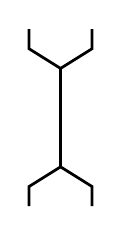
\begin{tikzpicture}[line width=1pt, yscale=.25, xscale=.8]
        \draw (1,9) -- (1,8) -- (.5,7) -- (.5,2) -- (1,1) -- (1,0);
        \draw (0,9) -- (0,8) -- (.5,7) -- (.5,2) -- (0,1) -- (0,0);
    \end{tikzpicture}
    \hspace{3cm}
    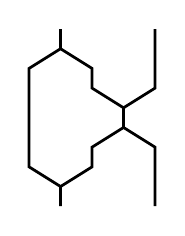
\begin{tikzpicture}[line width=1pt, yscale=.25, xscale=.8]
        \draw (0.5,9) -- (0.5,8) -- (0,7)                                         -- (0,2) -- (0.5,1) -- (0.5,0);
        \draw (0.5,9) -- (0.5,8) -- (1,7) -- (1,6) -- (1.5,5) -- (1.5,4) -- (1,3) -- (1,2) -- (0.5,1);
        \draw (2,9)   -- (2,6)                     -- (1.5,5) -- (1.5,4) -- (2,3)                     -- (2,0);
    \end{tikzpicture}
\]



% Weitere Symbole für das Symbolverzeichnis
\symbolindex[f]{$F$}{A topological or Riemann surface.}{}
\symbolindex[g]{$g$}{The genus of a surface or a slit domain.}{}
\symbolindex[m]{$m$}{The number of punctures respectively outgoing boundary curves of a surface or slit domain.}{}
\symbolindex[n]{$n$}{The number of (incomming) boundary curves of a surface of slit domain.}{}
\symbolindex[m]{$\Modspc \simeq B\Gamma_{g,n}^m$}{The moduli space of Riemann surfaces of genus $g$ with $m$ punctures and $n$ boundary curves.}{}
\symbolindex[g]{$\Gamma_{g,n}^m$}{The mapping class group with respect to $\Modspc$.}{}
\symbolindex[c]{$\C$}{The complex plane.}{}
\symbolindex[m]{$\mu$}{Either the product in the symmetric group or the product of two slit domains.}{Definition \ref{homology_operations:parallel_patching_slit_pics:mu}}
\symbolindex[s]{$\mathbb S^k$}{The $k$-dimensional sphere.}{}

% Symbolverzeichnis
\cleardoublepage        % Auch diese sollen auf der rechten Seite beginnen
\printnomenclature      % Symbolverzeichnis ausgeben

% Stichwortverzeichnis
\cleardoublepage        % Auch diese sollen auf der rechten Seite beginnen
\printindex             % Stichwortverzeichnis ausgeben

% Referenzen
\nocite{*}              % Alle Einträge der Bib-Datei sollen in die Referenzen
\cleardoublepage        % Auch diese sollen auf der rechten Seite beginnen
\printbibliography      % Bibliographie ausgeben.

\end{document}
